\documentclass[twoside]{book}

% Packages required by doxygen
\usepackage{fixltx2e}
\usepackage{calc}
\usepackage{doxygen}
\usepackage{graphicx}
\usepackage[utf8]{inputenc}
\usepackage{makeidx}
\usepackage{multicol}
\usepackage{multirow}
\PassOptionsToPackage{warn}{textcomp}
\usepackage{textcomp}
\usepackage[nointegrals]{wasysym}
\usepackage[table]{xcolor}

% Font selection
\usepackage[T1]{fontenc}
\usepackage{mathptmx}
\usepackage[scaled=.90]{helvet}
\usepackage{courier}
\usepackage{amssymb}
\usepackage{sectsty}
\renewcommand{\familydefault}{\sfdefault}
\allsectionsfont{%
  \fontseries{bc}\selectfont%
  \color{darkgray}%
}
\renewcommand{\DoxyLabelFont}{%
  \fontseries{bc}\selectfont%
  \color{darkgray}%
}
\newcommand{\+}{\discretionary{\mbox{\scriptsize$\hookleftarrow$}}{}{}}

% Page & text layout
\usepackage{geometry}
\geometry{%
  a4paper,%
  top=2.5cm,%
  bottom=2.5cm,%
  left=2.5cm,%
  right=2.5cm%
}
\tolerance=750
\hfuzz=15pt
\hbadness=750
\setlength{\emergencystretch}{15pt}
\setlength{\parindent}{0cm}
\setlength{\parskip}{0.2cm}
\makeatletter
\renewcommand{\paragraph}{%
  \@startsection{paragraph}{4}{0ex}{-1.0ex}{1.0ex}{%
    \normalfont\normalsize\bfseries\SS@parafont%
  }%
}
\renewcommand{\subparagraph}{%
  \@startsection{subparagraph}{5}{0ex}{-1.0ex}{1.0ex}{%
    \normalfont\normalsize\bfseries\SS@subparafont%
  }%
}
\makeatother

% Headers & footers
\usepackage{fancyhdr}
\pagestyle{fancyplain}
\fancyhead[LE]{\fancyplain{}{\bfseries\thepage}}
\fancyhead[CE]{\fancyplain{}{}}
\fancyhead[RE]{\fancyplain{}{\bfseries\leftmark}}
\fancyhead[LO]{\fancyplain{}{\bfseries\rightmark}}
\fancyhead[CO]{\fancyplain{}{}}
\fancyhead[RO]{\fancyplain{}{\bfseries\thepage}}
\fancyfoot[LE]{\fancyplain{}{}}
\fancyfoot[CE]{\fancyplain{}{}}
\fancyfoot[RE]{\fancyplain{}{\bfseries\scriptsize Generated on Thu Jan 14 2016 22\+:36\+:22 for Kalkulator\+Wymiany\+Walut by Doxygen }}
\fancyfoot[LO]{\fancyplain{}{\bfseries\scriptsize Generated on Thu Jan 14 2016 22\+:36\+:22 for Kalkulator\+Wymiany\+Walut by Doxygen }}
\fancyfoot[CO]{\fancyplain{}{}}
\fancyfoot[RO]{\fancyplain{}{}}
\renewcommand{\footrulewidth}{0.4pt}
\renewcommand{\chaptermark}[1]{%
  \markboth{#1}{}%
}
\renewcommand{\sectionmark}[1]{%
  \markright{\thesection\ #1}%
}

% Indices & bibliography
\usepackage{natbib}
\usepackage[titles]{tocloft}
\setcounter{tocdepth}{3}
\setcounter{secnumdepth}{5}
\makeindex

% Hyperlinks (required, but should be loaded last)
\usepackage{ifpdf}
\ifpdf
  \usepackage[pdftex,pagebackref=true]{hyperref}
\else
  \usepackage[ps2pdf,pagebackref=true]{hyperref}
\fi
\hypersetup{%
  colorlinks=true,%
  linkcolor=blue,%
  citecolor=blue,%
  unicode%
}

% Custom commands
\newcommand{\clearemptydoublepage}{%
  \newpage{\pagestyle{empty}\cleardoublepage}%
}


%===== C O N T E N T S =====

\begin{document}

% Titlepage & ToC
\hypersetup{pageanchor=false,
             bookmarks=true,
             bookmarksnumbered=true,
             pdfencoding=unicode
            }
\pagenumbering{roman}
\begin{titlepage}
\vspace*{7cm}
\begin{center}%
{\Large Kalkulator\+Wymiany\+Walut }\\
\vspace*{1cm}
{\large Generated by Doxygen 1.8.8}\\
\vspace*{0.5cm}
{\small Thu Jan 14 2016 22:36:22}\\
\end{center}
\end{titlepage}
\clearemptydoublepage
\tableofcontents
\clearemptydoublepage
\pagenumbering{arabic}
\hypersetup{pageanchor=true}

%--- Begin generated contents ---
\chapter{Namespace Index}
\section{Packages}
Here are the packages with brief descriptions (if available)\+:\begin{DoxyCompactList}
\item\contentsline{section}{\hyperlink{namespacekantor}{kantor} }{\pageref{namespacekantor}}{}
\item\contentsline{section}{\hyperlink{namespacekantor_1_1com}{kantor.\+com} }{\pageref{namespacekantor_1_1com}}{}
\item\contentsline{section}{\hyperlink{namespacekantor_1_1com_1_1web}{kantor.\+com.\+web} }{\pageref{namespacekantor_1_1com_1_1web}}{}
\item\contentsline{section}{\hyperlink{namespacekantor_1_1com_1_1web_1_1service}{kantor.\+com.\+web.\+service} }{\pageref{namespacekantor_1_1com_1_1web_1_1service}}{}
\end{DoxyCompactList}

\chapter{Hierarchical Index}
\section{Class Hierarchy}
This inheritance list is sorted roughly, but not completely, alphabetically\+:\begin{DoxyCompactList}
\item \contentsline{section}{kantor.\+com.\+web.\+service.\+Http\+Download\+Utility}{\pageref{classkantor_1_1com_1_1web_1_1service_1_1_http_download_utility}}{}
\item Remote\begin{DoxyCompactList}
\item \contentsline{section}{kantor.\+com.\+web.\+service.\+Kantor\+Przelicz}{\pageref{classkantor_1_1com_1_1web_1_1service_1_1_kantor_przelicz}}{}
\begin{DoxyCompactList}
\item \contentsline{section}{kantor.\+com.\+web.\+service.\+Kantor\+Przelicz\+Proxy}{\pageref{classkantor_1_1com_1_1web_1_1service_1_1_kantor_przelicz_proxy}}{}
\item \contentsline{section}{kantor.\+com.\+web.\+service.\+Kantor\+Przelicz\+Soap\+Binding\+Stub}{\pageref{classkantor_1_1com_1_1web_1_1service_1_1_kantor_przelicz_soap_binding_stub}}{}
\end{DoxyCompactList}
\item \contentsline{section}{kantor.\+com.\+web.\+service.\+Kursy\+Pokaz}{\pageref{classkantor_1_1com_1_1web_1_1service_1_1_kursy_pokaz}}{}
\begin{DoxyCompactList}
\item \contentsline{section}{kantor.\+com.\+web.\+service.\+Kursy\+Pokaz\+Proxy}{\pageref{classkantor_1_1com_1_1web_1_1service_1_1_kursy_pokaz_proxy}}{}
\item \contentsline{section}{kantor.\+com.\+web.\+service.\+Kursy\+Pokaz\+Soap\+Binding\+Stub}{\pageref{classkantor_1_1com_1_1web_1_1service_1_1_kursy_pokaz_soap_binding_stub}}{}
\end{DoxyCompactList}
\end{DoxyCompactList}
\item Service\begin{DoxyCompactList}
\item \contentsline{section}{kantor.\+com.\+web.\+service.\+Kantor\+Przelicz\+Service}{\pageref{interfacekantor_1_1com_1_1web_1_1service_1_1_kantor_przelicz_service}}{}
\begin{DoxyCompactList}
\item \contentsline{section}{kantor.\+com.\+web.\+service.\+Kantor\+Przelicz\+Service\+Locator}{\pageref{classkantor_1_1com_1_1web_1_1service_1_1_kantor_przelicz_service_locator}}{}
\end{DoxyCompactList}
\item \contentsline{section}{kantor.\+com.\+web.\+service.\+Kursy\+Pokaz\+Service}{\pageref{interfacekantor_1_1com_1_1web_1_1service_1_1_kursy_pokaz_service}}{}
\begin{DoxyCompactList}
\item \contentsline{section}{kantor.\+com.\+web.\+service.\+Kursy\+Pokaz\+Service\+Locator}{\pageref{classkantor_1_1com_1_1web_1_1service_1_1_kursy_pokaz_service_locator}}{}
\end{DoxyCompactList}
\end{DoxyCompactList}
\item Service\begin{DoxyCompactList}
\item \contentsline{section}{kantor.\+com.\+web.\+service.\+Kantor\+Przelicz\+Service\+Locator}{\pageref{classkantor_1_1com_1_1web_1_1service_1_1_kantor_przelicz_service_locator}}{}
\item \contentsline{section}{kantor.\+com.\+web.\+service.\+Kursy\+Pokaz\+Service\+Locator}{\pageref{classkantor_1_1com_1_1web_1_1service_1_1_kursy_pokaz_service_locator}}{}
\end{DoxyCompactList}
\item Stub\begin{DoxyCompactList}
\item \contentsline{section}{kantor.\+com.\+web.\+service.\+Kantor\+Przelicz\+Soap\+Binding\+Stub}{\pageref{classkantor_1_1com_1_1web_1_1service_1_1_kantor_przelicz_soap_binding_stub}}{}
\item \contentsline{section}{kantor.\+com.\+web.\+service.\+Kursy\+Pokaz\+Soap\+Binding\+Stub}{\pageref{classkantor_1_1com_1_1web_1_1service_1_1_kursy_pokaz_soap_binding_stub}}{}
\end{DoxyCompactList}
\end{DoxyCompactList}

\chapter{Class Index}
\section{Class List}
Here are the classes, structs, unions and interfaces with brief descriptions\+:\begin{DoxyCompactList}
\item\contentsline{section}{\hyperlink{classkantor_1_1com_1_1web_1_1service_1_1_http_download_utility}{kantor.\+com.\+web.\+service.\+Http\+Download\+Utility} }{\pageref{classkantor_1_1com_1_1web_1_1service_1_1_http_download_utility}}{}
\item\contentsline{section}{\hyperlink{classkantor_1_1com_1_1web_1_1service_1_1_kantor_przelicz}{kantor.\+com.\+web.\+service.\+Kantor\+Przelicz} }{\pageref{classkantor_1_1com_1_1web_1_1service_1_1_kantor_przelicz}}{}
\item\contentsline{section}{\hyperlink{classkantor_1_1com_1_1web_1_1service_1_1_kantor_przelicz_proxy}{kantor.\+com.\+web.\+service.\+Kantor\+Przelicz\+Proxy} }{\pageref{classkantor_1_1com_1_1web_1_1service_1_1_kantor_przelicz_proxy}}{}
\item\contentsline{section}{\hyperlink{interfacekantor_1_1com_1_1web_1_1service_1_1_kantor_przelicz_service}{kantor.\+com.\+web.\+service.\+Kantor\+Przelicz\+Service} }{\pageref{interfacekantor_1_1com_1_1web_1_1service_1_1_kantor_przelicz_service}}{}
\item\contentsline{section}{\hyperlink{classkantor_1_1com_1_1web_1_1service_1_1_kantor_przelicz_service_locator}{kantor.\+com.\+web.\+service.\+Kantor\+Przelicz\+Service\+Locator} }{\pageref{classkantor_1_1com_1_1web_1_1service_1_1_kantor_przelicz_service_locator}}{}
\item\contentsline{section}{\hyperlink{classkantor_1_1com_1_1web_1_1service_1_1_kantor_przelicz_soap_binding_stub}{kantor.\+com.\+web.\+service.\+Kantor\+Przelicz\+Soap\+Binding\+Stub} }{\pageref{classkantor_1_1com_1_1web_1_1service_1_1_kantor_przelicz_soap_binding_stub}}{}
\item\contentsline{section}{\hyperlink{classkantor_1_1com_1_1web_1_1service_1_1_kursy_pokaz}{kantor.\+com.\+web.\+service.\+Kursy\+Pokaz} }{\pageref{classkantor_1_1com_1_1web_1_1service_1_1_kursy_pokaz}}{}
\item\contentsline{section}{\hyperlink{classkantor_1_1com_1_1web_1_1service_1_1_kursy_pokaz_proxy}{kantor.\+com.\+web.\+service.\+Kursy\+Pokaz\+Proxy} }{\pageref{classkantor_1_1com_1_1web_1_1service_1_1_kursy_pokaz_proxy}}{}
\item\contentsline{section}{\hyperlink{interfacekantor_1_1com_1_1web_1_1service_1_1_kursy_pokaz_service}{kantor.\+com.\+web.\+service.\+Kursy\+Pokaz\+Service} }{\pageref{interfacekantor_1_1com_1_1web_1_1service_1_1_kursy_pokaz_service}}{}
\item\contentsline{section}{\hyperlink{classkantor_1_1com_1_1web_1_1service_1_1_kursy_pokaz_service_locator}{kantor.\+com.\+web.\+service.\+Kursy\+Pokaz\+Service\+Locator} }{\pageref{classkantor_1_1com_1_1web_1_1service_1_1_kursy_pokaz_service_locator}}{}
\item\contentsline{section}{\hyperlink{classkantor_1_1com_1_1web_1_1service_1_1_kursy_pokaz_soap_binding_stub}{kantor.\+com.\+web.\+service.\+Kursy\+Pokaz\+Soap\+Binding\+Stub} }{\pageref{classkantor_1_1com_1_1web_1_1service_1_1_kursy_pokaz_soap_binding_stub}}{}
\end{DoxyCompactList}

\chapter{File Index}
\section{File List}
Here is a list of all files with brief descriptions\+:\begin{DoxyCompactList}
\item\contentsline{section}{C\+:/\+Users/kuska/\+Desktop/\+Michalik/\+K\+W/html/\hyperlink{dynsections_8js}{dynsections.\+js} }{\pageref{dynsections_8js}}{}
\item\contentsline{section}{C\+:/\+Users/kuska/\+Desktop/\+Michalik/\+K\+W/html/\hyperlink{jquery_8js}{jquery.\+js} }{\pageref{jquery_8js}}{}
\item\contentsline{section}{C\+:/\+Users/kuska/\+Desktop/\+Michalik/\+K\+W/html/search/\hyperlink{all__0_8js}{all\+\_\+0.\+js} }{\pageref{all__0_8js}}{}
\item\contentsline{section}{C\+:/\+Users/kuska/\+Desktop/\+Michalik/\+K\+W/html/search/\hyperlink{all__1_8js}{all\+\_\+1.\+js} }{\pageref{all__1_8js}}{}
\item\contentsline{section}{C\+:/\+Users/kuska/\+Desktop/\+Michalik/\+K\+W/html/search/\hyperlink{all__2_8js}{all\+\_\+2.\+js} }{\pageref{all__2_8js}}{}
\item\contentsline{section}{C\+:/\+Users/kuska/\+Desktop/\+Michalik/\+K\+W/html/search/\hyperlink{all__3_8js}{all\+\_\+3.\+js} }{\pageref{all__3_8js}}{}
\item\contentsline{section}{C\+:/\+Users/kuska/\+Desktop/\+Michalik/\+K\+W/html/search/\hyperlink{all__4_8js}{all\+\_\+4.\+js} }{\pageref{all__4_8js}}{}
\item\contentsline{section}{C\+:/\+Users/kuska/\+Desktop/\+Michalik/\+K\+W/html/search/\hyperlink{all__5_8js}{all\+\_\+5.\+js} }{\pageref{all__5_8js}}{}
\item\contentsline{section}{C\+:/\+Users/kuska/\+Desktop/\+Michalik/\+K\+W/html/search/\hyperlink{all__6_8js}{all\+\_\+6.\+js} }{\pageref{all__6_8js}}{}
\item\contentsline{section}{C\+:/\+Users/kuska/\+Desktop/\+Michalik/\+K\+W/html/search/\hyperlink{all__7_8js}{all\+\_\+7.\+js} }{\pageref{all__7_8js}}{}
\item\contentsline{section}{C\+:/\+Users/kuska/\+Desktop/\+Michalik/\+K\+W/html/search/\hyperlink{all__8_8js}{all\+\_\+8.\+js} }{\pageref{all__8_8js}}{}
\item\contentsline{section}{C\+:/\+Users/kuska/\+Desktop/\+Michalik/\+K\+W/html/search/\hyperlink{all__9_8js}{all\+\_\+9.\+js} }{\pageref{all__9_8js}}{}
\item\contentsline{section}{C\+:/\+Users/kuska/\+Desktop/\+Michalik/\+K\+W/html/search/\hyperlink{all__a_8js}{all\+\_\+a.\+js} }{\pageref{all__a_8js}}{}
\item\contentsline{section}{C\+:/\+Users/kuska/\+Desktop/\+Michalik/\+K\+W/html/search/\hyperlink{classes__0_8js}{classes\+\_\+0.\+js} }{\pageref{classes__0_8js}}{}
\item\contentsline{section}{C\+:/\+Users/kuska/\+Desktop/\+Michalik/\+K\+W/html/search/\hyperlink{classes__1_8js}{classes\+\_\+1.\+js} }{\pageref{classes__1_8js}}{}
\item\contentsline{section}{C\+:/\+Users/kuska/\+Desktop/\+Michalik/\+K\+W/html/search/\hyperlink{files__0_8js}{files\+\_\+0.\+js} }{\pageref{files__0_8js}}{}
\item\contentsline{section}{C\+:/\+Users/kuska/\+Desktop/\+Michalik/\+K\+W/html/search/\hyperlink{files__1_8js}{files\+\_\+1.\+js} }{\pageref{files__1_8js}}{}
\item\contentsline{section}{C\+:/\+Users/kuska/\+Desktop/\+Michalik/\+K\+W/html/search/\hyperlink{functions__0_8js}{functions\+\_\+0.\+js} }{\pageref{functions__0_8js}}{}
\item\contentsline{section}{C\+:/\+Users/kuska/\+Desktop/\+Michalik/\+K\+W/html/search/\hyperlink{functions__1_8js}{functions\+\_\+1.\+js} }{\pageref{functions__1_8js}}{}
\item\contentsline{section}{C\+:/\+Users/kuska/\+Desktop/\+Michalik/\+K\+W/html/search/\hyperlink{functions__2_8js}{functions\+\_\+2.\+js} }{\pageref{functions__2_8js}}{}
\item\contentsline{section}{C\+:/\+Users/kuska/\+Desktop/\+Michalik/\+K\+W/html/search/\hyperlink{functions__3_8js}{functions\+\_\+3.\+js} }{\pageref{functions__3_8js}}{}
\item\contentsline{section}{C\+:/\+Users/kuska/\+Desktop/\+Michalik/\+K\+W/html/search/\hyperlink{functions__4_8js}{functions\+\_\+4.\+js} }{\pageref{functions__4_8js}}{}
\item\contentsline{section}{C\+:/\+Users/kuska/\+Desktop/\+Michalik/\+K\+W/html/search/\hyperlink{functions__5_8js}{functions\+\_\+5.\+js} }{\pageref{functions__5_8js}}{}
\item\contentsline{section}{C\+:/\+Users/kuska/\+Desktop/\+Michalik/\+K\+W/html/search/\hyperlink{functions__6_8js}{functions\+\_\+6.\+js} }{\pageref{functions__6_8js}}{}
\item\contentsline{section}{C\+:/\+Users/kuska/\+Desktop/\+Michalik/\+K\+W/html/search/\hyperlink{functions__7_8js}{functions\+\_\+7.\+js} }{\pageref{functions__7_8js}}{}
\item\contentsline{section}{C\+:/\+Users/kuska/\+Desktop/\+Michalik/\+K\+W/html/search/\hyperlink{functions__8_8js}{functions\+\_\+8.\+js} }{\pageref{functions__8_8js}}{}
\item\contentsline{section}{C\+:/\+Users/kuska/\+Desktop/\+Michalik/\+K\+W/html/search/\hyperlink{functions__9_8js}{functions\+\_\+9.\+js} }{\pageref{functions__9_8js}}{}
\item\contentsline{section}{C\+:/\+Users/kuska/\+Desktop/\+Michalik/\+K\+W/html/search/\hyperlink{namespaces__0_8js}{namespaces\+\_\+0.\+js} }{\pageref{namespaces__0_8js}}{}
\item\contentsline{section}{C\+:/\+Users/kuska/\+Desktop/\+Michalik/\+K\+W/html/search/\hyperlink{search_8js}{search.\+js} }{\pageref{search_8js}}{}
\item\contentsline{section}{C\+:/\+Users/kuska/\+Desktop/\+Michalik/\+K\+W/\+Kantor\+W\+S/src/kantor/com/web/service/\hyperlink{_http_download_utility_8java}{Http\+Download\+Utility.\+java} }{\pageref{_http_download_utility_8java}}{}
\item\contentsline{section}{C\+:/\+Users/kuska/\+Desktop/\+Michalik/\+K\+W/\+Kantor\+W\+S/src/kantor/com/web/service/\hyperlink{src_2kantor_2com_2web_2service_2_kantor_przelicz_8java}{Kantor\+Przelicz.\+java} }{\pageref{src_2kantor_2com_2web_2service_2_kantor_przelicz_8java}}{}
\item\contentsline{section}{C\+:/\+Users/kuska/\+Desktop/\+Michalik/\+K\+W/\+Kantor\+W\+S/src/kantor/com/web/service/\hyperlink{src_2kantor_2com_2web_2service_2_kursy_pokaz_8java}{Kursy\+Pokaz.\+java} }{\pageref{src_2kantor_2com_2web_2service_2_kursy_pokaz_8java}}{}
\item\contentsline{section}{C\+:/\+Users/kuska/\+Desktop/\+Michalik/\+K\+W/\+Kantor\+W\+S\+Client/src/kantor/com/web/service/\hyperlink{lient_2src_2kantor_2com_2web_2service_2_kantor_przelicz_8java}{Kantor\+Przelicz.\+java} }{\pageref{lient_2src_2kantor_2com_2web_2service_2_kantor_przelicz_8java}}{}
\item\contentsline{section}{C\+:/\+Users/kuska/\+Desktop/\+Michalik/\+K\+W/\+Kantor\+W\+S\+Client/src/kantor/com/web/service/\hyperlink{_kantor_przelicz_proxy_8java}{Kantor\+Przelicz\+Proxy.\+java} }{\pageref{_kantor_przelicz_proxy_8java}}{}
\item\contentsline{section}{C\+:/\+Users/kuska/\+Desktop/\+Michalik/\+K\+W/\+Kantor\+W\+S\+Client/src/kantor/com/web/service/\hyperlink{_kantor_przelicz_service_8java}{Kantor\+Przelicz\+Service.\+java} }{\pageref{_kantor_przelicz_service_8java}}{}
\item\contentsline{section}{C\+:/\+Users/kuska/\+Desktop/\+Michalik/\+K\+W/\+Kantor\+W\+S\+Client/src/kantor/com/web/service/\hyperlink{_kantor_przelicz_service_locator_8java}{Kantor\+Przelicz\+Service\+Locator.\+java} }{\pageref{_kantor_przelicz_service_locator_8java}}{}
\item\contentsline{section}{C\+:/\+Users/kuska/\+Desktop/\+Michalik/\+K\+W/\+Kantor\+W\+S\+Client/src/kantor/com/web/service/\hyperlink{_kantor_przelicz_soap_binding_stub_8java}{Kantor\+Przelicz\+Soap\+Binding\+Stub.\+java} }{\pageref{_kantor_przelicz_soap_binding_stub_8java}}{}
\item\contentsline{section}{C\+:/\+Users/kuska/\+Desktop/\+Michalik/\+K\+W/\+Kantor\+W\+S\+Client/src/kantor/com/web/service/\hyperlink{lient_2src_2kantor_2com_2web_2service_2_kursy_pokaz_8java}{Kursy\+Pokaz.\+java} }{\pageref{lient_2src_2kantor_2com_2web_2service_2_kursy_pokaz_8java}}{}
\item\contentsline{section}{C\+:/\+Users/kuska/\+Desktop/\+Michalik/\+K\+W/\+Kantor\+W\+S\+Client/src/kantor/com/web/service/\hyperlink{_kursy_pokaz_proxy_8java}{Kursy\+Pokaz\+Proxy.\+java} }{\pageref{_kursy_pokaz_proxy_8java}}{}
\item\contentsline{section}{C\+:/\+Users/kuska/\+Desktop/\+Michalik/\+K\+W/\+Kantor\+W\+S\+Client/src/kantor/com/web/service/\hyperlink{_kursy_pokaz_service_8java}{Kursy\+Pokaz\+Service.\+java} }{\pageref{_kursy_pokaz_service_8java}}{}
\item\contentsline{section}{C\+:/\+Users/kuska/\+Desktop/\+Michalik/\+K\+W/\+Kantor\+W\+S\+Client/src/kantor/com/web/service/\hyperlink{_kursy_pokaz_service_locator_8java}{Kursy\+Pokaz\+Service\+Locator.\+java} }{\pageref{_kursy_pokaz_service_locator_8java}}{}
\item\contentsline{section}{C\+:/\+Users/kuska/\+Desktop/\+Michalik/\+K\+W/\+Kantor\+W\+S\+Client/src/kantor/com/web/service/\hyperlink{_kursy_pokaz_soap_binding_stub_8java}{Kursy\+Pokaz\+Soap\+Binding\+Stub.\+java} }{\pageref{_kursy_pokaz_soap_binding_stub_8java}}{}
\end{DoxyCompactList}

\chapter{Namespace Documentation}
\hypertarget{namespacekantor}{\section{Package kantor}
\label{namespacekantor}\index{kantor@{kantor}}
}
\subsection*{Packages}
\begin{DoxyCompactItemize}
\item 
package \hyperlink{namespacekantor_1_1com}{com}
\end{DoxyCompactItemize}

\hypertarget{namespacekantor_1_1com}{\section{Package kantor.\+com}
\label{namespacekantor_1_1com}\index{kantor.\+com@{kantor.\+com}}
}
\subsection*{Packages}
\begin{DoxyCompactItemize}
\item 
package \hyperlink{namespacekantor_1_1com_1_1web}{web}
\end{DoxyCompactItemize}

\hypertarget{namespacekantor_1_1com_1_1web}{\section{Package kantor.\+com.\+web}
\label{namespacekantor_1_1com_1_1web}\index{kantor.\+com.\+web@{kantor.\+com.\+web}}
}
\subsection*{Packages}
\begin{DoxyCompactItemize}
\item 
package \hyperlink{namespacekantor_1_1com_1_1web_1_1service}{service}
\end{DoxyCompactItemize}

\hypertarget{namespacekantor_1_1com_1_1web_1_1service}{\section{Package kantor.\+com.\+web.\+service}
\label{namespacekantor_1_1com_1_1web_1_1service}\index{kantor.\+com.\+web.\+service@{kantor.\+com.\+web.\+service}}
}
\subsection*{Classes}
\begin{DoxyCompactItemize}
\item 
class \hyperlink{classkantor_1_1com_1_1web_1_1service_1_1_http_download_utility}{Http\+Download\+Utility}
\item 
interface \hyperlink{classkantor_1_1com_1_1web_1_1service_1_1_kantor_przelicz}{Kantor\+Przelicz}
\item 
class \hyperlink{classkantor_1_1com_1_1web_1_1service_1_1_kantor_przelicz_proxy}{Kantor\+Przelicz\+Proxy}
\item 
interface \hyperlink{interfacekantor_1_1com_1_1web_1_1service_1_1_kantor_przelicz_service}{Kantor\+Przelicz\+Service}
\item 
class \hyperlink{classkantor_1_1com_1_1web_1_1service_1_1_kantor_przelicz_service_locator}{Kantor\+Przelicz\+Service\+Locator}
\item 
class \hyperlink{classkantor_1_1com_1_1web_1_1service_1_1_kantor_przelicz_soap_binding_stub}{Kantor\+Przelicz\+Soap\+Binding\+Stub}
\item 
interface \hyperlink{classkantor_1_1com_1_1web_1_1service_1_1_kursy_pokaz}{Kursy\+Pokaz}
\item 
class \hyperlink{classkantor_1_1com_1_1web_1_1service_1_1_kursy_pokaz_proxy}{Kursy\+Pokaz\+Proxy}
\item 
interface \hyperlink{interfacekantor_1_1com_1_1web_1_1service_1_1_kursy_pokaz_service}{Kursy\+Pokaz\+Service}
\item 
class \hyperlink{classkantor_1_1com_1_1web_1_1service_1_1_kursy_pokaz_service_locator}{Kursy\+Pokaz\+Service\+Locator}
\item 
class \hyperlink{classkantor_1_1com_1_1web_1_1service_1_1_kursy_pokaz_soap_binding_stub}{Kursy\+Pokaz\+Soap\+Binding\+Stub}
\end{DoxyCompactItemize}


\subsection{Detailed Description}
Kantor\+Przelicz.\+java

This file was auto-\/generated from W\+S\+D\+L by the Apache Axis 1.\+4 Apr 22, 2006 (06\+:55\+:48 P\+D\+T) W\+S\+D\+L2\+Java emitter.

\hyperlink{_kantor_przelicz_service_8java}{Kantor\+Przelicz\+Service.\+java}

This file was auto-\/generated from W\+S\+D\+L by the Apache Axis 1.\+4 Apr 22, 2006 (06\+:55\+:48 P\+D\+T) W\+S\+D\+L2\+Java emitter.

\hyperlink{_kantor_przelicz_service_locator_8java}{Kantor\+Przelicz\+Service\+Locator.\+java}

This file was auto-\/generated from W\+S\+D\+L by the Apache Axis 1.\+4 Apr 22, 2006 (06\+:55\+:48 P\+D\+T) W\+S\+D\+L2\+Java emitter.

\hyperlink{_kantor_przelicz_soap_binding_stub_8java}{Kantor\+Przelicz\+Soap\+Binding\+Stub.\+java}

This file was auto-\/generated from W\+S\+D\+L by the Apache Axis 1.\+4 Apr 22, 2006 (06\+:55\+:48 P\+D\+T) W\+S\+D\+L2\+Java emitter.

Kursy\+Pokaz.\+java

This file was auto-\/generated from W\+S\+D\+L by the Apache Axis 1.\+4 Apr 22, 2006 (06\+:55\+:48 P\+D\+T) W\+S\+D\+L2\+Java emitter.

\hyperlink{_kursy_pokaz_service_8java}{Kursy\+Pokaz\+Service.\+java}

This file was auto-\/generated from W\+S\+D\+L by the Apache Axis 1.\+4 Apr 22, 2006 (06\+:55\+:48 P\+D\+T) W\+S\+D\+L2\+Java emitter.

\hyperlink{_kursy_pokaz_service_locator_8java}{Kursy\+Pokaz\+Service\+Locator.\+java}

This file was auto-\/generated from W\+S\+D\+L by the Apache Axis 1.\+4 Apr 22, 2006 (06\+:55\+:48 P\+D\+T) W\+S\+D\+L2\+Java emitter.

\hyperlink{_kursy_pokaz_soap_binding_stub_8java}{Kursy\+Pokaz\+Soap\+Binding\+Stub.\+java}

This file was auto-\/generated from W\+S\+D\+L by the Apache Axis 1.\+4 Apr 22, 2006 (06\+:55\+:48 P\+D\+T) W\+S\+D\+L2\+Java emitter. 
\chapter{Class Documentation}
\hypertarget{classkantor_1_1com_1_1web_1_1service_1_1_http_download_utility}{\section{kantor.\+com.\+web.\+service.\+Http\+Download\+Utility Class Reference}
\label{classkantor_1_1com_1_1web_1_1service_1_1_http_download_utility}\index{kantor.\+com.\+web.\+service.\+Http\+Download\+Utility@{kantor.\+com.\+web.\+service.\+Http\+Download\+Utility}}
}
\subsection*{Static Public Member Functions}
\begin{DoxyCompactItemize}
\item 
static void \hyperlink{classkantor_1_1com_1_1web_1_1service_1_1_http_download_utility_abf7fe23e59e57f8d7b467c5cc63e6aae}{download\+File} (String file\+U\+R\+L, String save\+Dir)  throws I\+O\+Exception 
\end{DoxyCompactItemize}


\subsection{Detailed Description}


Definition at line 11 of file Http\+Download\+Utility.\+java.



\subsection{Member Function Documentation}
\hypertarget{classkantor_1_1com_1_1web_1_1service_1_1_http_download_utility_abf7fe23e59e57f8d7b467c5cc63e6aae}{\index{kantor\+::com\+::web\+::service\+::\+Http\+Download\+Utility@{kantor\+::com\+::web\+::service\+::\+Http\+Download\+Utility}!download\+File@{download\+File}}
\index{download\+File@{download\+File}!kantor\+::com\+::web\+::service\+::\+Http\+Download\+Utility@{kantor\+::com\+::web\+::service\+::\+Http\+Download\+Utility}}
\subsubsection[{download\+File}]{\setlength{\rightskip}{0pt plus 5cm}static void kantor.\+com.\+web.\+service.\+Http\+Download\+Utility.\+download\+File (
\begin{DoxyParamCaption}
\item[{String}]{file\+U\+R\+L, }
\item[{String}]{save\+Dir}
\end{DoxyParamCaption}
) throws I\+O\+Exception\hspace{0.3cm}{\ttfamily [static]}}}\label{classkantor_1_1com_1_1web_1_1service_1_1_http_download_utility_abf7fe23e59e57f8d7b467c5cc63e6aae}
Downloads a file from a U\+R\+L 
\begin{DoxyParams}{Parameters}
{\em file\+U\+R\+L} & H\+T\+T\+P U\+R\+L of the file to be downloaded \\
\hline
{\em save\+Dir} & path of the directory to save the file \\
\hline
\end{DoxyParams}

\begin{DoxyExceptions}{Exceptions}
{\em I\+O\+Exception} & \\
\hline
\end{DoxyExceptions}


Definition at line 21 of file Http\+Download\+Utility.\+java.



The documentation for this class was generated from the following file\+:\begin{DoxyCompactItemize}
\item 
C\+:/\+Users/kuska/\+Desktop/\+Michalik/\+K\+W/\+Kantor\+W\+S/src/kantor/com/web/service/\hyperlink{_http_download_utility_8java}{Http\+Download\+Utility.\+java}\end{DoxyCompactItemize}

\hypertarget{classkantor_1_1com_1_1web_1_1service_1_1_kantor_przelicz}{\section{kantor.\+com.\+web.\+service.\+Kantor\+Przelicz Interface Reference}
\label{classkantor_1_1com_1_1web_1_1service_1_1_kantor_przelicz}\index{kantor.\+com.\+web.\+service.\+Kantor\+Przelicz@{kantor.\+com.\+web.\+service.\+Kantor\+Przelicz}}
}
Inheritance diagram for kantor.\+com.\+web.\+service.\+Kantor\+Przelicz\+:\begin{figure}[H]
\begin{center}
\leavevmode

\includegraphics[height=2.492581cm]{classkantor_1_1com_1_1web_1_1service_1_1_kantor_przelicz}
\end{center}
\end{figure}
\subsection*{Public Member Functions}
\begin{DoxyCompactItemize}
\item 
double \hyperlink{classkantor_1_1com_1_1web_1_1service_1_1_kantor_przelicz_ad263683559db773d4ccb28e14090824f}{U\+S\+Dna\+P\+L\+N} (double value)
\item 
double \hyperlink{classkantor_1_1com_1_1web_1_1service_1_1_kantor_przelicz_aea3a5dd74cf10d0c9ce1bf04b94078c8}{P\+L\+Nna\+U\+S\+D} (double value)
\item 
double \hyperlink{classkantor_1_1com_1_1web_1_1service_1_1_kantor_przelicz_af204b150c62165c836a1a0afd10c16b7}{E\+U\+Rna\+P\+L\+N} (double value)
\item 
double \hyperlink{classkantor_1_1com_1_1web_1_1service_1_1_kantor_przelicz_acfc0cd42fb64c5f26d468245cf0fe3b6}{P\+L\+Nna\+E\+U\+R} (double value)
\item 
double \hyperlink{classkantor_1_1com_1_1web_1_1service_1_1_kantor_przelicz_acff8492d50d84cf718bca4c8b499d36a}{C\+H\+Ena\+P\+L\+N} (double value)
\item 
double \hyperlink{classkantor_1_1com_1_1web_1_1service_1_1_kantor_przelicz_afa953802446690d409e1df5361729fc0}{P\+L\+Nna\+C\+H\+E} (double value)
\item 
double \hyperlink{classkantor_1_1com_1_1web_1_1service_1_1_kantor_przelicz_a64b58db5e686a08b4b1af648eb781a1c}{G\+B\+Pna\+P\+L\+N} (double value)
\item 
double \hyperlink{classkantor_1_1com_1_1web_1_1service_1_1_kantor_przelicz_ad0840077798f333f948772590d1a402a}{P\+L\+Nna\+G\+B\+P} (double value)
\item 
double \hyperlink{classkantor_1_1com_1_1web_1_1service_1_1_kantor_przelicz_a9e6f2e71874e1dd7b520d2da4427bae8}{J\+P\+Yna\+P\+L\+N} (double value)
\item 
double \hyperlink{classkantor_1_1com_1_1web_1_1service_1_1_kantor_przelicz_a7706e3a08c1b8ce3775506c4530d1bf7}{P\+L\+Nna\+J\+P\+Y} (double value)
\item 
double \hyperlink{classkantor_1_1com_1_1web_1_1service_1_1_kantor_przelicz_a11c3958baf84a3a96dbc9290890b6c4e}{R\+U\+Bna\+P\+L\+N} (double value)
\item 
double \hyperlink{classkantor_1_1com_1_1web_1_1service_1_1_kantor_przelicz_ad68cbeb18f18cd02c3b4b571da0e06fa}{P\+L\+Nna\+R\+U\+B} (double value)
\item 
double\mbox{[}$\,$\mbox{]} \hyperlink{classkantor_1_1com_1_1web_1_1service_1_1_kantor_przelicz_a9e2610a2cdb76ea7e2551786f3c0736e}{pobierz\+\_\+kursy\+\_\+walut} ()
\item 
double\mbox{[}$\,$\mbox{]} \hyperlink{classkantor_1_1com_1_1web_1_1service_1_1_kantor_przelicz_a9e2610a2cdb76ea7e2551786f3c0736e}{pobierz\+\_\+kursy\+\_\+walut} ()  throws java.\+rmi.\+Remote\+Exception
\item 
double \hyperlink{classkantor_1_1com_1_1web_1_1service_1_1_kantor_przelicz_a64b58db5e686a08b4b1af648eb781a1c}{G\+B\+Pna\+P\+L\+N} (double value)  throws java.\+rmi.\+Remote\+Exception
\item 
double \hyperlink{classkantor_1_1com_1_1web_1_1service_1_1_kantor_przelicz_ad68cbeb18f18cd02c3b4b571da0e06fa}{P\+L\+Nna\+R\+U\+B} (double value)  throws java.\+rmi.\+Remote\+Exception
\item 
double \hyperlink{classkantor_1_1com_1_1web_1_1service_1_1_kantor_przelicz_a9e6f2e71874e1dd7b520d2da4427bae8}{J\+P\+Yna\+P\+L\+N} (double value)  throws java.\+rmi.\+Remote\+Exception
\item 
double \hyperlink{classkantor_1_1com_1_1web_1_1service_1_1_kantor_przelicz_ad0840077798f333f948772590d1a402a}{P\+L\+Nna\+G\+B\+P} (double value)  throws java.\+rmi.\+Remote\+Exception
\item 
double \hyperlink{classkantor_1_1com_1_1web_1_1service_1_1_kantor_przelicz_a7706e3a08c1b8ce3775506c4530d1bf7}{P\+L\+Nna\+J\+P\+Y} (double value)  throws java.\+rmi.\+Remote\+Exception
\item 
double \hyperlink{classkantor_1_1com_1_1web_1_1service_1_1_kantor_przelicz_a11c3958baf84a3a96dbc9290890b6c4e}{R\+U\+Bna\+P\+L\+N} (double value)  throws java.\+rmi.\+Remote\+Exception
\item 
double \hyperlink{classkantor_1_1com_1_1web_1_1service_1_1_kantor_przelicz_ad263683559db773d4ccb28e14090824f}{U\+S\+Dna\+P\+L\+N} (double value)  throws java.\+rmi.\+Remote\+Exception
\item 
double \hyperlink{classkantor_1_1com_1_1web_1_1service_1_1_kantor_przelicz_aea3a5dd74cf10d0c9ce1bf04b94078c8}{P\+L\+Nna\+U\+S\+D} (double value)  throws java.\+rmi.\+Remote\+Exception
\item 
double \hyperlink{classkantor_1_1com_1_1web_1_1service_1_1_kantor_przelicz_af204b150c62165c836a1a0afd10c16b7}{E\+U\+Rna\+P\+L\+N} (double value)  throws java.\+rmi.\+Remote\+Exception
\item 
double \hyperlink{classkantor_1_1com_1_1web_1_1service_1_1_kantor_przelicz_acfc0cd42fb64c5f26d468245cf0fe3b6}{P\+L\+Nna\+E\+U\+R} (double value)  throws java.\+rmi.\+Remote\+Exception
\item 
double \hyperlink{classkantor_1_1com_1_1web_1_1service_1_1_kantor_przelicz_afa953802446690d409e1df5361729fc0}{P\+L\+Nna\+C\+H\+E} (double value)  throws java.\+rmi.\+Remote\+Exception
\item 
double \hyperlink{classkantor_1_1com_1_1web_1_1service_1_1_kantor_przelicz_acff8492d50d84cf718bca4c8b499d36a}{C\+H\+Ena\+P\+L\+N} (double value)  throws java.\+rmi.\+Remote\+Exception
\end{DoxyCompactItemize}


\subsection{Detailed Description}


Definition at line 15 of file Kantor\+Przelicz.\+java.



\subsection{Member Function Documentation}
\hypertarget{classkantor_1_1com_1_1web_1_1service_1_1_kantor_przelicz_acff8492d50d84cf718bca4c8b499d36a}{\index{kantor\+::com\+::web\+::service\+::\+Kantor\+Przelicz@{kantor\+::com\+::web\+::service\+::\+Kantor\+Przelicz}!C\+H\+Ena\+P\+L\+N@{C\+H\+Ena\+P\+L\+N}}
\index{C\+H\+Ena\+P\+L\+N@{C\+H\+Ena\+P\+L\+N}!kantor\+::com\+::web\+::service\+::\+Kantor\+Przelicz@{kantor\+::com\+::web\+::service\+::\+Kantor\+Przelicz}}
\subsubsection[{C\+H\+Ena\+P\+L\+N}]{\setlength{\rightskip}{0pt plus 5cm}double kantor.\+com.\+web.\+service.\+Kantor\+Przelicz.\+C\+H\+Ena\+P\+L\+N (
\begin{DoxyParamCaption}
\item[{double}]{value}
\end{DoxyParamCaption}
) throws java.\+rmi.\+Remote\+Exception}}\label{classkantor_1_1com_1_1web_1_1service_1_1_kantor_przelicz_acff8492d50d84cf718bca4c8b499d36a}


Implemented in \hyperlink{classkantor_1_1com_1_1web_1_1service_1_1_kantor_przelicz_soap_binding_stub_a95c3905cd703617b5c0355134546befc}{kantor.\+com.\+web.\+service.\+Kantor\+Przelicz\+Soap\+Binding\+Stub}, and \hyperlink{classkantor_1_1com_1_1web_1_1service_1_1_kantor_przelicz_proxy_a3e40e9d8fb68c3edc8d0301b2fe524b6}{kantor.\+com.\+web.\+service.\+Kantor\+Przelicz\+Proxy}.

\hypertarget{classkantor_1_1com_1_1web_1_1service_1_1_kantor_przelicz_acff8492d50d84cf718bca4c8b499d36a}{\index{kantor\+::com\+::web\+::service\+::\+Kantor\+Przelicz@{kantor\+::com\+::web\+::service\+::\+Kantor\+Przelicz}!C\+H\+Ena\+P\+L\+N@{C\+H\+Ena\+P\+L\+N}}
\index{C\+H\+Ena\+P\+L\+N@{C\+H\+Ena\+P\+L\+N}!kantor\+::com\+::web\+::service\+::\+Kantor\+Przelicz@{kantor\+::com\+::web\+::service\+::\+Kantor\+Przelicz}}
\subsubsection[{C\+H\+Ena\+P\+L\+N}]{\setlength{\rightskip}{0pt plus 5cm}double kantor.\+com.\+web.\+service.\+Kantor\+Przelicz.\+C\+H\+Ena\+P\+L\+N (
\begin{DoxyParamCaption}
\item[{double}]{value}
\end{DoxyParamCaption}
)}}\label{classkantor_1_1com_1_1web_1_1service_1_1_kantor_przelicz_acff8492d50d84cf718bca4c8b499d36a}


Implemented in \hyperlink{classkantor_1_1com_1_1web_1_1service_1_1_kantor_przelicz_soap_binding_stub_a95c3905cd703617b5c0355134546befc}{kantor.\+com.\+web.\+service.\+Kantor\+Przelicz\+Soap\+Binding\+Stub}, and \hyperlink{classkantor_1_1com_1_1web_1_1service_1_1_kantor_przelicz_proxy_a3e40e9d8fb68c3edc8d0301b2fe524b6}{kantor.\+com.\+web.\+service.\+Kantor\+Przelicz\+Proxy}.



Definition at line 73 of file Kantor\+Przelicz.\+java.

\hypertarget{classkantor_1_1com_1_1web_1_1service_1_1_kantor_przelicz_af204b150c62165c836a1a0afd10c16b7}{\index{kantor\+::com\+::web\+::service\+::\+Kantor\+Przelicz@{kantor\+::com\+::web\+::service\+::\+Kantor\+Przelicz}!E\+U\+Rna\+P\+L\+N@{E\+U\+Rna\+P\+L\+N}}
\index{E\+U\+Rna\+P\+L\+N@{E\+U\+Rna\+P\+L\+N}!kantor\+::com\+::web\+::service\+::\+Kantor\+Przelicz@{kantor\+::com\+::web\+::service\+::\+Kantor\+Przelicz}}
\subsubsection[{E\+U\+Rna\+P\+L\+N}]{\setlength{\rightskip}{0pt plus 5cm}double kantor.\+com.\+web.\+service.\+Kantor\+Przelicz.\+E\+U\+Rna\+P\+L\+N (
\begin{DoxyParamCaption}
\item[{double}]{value}
\end{DoxyParamCaption}
) throws java.\+rmi.\+Remote\+Exception}}\label{classkantor_1_1com_1_1web_1_1service_1_1_kantor_przelicz_af204b150c62165c836a1a0afd10c16b7}


Implemented in \hyperlink{classkantor_1_1com_1_1web_1_1service_1_1_kantor_przelicz_soap_binding_stub_a1ca4bcdbf6b3301c515be2ddb81a7689}{kantor.\+com.\+web.\+service.\+Kantor\+Przelicz\+Soap\+Binding\+Stub}, and \hyperlink{classkantor_1_1com_1_1web_1_1service_1_1_kantor_przelicz_proxy_afcaaed0493d9da86ff7eb4d6fb3a7e6d}{kantor.\+com.\+web.\+service.\+Kantor\+Przelicz\+Proxy}.

\hypertarget{classkantor_1_1com_1_1web_1_1service_1_1_kantor_przelicz_af204b150c62165c836a1a0afd10c16b7}{\index{kantor\+::com\+::web\+::service\+::\+Kantor\+Przelicz@{kantor\+::com\+::web\+::service\+::\+Kantor\+Przelicz}!E\+U\+Rna\+P\+L\+N@{E\+U\+Rna\+P\+L\+N}}
\index{E\+U\+Rna\+P\+L\+N@{E\+U\+Rna\+P\+L\+N}!kantor\+::com\+::web\+::service\+::\+Kantor\+Przelicz@{kantor\+::com\+::web\+::service\+::\+Kantor\+Przelicz}}
\subsubsection[{E\+U\+Rna\+P\+L\+N}]{\setlength{\rightskip}{0pt plus 5cm}double kantor.\+com.\+web.\+service.\+Kantor\+Przelicz.\+E\+U\+Rna\+P\+L\+N (
\begin{DoxyParamCaption}
\item[{double}]{value}
\end{DoxyParamCaption}
)}}\label{classkantor_1_1com_1_1web_1_1service_1_1_kantor_przelicz_af204b150c62165c836a1a0afd10c16b7}


Implemented in \hyperlink{classkantor_1_1com_1_1web_1_1service_1_1_kantor_przelicz_soap_binding_stub_a1ca4bcdbf6b3301c515be2ddb81a7689}{kantor.\+com.\+web.\+service.\+Kantor\+Przelicz\+Soap\+Binding\+Stub}, and \hyperlink{classkantor_1_1com_1_1web_1_1service_1_1_kantor_przelicz_proxy_afcaaed0493d9da86ff7eb4d6fb3a7e6d}{kantor.\+com.\+web.\+service.\+Kantor\+Przelicz\+Proxy}.



Definition at line 47 of file Kantor\+Przelicz.\+java.

\hypertarget{classkantor_1_1com_1_1web_1_1service_1_1_kantor_przelicz_a64b58db5e686a08b4b1af648eb781a1c}{\index{kantor\+::com\+::web\+::service\+::\+Kantor\+Przelicz@{kantor\+::com\+::web\+::service\+::\+Kantor\+Przelicz}!G\+B\+Pna\+P\+L\+N@{G\+B\+Pna\+P\+L\+N}}
\index{G\+B\+Pna\+P\+L\+N@{G\+B\+Pna\+P\+L\+N}!kantor\+::com\+::web\+::service\+::\+Kantor\+Przelicz@{kantor\+::com\+::web\+::service\+::\+Kantor\+Przelicz}}
\subsubsection[{G\+B\+Pna\+P\+L\+N}]{\setlength{\rightskip}{0pt plus 5cm}double kantor.\+com.\+web.\+service.\+Kantor\+Przelicz.\+G\+B\+Pna\+P\+L\+N (
\begin{DoxyParamCaption}
\item[{double}]{value}
\end{DoxyParamCaption}
) throws java.\+rmi.\+Remote\+Exception}}\label{classkantor_1_1com_1_1web_1_1service_1_1_kantor_przelicz_a64b58db5e686a08b4b1af648eb781a1c}


Implemented in \hyperlink{classkantor_1_1com_1_1web_1_1service_1_1_kantor_przelicz_soap_binding_stub_a1189d528b2a2bc30b1d0dbd4cb3de879}{kantor.\+com.\+web.\+service.\+Kantor\+Przelicz\+Soap\+Binding\+Stub}, and \hyperlink{classkantor_1_1com_1_1web_1_1service_1_1_kantor_przelicz_proxy_a11fcb67da28afd357d34f545754a9738}{kantor.\+com.\+web.\+service.\+Kantor\+Przelicz\+Proxy}.

\hypertarget{classkantor_1_1com_1_1web_1_1service_1_1_kantor_przelicz_a64b58db5e686a08b4b1af648eb781a1c}{\index{kantor\+::com\+::web\+::service\+::\+Kantor\+Przelicz@{kantor\+::com\+::web\+::service\+::\+Kantor\+Przelicz}!G\+B\+Pna\+P\+L\+N@{G\+B\+Pna\+P\+L\+N}}
\index{G\+B\+Pna\+P\+L\+N@{G\+B\+Pna\+P\+L\+N}!kantor\+::com\+::web\+::service\+::\+Kantor\+Przelicz@{kantor\+::com\+::web\+::service\+::\+Kantor\+Przelicz}}
\subsubsection[{G\+B\+Pna\+P\+L\+N}]{\setlength{\rightskip}{0pt plus 5cm}double kantor.\+com.\+web.\+service.\+Kantor\+Przelicz.\+G\+B\+Pna\+P\+L\+N (
\begin{DoxyParamCaption}
\item[{double}]{value}
\end{DoxyParamCaption}
)}}\label{classkantor_1_1com_1_1web_1_1service_1_1_kantor_przelicz_a64b58db5e686a08b4b1af648eb781a1c}


Implemented in \hyperlink{classkantor_1_1com_1_1web_1_1service_1_1_kantor_przelicz_soap_binding_stub_a1189d528b2a2bc30b1d0dbd4cb3de879}{kantor.\+com.\+web.\+service.\+Kantor\+Przelicz\+Soap\+Binding\+Stub}, and \hyperlink{classkantor_1_1com_1_1web_1_1service_1_1_kantor_przelicz_proxy_a11fcb67da28afd357d34f545754a9738}{kantor.\+com.\+web.\+service.\+Kantor\+Przelicz\+Proxy}.



Definition at line 99 of file Kantor\+Przelicz.\+java.

\hypertarget{classkantor_1_1com_1_1web_1_1service_1_1_kantor_przelicz_a9e6f2e71874e1dd7b520d2da4427bae8}{\index{kantor\+::com\+::web\+::service\+::\+Kantor\+Przelicz@{kantor\+::com\+::web\+::service\+::\+Kantor\+Przelicz}!J\+P\+Yna\+P\+L\+N@{J\+P\+Yna\+P\+L\+N}}
\index{J\+P\+Yna\+P\+L\+N@{J\+P\+Yna\+P\+L\+N}!kantor\+::com\+::web\+::service\+::\+Kantor\+Przelicz@{kantor\+::com\+::web\+::service\+::\+Kantor\+Przelicz}}
\subsubsection[{J\+P\+Yna\+P\+L\+N}]{\setlength{\rightskip}{0pt plus 5cm}double kantor.\+com.\+web.\+service.\+Kantor\+Przelicz.\+J\+P\+Yna\+P\+L\+N (
\begin{DoxyParamCaption}
\item[{double}]{value}
\end{DoxyParamCaption}
) throws java.\+rmi.\+Remote\+Exception}}\label{classkantor_1_1com_1_1web_1_1service_1_1_kantor_przelicz_a9e6f2e71874e1dd7b520d2da4427bae8}


Implemented in \hyperlink{classkantor_1_1com_1_1web_1_1service_1_1_kantor_przelicz_soap_binding_stub_a1640d46443427ccc4ac2e9fc78fbfdbc}{kantor.\+com.\+web.\+service.\+Kantor\+Przelicz\+Soap\+Binding\+Stub}, and \hyperlink{classkantor_1_1com_1_1web_1_1service_1_1_kantor_przelicz_proxy_aa8471360bfae3c5acb208c2724971c8b}{kantor.\+com.\+web.\+service.\+Kantor\+Przelicz\+Proxy}.

\hypertarget{classkantor_1_1com_1_1web_1_1service_1_1_kantor_przelicz_a9e6f2e71874e1dd7b520d2da4427bae8}{\index{kantor\+::com\+::web\+::service\+::\+Kantor\+Przelicz@{kantor\+::com\+::web\+::service\+::\+Kantor\+Przelicz}!J\+P\+Yna\+P\+L\+N@{J\+P\+Yna\+P\+L\+N}}
\index{J\+P\+Yna\+P\+L\+N@{J\+P\+Yna\+P\+L\+N}!kantor\+::com\+::web\+::service\+::\+Kantor\+Przelicz@{kantor\+::com\+::web\+::service\+::\+Kantor\+Przelicz}}
\subsubsection[{J\+P\+Yna\+P\+L\+N}]{\setlength{\rightskip}{0pt plus 5cm}double kantor.\+com.\+web.\+service.\+Kantor\+Przelicz.\+J\+P\+Yna\+P\+L\+N (
\begin{DoxyParamCaption}
\item[{double}]{value}
\end{DoxyParamCaption}
)}}\label{classkantor_1_1com_1_1web_1_1service_1_1_kantor_przelicz_a9e6f2e71874e1dd7b520d2da4427bae8}


Implemented in \hyperlink{classkantor_1_1com_1_1web_1_1service_1_1_kantor_przelicz_soap_binding_stub_a1640d46443427ccc4ac2e9fc78fbfdbc}{kantor.\+com.\+web.\+service.\+Kantor\+Przelicz\+Soap\+Binding\+Stub}, and \hyperlink{classkantor_1_1com_1_1web_1_1service_1_1_kantor_przelicz_proxy_aa8471360bfae3c5acb208c2724971c8b}{kantor.\+com.\+web.\+service.\+Kantor\+Przelicz\+Proxy}.



Definition at line 125 of file Kantor\+Przelicz.\+java.

\hypertarget{classkantor_1_1com_1_1web_1_1service_1_1_kantor_przelicz_afa953802446690d409e1df5361729fc0}{\index{kantor\+::com\+::web\+::service\+::\+Kantor\+Przelicz@{kantor\+::com\+::web\+::service\+::\+Kantor\+Przelicz}!P\+L\+Nna\+C\+H\+E@{P\+L\+Nna\+C\+H\+E}}
\index{P\+L\+Nna\+C\+H\+E@{P\+L\+Nna\+C\+H\+E}!kantor\+::com\+::web\+::service\+::\+Kantor\+Przelicz@{kantor\+::com\+::web\+::service\+::\+Kantor\+Przelicz}}
\subsubsection[{P\+L\+Nna\+C\+H\+E}]{\setlength{\rightskip}{0pt plus 5cm}double kantor.\+com.\+web.\+service.\+Kantor\+Przelicz.\+P\+L\+Nna\+C\+H\+E (
\begin{DoxyParamCaption}
\item[{double}]{value}
\end{DoxyParamCaption}
) throws java.\+rmi.\+Remote\+Exception}}\label{classkantor_1_1com_1_1web_1_1service_1_1_kantor_przelicz_afa953802446690d409e1df5361729fc0}


Implemented in \hyperlink{classkantor_1_1com_1_1web_1_1service_1_1_kantor_przelicz_soap_binding_stub_a998215c43de5fc4a9f9cb3300347761a}{kantor.\+com.\+web.\+service.\+Kantor\+Przelicz\+Soap\+Binding\+Stub}, and \hyperlink{classkantor_1_1com_1_1web_1_1service_1_1_kantor_przelicz_proxy_a2034d7a78dc86c2fbeb9c104c5ff04f1}{kantor.\+com.\+web.\+service.\+Kantor\+Przelicz\+Proxy}.

\hypertarget{classkantor_1_1com_1_1web_1_1service_1_1_kantor_przelicz_afa953802446690d409e1df5361729fc0}{\index{kantor\+::com\+::web\+::service\+::\+Kantor\+Przelicz@{kantor\+::com\+::web\+::service\+::\+Kantor\+Przelicz}!P\+L\+Nna\+C\+H\+E@{P\+L\+Nna\+C\+H\+E}}
\index{P\+L\+Nna\+C\+H\+E@{P\+L\+Nna\+C\+H\+E}!kantor\+::com\+::web\+::service\+::\+Kantor\+Przelicz@{kantor\+::com\+::web\+::service\+::\+Kantor\+Przelicz}}
\subsubsection[{P\+L\+Nna\+C\+H\+E}]{\setlength{\rightskip}{0pt plus 5cm}double kantor.\+com.\+web.\+service.\+Kantor\+Przelicz.\+P\+L\+Nna\+C\+H\+E (
\begin{DoxyParamCaption}
\item[{double}]{value}
\end{DoxyParamCaption}
)}}\label{classkantor_1_1com_1_1web_1_1service_1_1_kantor_przelicz_afa953802446690d409e1df5361729fc0}


Implemented in \hyperlink{classkantor_1_1com_1_1web_1_1service_1_1_kantor_przelicz_soap_binding_stub_a998215c43de5fc4a9f9cb3300347761a}{kantor.\+com.\+web.\+service.\+Kantor\+Przelicz\+Soap\+Binding\+Stub}, and \hyperlink{classkantor_1_1com_1_1web_1_1service_1_1_kantor_przelicz_proxy_a2034d7a78dc86c2fbeb9c104c5ff04f1}{kantor.\+com.\+web.\+service.\+Kantor\+Przelicz\+Proxy}.



Definition at line 86 of file Kantor\+Przelicz.\+java.

\hypertarget{classkantor_1_1com_1_1web_1_1service_1_1_kantor_przelicz_acfc0cd42fb64c5f26d468245cf0fe3b6}{\index{kantor\+::com\+::web\+::service\+::\+Kantor\+Przelicz@{kantor\+::com\+::web\+::service\+::\+Kantor\+Przelicz}!P\+L\+Nna\+E\+U\+R@{P\+L\+Nna\+E\+U\+R}}
\index{P\+L\+Nna\+E\+U\+R@{P\+L\+Nna\+E\+U\+R}!kantor\+::com\+::web\+::service\+::\+Kantor\+Przelicz@{kantor\+::com\+::web\+::service\+::\+Kantor\+Przelicz}}
\subsubsection[{P\+L\+Nna\+E\+U\+R}]{\setlength{\rightskip}{0pt plus 5cm}double kantor.\+com.\+web.\+service.\+Kantor\+Przelicz.\+P\+L\+Nna\+E\+U\+R (
\begin{DoxyParamCaption}
\item[{double}]{value}
\end{DoxyParamCaption}
) throws java.\+rmi.\+Remote\+Exception}}\label{classkantor_1_1com_1_1web_1_1service_1_1_kantor_przelicz_acfc0cd42fb64c5f26d468245cf0fe3b6}


Implemented in \hyperlink{classkantor_1_1com_1_1web_1_1service_1_1_kantor_przelicz_soap_binding_stub_a889d3a09409acf8888638c2dce6ea86f}{kantor.\+com.\+web.\+service.\+Kantor\+Przelicz\+Soap\+Binding\+Stub}, and \hyperlink{classkantor_1_1com_1_1web_1_1service_1_1_kantor_przelicz_proxy_a4ee32718c9f24b212f904e46fbb734bf}{kantor.\+com.\+web.\+service.\+Kantor\+Przelicz\+Proxy}.

\hypertarget{classkantor_1_1com_1_1web_1_1service_1_1_kantor_przelicz_acfc0cd42fb64c5f26d468245cf0fe3b6}{\index{kantor\+::com\+::web\+::service\+::\+Kantor\+Przelicz@{kantor\+::com\+::web\+::service\+::\+Kantor\+Przelicz}!P\+L\+Nna\+E\+U\+R@{P\+L\+Nna\+E\+U\+R}}
\index{P\+L\+Nna\+E\+U\+R@{P\+L\+Nna\+E\+U\+R}!kantor\+::com\+::web\+::service\+::\+Kantor\+Przelicz@{kantor\+::com\+::web\+::service\+::\+Kantor\+Przelicz}}
\subsubsection[{P\+L\+Nna\+E\+U\+R}]{\setlength{\rightskip}{0pt plus 5cm}double kantor.\+com.\+web.\+service.\+Kantor\+Przelicz.\+P\+L\+Nna\+E\+U\+R (
\begin{DoxyParamCaption}
\item[{double}]{value}
\end{DoxyParamCaption}
)}}\label{classkantor_1_1com_1_1web_1_1service_1_1_kantor_przelicz_acfc0cd42fb64c5f26d468245cf0fe3b6}


Implemented in \hyperlink{classkantor_1_1com_1_1web_1_1service_1_1_kantor_przelicz_soap_binding_stub_a889d3a09409acf8888638c2dce6ea86f}{kantor.\+com.\+web.\+service.\+Kantor\+Przelicz\+Soap\+Binding\+Stub}, and \hyperlink{classkantor_1_1com_1_1web_1_1service_1_1_kantor_przelicz_proxy_a4ee32718c9f24b212f904e46fbb734bf}{kantor.\+com.\+web.\+service.\+Kantor\+Przelicz\+Proxy}.



Definition at line 60 of file Kantor\+Przelicz.\+java.

\hypertarget{classkantor_1_1com_1_1web_1_1service_1_1_kantor_przelicz_ad0840077798f333f948772590d1a402a}{\index{kantor\+::com\+::web\+::service\+::\+Kantor\+Przelicz@{kantor\+::com\+::web\+::service\+::\+Kantor\+Przelicz}!P\+L\+Nna\+G\+B\+P@{P\+L\+Nna\+G\+B\+P}}
\index{P\+L\+Nna\+G\+B\+P@{P\+L\+Nna\+G\+B\+P}!kantor\+::com\+::web\+::service\+::\+Kantor\+Przelicz@{kantor\+::com\+::web\+::service\+::\+Kantor\+Przelicz}}
\subsubsection[{P\+L\+Nna\+G\+B\+P}]{\setlength{\rightskip}{0pt plus 5cm}double kantor.\+com.\+web.\+service.\+Kantor\+Przelicz.\+P\+L\+Nna\+G\+B\+P (
\begin{DoxyParamCaption}
\item[{double}]{value}
\end{DoxyParamCaption}
) throws java.\+rmi.\+Remote\+Exception}}\label{classkantor_1_1com_1_1web_1_1service_1_1_kantor_przelicz_ad0840077798f333f948772590d1a402a}


Implemented in \hyperlink{classkantor_1_1com_1_1web_1_1service_1_1_kantor_przelicz_soap_binding_stub_ac8cc82abe2de05d4ed53e0c44faf0669}{kantor.\+com.\+web.\+service.\+Kantor\+Przelicz\+Soap\+Binding\+Stub}, and \hyperlink{classkantor_1_1com_1_1web_1_1service_1_1_kantor_przelicz_proxy_a580df822a271928481e22b7c7d79bfec}{kantor.\+com.\+web.\+service.\+Kantor\+Przelicz\+Proxy}.

\hypertarget{classkantor_1_1com_1_1web_1_1service_1_1_kantor_przelicz_ad0840077798f333f948772590d1a402a}{\index{kantor\+::com\+::web\+::service\+::\+Kantor\+Przelicz@{kantor\+::com\+::web\+::service\+::\+Kantor\+Przelicz}!P\+L\+Nna\+G\+B\+P@{P\+L\+Nna\+G\+B\+P}}
\index{P\+L\+Nna\+G\+B\+P@{P\+L\+Nna\+G\+B\+P}!kantor\+::com\+::web\+::service\+::\+Kantor\+Przelicz@{kantor\+::com\+::web\+::service\+::\+Kantor\+Przelicz}}
\subsubsection[{P\+L\+Nna\+G\+B\+P}]{\setlength{\rightskip}{0pt plus 5cm}double kantor.\+com.\+web.\+service.\+Kantor\+Przelicz.\+P\+L\+Nna\+G\+B\+P (
\begin{DoxyParamCaption}
\item[{double}]{value}
\end{DoxyParamCaption}
)}}\label{classkantor_1_1com_1_1web_1_1service_1_1_kantor_przelicz_ad0840077798f333f948772590d1a402a}


Implemented in \hyperlink{classkantor_1_1com_1_1web_1_1service_1_1_kantor_przelicz_soap_binding_stub_ac8cc82abe2de05d4ed53e0c44faf0669}{kantor.\+com.\+web.\+service.\+Kantor\+Przelicz\+Soap\+Binding\+Stub}, and \hyperlink{classkantor_1_1com_1_1web_1_1service_1_1_kantor_przelicz_proxy_a580df822a271928481e22b7c7d79bfec}{kantor.\+com.\+web.\+service.\+Kantor\+Przelicz\+Proxy}.



Definition at line 112 of file Kantor\+Przelicz.\+java.

\hypertarget{classkantor_1_1com_1_1web_1_1service_1_1_kantor_przelicz_a7706e3a08c1b8ce3775506c4530d1bf7}{\index{kantor\+::com\+::web\+::service\+::\+Kantor\+Przelicz@{kantor\+::com\+::web\+::service\+::\+Kantor\+Przelicz}!P\+L\+Nna\+J\+P\+Y@{P\+L\+Nna\+J\+P\+Y}}
\index{P\+L\+Nna\+J\+P\+Y@{P\+L\+Nna\+J\+P\+Y}!kantor\+::com\+::web\+::service\+::\+Kantor\+Przelicz@{kantor\+::com\+::web\+::service\+::\+Kantor\+Przelicz}}
\subsubsection[{P\+L\+Nna\+J\+P\+Y}]{\setlength{\rightskip}{0pt plus 5cm}double kantor.\+com.\+web.\+service.\+Kantor\+Przelicz.\+P\+L\+Nna\+J\+P\+Y (
\begin{DoxyParamCaption}
\item[{double}]{value}
\end{DoxyParamCaption}
) throws java.\+rmi.\+Remote\+Exception}}\label{classkantor_1_1com_1_1web_1_1service_1_1_kantor_przelicz_a7706e3a08c1b8ce3775506c4530d1bf7}


Implemented in \hyperlink{classkantor_1_1com_1_1web_1_1service_1_1_kantor_przelicz_soap_binding_stub_a642b141aac243d540b987f5269297354}{kantor.\+com.\+web.\+service.\+Kantor\+Przelicz\+Soap\+Binding\+Stub}, and \hyperlink{classkantor_1_1com_1_1web_1_1service_1_1_kantor_przelicz_proxy_a81e31cce00a952fc8c0781291b4023af}{kantor.\+com.\+web.\+service.\+Kantor\+Przelicz\+Proxy}.

\hypertarget{classkantor_1_1com_1_1web_1_1service_1_1_kantor_przelicz_a7706e3a08c1b8ce3775506c4530d1bf7}{\index{kantor\+::com\+::web\+::service\+::\+Kantor\+Przelicz@{kantor\+::com\+::web\+::service\+::\+Kantor\+Przelicz}!P\+L\+Nna\+J\+P\+Y@{P\+L\+Nna\+J\+P\+Y}}
\index{P\+L\+Nna\+J\+P\+Y@{P\+L\+Nna\+J\+P\+Y}!kantor\+::com\+::web\+::service\+::\+Kantor\+Przelicz@{kantor\+::com\+::web\+::service\+::\+Kantor\+Przelicz}}
\subsubsection[{P\+L\+Nna\+J\+P\+Y}]{\setlength{\rightskip}{0pt plus 5cm}double kantor.\+com.\+web.\+service.\+Kantor\+Przelicz.\+P\+L\+Nna\+J\+P\+Y (
\begin{DoxyParamCaption}
\item[{double}]{value}
\end{DoxyParamCaption}
)}}\label{classkantor_1_1com_1_1web_1_1service_1_1_kantor_przelicz_a7706e3a08c1b8ce3775506c4530d1bf7}


Implemented in \hyperlink{classkantor_1_1com_1_1web_1_1service_1_1_kantor_przelicz_soap_binding_stub_a642b141aac243d540b987f5269297354}{kantor.\+com.\+web.\+service.\+Kantor\+Przelicz\+Soap\+Binding\+Stub}, and \hyperlink{classkantor_1_1com_1_1web_1_1service_1_1_kantor_przelicz_proxy_a81e31cce00a952fc8c0781291b4023af}{kantor.\+com.\+web.\+service.\+Kantor\+Przelicz\+Proxy}.



Definition at line 138 of file Kantor\+Przelicz.\+java.

\hypertarget{classkantor_1_1com_1_1web_1_1service_1_1_kantor_przelicz_ad68cbeb18f18cd02c3b4b571da0e06fa}{\index{kantor\+::com\+::web\+::service\+::\+Kantor\+Przelicz@{kantor\+::com\+::web\+::service\+::\+Kantor\+Przelicz}!P\+L\+Nna\+R\+U\+B@{P\+L\+Nna\+R\+U\+B}}
\index{P\+L\+Nna\+R\+U\+B@{P\+L\+Nna\+R\+U\+B}!kantor\+::com\+::web\+::service\+::\+Kantor\+Przelicz@{kantor\+::com\+::web\+::service\+::\+Kantor\+Przelicz}}
\subsubsection[{P\+L\+Nna\+R\+U\+B}]{\setlength{\rightskip}{0pt plus 5cm}double kantor.\+com.\+web.\+service.\+Kantor\+Przelicz.\+P\+L\+Nna\+R\+U\+B (
\begin{DoxyParamCaption}
\item[{double}]{value}
\end{DoxyParamCaption}
) throws java.\+rmi.\+Remote\+Exception}}\label{classkantor_1_1com_1_1web_1_1service_1_1_kantor_przelicz_ad68cbeb18f18cd02c3b4b571da0e06fa}


Implemented in \hyperlink{classkantor_1_1com_1_1web_1_1service_1_1_kantor_przelicz_soap_binding_stub_a9ee2c58b4dc1c11c5b434d4dcc391f9d}{kantor.\+com.\+web.\+service.\+Kantor\+Przelicz\+Soap\+Binding\+Stub}, and \hyperlink{classkantor_1_1com_1_1web_1_1service_1_1_kantor_przelicz_proxy_aa2add2cb979600a2b325e4a9f91b8e7f}{kantor.\+com.\+web.\+service.\+Kantor\+Przelicz\+Proxy}.

\hypertarget{classkantor_1_1com_1_1web_1_1service_1_1_kantor_przelicz_ad68cbeb18f18cd02c3b4b571da0e06fa}{\index{kantor\+::com\+::web\+::service\+::\+Kantor\+Przelicz@{kantor\+::com\+::web\+::service\+::\+Kantor\+Przelicz}!P\+L\+Nna\+R\+U\+B@{P\+L\+Nna\+R\+U\+B}}
\index{P\+L\+Nna\+R\+U\+B@{P\+L\+Nna\+R\+U\+B}!kantor\+::com\+::web\+::service\+::\+Kantor\+Przelicz@{kantor\+::com\+::web\+::service\+::\+Kantor\+Przelicz}}
\subsubsection[{P\+L\+Nna\+R\+U\+B}]{\setlength{\rightskip}{0pt plus 5cm}double kantor.\+com.\+web.\+service.\+Kantor\+Przelicz.\+P\+L\+Nna\+R\+U\+B (
\begin{DoxyParamCaption}
\item[{double}]{value}
\end{DoxyParamCaption}
)}}\label{classkantor_1_1com_1_1web_1_1service_1_1_kantor_przelicz_ad68cbeb18f18cd02c3b4b571da0e06fa}


Implemented in \hyperlink{classkantor_1_1com_1_1web_1_1service_1_1_kantor_przelicz_soap_binding_stub_a9ee2c58b4dc1c11c5b434d4dcc391f9d}{kantor.\+com.\+web.\+service.\+Kantor\+Przelicz\+Soap\+Binding\+Stub}, and \hyperlink{classkantor_1_1com_1_1web_1_1service_1_1_kantor_przelicz_proxy_aa2add2cb979600a2b325e4a9f91b8e7f}{kantor.\+com.\+web.\+service.\+Kantor\+Przelicz\+Proxy}.



Definition at line 164 of file Kantor\+Przelicz.\+java.

\hypertarget{classkantor_1_1com_1_1web_1_1service_1_1_kantor_przelicz_aea3a5dd74cf10d0c9ce1bf04b94078c8}{\index{kantor\+::com\+::web\+::service\+::\+Kantor\+Przelicz@{kantor\+::com\+::web\+::service\+::\+Kantor\+Przelicz}!P\+L\+Nna\+U\+S\+D@{P\+L\+Nna\+U\+S\+D}}
\index{P\+L\+Nna\+U\+S\+D@{P\+L\+Nna\+U\+S\+D}!kantor\+::com\+::web\+::service\+::\+Kantor\+Przelicz@{kantor\+::com\+::web\+::service\+::\+Kantor\+Przelicz}}
\subsubsection[{P\+L\+Nna\+U\+S\+D}]{\setlength{\rightskip}{0pt plus 5cm}double kantor.\+com.\+web.\+service.\+Kantor\+Przelicz.\+P\+L\+Nna\+U\+S\+D (
\begin{DoxyParamCaption}
\item[{double}]{value}
\end{DoxyParamCaption}
) throws java.\+rmi.\+Remote\+Exception}}\label{classkantor_1_1com_1_1web_1_1service_1_1_kantor_przelicz_aea3a5dd74cf10d0c9ce1bf04b94078c8}


Implemented in \hyperlink{classkantor_1_1com_1_1web_1_1service_1_1_kantor_przelicz_soap_binding_stub_a62a18092ec91b3391244ff5e678186ec}{kantor.\+com.\+web.\+service.\+Kantor\+Przelicz\+Soap\+Binding\+Stub}, and \hyperlink{classkantor_1_1com_1_1web_1_1service_1_1_kantor_przelicz_proxy_a18431c0ee3b7a7765911cf055ff10cea}{kantor.\+com.\+web.\+service.\+Kantor\+Przelicz\+Proxy}.

\hypertarget{classkantor_1_1com_1_1web_1_1service_1_1_kantor_przelicz_aea3a5dd74cf10d0c9ce1bf04b94078c8}{\index{kantor\+::com\+::web\+::service\+::\+Kantor\+Przelicz@{kantor\+::com\+::web\+::service\+::\+Kantor\+Przelicz}!P\+L\+Nna\+U\+S\+D@{P\+L\+Nna\+U\+S\+D}}
\index{P\+L\+Nna\+U\+S\+D@{P\+L\+Nna\+U\+S\+D}!kantor\+::com\+::web\+::service\+::\+Kantor\+Przelicz@{kantor\+::com\+::web\+::service\+::\+Kantor\+Przelicz}}
\subsubsection[{P\+L\+Nna\+U\+S\+D}]{\setlength{\rightskip}{0pt plus 5cm}double kantor.\+com.\+web.\+service.\+Kantor\+Przelicz.\+P\+L\+Nna\+U\+S\+D (
\begin{DoxyParamCaption}
\item[{double}]{value}
\end{DoxyParamCaption}
)}}\label{classkantor_1_1com_1_1web_1_1service_1_1_kantor_przelicz_aea3a5dd74cf10d0c9ce1bf04b94078c8}


Implemented in \hyperlink{classkantor_1_1com_1_1web_1_1service_1_1_kantor_przelicz_soap_binding_stub_a62a18092ec91b3391244ff5e678186ec}{kantor.\+com.\+web.\+service.\+Kantor\+Przelicz\+Soap\+Binding\+Stub}, and \hyperlink{classkantor_1_1com_1_1web_1_1service_1_1_kantor_przelicz_proxy_a18431c0ee3b7a7765911cf055ff10cea}{kantor.\+com.\+web.\+service.\+Kantor\+Przelicz\+Proxy}.



Definition at line 33 of file Kantor\+Przelicz.\+java.

\hypertarget{classkantor_1_1com_1_1web_1_1service_1_1_kantor_przelicz_a9e2610a2cdb76ea7e2551786f3c0736e}{\index{kantor\+::com\+::web\+::service\+::\+Kantor\+Przelicz@{kantor\+::com\+::web\+::service\+::\+Kantor\+Przelicz}!pobierz\+\_\+kursy\+\_\+walut@{pobierz\+\_\+kursy\+\_\+walut}}
\index{pobierz\+\_\+kursy\+\_\+walut@{pobierz\+\_\+kursy\+\_\+walut}!kantor\+::com\+::web\+::service\+::\+Kantor\+Przelicz@{kantor\+::com\+::web\+::service\+::\+Kantor\+Przelicz}}
\subsubsection[{pobierz\+\_\+kursy\+\_\+walut}]{\setlength{\rightskip}{0pt plus 5cm}double \mbox{[}$\,$\mbox{]} kantor.\+com.\+web.\+service.\+Kantor\+Przelicz.\+pobierz\+\_\+kursy\+\_\+walut (
\begin{DoxyParamCaption}
{}
\end{DoxyParamCaption}
) throws java.\+rmi.\+Remote\+Exception}}\label{classkantor_1_1com_1_1web_1_1service_1_1_kantor_przelicz_a9e2610a2cdb76ea7e2551786f3c0736e}


Implemented in \hyperlink{classkantor_1_1com_1_1web_1_1service_1_1_kantor_przelicz_soap_binding_stub_a3ebaba4acb670e918a73250d4111afcf}{kantor.\+com.\+web.\+service.\+Kantor\+Przelicz\+Soap\+Binding\+Stub}, and \hyperlink{classkantor_1_1com_1_1web_1_1service_1_1_kantor_przelicz_proxy_a7fa719bb81dec0293285538a0e421580}{kantor.\+com.\+web.\+service.\+Kantor\+Przelicz\+Proxy}.

\hypertarget{classkantor_1_1com_1_1web_1_1service_1_1_kantor_przelicz_a9e2610a2cdb76ea7e2551786f3c0736e}{\index{kantor\+::com\+::web\+::service\+::\+Kantor\+Przelicz@{kantor\+::com\+::web\+::service\+::\+Kantor\+Przelicz}!pobierz\+\_\+kursy\+\_\+walut@{pobierz\+\_\+kursy\+\_\+walut}}
\index{pobierz\+\_\+kursy\+\_\+walut@{pobierz\+\_\+kursy\+\_\+walut}!kantor\+::com\+::web\+::service\+::\+Kantor\+Przelicz@{kantor\+::com\+::web\+::service\+::\+Kantor\+Przelicz}}
\subsubsection[{pobierz\+\_\+kursy\+\_\+walut}]{\setlength{\rightskip}{0pt plus 5cm}double \mbox{[}$\,$\mbox{]} kantor.\+com.\+web.\+service.\+Kantor\+Przelicz.\+pobierz\+\_\+kursy\+\_\+walut (
\begin{DoxyParamCaption}
{}
\end{DoxyParamCaption}
)}}\label{classkantor_1_1com_1_1web_1_1service_1_1_kantor_przelicz_a9e2610a2cdb76ea7e2551786f3c0736e}


Implemented in \hyperlink{classkantor_1_1com_1_1web_1_1service_1_1_kantor_przelicz_soap_binding_stub_a3ebaba4acb670e918a73250d4111afcf}{kantor.\+com.\+web.\+service.\+Kantor\+Przelicz\+Soap\+Binding\+Stub}, and \hyperlink{classkantor_1_1com_1_1web_1_1service_1_1_kantor_przelicz_proxy_a7fa719bb81dec0293285538a0e421580}{kantor.\+com.\+web.\+service.\+Kantor\+Przelicz\+Proxy}.



Definition at line 180 of file Kantor\+Przelicz.\+java.

\hypertarget{classkantor_1_1com_1_1web_1_1service_1_1_kantor_przelicz_a11c3958baf84a3a96dbc9290890b6c4e}{\index{kantor\+::com\+::web\+::service\+::\+Kantor\+Przelicz@{kantor\+::com\+::web\+::service\+::\+Kantor\+Przelicz}!R\+U\+Bna\+P\+L\+N@{R\+U\+Bna\+P\+L\+N}}
\index{R\+U\+Bna\+P\+L\+N@{R\+U\+Bna\+P\+L\+N}!kantor\+::com\+::web\+::service\+::\+Kantor\+Przelicz@{kantor\+::com\+::web\+::service\+::\+Kantor\+Przelicz}}
\subsubsection[{R\+U\+Bna\+P\+L\+N}]{\setlength{\rightskip}{0pt plus 5cm}double kantor.\+com.\+web.\+service.\+Kantor\+Przelicz.\+R\+U\+Bna\+P\+L\+N (
\begin{DoxyParamCaption}
\item[{double}]{value}
\end{DoxyParamCaption}
) throws java.\+rmi.\+Remote\+Exception}}\label{classkantor_1_1com_1_1web_1_1service_1_1_kantor_przelicz_a11c3958baf84a3a96dbc9290890b6c4e}


Implemented in \hyperlink{classkantor_1_1com_1_1web_1_1service_1_1_kantor_przelicz_soap_binding_stub_a808bb2077397435895bf2fd9bf38d6c7}{kantor.\+com.\+web.\+service.\+Kantor\+Przelicz\+Soap\+Binding\+Stub}, and \hyperlink{classkantor_1_1com_1_1web_1_1service_1_1_kantor_przelicz_proxy_a7c1eb7f1917e3f6f69b5d4c20f18a764}{kantor.\+com.\+web.\+service.\+Kantor\+Przelicz\+Proxy}.

\hypertarget{classkantor_1_1com_1_1web_1_1service_1_1_kantor_przelicz_a11c3958baf84a3a96dbc9290890b6c4e}{\index{kantor\+::com\+::web\+::service\+::\+Kantor\+Przelicz@{kantor\+::com\+::web\+::service\+::\+Kantor\+Przelicz}!R\+U\+Bna\+P\+L\+N@{R\+U\+Bna\+P\+L\+N}}
\index{R\+U\+Bna\+P\+L\+N@{R\+U\+Bna\+P\+L\+N}!kantor\+::com\+::web\+::service\+::\+Kantor\+Przelicz@{kantor\+::com\+::web\+::service\+::\+Kantor\+Przelicz}}
\subsubsection[{R\+U\+Bna\+P\+L\+N}]{\setlength{\rightskip}{0pt plus 5cm}double kantor.\+com.\+web.\+service.\+Kantor\+Przelicz.\+R\+U\+Bna\+P\+L\+N (
\begin{DoxyParamCaption}
\item[{double}]{value}
\end{DoxyParamCaption}
)}}\label{classkantor_1_1com_1_1web_1_1service_1_1_kantor_przelicz_a11c3958baf84a3a96dbc9290890b6c4e}


Implemented in \hyperlink{classkantor_1_1com_1_1web_1_1service_1_1_kantor_przelicz_soap_binding_stub_a808bb2077397435895bf2fd9bf38d6c7}{kantor.\+com.\+web.\+service.\+Kantor\+Przelicz\+Soap\+Binding\+Stub}, and \hyperlink{classkantor_1_1com_1_1web_1_1service_1_1_kantor_przelicz_proxy_a7c1eb7f1917e3f6f69b5d4c20f18a764}{kantor.\+com.\+web.\+service.\+Kantor\+Przelicz\+Proxy}.



Definition at line 151 of file Kantor\+Przelicz.\+java.

\hypertarget{classkantor_1_1com_1_1web_1_1service_1_1_kantor_przelicz_ad263683559db773d4ccb28e14090824f}{\index{kantor\+::com\+::web\+::service\+::\+Kantor\+Przelicz@{kantor\+::com\+::web\+::service\+::\+Kantor\+Przelicz}!U\+S\+Dna\+P\+L\+N@{U\+S\+Dna\+P\+L\+N}}
\index{U\+S\+Dna\+P\+L\+N@{U\+S\+Dna\+P\+L\+N}!kantor\+::com\+::web\+::service\+::\+Kantor\+Przelicz@{kantor\+::com\+::web\+::service\+::\+Kantor\+Przelicz}}
\subsubsection[{U\+S\+Dna\+P\+L\+N}]{\setlength{\rightskip}{0pt plus 5cm}double kantor.\+com.\+web.\+service.\+Kantor\+Przelicz.\+U\+S\+Dna\+P\+L\+N (
\begin{DoxyParamCaption}
\item[{double}]{value}
\end{DoxyParamCaption}
) throws java.\+rmi.\+Remote\+Exception}}\label{classkantor_1_1com_1_1web_1_1service_1_1_kantor_przelicz_ad263683559db773d4ccb28e14090824f}


Implemented in \hyperlink{classkantor_1_1com_1_1web_1_1service_1_1_kantor_przelicz_soap_binding_stub_a16867679e15bceab605c16b1b20ff89d}{kantor.\+com.\+web.\+service.\+Kantor\+Przelicz\+Soap\+Binding\+Stub}, and \hyperlink{classkantor_1_1com_1_1web_1_1service_1_1_kantor_przelicz_proxy_ad6db21ad3720cdfaf5d27db59412c630}{kantor.\+com.\+web.\+service.\+Kantor\+Przelicz\+Proxy}.

\hypertarget{classkantor_1_1com_1_1web_1_1service_1_1_kantor_przelicz_ad263683559db773d4ccb28e14090824f}{\index{kantor\+::com\+::web\+::service\+::\+Kantor\+Przelicz@{kantor\+::com\+::web\+::service\+::\+Kantor\+Przelicz}!U\+S\+Dna\+P\+L\+N@{U\+S\+Dna\+P\+L\+N}}
\index{U\+S\+Dna\+P\+L\+N@{U\+S\+Dna\+P\+L\+N}!kantor\+::com\+::web\+::service\+::\+Kantor\+Przelicz@{kantor\+::com\+::web\+::service\+::\+Kantor\+Przelicz}}
\subsubsection[{U\+S\+Dna\+P\+L\+N}]{\setlength{\rightskip}{0pt plus 5cm}double kantor.\+com.\+web.\+service.\+Kantor\+Przelicz.\+U\+S\+Dna\+P\+L\+N (
\begin{DoxyParamCaption}
\item[{double}]{value}
\end{DoxyParamCaption}
)}}\label{classkantor_1_1com_1_1web_1_1service_1_1_kantor_przelicz_ad263683559db773d4ccb28e14090824f}


Implemented in \hyperlink{classkantor_1_1com_1_1web_1_1service_1_1_kantor_przelicz_soap_binding_stub_a16867679e15bceab605c16b1b20ff89d}{kantor.\+com.\+web.\+service.\+Kantor\+Przelicz\+Soap\+Binding\+Stub}, and \hyperlink{classkantor_1_1com_1_1web_1_1service_1_1_kantor_przelicz_proxy_ad6db21ad3720cdfaf5d27db59412c630}{kantor.\+com.\+web.\+service.\+Kantor\+Przelicz\+Proxy}.



Definition at line 20 of file Kantor\+Przelicz.\+java.



The documentation for this interface was generated from the following file\+:\begin{DoxyCompactItemize}
\item 
C\+:/\+Users/kuska/\+Desktop/\+Michalik/\+K\+W/\+Kantor\+W\+S/src/kantor/com/web/service/\hyperlink{src_2kantor_2com_2web_2service_2_kantor_przelicz_8java}{Kantor\+Przelicz.\+java}\end{DoxyCompactItemize}

\hypertarget{classkantor_1_1com_1_1web_1_1service_1_1_kantor_przelicz_proxy}{\section{kantor.\+com.\+web.\+service.\+Kantor\+Przelicz\+Proxy Class Reference}
\label{classkantor_1_1com_1_1web_1_1service_1_1_kantor_przelicz_proxy}\index{kantor.\+com.\+web.\+service.\+Kantor\+Przelicz\+Proxy@{kantor.\+com.\+web.\+service.\+Kantor\+Przelicz\+Proxy}}
}
Inheritance diagram for kantor.\+com.\+web.\+service.\+Kantor\+Przelicz\+Proxy\+:\begin{figure}[H]
\begin{center}
\leavevmode
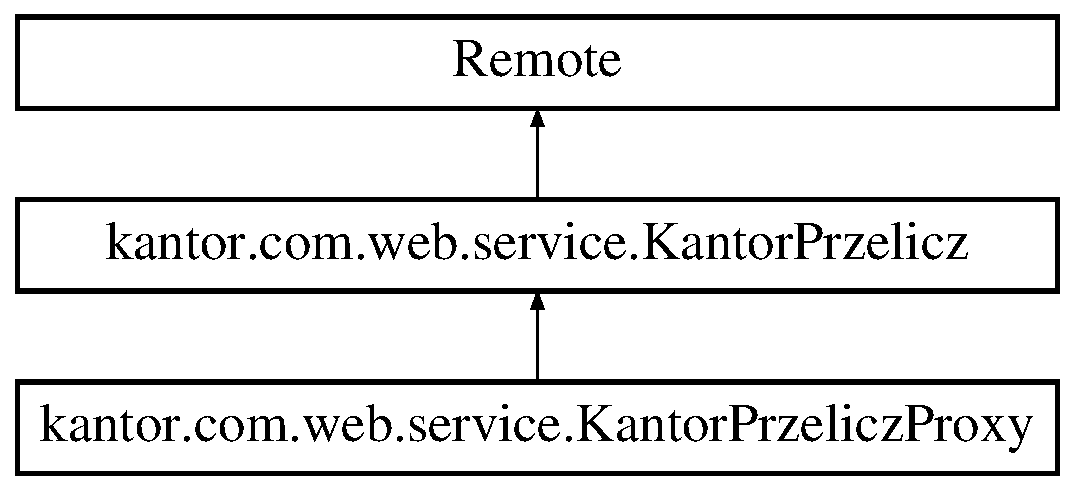
\includegraphics[height=3.000000cm]{classkantor_1_1com_1_1web_1_1service_1_1_kantor_przelicz_proxy}
\end{center}
\end{figure}
\subsection*{Public Member Functions}
\begin{DoxyCompactItemize}
\item 
\hyperlink{classkantor_1_1com_1_1web_1_1service_1_1_kantor_przelicz_proxy_a11a96bae697b462d20db8fbc8b0bdbd4}{Kantor\+Przelicz\+Proxy} ()
\item 
\hyperlink{classkantor_1_1com_1_1web_1_1service_1_1_kantor_przelicz_proxy_a2a4e73b8a9302c1747ba75be35655986}{Kantor\+Przelicz\+Proxy} (String endpoint)
\item 
String \hyperlink{classkantor_1_1com_1_1web_1_1service_1_1_kantor_przelicz_proxy_aa15f2063604ca099ee2135bdfd3ad0a3}{get\+Endpoint} ()
\item 
void \hyperlink{classkantor_1_1com_1_1web_1_1service_1_1_kantor_przelicz_proxy_a4634c8f62799df6b19a7724abcee8e05}{set\+Endpoint} (String endpoint)
\item 
\hyperlink{classkantor_1_1com_1_1web_1_1service_1_1_kantor_przelicz}{kantor.\+com.\+web.\+service.\+Kantor\+Przelicz} \hyperlink{classkantor_1_1com_1_1web_1_1service_1_1_kantor_przelicz_proxy_a8fa481638a7cb75bb43f49f824054fe8}{get\+Kantor\+Przelicz} ()
\item 
double\mbox{[}$\,$\mbox{]} \hyperlink{classkantor_1_1com_1_1web_1_1service_1_1_kantor_przelicz_proxy_a7fa719bb81dec0293285538a0e421580}{pobierz\+\_\+kursy\+\_\+walut} ()  throws java.\+rmi.\+Remote\+Exception
\item 
double \hyperlink{classkantor_1_1com_1_1web_1_1service_1_1_kantor_przelicz_proxy_a11fcb67da28afd357d34f545754a9738}{G\+B\+Pna\+P\+L\+N} (double value)  throws java.\+rmi.\+Remote\+Exception
\item 
double \hyperlink{classkantor_1_1com_1_1web_1_1service_1_1_kantor_przelicz_proxy_aa2add2cb979600a2b325e4a9f91b8e7f}{P\+L\+Nna\+R\+U\+B} (double value)  throws java.\+rmi.\+Remote\+Exception
\item 
double \hyperlink{classkantor_1_1com_1_1web_1_1service_1_1_kantor_przelicz_proxy_aa8471360bfae3c5acb208c2724971c8b}{J\+P\+Yna\+P\+L\+N} (double value)  throws java.\+rmi.\+Remote\+Exception
\item 
double \hyperlink{classkantor_1_1com_1_1web_1_1service_1_1_kantor_przelicz_proxy_a580df822a271928481e22b7c7d79bfec}{P\+L\+Nna\+G\+B\+P} (double value)  throws java.\+rmi.\+Remote\+Exception
\item 
double \hyperlink{classkantor_1_1com_1_1web_1_1service_1_1_kantor_przelicz_proxy_a81e31cce00a952fc8c0781291b4023af}{P\+L\+Nna\+J\+P\+Y} (double value)  throws java.\+rmi.\+Remote\+Exception
\item 
double \hyperlink{classkantor_1_1com_1_1web_1_1service_1_1_kantor_przelicz_proxy_a7c1eb7f1917e3f6f69b5d4c20f18a764}{R\+U\+Bna\+P\+L\+N} (double value)  throws java.\+rmi.\+Remote\+Exception
\item 
double \hyperlink{classkantor_1_1com_1_1web_1_1service_1_1_kantor_przelicz_proxy_ad6db21ad3720cdfaf5d27db59412c630}{U\+S\+Dna\+P\+L\+N} (double value)  throws java.\+rmi.\+Remote\+Exception
\item 
double \hyperlink{classkantor_1_1com_1_1web_1_1service_1_1_kantor_przelicz_proxy_a18431c0ee3b7a7765911cf055ff10cea}{P\+L\+Nna\+U\+S\+D} (double value)  throws java.\+rmi.\+Remote\+Exception
\item 
double \hyperlink{classkantor_1_1com_1_1web_1_1service_1_1_kantor_przelicz_proxy_afcaaed0493d9da86ff7eb4d6fb3a7e6d}{E\+U\+Rna\+P\+L\+N} (double value)  throws java.\+rmi.\+Remote\+Exception
\item 
double \hyperlink{classkantor_1_1com_1_1web_1_1service_1_1_kantor_przelicz_proxy_a4ee32718c9f24b212f904e46fbb734bf}{P\+L\+Nna\+E\+U\+R} (double value)  throws java.\+rmi.\+Remote\+Exception
\item 
double \hyperlink{classkantor_1_1com_1_1web_1_1service_1_1_kantor_przelicz_proxy_a2034d7a78dc86c2fbeb9c104c5ff04f1}{P\+L\+Nna\+C\+H\+E} (double value)  throws java.\+rmi.\+Remote\+Exception
\item 
double \hyperlink{classkantor_1_1com_1_1web_1_1service_1_1_kantor_przelicz_proxy_a3e40e9d8fb68c3edc8d0301b2fe524b6}{C\+H\+Ena\+P\+L\+N} (double value)  throws java.\+rmi.\+Remote\+Exception
\end{DoxyCompactItemize}


\subsection{Detailed Description}


Definition at line 3 of file Kantor\+Przelicz\+Proxy.\+java.



\subsection{Constructor \& Destructor Documentation}
\hypertarget{classkantor_1_1com_1_1web_1_1service_1_1_kantor_przelicz_proxy_a11a96bae697b462d20db8fbc8b0bdbd4}{\index{kantor\+::com\+::web\+::service\+::\+Kantor\+Przelicz\+Proxy@{kantor\+::com\+::web\+::service\+::\+Kantor\+Przelicz\+Proxy}!Kantor\+Przelicz\+Proxy@{Kantor\+Przelicz\+Proxy}}
\index{Kantor\+Przelicz\+Proxy@{Kantor\+Przelicz\+Proxy}!kantor\+::com\+::web\+::service\+::\+Kantor\+Przelicz\+Proxy@{kantor\+::com\+::web\+::service\+::\+Kantor\+Przelicz\+Proxy}}
\subsubsection[{Kantor\+Przelicz\+Proxy}]{\setlength{\rightskip}{0pt plus 5cm}kantor.\+com.\+web.\+service.\+Kantor\+Przelicz\+Proxy.\+Kantor\+Przelicz\+Proxy (
\begin{DoxyParamCaption}
{}
\end{DoxyParamCaption}
)}}\label{classkantor_1_1com_1_1web_1_1service_1_1_kantor_przelicz_proxy_a11a96bae697b462d20db8fbc8b0bdbd4}


Definition at line 7 of file Kantor\+Przelicz\+Proxy.\+java.

\hypertarget{classkantor_1_1com_1_1web_1_1service_1_1_kantor_przelicz_proxy_a2a4e73b8a9302c1747ba75be35655986}{\index{kantor\+::com\+::web\+::service\+::\+Kantor\+Przelicz\+Proxy@{kantor\+::com\+::web\+::service\+::\+Kantor\+Przelicz\+Proxy}!Kantor\+Przelicz\+Proxy@{Kantor\+Przelicz\+Proxy}}
\index{Kantor\+Przelicz\+Proxy@{Kantor\+Przelicz\+Proxy}!kantor\+::com\+::web\+::service\+::\+Kantor\+Przelicz\+Proxy@{kantor\+::com\+::web\+::service\+::\+Kantor\+Przelicz\+Proxy}}
\subsubsection[{Kantor\+Przelicz\+Proxy}]{\setlength{\rightskip}{0pt plus 5cm}kantor.\+com.\+web.\+service.\+Kantor\+Przelicz\+Proxy.\+Kantor\+Przelicz\+Proxy (
\begin{DoxyParamCaption}
\item[{String}]{endpoint}
\end{DoxyParamCaption}
)}}\label{classkantor_1_1com_1_1web_1_1service_1_1_kantor_przelicz_proxy_a2a4e73b8a9302c1747ba75be35655986}


Definition at line 11 of file Kantor\+Przelicz\+Proxy.\+java.



\subsection{Member Function Documentation}
\hypertarget{classkantor_1_1com_1_1web_1_1service_1_1_kantor_przelicz_proxy_a3e40e9d8fb68c3edc8d0301b2fe524b6}{\index{kantor\+::com\+::web\+::service\+::\+Kantor\+Przelicz\+Proxy@{kantor\+::com\+::web\+::service\+::\+Kantor\+Przelicz\+Proxy}!C\+H\+Ena\+P\+L\+N@{C\+H\+Ena\+P\+L\+N}}
\index{C\+H\+Ena\+P\+L\+N@{C\+H\+Ena\+P\+L\+N}!kantor\+::com\+::web\+::service\+::\+Kantor\+Przelicz\+Proxy@{kantor\+::com\+::web\+::service\+::\+Kantor\+Przelicz\+Proxy}}
\subsubsection[{C\+H\+Ena\+P\+L\+N}]{\setlength{\rightskip}{0pt plus 5cm}double kantor.\+com.\+web.\+service.\+Kantor\+Przelicz\+Proxy.\+C\+H\+Ena\+P\+L\+N (
\begin{DoxyParamCaption}
\item[{double}]{value}
\end{DoxyParamCaption}
) throws java.\+rmi.\+Remote\+Exception}}\label{classkantor_1_1com_1_1web_1_1service_1_1_kantor_przelicz_proxy_a3e40e9d8fb68c3edc8d0301b2fe524b6}


Implements \hyperlink{classkantor_1_1com_1_1web_1_1service_1_1_kantor_przelicz_acff8492d50d84cf718bca4c8b499d36a}{kantor.\+com.\+web.\+service.\+Kantor\+Przelicz}.



Definition at line 119 of file Kantor\+Przelicz\+Proxy.\+java.

\hypertarget{classkantor_1_1com_1_1web_1_1service_1_1_kantor_przelicz_proxy_afcaaed0493d9da86ff7eb4d6fb3a7e6d}{\index{kantor\+::com\+::web\+::service\+::\+Kantor\+Przelicz\+Proxy@{kantor\+::com\+::web\+::service\+::\+Kantor\+Przelicz\+Proxy}!E\+U\+Rna\+P\+L\+N@{E\+U\+Rna\+P\+L\+N}}
\index{E\+U\+Rna\+P\+L\+N@{E\+U\+Rna\+P\+L\+N}!kantor\+::com\+::web\+::service\+::\+Kantor\+Przelicz\+Proxy@{kantor\+::com\+::web\+::service\+::\+Kantor\+Przelicz\+Proxy}}
\subsubsection[{E\+U\+Rna\+P\+L\+N}]{\setlength{\rightskip}{0pt plus 5cm}double kantor.\+com.\+web.\+service.\+Kantor\+Przelicz\+Proxy.\+E\+U\+Rna\+P\+L\+N (
\begin{DoxyParamCaption}
\item[{double}]{value}
\end{DoxyParamCaption}
) throws java.\+rmi.\+Remote\+Exception}}\label{classkantor_1_1com_1_1web_1_1service_1_1_kantor_przelicz_proxy_afcaaed0493d9da86ff7eb4d6fb3a7e6d}


Implements \hyperlink{classkantor_1_1com_1_1web_1_1service_1_1_kantor_przelicz_af204b150c62165c836a1a0afd10c16b7}{kantor.\+com.\+web.\+service.\+Kantor\+Przelicz}.



Definition at line 101 of file Kantor\+Przelicz\+Proxy.\+java.

\hypertarget{classkantor_1_1com_1_1web_1_1service_1_1_kantor_przelicz_proxy_a11fcb67da28afd357d34f545754a9738}{\index{kantor\+::com\+::web\+::service\+::\+Kantor\+Przelicz\+Proxy@{kantor\+::com\+::web\+::service\+::\+Kantor\+Przelicz\+Proxy}!G\+B\+Pna\+P\+L\+N@{G\+B\+Pna\+P\+L\+N}}
\index{G\+B\+Pna\+P\+L\+N@{G\+B\+Pna\+P\+L\+N}!kantor\+::com\+::web\+::service\+::\+Kantor\+Przelicz\+Proxy@{kantor\+::com\+::web\+::service\+::\+Kantor\+Przelicz\+Proxy}}
\subsubsection[{G\+B\+Pna\+P\+L\+N}]{\setlength{\rightskip}{0pt plus 5cm}double kantor.\+com.\+web.\+service.\+Kantor\+Przelicz\+Proxy.\+G\+B\+Pna\+P\+L\+N (
\begin{DoxyParamCaption}
\item[{double}]{value}
\end{DoxyParamCaption}
) throws java.\+rmi.\+Remote\+Exception}}\label{classkantor_1_1com_1_1web_1_1service_1_1_kantor_przelicz_proxy_a11fcb67da28afd357d34f545754a9738}


Implements \hyperlink{classkantor_1_1com_1_1web_1_1service_1_1_kantor_przelicz_a64b58db5e686a08b4b1af648eb781a1c}{kantor.\+com.\+web.\+service.\+Kantor\+Przelicz}.



Definition at line 53 of file Kantor\+Przelicz\+Proxy.\+java.

\hypertarget{classkantor_1_1com_1_1web_1_1service_1_1_kantor_przelicz_proxy_aa15f2063604ca099ee2135bdfd3ad0a3}{\index{kantor\+::com\+::web\+::service\+::\+Kantor\+Przelicz\+Proxy@{kantor\+::com\+::web\+::service\+::\+Kantor\+Przelicz\+Proxy}!get\+Endpoint@{get\+Endpoint}}
\index{get\+Endpoint@{get\+Endpoint}!kantor\+::com\+::web\+::service\+::\+Kantor\+Przelicz\+Proxy@{kantor\+::com\+::web\+::service\+::\+Kantor\+Przelicz\+Proxy}}
\subsubsection[{get\+Endpoint}]{\setlength{\rightskip}{0pt plus 5cm}String kantor.\+com.\+web.\+service.\+Kantor\+Przelicz\+Proxy.\+get\+Endpoint (
\begin{DoxyParamCaption}
{}
\end{DoxyParamCaption}
)}}\label{classkantor_1_1com_1_1web_1_1service_1_1_kantor_przelicz_proxy_aa15f2063604ca099ee2135bdfd3ad0a3}


Definition at line 30 of file Kantor\+Przelicz\+Proxy.\+java.

\hypertarget{classkantor_1_1com_1_1web_1_1service_1_1_kantor_przelicz_proxy_a8fa481638a7cb75bb43f49f824054fe8}{\index{kantor\+::com\+::web\+::service\+::\+Kantor\+Przelicz\+Proxy@{kantor\+::com\+::web\+::service\+::\+Kantor\+Przelicz\+Proxy}!get\+Kantor\+Przelicz@{get\+Kantor\+Przelicz}}
\index{get\+Kantor\+Przelicz@{get\+Kantor\+Przelicz}!kantor\+::com\+::web\+::service\+::\+Kantor\+Przelicz\+Proxy@{kantor\+::com\+::web\+::service\+::\+Kantor\+Przelicz\+Proxy}}
\subsubsection[{get\+Kantor\+Przelicz}]{\setlength{\rightskip}{0pt plus 5cm}{\bf kantor.\+com.\+web.\+service.\+Kantor\+Przelicz} kantor.\+com.\+web.\+service.\+Kantor\+Przelicz\+Proxy.\+get\+Kantor\+Przelicz (
\begin{DoxyParamCaption}
{}
\end{DoxyParamCaption}
)}}\label{classkantor_1_1com_1_1web_1_1service_1_1_kantor_przelicz_proxy_a8fa481638a7cb75bb43f49f824054fe8}


Definition at line 41 of file Kantor\+Przelicz\+Proxy.\+java.

\hypertarget{classkantor_1_1com_1_1web_1_1service_1_1_kantor_przelicz_proxy_aa8471360bfae3c5acb208c2724971c8b}{\index{kantor\+::com\+::web\+::service\+::\+Kantor\+Przelicz\+Proxy@{kantor\+::com\+::web\+::service\+::\+Kantor\+Przelicz\+Proxy}!J\+P\+Yna\+P\+L\+N@{J\+P\+Yna\+P\+L\+N}}
\index{J\+P\+Yna\+P\+L\+N@{J\+P\+Yna\+P\+L\+N}!kantor\+::com\+::web\+::service\+::\+Kantor\+Przelicz\+Proxy@{kantor\+::com\+::web\+::service\+::\+Kantor\+Przelicz\+Proxy}}
\subsubsection[{J\+P\+Yna\+P\+L\+N}]{\setlength{\rightskip}{0pt plus 5cm}double kantor.\+com.\+web.\+service.\+Kantor\+Przelicz\+Proxy.\+J\+P\+Yna\+P\+L\+N (
\begin{DoxyParamCaption}
\item[{double}]{value}
\end{DoxyParamCaption}
) throws java.\+rmi.\+Remote\+Exception}}\label{classkantor_1_1com_1_1web_1_1service_1_1_kantor_przelicz_proxy_aa8471360bfae3c5acb208c2724971c8b}


Implements \hyperlink{classkantor_1_1com_1_1web_1_1service_1_1_kantor_przelicz_a9e6f2e71874e1dd7b520d2da4427bae8}{kantor.\+com.\+web.\+service.\+Kantor\+Przelicz}.



Definition at line 65 of file Kantor\+Przelicz\+Proxy.\+java.

\hypertarget{classkantor_1_1com_1_1web_1_1service_1_1_kantor_przelicz_proxy_a2034d7a78dc86c2fbeb9c104c5ff04f1}{\index{kantor\+::com\+::web\+::service\+::\+Kantor\+Przelicz\+Proxy@{kantor\+::com\+::web\+::service\+::\+Kantor\+Przelicz\+Proxy}!P\+L\+Nna\+C\+H\+E@{P\+L\+Nna\+C\+H\+E}}
\index{P\+L\+Nna\+C\+H\+E@{P\+L\+Nna\+C\+H\+E}!kantor\+::com\+::web\+::service\+::\+Kantor\+Przelicz\+Proxy@{kantor\+::com\+::web\+::service\+::\+Kantor\+Przelicz\+Proxy}}
\subsubsection[{P\+L\+Nna\+C\+H\+E}]{\setlength{\rightskip}{0pt plus 5cm}double kantor.\+com.\+web.\+service.\+Kantor\+Przelicz\+Proxy.\+P\+L\+Nna\+C\+H\+E (
\begin{DoxyParamCaption}
\item[{double}]{value}
\end{DoxyParamCaption}
) throws java.\+rmi.\+Remote\+Exception}}\label{classkantor_1_1com_1_1web_1_1service_1_1_kantor_przelicz_proxy_a2034d7a78dc86c2fbeb9c104c5ff04f1}


Implements \hyperlink{classkantor_1_1com_1_1web_1_1service_1_1_kantor_przelicz_afa953802446690d409e1df5361729fc0}{kantor.\+com.\+web.\+service.\+Kantor\+Przelicz}.



Definition at line 113 of file Kantor\+Przelicz\+Proxy.\+java.

\hypertarget{classkantor_1_1com_1_1web_1_1service_1_1_kantor_przelicz_proxy_a4ee32718c9f24b212f904e46fbb734bf}{\index{kantor\+::com\+::web\+::service\+::\+Kantor\+Przelicz\+Proxy@{kantor\+::com\+::web\+::service\+::\+Kantor\+Przelicz\+Proxy}!P\+L\+Nna\+E\+U\+R@{P\+L\+Nna\+E\+U\+R}}
\index{P\+L\+Nna\+E\+U\+R@{P\+L\+Nna\+E\+U\+R}!kantor\+::com\+::web\+::service\+::\+Kantor\+Przelicz\+Proxy@{kantor\+::com\+::web\+::service\+::\+Kantor\+Przelicz\+Proxy}}
\subsubsection[{P\+L\+Nna\+E\+U\+R}]{\setlength{\rightskip}{0pt plus 5cm}double kantor.\+com.\+web.\+service.\+Kantor\+Przelicz\+Proxy.\+P\+L\+Nna\+E\+U\+R (
\begin{DoxyParamCaption}
\item[{double}]{value}
\end{DoxyParamCaption}
) throws java.\+rmi.\+Remote\+Exception}}\label{classkantor_1_1com_1_1web_1_1service_1_1_kantor_przelicz_proxy_a4ee32718c9f24b212f904e46fbb734bf}


Implements \hyperlink{classkantor_1_1com_1_1web_1_1service_1_1_kantor_przelicz_acfc0cd42fb64c5f26d468245cf0fe3b6}{kantor.\+com.\+web.\+service.\+Kantor\+Przelicz}.



Definition at line 107 of file Kantor\+Przelicz\+Proxy.\+java.

\hypertarget{classkantor_1_1com_1_1web_1_1service_1_1_kantor_przelicz_proxy_a580df822a271928481e22b7c7d79bfec}{\index{kantor\+::com\+::web\+::service\+::\+Kantor\+Przelicz\+Proxy@{kantor\+::com\+::web\+::service\+::\+Kantor\+Przelicz\+Proxy}!P\+L\+Nna\+G\+B\+P@{P\+L\+Nna\+G\+B\+P}}
\index{P\+L\+Nna\+G\+B\+P@{P\+L\+Nna\+G\+B\+P}!kantor\+::com\+::web\+::service\+::\+Kantor\+Przelicz\+Proxy@{kantor\+::com\+::web\+::service\+::\+Kantor\+Przelicz\+Proxy}}
\subsubsection[{P\+L\+Nna\+G\+B\+P}]{\setlength{\rightskip}{0pt plus 5cm}double kantor.\+com.\+web.\+service.\+Kantor\+Przelicz\+Proxy.\+P\+L\+Nna\+G\+B\+P (
\begin{DoxyParamCaption}
\item[{double}]{value}
\end{DoxyParamCaption}
) throws java.\+rmi.\+Remote\+Exception}}\label{classkantor_1_1com_1_1web_1_1service_1_1_kantor_przelicz_proxy_a580df822a271928481e22b7c7d79bfec}


Implements \hyperlink{classkantor_1_1com_1_1web_1_1service_1_1_kantor_przelicz_ad0840077798f333f948772590d1a402a}{kantor.\+com.\+web.\+service.\+Kantor\+Przelicz}.



Definition at line 71 of file Kantor\+Przelicz\+Proxy.\+java.

\hypertarget{classkantor_1_1com_1_1web_1_1service_1_1_kantor_przelicz_proxy_a81e31cce00a952fc8c0781291b4023af}{\index{kantor\+::com\+::web\+::service\+::\+Kantor\+Przelicz\+Proxy@{kantor\+::com\+::web\+::service\+::\+Kantor\+Przelicz\+Proxy}!P\+L\+Nna\+J\+P\+Y@{P\+L\+Nna\+J\+P\+Y}}
\index{P\+L\+Nna\+J\+P\+Y@{P\+L\+Nna\+J\+P\+Y}!kantor\+::com\+::web\+::service\+::\+Kantor\+Przelicz\+Proxy@{kantor\+::com\+::web\+::service\+::\+Kantor\+Przelicz\+Proxy}}
\subsubsection[{P\+L\+Nna\+J\+P\+Y}]{\setlength{\rightskip}{0pt plus 5cm}double kantor.\+com.\+web.\+service.\+Kantor\+Przelicz\+Proxy.\+P\+L\+Nna\+J\+P\+Y (
\begin{DoxyParamCaption}
\item[{double}]{value}
\end{DoxyParamCaption}
) throws java.\+rmi.\+Remote\+Exception}}\label{classkantor_1_1com_1_1web_1_1service_1_1_kantor_przelicz_proxy_a81e31cce00a952fc8c0781291b4023af}


Implements \hyperlink{classkantor_1_1com_1_1web_1_1service_1_1_kantor_przelicz_a7706e3a08c1b8ce3775506c4530d1bf7}{kantor.\+com.\+web.\+service.\+Kantor\+Przelicz}.



Definition at line 77 of file Kantor\+Przelicz\+Proxy.\+java.

\hypertarget{classkantor_1_1com_1_1web_1_1service_1_1_kantor_przelicz_proxy_aa2add2cb979600a2b325e4a9f91b8e7f}{\index{kantor\+::com\+::web\+::service\+::\+Kantor\+Przelicz\+Proxy@{kantor\+::com\+::web\+::service\+::\+Kantor\+Przelicz\+Proxy}!P\+L\+Nna\+R\+U\+B@{P\+L\+Nna\+R\+U\+B}}
\index{P\+L\+Nna\+R\+U\+B@{P\+L\+Nna\+R\+U\+B}!kantor\+::com\+::web\+::service\+::\+Kantor\+Przelicz\+Proxy@{kantor\+::com\+::web\+::service\+::\+Kantor\+Przelicz\+Proxy}}
\subsubsection[{P\+L\+Nna\+R\+U\+B}]{\setlength{\rightskip}{0pt plus 5cm}double kantor.\+com.\+web.\+service.\+Kantor\+Przelicz\+Proxy.\+P\+L\+Nna\+R\+U\+B (
\begin{DoxyParamCaption}
\item[{double}]{value}
\end{DoxyParamCaption}
) throws java.\+rmi.\+Remote\+Exception}}\label{classkantor_1_1com_1_1web_1_1service_1_1_kantor_przelicz_proxy_aa2add2cb979600a2b325e4a9f91b8e7f}


Implements \hyperlink{classkantor_1_1com_1_1web_1_1service_1_1_kantor_przelicz_ad68cbeb18f18cd02c3b4b571da0e06fa}{kantor.\+com.\+web.\+service.\+Kantor\+Przelicz}.



Definition at line 59 of file Kantor\+Przelicz\+Proxy.\+java.

\hypertarget{classkantor_1_1com_1_1web_1_1service_1_1_kantor_przelicz_proxy_a18431c0ee3b7a7765911cf055ff10cea}{\index{kantor\+::com\+::web\+::service\+::\+Kantor\+Przelicz\+Proxy@{kantor\+::com\+::web\+::service\+::\+Kantor\+Przelicz\+Proxy}!P\+L\+Nna\+U\+S\+D@{P\+L\+Nna\+U\+S\+D}}
\index{P\+L\+Nna\+U\+S\+D@{P\+L\+Nna\+U\+S\+D}!kantor\+::com\+::web\+::service\+::\+Kantor\+Przelicz\+Proxy@{kantor\+::com\+::web\+::service\+::\+Kantor\+Przelicz\+Proxy}}
\subsubsection[{P\+L\+Nna\+U\+S\+D}]{\setlength{\rightskip}{0pt plus 5cm}double kantor.\+com.\+web.\+service.\+Kantor\+Przelicz\+Proxy.\+P\+L\+Nna\+U\+S\+D (
\begin{DoxyParamCaption}
\item[{double}]{value}
\end{DoxyParamCaption}
) throws java.\+rmi.\+Remote\+Exception}}\label{classkantor_1_1com_1_1web_1_1service_1_1_kantor_przelicz_proxy_a18431c0ee3b7a7765911cf055ff10cea}


Implements \hyperlink{classkantor_1_1com_1_1web_1_1service_1_1_kantor_przelicz_aea3a5dd74cf10d0c9ce1bf04b94078c8}{kantor.\+com.\+web.\+service.\+Kantor\+Przelicz}.



Definition at line 95 of file Kantor\+Przelicz\+Proxy.\+java.

\hypertarget{classkantor_1_1com_1_1web_1_1service_1_1_kantor_przelicz_proxy_a7fa719bb81dec0293285538a0e421580}{\index{kantor\+::com\+::web\+::service\+::\+Kantor\+Przelicz\+Proxy@{kantor\+::com\+::web\+::service\+::\+Kantor\+Przelicz\+Proxy}!pobierz\+\_\+kursy\+\_\+walut@{pobierz\+\_\+kursy\+\_\+walut}}
\index{pobierz\+\_\+kursy\+\_\+walut@{pobierz\+\_\+kursy\+\_\+walut}!kantor\+::com\+::web\+::service\+::\+Kantor\+Przelicz\+Proxy@{kantor\+::com\+::web\+::service\+::\+Kantor\+Przelicz\+Proxy}}
\subsubsection[{pobierz\+\_\+kursy\+\_\+walut}]{\setlength{\rightskip}{0pt plus 5cm}double \mbox{[}$\,$\mbox{]} kantor.\+com.\+web.\+service.\+Kantor\+Przelicz\+Proxy.\+pobierz\+\_\+kursy\+\_\+walut (
\begin{DoxyParamCaption}
{}
\end{DoxyParamCaption}
) throws java.\+rmi.\+Remote\+Exception}}\label{classkantor_1_1com_1_1web_1_1service_1_1_kantor_przelicz_proxy_a7fa719bb81dec0293285538a0e421580}


Implements \hyperlink{classkantor_1_1com_1_1web_1_1service_1_1_kantor_przelicz_a9e2610a2cdb76ea7e2551786f3c0736e}{kantor.\+com.\+web.\+service.\+Kantor\+Przelicz}.



Definition at line 47 of file Kantor\+Przelicz\+Proxy.\+java.

\hypertarget{classkantor_1_1com_1_1web_1_1service_1_1_kantor_przelicz_proxy_a7c1eb7f1917e3f6f69b5d4c20f18a764}{\index{kantor\+::com\+::web\+::service\+::\+Kantor\+Przelicz\+Proxy@{kantor\+::com\+::web\+::service\+::\+Kantor\+Przelicz\+Proxy}!R\+U\+Bna\+P\+L\+N@{R\+U\+Bna\+P\+L\+N}}
\index{R\+U\+Bna\+P\+L\+N@{R\+U\+Bna\+P\+L\+N}!kantor\+::com\+::web\+::service\+::\+Kantor\+Przelicz\+Proxy@{kantor\+::com\+::web\+::service\+::\+Kantor\+Przelicz\+Proxy}}
\subsubsection[{R\+U\+Bna\+P\+L\+N}]{\setlength{\rightskip}{0pt plus 5cm}double kantor.\+com.\+web.\+service.\+Kantor\+Przelicz\+Proxy.\+R\+U\+Bna\+P\+L\+N (
\begin{DoxyParamCaption}
\item[{double}]{value}
\end{DoxyParamCaption}
) throws java.\+rmi.\+Remote\+Exception}}\label{classkantor_1_1com_1_1web_1_1service_1_1_kantor_przelicz_proxy_a7c1eb7f1917e3f6f69b5d4c20f18a764}


Implements \hyperlink{classkantor_1_1com_1_1web_1_1service_1_1_kantor_przelicz_a11c3958baf84a3a96dbc9290890b6c4e}{kantor.\+com.\+web.\+service.\+Kantor\+Przelicz}.



Definition at line 83 of file Kantor\+Przelicz\+Proxy.\+java.

\hypertarget{classkantor_1_1com_1_1web_1_1service_1_1_kantor_przelicz_proxy_a4634c8f62799df6b19a7724abcee8e05}{\index{kantor\+::com\+::web\+::service\+::\+Kantor\+Przelicz\+Proxy@{kantor\+::com\+::web\+::service\+::\+Kantor\+Przelicz\+Proxy}!set\+Endpoint@{set\+Endpoint}}
\index{set\+Endpoint@{set\+Endpoint}!kantor\+::com\+::web\+::service\+::\+Kantor\+Przelicz\+Proxy@{kantor\+::com\+::web\+::service\+::\+Kantor\+Przelicz\+Proxy}}
\subsubsection[{set\+Endpoint}]{\setlength{\rightskip}{0pt plus 5cm}void kantor.\+com.\+web.\+service.\+Kantor\+Przelicz\+Proxy.\+set\+Endpoint (
\begin{DoxyParamCaption}
\item[{String}]{endpoint}
\end{DoxyParamCaption}
)}}\label{classkantor_1_1com_1_1web_1_1service_1_1_kantor_przelicz_proxy_a4634c8f62799df6b19a7724abcee8e05}


Definition at line 34 of file Kantor\+Przelicz\+Proxy.\+java.

\hypertarget{classkantor_1_1com_1_1web_1_1service_1_1_kantor_przelicz_proxy_ad6db21ad3720cdfaf5d27db59412c630}{\index{kantor\+::com\+::web\+::service\+::\+Kantor\+Przelicz\+Proxy@{kantor\+::com\+::web\+::service\+::\+Kantor\+Przelicz\+Proxy}!U\+S\+Dna\+P\+L\+N@{U\+S\+Dna\+P\+L\+N}}
\index{U\+S\+Dna\+P\+L\+N@{U\+S\+Dna\+P\+L\+N}!kantor\+::com\+::web\+::service\+::\+Kantor\+Przelicz\+Proxy@{kantor\+::com\+::web\+::service\+::\+Kantor\+Przelicz\+Proxy}}
\subsubsection[{U\+S\+Dna\+P\+L\+N}]{\setlength{\rightskip}{0pt plus 5cm}double kantor.\+com.\+web.\+service.\+Kantor\+Przelicz\+Proxy.\+U\+S\+Dna\+P\+L\+N (
\begin{DoxyParamCaption}
\item[{double}]{value}
\end{DoxyParamCaption}
) throws java.\+rmi.\+Remote\+Exception}}\label{classkantor_1_1com_1_1web_1_1service_1_1_kantor_przelicz_proxy_ad6db21ad3720cdfaf5d27db59412c630}


Implements \hyperlink{classkantor_1_1com_1_1web_1_1service_1_1_kantor_przelicz_ad263683559db773d4ccb28e14090824f}{kantor.\+com.\+web.\+service.\+Kantor\+Przelicz}.



Definition at line 89 of file Kantor\+Przelicz\+Proxy.\+java.



The documentation for this class was generated from the following file\+:\begin{DoxyCompactItemize}
\item 
C\+:/\+Users/kuska/\+Desktop/\+Michalik/\+K\+W/\+Kantor\+W\+S\+Client/src/kantor/com/web/service/\hyperlink{_kantor_przelicz_proxy_8java}{Kantor\+Przelicz\+Proxy.\+java}\end{DoxyCompactItemize}

\hypertarget{interfacekantor_1_1com_1_1web_1_1service_1_1_kantor_przelicz_service}{\section{kantor.\+com.\+web.\+service.\+Kantor\+Przelicz\+Service Interface Reference}
\label{interfacekantor_1_1com_1_1web_1_1service_1_1_kantor_przelicz_service}\index{kantor.\+com.\+web.\+service.\+Kantor\+Przelicz\+Service@{kantor.\+com.\+web.\+service.\+Kantor\+Przelicz\+Service}}
}
Inheritance diagram for kantor.\+com.\+web.\+service.\+Kantor\+Przelicz\+Service\+:\begin{figure}[H]
\begin{center}
\leavevmode
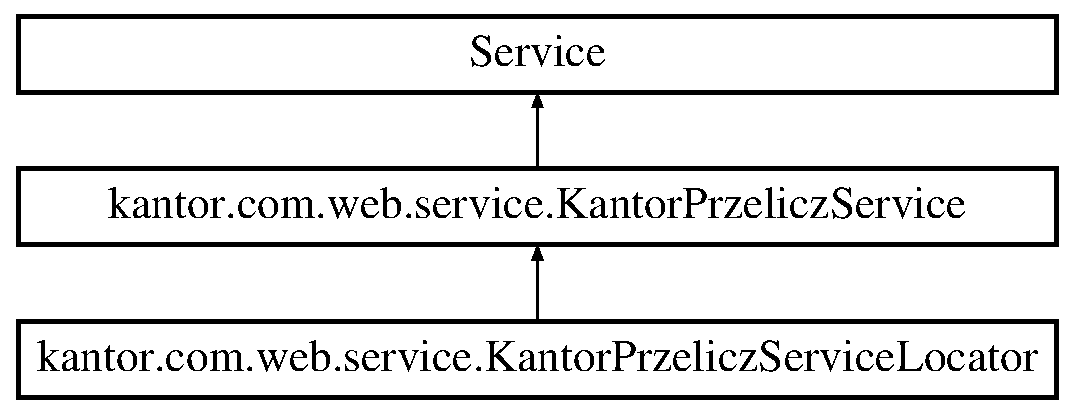
\includegraphics[height=3.000000cm]{interfacekantor_1_1com_1_1web_1_1service_1_1_kantor_przelicz_service}
\end{center}
\end{figure}
\subsection*{Public Member Functions}
\begin{DoxyCompactItemize}
\item 
java.\+lang.\+String \hyperlink{interfacekantor_1_1com_1_1web_1_1service_1_1_kantor_przelicz_service_a6e8a852eedd0efb826c9b7fba061e577}{get\+Kantor\+Przelicz\+Address} ()
\item 
\hyperlink{classkantor_1_1com_1_1web_1_1service_1_1_kantor_przelicz}{kantor.\+com.\+web.\+service.\+Kantor\+Przelicz} \hyperlink{interfacekantor_1_1com_1_1web_1_1service_1_1_kantor_przelicz_service_a23dc3e9c5f8aaeb4d50a1e8b6f51677b}{get\+Kantor\+Przelicz} ()  throws javax.\+xml.\+rpc.\+Service\+Exception
\item 
\hyperlink{classkantor_1_1com_1_1web_1_1service_1_1_kantor_przelicz}{kantor.\+com.\+web.\+service.\+Kantor\+Przelicz} \hyperlink{interfacekantor_1_1com_1_1web_1_1service_1_1_kantor_przelicz_service_a3c33e0adf664558840bd2e1b1d9da37d}{get\+Kantor\+Przelicz} (java.\+net.\+U\+R\+L port\+Address)  throws javax.\+xml.\+rpc.\+Service\+Exception
\end{DoxyCompactItemize}


\subsection{Detailed Description}


Definition at line 10 of file Kantor\+Przelicz\+Service.\+java.



\subsection{Member Function Documentation}
\hypertarget{interfacekantor_1_1com_1_1web_1_1service_1_1_kantor_przelicz_service_a23dc3e9c5f8aaeb4d50a1e8b6f51677b}{\index{kantor\+::com\+::web\+::service\+::\+Kantor\+Przelicz\+Service@{kantor\+::com\+::web\+::service\+::\+Kantor\+Przelicz\+Service}!get\+Kantor\+Przelicz@{get\+Kantor\+Przelicz}}
\index{get\+Kantor\+Przelicz@{get\+Kantor\+Przelicz}!kantor\+::com\+::web\+::service\+::\+Kantor\+Przelicz\+Service@{kantor\+::com\+::web\+::service\+::\+Kantor\+Przelicz\+Service}}
\subsubsection[{get\+Kantor\+Przelicz}]{\setlength{\rightskip}{0pt plus 5cm}{\bf kantor.\+com.\+web.\+service.\+Kantor\+Przelicz} kantor.\+com.\+web.\+service.\+Kantor\+Przelicz\+Service.\+get\+Kantor\+Przelicz (
\begin{DoxyParamCaption}
{}
\end{DoxyParamCaption}
) throws javax.\+xml.\+rpc.\+Service\+Exception}}\label{interfacekantor_1_1com_1_1web_1_1service_1_1_kantor_przelicz_service_a23dc3e9c5f8aaeb4d50a1e8b6f51677b}


Implemented in \hyperlink{classkantor_1_1com_1_1web_1_1service_1_1_kantor_przelicz_service_locator_a3844af66601dcdb811a31551ce63df11}{kantor.\+com.\+web.\+service.\+Kantor\+Przelicz\+Service\+Locator}.

\hypertarget{interfacekantor_1_1com_1_1web_1_1service_1_1_kantor_przelicz_service_a3c33e0adf664558840bd2e1b1d9da37d}{\index{kantor\+::com\+::web\+::service\+::\+Kantor\+Przelicz\+Service@{kantor\+::com\+::web\+::service\+::\+Kantor\+Przelicz\+Service}!get\+Kantor\+Przelicz@{get\+Kantor\+Przelicz}}
\index{get\+Kantor\+Przelicz@{get\+Kantor\+Przelicz}!kantor\+::com\+::web\+::service\+::\+Kantor\+Przelicz\+Service@{kantor\+::com\+::web\+::service\+::\+Kantor\+Przelicz\+Service}}
\subsubsection[{get\+Kantor\+Przelicz}]{\setlength{\rightskip}{0pt plus 5cm}{\bf kantor.\+com.\+web.\+service.\+Kantor\+Przelicz} kantor.\+com.\+web.\+service.\+Kantor\+Przelicz\+Service.\+get\+Kantor\+Przelicz (
\begin{DoxyParamCaption}
\item[{java.\+net.\+U\+R\+L}]{port\+Address}
\end{DoxyParamCaption}
) throws javax.\+xml.\+rpc.\+Service\+Exception}}\label{interfacekantor_1_1com_1_1web_1_1service_1_1_kantor_przelicz_service_a3c33e0adf664558840bd2e1b1d9da37d}


Implemented in \hyperlink{classkantor_1_1com_1_1web_1_1service_1_1_kantor_przelicz_service_locator_afc2877ff5ca919546dea693a43df2d94}{kantor.\+com.\+web.\+service.\+Kantor\+Przelicz\+Service\+Locator}.

\hypertarget{interfacekantor_1_1com_1_1web_1_1service_1_1_kantor_przelicz_service_a6e8a852eedd0efb826c9b7fba061e577}{\index{kantor\+::com\+::web\+::service\+::\+Kantor\+Przelicz\+Service@{kantor\+::com\+::web\+::service\+::\+Kantor\+Przelicz\+Service}!get\+Kantor\+Przelicz\+Address@{get\+Kantor\+Przelicz\+Address}}
\index{get\+Kantor\+Przelicz\+Address@{get\+Kantor\+Przelicz\+Address}!kantor\+::com\+::web\+::service\+::\+Kantor\+Przelicz\+Service@{kantor\+::com\+::web\+::service\+::\+Kantor\+Przelicz\+Service}}
\subsubsection[{get\+Kantor\+Przelicz\+Address}]{\setlength{\rightskip}{0pt plus 5cm}java.\+lang.\+String kantor.\+com.\+web.\+service.\+Kantor\+Przelicz\+Service.\+get\+Kantor\+Przelicz\+Address (
\begin{DoxyParamCaption}
{}
\end{DoxyParamCaption}
)}}\label{interfacekantor_1_1com_1_1web_1_1service_1_1_kantor_przelicz_service_a6e8a852eedd0efb826c9b7fba061e577}


Implemented in \hyperlink{classkantor_1_1com_1_1web_1_1service_1_1_kantor_przelicz_service_locator_ac494431b6e486df99db8107de4eca1a3}{kantor.\+com.\+web.\+service.\+Kantor\+Przelicz\+Service\+Locator}.



The documentation for this interface was generated from the following file\+:\begin{DoxyCompactItemize}
\item 
C\+:/\+Users/kuska/\+Desktop/\+Michalik/\+K\+W/\+Kantor\+W\+S\+Client/src/kantor/com/web/service/\hyperlink{_kantor_przelicz_service_8java}{Kantor\+Przelicz\+Service.\+java}\end{DoxyCompactItemize}

\hypertarget{classkantor_1_1com_1_1web_1_1service_1_1_kantor_przelicz_service_locator}{\section{kantor.\+com.\+web.\+service.\+Kantor\+Przelicz\+Service\+Locator Class Reference}
\label{classkantor_1_1com_1_1web_1_1service_1_1_kantor_przelicz_service_locator}\index{kantor.\+com.\+web.\+service.\+Kantor\+Przelicz\+Service\+Locator@{kantor.\+com.\+web.\+service.\+Kantor\+Przelicz\+Service\+Locator}}
}
Inheritance diagram for kantor.\+com.\+web.\+service.\+Kantor\+Przelicz\+Service\+Locator\+:\begin{figure}[H]
\begin{center}
\leavevmode

\includegraphics[height=2.560976cm]{classkantor_1_1com_1_1web_1_1service_1_1_kantor_przelicz_service_locator}
\end{center}
\end{figure}
\subsection*{Public Member Functions}
\begin{DoxyCompactItemize}
\item 
\hyperlink{classkantor_1_1com_1_1web_1_1service_1_1_kantor_przelicz_service_locator_a1daad1d7591d70469d27d2a17a23bbb7}{Kantor\+Przelicz\+Service\+Locator} ()
\item 
\hyperlink{classkantor_1_1com_1_1web_1_1service_1_1_kantor_przelicz_service_locator_a86b910ad4c4d10b13597322aac38493c}{Kantor\+Przelicz\+Service\+Locator} (org.\+apache.\+axis.\+Engine\+Configuration config)
\item 
\hyperlink{classkantor_1_1com_1_1web_1_1service_1_1_kantor_przelicz_service_locator_a7803c401349057b4dc9464bee871fef9}{Kantor\+Przelicz\+Service\+Locator} (java.\+lang.\+String wsdl\+Loc, javax.\+xml.\+namespace.\+Q\+Name s\+Name)  throws javax.\+xml.\+rpc.\+Service\+Exception 
\item 
java.\+lang.\+String \hyperlink{classkantor_1_1com_1_1web_1_1service_1_1_kantor_przelicz_service_locator_ac494431b6e486df99db8107de4eca1a3}{get\+Kantor\+Przelicz\+Address} ()
\item 
java.\+lang.\+String \hyperlink{classkantor_1_1com_1_1web_1_1service_1_1_kantor_przelicz_service_locator_a66dc7bbfd82ca24ca18cffd72885ba6d}{get\+Kantor\+Przelicz\+W\+S\+D\+D\+Service\+Name} ()
\item 
void \hyperlink{classkantor_1_1com_1_1web_1_1service_1_1_kantor_przelicz_service_locator_a66de37b1b0144707a5f1622624de454f}{set\+Kantor\+Przelicz\+W\+S\+D\+D\+Service\+Name} (java.\+lang.\+String name)
\item 
\hyperlink{classkantor_1_1com_1_1web_1_1service_1_1_kantor_przelicz}{kantor.\+com.\+web.\+service.\+Kantor\+Przelicz} \hyperlink{classkantor_1_1com_1_1web_1_1service_1_1_kantor_przelicz_service_locator_a3844af66601dcdb811a31551ce63df11}{get\+Kantor\+Przelicz} ()  throws javax.\+xml.\+rpc.\+Service\+Exception 
\item 
\hyperlink{classkantor_1_1com_1_1web_1_1service_1_1_kantor_przelicz}{kantor.\+com.\+web.\+service.\+Kantor\+Przelicz} \hyperlink{classkantor_1_1com_1_1web_1_1service_1_1_kantor_przelicz_service_locator_afc2877ff5ca919546dea693a43df2d94}{get\+Kantor\+Przelicz} (java.\+net.\+U\+R\+L port\+Address)  throws javax.\+xml.\+rpc.\+Service\+Exception 
\item 
void \hyperlink{classkantor_1_1com_1_1web_1_1service_1_1_kantor_przelicz_service_locator_a37bae52803b2f5b9d2dc94ac3567359c}{set\+Kantor\+Przelicz\+Endpoint\+Address} (java.\+lang.\+String address)
\item 
java.\+rmi.\+Remote \hyperlink{classkantor_1_1com_1_1web_1_1service_1_1_kantor_przelicz_service_locator_a4aa2065a153ea8e2e1ccab1894bbbc37}{get\+Port} (Class service\+Endpoint\+Interface)  throws javax.\+xml.\+rpc.\+Service\+Exception 
\item 
java.\+rmi.\+Remote \hyperlink{classkantor_1_1com_1_1web_1_1service_1_1_kantor_przelicz_service_locator_a6d8e3e4baf75c16aeac993e9d4998839}{get\+Port} (javax.\+xml.\+namespace.\+Q\+Name port\+Name, Class service\+Endpoint\+Interface)  throws javax.\+xml.\+rpc.\+Service\+Exception 
\item 
namespace\+::\+Q\+Name \hyperlink{classkantor_1_1com_1_1web_1_1service_1_1_kantor_przelicz_service_locator_a3b49409dee758204c5dfc98987cb62de}{get\+Service\+Name} ()
\item 
java.\+util.\+Iterator \hyperlink{classkantor_1_1com_1_1web_1_1service_1_1_kantor_przelicz_service_locator_ab37fd7796040d007ea741ded07b244db}{get\+Ports} ()
\item 
void \hyperlink{classkantor_1_1com_1_1web_1_1service_1_1_kantor_przelicz_service_locator_a64ea44a37ba21261465cd6c890c41c81}{set\+Endpoint\+Address} (java.\+lang.\+String port\+Name, java.\+lang.\+String address)  throws javax.\+xml.\+rpc.\+Service\+Exception 
\item 
void \hyperlink{classkantor_1_1com_1_1web_1_1service_1_1_kantor_przelicz_service_locator_af022bb28eeb7193ad2a6f5db9abcef45}{set\+Endpoint\+Address} (javax.\+xml.\+namespace.\+Q\+Name port\+Name, java.\+lang.\+String address)  throws javax.\+xml.\+rpc.\+Service\+Exception 
\end{DoxyCompactItemize}


\subsection{Detailed Description}


Definition at line 10 of file Kantor\+Przelicz\+Service\+Locator.\+java.



\subsection{Constructor \& Destructor Documentation}
\hypertarget{classkantor_1_1com_1_1web_1_1service_1_1_kantor_przelicz_service_locator_a1daad1d7591d70469d27d2a17a23bbb7}{\index{kantor\+::com\+::web\+::service\+::\+Kantor\+Przelicz\+Service\+Locator@{kantor\+::com\+::web\+::service\+::\+Kantor\+Przelicz\+Service\+Locator}!Kantor\+Przelicz\+Service\+Locator@{Kantor\+Przelicz\+Service\+Locator}}
\index{Kantor\+Przelicz\+Service\+Locator@{Kantor\+Przelicz\+Service\+Locator}!kantor\+::com\+::web\+::service\+::\+Kantor\+Przelicz\+Service\+Locator@{kantor\+::com\+::web\+::service\+::\+Kantor\+Przelicz\+Service\+Locator}}
\subsubsection[{Kantor\+Przelicz\+Service\+Locator}]{\setlength{\rightskip}{0pt plus 5cm}kantor.\+com.\+web.\+service.\+Kantor\+Przelicz\+Service\+Locator.\+Kantor\+Przelicz\+Service\+Locator (
\begin{DoxyParamCaption}
{}
\end{DoxyParamCaption}
)}}\label{classkantor_1_1com_1_1web_1_1service_1_1_kantor_przelicz_service_locator_a1daad1d7591d70469d27d2a17a23bbb7}


Definition at line 12 of file Kantor\+Przelicz\+Service\+Locator.\+java.

\hypertarget{classkantor_1_1com_1_1web_1_1service_1_1_kantor_przelicz_service_locator_a86b910ad4c4d10b13597322aac38493c}{\index{kantor\+::com\+::web\+::service\+::\+Kantor\+Przelicz\+Service\+Locator@{kantor\+::com\+::web\+::service\+::\+Kantor\+Przelicz\+Service\+Locator}!Kantor\+Przelicz\+Service\+Locator@{Kantor\+Przelicz\+Service\+Locator}}
\index{Kantor\+Przelicz\+Service\+Locator@{Kantor\+Przelicz\+Service\+Locator}!kantor\+::com\+::web\+::service\+::\+Kantor\+Przelicz\+Service\+Locator@{kantor\+::com\+::web\+::service\+::\+Kantor\+Przelicz\+Service\+Locator}}
\subsubsection[{Kantor\+Przelicz\+Service\+Locator}]{\setlength{\rightskip}{0pt plus 5cm}kantor.\+com.\+web.\+service.\+Kantor\+Przelicz\+Service\+Locator.\+Kantor\+Przelicz\+Service\+Locator (
\begin{DoxyParamCaption}
\item[{org.\+apache.\+axis.\+Engine\+Configuration}]{config}
\end{DoxyParamCaption}
)}}\label{classkantor_1_1com_1_1web_1_1service_1_1_kantor_przelicz_service_locator_a86b910ad4c4d10b13597322aac38493c}


Definition at line 16 of file Kantor\+Przelicz\+Service\+Locator.\+java.

\hypertarget{classkantor_1_1com_1_1web_1_1service_1_1_kantor_przelicz_service_locator_a7803c401349057b4dc9464bee871fef9}{\index{kantor\+::com\+::web\+::service\+::\+Kantor\+Przelicz\+Service\+Locator@{kantor\+::com\+::web\+::service\+::\+Kantor\+Przelicz\+Service\+Locator}!Kantor\+Przelicz\+Service\+Locator@{Kantor\+Przelicz\+Service\+Locator}}
\index{Kantor\+Przelicz\+Service\+Locator@{Kantor\+Przelicz\+Service\+Locator}!kantor\+::com\+::web\+::service\+::\+Kantor\+Przelicz\+Service\+Locator@{kantor\+::com\+::web\+::service\+::\+Kantor\+Przelicz\+Service\+Locator}}
\subsubsection[{Kantor\+Przelicz\+Service\+Locator}]{\setlength{\rightskip}{0pt plus 5cm}kantor.\+com.\+web.\+service.\+Kantor\+Przelicz\+Service\+Locator.\+Kantor\+Przelicz\+Service\+Locator (
\begin{DoxyParamCaption}
\item[{java.\+lang.\+String}]{wsdl\+Loc, }
\item[{javax.\+xml.\+namespace.\+Q\+Name}]{s\+Name}
\end{DoxyParamCaption}
) throws javax.\+xml.\+rpc.\+Service\+Exception}}\label{classkantor_1_1com_1_1web_1_1service_1_1_kantor_przelicz_service_locator_a7803c401349057b4dc9464bee871fef9}


Definition at line 20 of file Kantor\+Przelicz\+Service\+Locator.\+java.



\subsection{Member Function Documentation}
\hypertarget{classkantor_1_1com_1_1web_1_1service_1_1_kantor_przelicz_service_locator_a3844af66601dcdb811a31551ce63df11}{\index{kantor\+::com\+::web\+::service\+::\+Kantor\+Przelicz\+Service\+Locator@{kantor\+::com\+::web\+::service\+::\+Kantor\+Przelicz\+Service\+Locator}!get\+Kantor\+Przelicz@{get\+Kantor\+Przelicz}}
\index{get\+Kantor\+Przelicz@{get\+Kantor\+Przelicz}!kantor\+::com\+::web\+::service\+::\+Kantor\+Przelicz\+Service\+Locator@{kantor\+::com\+::web\+::service\+::\+Kantor\+Przelicz\+Service\+Locator}}
\subsubsection[{get\+Kantor\+Przelicz}]{\setlength{\rightskip}{0pt plus 5cm}{\bf kantor.\+com.\+web.\+service.\+Kantor\+Przelicz} kantor.\+com.\+web.\+service.\+Kantor\+Przelicz\+Service\+Locator.\+get\+Kantor\+Przelicz (
\begin{DoxyParamCaption}
{}
\end{DoxyParamCaption}
) throws javax.\+xml.\+rpc.\+Service\+Exception}}\label{classkantor_1_1com_1_1web_1_1service_1_1_kantor_przelicz_service_locator_a3844af66601dcdb811a31551ce63df11}


Implements \hyperlink{interfacekantor_1_1com_1_1web_1_1service_1_1_kantor_przelicz_service_a23dc3e9c5f8aaeb4d50a1e8b6f51677b}{kantor.\+com.\+web.\+service.\+Kantor\+Przelicz\+Service}.



Definition at line 42 of file Kantor\+Przelicz\+Service\+Locator.\+java.

\hypertarget{classkantor_1_1com_1_1web_1_1service_1_1_kantor_przelicz_service_locator_afc2877ff5ca919546dea693a43df2d94}{\index{kantor\+::com\+::web\+::service\+::\+Kantor\+Przelicz\+Service\+Locator@{kantor\+::com\+::web\+::service\+::\+Kantor\+Przelicz\+Service\+Locator}!get\+Kantor\+Przelicz@{get\+Kantor\+Przelicz}}
\index{get\+Kantor\+Przelicz@{get\+Kantor\+Przelicz}!kantor\+::com\+::web\+::service\+::\+Kantor\+Przelicz\+Service\+Locator@{kantor\+::com\+::web\+::service\+::\+Kantor\+Przelicz\+Service\+Locator}}
\subsubsection[{get\+Kantor\+Przelicz}]{\setlength{\rightskip}{0pt plus 5cm}{\bf kantor.\+com.\+web.\+service.\+Kantor\+Przelicz} kantor.\+com.\+web.\+service.\+Kantor\+Przelicz\+Service\+Locator.\+get\+Kantor\+Przelicz (
\begin{DoxyParamCaption}
\item[{java.\+net.\+U\+R\+L}]{port\+Address}
\end{DoxyParamCaption}
) throws javax.\+xml.\+rpc.\+Service\+Exception}}\label{classkantor_1_1com_1_1web_1_1service_1_1_kantor_przelicz_service_locator_afc2877ff5ca919546dea693a43df2d94}


Implements \hyperlink{interfacekantor_1_1com_1_1web_1_1service_1_1_kantor_przelicz_service_a3c33e0adf664558840bd2e1b1d9da37d}{kantor.\+com.\+web.\+service.\+Kantor\+Przelicz\+Service}.



Definition at line 53 of file Kantor\+Przelicz\+Service\+Locator.\+java.

\hypertarget{classkantor_1_1com_1_1web_1_1service_1_1_kantor_przelicz_service_locator_ac494431b6e486df99db8107de4eca1a3}{\index{kantor\+::com\+::web\+::service\+::\+Kantor\+Przelicz\+Service\+Locator@{kantor\+::com\+::web\+::service\+::\+Kantor\+Przelicz\+Service\+Locator}!get\+Kantor\+Przelicz\+Address@{get\+Kantor\+Przelicz\+Address}}
\index{get\+Kantor\+Przelicz\+Address@{get\+Kantor\+Przelicz\+Address}!kantor\+::com\+::web\+::service\+::\+Kantor\+Przelicz\+Service\+Locator@{kantor\+::com\+::web\+::service\+::\+Kantor\+Przelicz\+Service\+Locator}}
\subsubsection[{get\+Kantor\+Przelicz\+Address}]{\setlength{\rightskip}{0pt plus 5cm}java.\+lang.\+String kantor.\+com.\+web.\+service.\+Kantor\+Przelicz\+Service\+Locator.\+get\+Kantor\+Przelicz\+Address (
\begin{DoxyParamCaption}
{}
\end{DoxyParamCaption}
)}}\label{classkantor_1_1com_1_1web_1_1service_1_1_kantor_przelicz_service_locator_ac494431b6e486df99db8107de4eca1a3}


Implements \hyperlink{interfacekantor_1_1com_1_1web_1_1service_1_1_kantor_przelicz_service_a6e8a852eedd0efb826c9b7fba061e577}{kantor.\+com.\+web.\+service.\+Kantor\+Przelicz\+Service}.



Definition at line 27 of file Kantor\+Przelicz\+Service\+Locator.\+java.

\hypertarget{classkantor_1_1com_1_1web_1_1service_1_1_kantor_przelicz_service_locator_a66dc7bbfd82ca24ca18cffd72885ba6d}{\index{kantor\+::com\+::web\+::service\+::\+Kantor\+Przelicz\+Service\+Locator@{kantor\+::com\+::web\+::service\+::\+Kantor\+Przelicz\+Service\+Locator}!get\+Kantor\+Przelicz\+W\+S\+D\+D\+Service\+Name@{get\+Kantor\+Przelicz\+W\+S\+D\+D\+Service\+Name}}
\index{get\+Kantor\+Przelicz\+W\+S\+D\+D\+Service\+Name@{get\+Kantor\+Przelicz\+W\+S\+D\+D\+Service\+Name}!kantor\+::com\+::web\+::service\+::\+Kantor\+Przelicz\+Service\+Locator@{kantor\+::com\+::web\+::service\+::\+Kantor\+Przelicz\+Service\+Locator}}
\subsubsection[{get\+Kantor\+Przelicz\+W\+S\+D\+D\+Service\+Name}]{\setlength{\rightskip}{0pt plus 5cm}java.\+lang.\+String kantor.\+com.\+web.\+service.\+Kantor\+Przelicz\+Service\+Locator.\+get\+Kantor\+Przelicz\+W\+S\+D\+D\+Service\+Name (
\begin{DoxyParamCaption}
{}
\end{DoxyParamCaption}
)}}\label{classkantor_1_1com_1_1web_1_1service_1_1_kantor_przelicz_service_locator_a66dc7bbfd82ca24ca18cffd72885ba6d}


Definition at line 34 of file Kantor\+Przelicz\+Service\+Locator.\+java.

\hypertarget{classkantor_1_1com_1_1web_1_1service_1_1_kantor_przelicz_service_locator_a4aa2065a153ea8e2e1ccab1894bbbc37}{\index{kantor\+::com\+::web\+::service\+::\+Kantor\+Przelicz\+Service\+Locator@{kantor\+::com\+::web\+::service\+::\+Kantor\+Przelicz\+Service\+Locator}!get\+Port@{get\+Port}}
\index{get\+Port@{get\+Port}!kantor\+::com\+::web\+::service\+::\+Kantor\+Przelicz\+Service\+Locator@{kantor\+::com\+::web\+::service\+::\+Kantor\+Przelicz\+Service\+Locator}}
\subsubsection[{get\+Port}]{\setlength{\rightskip}{0pt plus 5cm}java.\+rmi.\+Remote kantor.\+com.\+web.\+service.\+Kantor\+Przelicz\+Service\+Locator.\+get\+Port (
\begin{DoxyParamCaption}
\item[{Class}]{service\+Endpoint\+Interface}
\end{DoxyParamCaption}
) throws javax.\+xml.\+rpc.\+Service\+Exception}}\label{classkantor_1_1com_1_1web_1_1service_1_1_kantor_przelicz_service_locator_a4aa2065a153ea8e2e1ccab1894bbbc37}
For the given interface, get the stub implementation. If this service has no port for the given interface, then Service\+Exception is thrown. 

Definition at line 73 of file Kantor\+Przelicz\+Service\+Locator.\+java.

\hypertarget{classkantor_1_1com_1_1web_1_1service_1_1_kantor_przelicz_service_locator_a6d8e3e4baf75c16aeac993e9d4998839}{\index{kantor\+::com\+::web\+::service\+::\+Kantor\+Przelicz\+Service\+Locator@{kantor\+::com\+::web\+::service\+::\+Kantor\+Przelicz\+Service\+Locator}!get\+Port@{get\+Port}}
\index{get\+Port@{get\+Port}!kantor\+::com\+::web\+::service\+::\+Kantor\+Przelicz\+Service\+Locator@{kantor\+::com\+::web\+::service\+::\+Kantor\+Przelicz\+Service\+Locator}}
\subsubsection[{get\+Port}]{\setlength{\rightskip}{0pt plus 5cm}java.\+rmi.\+Remote kantor.\+com.\+web.\+service.\+Kantor\+Przelicz\+Service\+Locator.\+get\+Port (
\begin{DoxyParamCaption}
\item[{javax.\+xml.\+namespace.\+Q\+Name}]{port\+Name, }
\item[{Class}]{service\+Endpoint\+Interface}
\end{DoxyParamCaption}
) throws javax.\+xml.\+rpc.\+Service\+Exception}}\label{classkantor_1_1com_1_1web_1_1service_1_1_kantor_przelicz_service_locator_a6d8e3e4baf75c16aeac993e9d4998839}
For the given interface, get the stub implementation. If this service has no port for the given interface, then Service\+Exception is thrown. 

Definition at line 92 of file Kantor\+Przelicz\+Service\+Locator.\+java.

\hypertarget{classkantor_1_1com_1_1web_1_1service_1_1_kantor_przelicz_service_locator_ab37fd7796040d007ea741ded07b244db}{\index{kantor\+::com\+::web\+::service\+::\+Kantor\+Przelicz\+Service\+Locator@{kantor\+::com\+::web\+::service\+::\+Kantor\+Przelicz\+Service\+Locator}!get\+Ports@{get\+Ports}}
\index{get\+Ports@{get\+Ports}!kantor\+::com\+::web\+::service\+::\+Kantor\+Przelicz\+Service\+Locator@{kantor\+::com\+::web\+::service\+::\+Kantor\+Przelicz\+Service\+Locator}}
\subsubsection[{get\+Ports}]{\setlength{\rightskip}{0pt plus 5cm}java.\+util.\+Iterator kantor.\+com.\+web.\+service.\+Kantor\+Przelicz\+Service\+Locator.\+get\+Ports (
\begin{DoxyParamCaption}
{}
\end{DoxyParamCaption}
)}}\label{classkantor_1_1com_1_1web_1_1service_1_1_kantor_przelicz_service_locator_ab37fd7796040d007ea741ded07b244db}


Definition at line 113 of file Kantor\+Przelicz\+Service\+Locator.\+java.

\hypertarget{classkantor_1_1com_1_1web_1_1service_1_1_kantor_przelicz_service_locator_a3b49409dee758204c5dfc98987cb62de}{\index{kantor\+::com\+::web\+::service\+::\+Kantor\+Przelicz\+Service\+Locator@{kantor\+::com\+::web\+::service\+::\+Kantor\+Przelicz\+Service\+Locator}!get\+Service\+Name@{get\+Service\+Name}}
\index{get\+Service\+Name@{get\+Service\+Name}!kantor\+::com\+::web\+::service\+::\+Kantor\+Przelicz\+Service\+Locator@{kantor\+::com\+::web\+::service\+::\+Kantor\+Przelicz\+Service\+Locator}}
\subsubsection[{get\+Service\+Name}]{\setlength{\rightskip}{0pt plus 5cm}namespace .Q\+Name kantor.\+com.\+web.\+service.\+Kantor\+Przelicz\+Service\+Locator.\+get\+Service\+Name (
\begin{DoxyParamCaption}
{}
\end{DoxyParamCaption}
)}}\label{classkantor_1_1com_1_1web_1_1service_1_1_kantor_przelicz_service_locator_a3b49409dee758204c5dfc98987cb62de}


Definition at line 107 of file Kantor\+Przelicz\+Service\+Locator.\+java.

\hypertarget{classkantor_1_1com_1_1web_1_1service_1_1_kantor_przelicz_service_locator_a64ea44a37ba21261465cd6c890c41c81}{\index{kantor\+::com\+::web\+::service\+::\+Kantor\+Przelicz\+Service\+Locator@{kantor\+::com\+::web\+::service\+::\+Kantor\+Przelicz\+Service\+Locator}!set\+Endpoint\+Address@{set\+Endpoint\+Address}}
\index{set\+Endpoint\+Address@{set\+Endpoint\+Address}!kantor\+::com\+::web\+::service\+::\+Kantor\+Przelicz\+Service\+Locator@{kantor\+::com\+::web\+::service\+::\+Kantor\+Przelicz\+Service\+Locator}}
\subsubsection[{set\+Endpoint\+Address}]{\setlength{\rightskip}{0pt plus 5cm}void kantor.\+com.\+web.\+service.\+Kantor\+Przelicz\+Service\+Locator.\+set\+Endpoint\+Address (
\begin{DoxyParamCaption}
\item[{java.\+lang.\+String}]{port\+Name, }
\item[{java.\+lang.\+String}]{address}
\end{DoxyParamCaption}
) throws javax.\+xml.\+rpc.\+Service\+Exception}}\label{classkantor_1_1com_1_1web_1_1service_1_1_kantor_przelicz_service_locator_a64ea44a37ba21261465cd6c890c41c81}
Set the endpoint address for the specified port name. 

Definition at line 124 of file Kantor\+Przelicz\+Service\+Locator.\+java.

\hypertarget{classkantor_1_1com_1_1web_1_1service_1_1_kantor_przelicz_service_locator_af022bb28eeb7193ad2a6f5db9abcef45}{\index{kantor\+::com\+::web\+::service\+::\+Kantor\+Przelicz\+Service\+Locator@{kantor\+::com\+::web\+::service\+::\+Kantor\+Przelicz\+Service\+Locator}!set\+Endpoint\+Address@{set\+Endpoint\+Address}}
\index{set\+Endpoint\+Address@{set\+Endpoint\+Address}!kantor\+::com\+::web\+::service\+::\+Kantor\+Przelicz\+Service\+Locator@{kantor\+::com\+::web\+::service\+::\+Kantor\+Przelicz\+Service\+Locator}}
\subsubsection[{set\+Endpoint\+Address}]{\setlength{\rightskip}{0pt plus 5cm}void kantor.\+com.\+web.\+service.\+Kantor\+Przelicz\+Service\+Locator.\+set\+Endpoint\+Address (
\begin{DoxyParamCaption}
\item[{javax.\+xml.\+namespace.\+Q\+Name}]{port\+Name, }
\item[{java.\+lang.\+String}]{address}
\end{DoxyParamCaption}
) throws javax.\+xml.\+rpc.\+Service\+Exception}}\label{classkantor_1_1com_1_1web_1_1service_1_1_kantor_przelicz_service_locator_af022bb28eeb7193ad2a6f5db9abcef45}
Set the endpoint address for the specified port name. 

Definition at line 138 of file Kantor\+Przelicz\+Service\+Locator.\+java.

\hypertarget{classkantor_1_1com_1_1web_1_1service_1_1_kantor_przelicz_service_locator_a37bae52803b2f5b9d2dc94ac3567359c}{\index{kantor\+::com\+::web\+::service\+::\+Kantor\+Przelicz\+Service\+Locator@{kantor\+::com\+::web\+::service\+::\+Kantor\+Przelicz\+Service\+Locator}!set\+Kantor\+Przelicz\+Endpoint\+Address@{set\+Kantor\+Przelicz\+Endpoint\+Address}}
\index{set\+Kantor\+Przelicz\+Endpoint\+Address@{set\+Kantor\+Przelicz\+Endpoint\+Address}!kantor\+::com\+::web\+::service\+::\+Kantor\+Przelicz\+Service\+Locator@{kantor\+::com\+::web\+::service\+::\+Kantor\+Przelicz\+Service\+Locator}}
\subsubsection[{set\+Kantor\+Przelicz\+Endpoint\+Address}]{\setlength{\rightskip}{0pt plus 5cm}void kantor.\+com.\+web.\+service.\+Kantor\+Przelicz\+Service\+Locator.\+set\+Kantor\+Przelicz\+Endpoint\+Address (
\begin{DoxyParamCaption}
\item[{java.\+lang.\+String}]{address}
\end{DoxyParamCaption}
)}}\label{classkantor_1_1com_1_1web_1_1service_1_1_kantor_przelicz_service_locator_a37bae52803b2f5b9d2dc94ac3567359c}


Definition at line 64 of file Kantor\+Przelicz\+Service\+Locator.\+java.

\hypertarget{classkantor_1_1com_1_1web_1_1service_1_1_kantor_przelicz_service_locator_a66de37b1b0144707a5f1622624de454f}{\index{kantor\+::com\+::web\+::service\+::\+Kantor\+Przelicz\+Service\+Locator@{kantor\+::com\+::web\+::service\+::\+Kantor\+Przelicz\+Service\+Locator}!set\+Kantor\+Przelicz\+W\+S\+D\+D\+Service\+Name@{set\+Kantor\+Przelicz\+W\+S\+D\+D\+Service\+Name}}
\index{set\+Kantor\+Przelicz\+W\+S\+D\+D\+Service\+Name@{set\+Kantor\+Przelicz\+W\+S\+D\+D\+Service\+Name}!kantor\+::com\+::web\+::service\+::\+Kantor\+Przelicz\+Service\+Locator@{kantor\+::com\+::web\+::service\+::\+Kantor\+Przelicz\+Service\+Locator}}
\subsubsection[{set\+Kantor\+Przelicz\+W\+S\+D\+D\+Service\+Name}]{\setlength{\rightskip}{0pt plus 5cm}void kantor.\+com.\+web.\+service.\+Kantor\+Przelicz\+Service\+Locator.\+set\+Kantor\+Przelicz\+W\+S\+D\+D\+Service\+Name (
\begin{DoxyParamCaption}
\item[{java.\+lang.\+String}]{name}
\end{DoxyParamCaption}
)}}\label{classkantor_1_1com_1_1web_1_1service_1_1_kantor_przelicz_service_locator_a66de37b1b0144707a5f1622624de454f}


Definition at line 38 of file Kantor\+Przelicz\+Service\+Locator.\+java.



The documentation for this class was generated from the following file\+:\begin{DoxyCompactItemize}
\item 
C\+:/\+Users/kuska/\+Desktop/\+Michalik/\+K\+W/\+Kantor\+W\+S\+Client/src/kantor/com/web/service/\hyperlink{_kantor_przelicz_service_locator_8java}{Kantor\+Przelicz\+Service\+Locator.\+java}\end{DoxyCompactItemize}

\hypertarget{classkantor_1_1com_1_1web_1_1service_1_1_kantor_przelicz_soap_binding_stub}{\section{kantor.\+com.\+web.\+service.\+Kantor\+Przelicz\+Soap\+Binding\+Stub Class Reference}
\label{classkantor_1_1com_1_1web_1_1service_1_1_kantor_przelicz_soap_binding_stub}\index{kantor.\+com.\+web.\+service.\+Kantor\+Przelicz\+Soap\+Binding\+Stub@{kantor.\+com.\+web.\+service.\+Kantor\+Przelicz\+Soap\+Binding\+Stub}}
}
Inheritance diagram for kantor.\+com.\+web.\+service.\+Kantor\+Przelicz\+Soap\+Binding\+Stub\+:\begin{figure}[H]
\begin{center}
\leavevmode
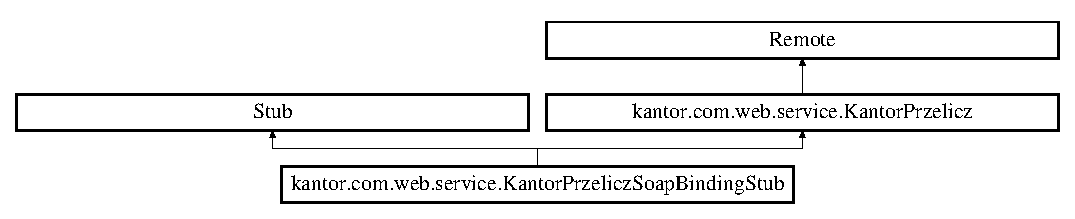
\includegraphics[height=2.492581cm]{classkantor_1_1com_1_1web_1_1service_1_1_kantor_przelicz_soap_binding_stub}
\end{center}
\end{figure}
\subsection*{Public Member Functions}
\begin{DoxyCompactItemize}
\item 
\hyperlink{classkantor_1_1com_1_1web_1_1service_1_1_kantor_przelicz_soap_binding_stub_a6c1f74a1f7117ce0ea705f95b1379c48}{Kantor\+Przelicz\+Soap\+Binding\+Stub} ()  throws org.\+apache.\+axis.\+Axis\+Fault 
\item 
\hyperlink{classkantor_1_1com_1_1web_1_1service_1_1_kantor_przelicz_soap_binding_stub_a184f971a2447a07891dc98a63c2e34f8}{Kantor\+Przelicz\+Soap\+Binding\+Stub} (java.\+net.\+U\+R\+L endpoint\+U\+R\+L, javax.\+xml.\+rpc.\+Service service)  throws org.\+apache.\+axis.\+Axis\+Fault 
\item 
\hyperlink{classkantor_1_1com_1_1web_1_1service_1_1_kantor_przelicz_soap_binding_stub_a7bc4e56824226c3446401756be37657b}{Kantor\+Przelicz\+Soap\+Binding\+Stub} (javax.\+xml.\+rpc.\+Service service)  throws org.\+apache.\+axis.\+Axis\+Fault 
\item 
double\mbox{[}$\,$\mbox{]} \hyperlink{classkantor_1_1com_1_1web_1_1service_1_1_kantor_przelicz_soap_binding_stub_a3ebaba4acb670e918a73250d4111afcf}{pobierz\+\_\+kursy\+\_\+walut} ()  throws java.\+rmi.\+Remote\+Exception 
\item 
double \hyperlink{classkantor_1_1com_1_1web_1_1service_1_1_kantor_przelicz_soap_binding_stub_a1189d528b2a2bc30b1d0dbd4cb3de879}{G\+B\+Pna\+P\+L\+N} (double value)  throws java.\+rmi.\+Remote\+Exception 
\item 
double \hyperlink{classkantor_1_1com_1_1web_1_1service_1_1_kantor_przelicz_soap_binding_stub_a9ee2c58b4dc1c11c5b434d4dcc391f9d}{P\+L\+Nna\+R\+U\+B} (double value)  throws java.\+rmi.\+Remote\+Exception 
\item 
double \hyperlink{classkantor_1_1com_1_1web_1_1service_1_1_kantor_przelicz_soap_binding_stub_a1640d46443427ccc4ac2e9fc78fbfdbc}{J\+P\+Yna\+P\+L\+N} (double value)  throws java.\+rmi.\+Remote\+Exception 
\item 
double \hyperlink{classkantor_1_1com_1_1web_1_1service_1_1_kantor_przelicz_soap_binding_stub_ac8cc82abe2de05d4ed53e0c44faf0669}{P\+L\+Nna\+G\+B\+P} (double value)  throws java.\+rmi.\+Remote\+Exception 
\item 
double \hyperlink{classkantor_1_1com_1_1web_1_1service_1_1_kantor_przelicz_soap_binding_stub_a642b141aac243d540b987f5269297354}{P\+L\+Nna\+J\+P\+Y} (double value)  throws java.\+rmi.\+Remote\+Exception 
\item 
double \hyperlink{classkantor_1_1com_1_1web_1_1service_1_1_kantor_przelicz_soap_binding_stub_a808bb2077397435895bf2fd9bf38d6c7}{R\+U\+Bna\+P\+L\+N} (double value)  throws java.\+rmi.\+Remote\+Exception 
\item 
double \hyperlink{classkantor_1_1com_1_1web_1_1service_1_1_kantor_przelicz_soap_binding_stub_a16867679e15bceab605c16b1b20ff89d}{U\+S\+Dna\+P\+L\+N} (double value)  throws java.\+rmi.\+Remote\+Exception 
\item 
double \hyperlink{classkantor_1_1com_1_1web_1_1service_1_1_kantor_przelicz_soap_binding_stub_a62a18092ec91b3391244ff5e678186ec}{P\+L\+Nna\+U\+S\+D} (double value)  throws java.\+rmi.\+Remote\+Exception 
\item 
double \hyperlink{classkantor_1_1com_1_1web_1_1service_1_1_kantor_przelicz_soap_binding_stub_a1ca4bcdbf6b3301c515be2ddb81a7689}{E\+U\+Rna\+P\+L\+N} (double value)  throws java.\+rmi.\+Remote\+Exception 
\item 
double \hyperlink{classkantor_1_1com_1_1web_1_1service_1_1_kantor_przelicz_soap_binding_stub_a889d3a09409acf8888638c2dce6ea86f}{P\+L\+Nna\+E\+U\+R} (double value)  throws java.\+rmi.\+Remote\+Exception 
\item 
double \hyperlink{classkantor_1_1com_1_1web_1_1service_1_1_kantor_przelicz_soap_binding_stub_a998215c43de5fc4a9f9cb3300347761a}{P\+L\+Nna\+C\+H\+E} (double value)  throws java.\+rmi.\+Remote\+Exception 
\item 
double \hyperlink{classkantor_1_1com_1_1web_1_1service_1_1_kantor_przelicz_soap_binding_stub_a95c3905cd703617b5c0355134546befc}{C\+H\+Ena\+P\+L\+N} (double value)  throws java.\+rmi.\+Remote\+Exception 
\end{DoxyCompactItemize}
\subsection*{Protected Member Functions}
\begin{DoxyCompactItemize}
\item 
org.\+apache.\+axis.\+client.\+Call \hyperlink{classkantor_1_1com_1_1web_1_1service_1_1_kantor_przelicz_soap_binding_stub_a48bdf944c0e7affdc54748a99e024768}{create\+Call} ()  throws java.\+rmi.\+Remote\+Exception 
\end{DoxyCompactItemize}


\subsection{Detailed Description}


Definition at line 10 of file Kantor\+Przelicz\+Soap\+Binding\+Stub.\+java.



\subsection{Constructor \& Destructor Documentation}
\hypertarget{classkantor_1_1com_1_1web_1_1service_1_1_kantor_przelicz_soap_binding_stub_a6c1f74a1f7117ce0ea705f95b1379c48}{\index{kantor\+::com\+::web\+::service\+::\+Kantor\+Przelicz\+Soap\+Binding\+Stub@{kantor\+::com\+::web\+::service\+::\+Kantor\+Przelicz\+Soap\+Binding\+Stub}!Kantor\+Przelicz\+Soap\+Binding\+Stub@{Kantor\+Przelicz\+Soap\+Binding\+Stub}}
\index{Kantor\+Przelicz\+Soap\+Binding\+Stub@{Kantor\+Przelicz\+Soap\+Binding\+Stub}!kantor\+::com\+::web\+::service\+::\+Kantor\+Przelicz\+Soap\+Binding\+Stub@{kantor\+::com\+::web\+::service\+::\+Kantor\+Przelicz\+Soap\+Binding\+Stub}}
\subsubsection[{Kantor\+Przelicz\+Soap\+Binding\+Stub}]{\setlength{\rightskip}{0pt plus 5cm}kantor.\+com.\+web.\+service.\+Kantor\+Przelicz\+Soap\+Binding\+Stub.\+Kantor\+Przelicz\+Soap\+Binding\+Stub (
\begin{DoxyParamCaption}
{}
\end{DoxyParamCaption}
) throws org.\+apache.\+axis.\+Axis\+Fault}}\label{classkantor_1_1com_1_1web_1_1service_1_1_kantor_przelicz_soap_binding_stub_a6c1f74a1f7117ce0ea705f95b1379c48}


Definition at line 175 of file Kantor\+Przelicz\+Soap\+Binding\+Stub.\+java.

\hypertarget{classkantor_1_1com_1_1web_1_1service_1_1_kantor_przelicz_soap_binding_stub_a184f971a2447a07891dc98a63c2e34f8}{\index{kantor\+::com\+::web\+::service\+::\+Kantor\+Przelicz\+Soap\+Binding\+Stub@{kantor\+::com\+::web\+::service\+::\+Kantor\+Przelicz\+Soap\+Binding\+Stub}!Kantor\+Przelicz\+Soap\+Binding\+Stub@{Kantor\+Przelicz\+Soap\+Binding\+Stub}}
\index{Kantor\+Przelicz\+Soap\+Binding\+Stub@{Kantor\+Przelicz\+Soap\+Binding\+Stub}!kantor\+::com\+::web\+::service\+::\+Kantor\+Przelicz\+Soap\+Binding\+Stub@{kantor\+::com\+::web\+::service\+::\+Kantor\+Przelicz\+Soap\+Binding\+Stub}}
\subsubsection[{Kantor\+Przelicz\+Soap\+Binding\+Stub}]{\setlength{\rightskip}{0pt plus 5cm}kantor.\+com.\+web.\+service.\+Kantor\+Przelicz\+Soap\+Binding\+Stub.\+Kantor\+Przelicz\+Soap\+Binding\+Stub (
\begin{DoxyParamCaption}
\item[{java.\+net.\+U\+R\+L}]{endpoint\+U\+R\+L, }
\item[{javax.\+xml.\+rpc.\+Service}]{service}
\end{DoxyParamCaption}
) throws org.\+apache.\+axis.\+Axis\+Fault}}\label{classkantor_1_1com_1_1web_1_1service_1_1_kantor_przelicz_soap_binding_stub_a184f971a2447a07891dc98a63c2e34f8}


Definition at line 179 of file Kantor\+Przelicz\+Soap\+Binding\+Stub.\+java.

\hypertarget{classkantor_1_1com_1_1web_1_1service_1_1_kantor_przelicz_soap_binding_stub_a7bc4e56824226c3446401756be37657b}{\index{kantor\+::com\+::web\+::service\+::\+Kantor\+Przelicz\+Soap\+Binding\+Stub@{kantor\+::com\+::web\+::service\+::\+Kantor\+Przelicz\+Soap\+Binding\+Stub}!Kantor\+Przelicz\+Soap\+Binding\+Stub@{Kantor\+Przelicz\+Soap\+Binding\+Stub}}
\index{Kantor\+Przelicz\+Soap\+Binding\+Stub@{Kantor\+Przelicz\+Soap\+Binding\+Stub}!kantor\+::com\+::web\+::service\+::\+Kantor\+Przelicz\+Soap\+Binding\+Stub@{kantor\+::com\+::web\+::service\+::\+Kantor\+Przelicz\+Soap\+Binding\+Stub}}
\subsubsection[{Kantor\+Przelicz\+Soap\+Binding\+Stub}]{\setlength{\rightskip}{0pt plus 5cm}kantor.\+com.\+web.\+service.\+Kantor\+Przelicz\+Soap\+Binding\+Stub.\+Kantor\+Przelicz\+Soap\+Binding\+Stub (
\begin{DoxyParamCaption}
\item[{javax.\+xml.\+rpc.\+Service}]{service}
\end{DoxyParamCaption}
) throws org.\+apache.\+axis.\+Axis\+Fault}}\label{classkantor_1_1com_1_1web_1_1service_1_1_kantor_przelicz_soap_binding_stub_a7bc4e56824226c3446401756be37657b}


Definition at line 184 of file Kantor\+Przelicz\+Soap\+Binding\+Stub.\+java.



\subsection{Member Function Documentation}
\hypertarget{classkantor_1_1com_1_1web_1_1service_1_1_kantor_przelicz_soap_binding_stub_a95c3905cd703617b5c0355134546befc}{\index{kantor\+::com\+::web\+::service\+::\+Kantor\+Przelicz\+Soap\+Binding\+Stub@{kantor\+::com\+::web\+::service\+::\+Kantor\+Przelicz\+Soap\+Binding\+Stub}!C\+H\+Ena\+P\+L\+N@{C\+H\+Ena\+P\+L\+N}}
\index{C\+H\+Ena\+P\+L\+N@{C\+H\+Ena\+P\+L\+N}!kantor\+::com\+::web\+::service\+::\+Kantor\+Przelicz\+Soap\+Binding\+Stub@{kantor\+::com\+::web\+::service\+::\+Kantor\+Przelicz\+Soap\+Binding\+Stub}}
\subsubsection[{C\+H\+Ena\+P\+L\+N}]{\setlength{\rightskip}{0pt plus 5cm}double kantor.\+com.\+web.\+service.\+Kantor\+Przelicz\+Soap\+Binding\+Stub.\+C\+H\+Ena\+P\+L\+N (
\begin{DoxyParamCaption}
\item[{double}]{value}
\end{DoxyParamCaption}
) throws java.\+rmi.\+Remote\+Exception}}\label{classkantor_1_1com_1_1web_1_1service_1_1_kantor_przelicz_soap_binding_stub_a95c3905cd703617b5c0355134546befc}


Implements \hyperlink{classkantor_1_1com_1_1web_1_1service_1_1_kantor_przelicz_acff8492d50d84cf718bca4c8b499d36a}{kantor.\+com.\+web.\+service.\+Kantor\+Przelicz}.



Definition at line 634 of file Kantor\+Przelicz\+Soap\+Binding\+Stub.\+java.

\hypertarget{classkantor_1_1com_1_1web_1_1service_1_1_kantor_przelicz_soap_binding_stub_a48bdf944c0e7affdc54748a99e024768}{\index{kantor\+::com\+::web\+::service\+::\+Kantor\+Przelicz\+Soap\+Binding\+Stub@{kantor\+::com\+::web\+::service\+::\+Kantor\+Przelicz\+Soap\+Binding\+Stub}!create\+Call@{create\+Call}}
\index{create\+Call@{create\+Call}!kantor\+::com\+::web\+::service\+::\+Kantor\+Przelicz\+Soap\+Binding\+Stub@{kantor\+::com\+::web\+::service\+::\+Kantor\+Przelicz\+Soap\+Binding\+Stub}}
\subsubsection[{create\+Call}]{\setlength{\rightskip}{0pt plus 5cm}org.\+apache.\+axis.\+client.\+Call kantor.\+com.\+web.\+service.\+Kantor\+Przelicz\+Soap\+Binding\+Stub.\+create\+Call (
\begin{DoxyParamCaption}
{}
\end{DoxyParamCaption}
) throws java.\+rmi.\+Remote\+Exception\hspace{0.3cm}{\ttfamily [protected]}}}\label{classkantor_1_1com_1_1web_1_1service_1_1_kantor_przelicz_soap_binding_stub_a48bdf944c0e7affdc54748a99e024768}


Definition at line 193 of file Kantor\+Przelicz\+Soap\+Binding\+Stub.\+java.

\hypertarget{classkantor_1_1com_1_1web_1_1service_1_1_kantor_przelicz_soap_binding_stub_a1ca4bcdbf6b3301c515be2ddb81a7689}{\index{kantor\+::com\+::web\+::service\+::\+Kantor\+Przelicz\+Soap\+Binding\+Stub@{kantor\+::com\+::web\+::service\+::\+Kantor\+Przelicz\+Soap\+Binding\+Stub}!E\+U\+Rna\+P\+L\+N@{E\+U\+Rna\+P\+L\+N}}
\index{E\+U\+Rna\+P\+L\+N@{E\+U\+Rna\+P\+L\+N}!kantor\+::com\+::web\+::service\+::\+Kantor\+Przelicz\+Soap\+Binding\+Stub@{kantor\+::com\+::web\+::service\+::\+Kantor\+Przelicz\+Soap\+Binding\+Stub}}
\subsubsection[{E\+U\+Rna\+P\+L\+N}]{\setlength{\rightskip}{0pt plus 5cm}double kantor.\+com.\+web.\+service.\+Kantor\+Przelicz\+Soap\+Binding\+Stub.\+E\+U\+Rna\+P\+L\+N (
\begin{DoxyParamCaption}
\item[{double}]{value}
\end{DoxyParamCaption}
) throws java.\+rmi.\+Remote\+Exception}}\label{classkantor_1_1com_1_1web_1_1service_1_1_kantor_przelicz_soap_binding_stub_a1ca4bcdbf6b3301c515be2ddb81a7689}


Implements \hyperlink{classkantor_1_1com_1_1web_1_1service_1_1_kantor_przelicz_af204b150c62165c836a1a0afd10c16b7}{kantor.\+com.\+web.\+service.\+Kantor\+Przelicz}.



Definition at line 532 of file Kantor\+Przelicz\+Soap\+Binding\+Stub.\+java.

\hypertarget{classkantor_1_1com_1_1web_1_1service_1_1_kantor_przelicz_soap_binding_stub_a1189d528b2a2bc30b1d0dbd4cb3de879}{\index{kantor\+::com\+::web\+::service\+::\+Kantor\+Przelicz\+Soap\+Binding\+Stub@{kantor\+::com\+::web\+::service\+::\+Kantor\+Przelicz\+Soap\+Binding\+Stub}!G\+B\+Pna\+P\+L\+N@{G\+B\+Pna\+P\+L\+N}}
\index{G\+B\+Pna\+P\+L\+N@{G\+B\+Pna\+P\+L\+N}!kantor\+::com\+::web\+::service\+::\+Kantor\+Przelicz\+Soap\+Binding\+Stub@{kantor\+::com\+::web\+::service\+::\+Kantor\+Przelicz\+Soap\+Binding\+Stub}}
\subsubsection[{G\+B\+Pna\+P\+L\+N}]{\setlength{\rightskip}{0pt plus 5cm}double kantor.\+com.\+web.\+service.\+Kantor\+Przelicz\+Soap\+Binding\+Stub.\+G\+B\+Pna\+P\+L\+N (
\begin{DoxyParamCaption}
\item[{double}]{value}
\end{DoxyParamCaption}
) throws java.\+rmi.\+Remote\+Exception}}\label{classkantor_1_1com_1_1web_1_1service_1_1_kantor_przelicz_soap_binding_stub_a1189d528b2a2bc30b1d0dbd4cb3de879}


Implements \hyperlink{classkantor_1_1com_1_1web_1_1service_1_1_kantor_przelicz_a64b58db5e686a08b4b1af648eb781a1c}{kantor.\+com.\+web.\+service.\+Kantor\+Przelicz}.



Definition at line 260 of file Kantor\+Przelicz\+Soap\+Binding\+Stub.\+java.

\hypertarget{classkantor_1_1com_1_1web_1_1service_1_1_kantor_przelicz_soap_binding_stub_a1640d46443427ccc4ac2e9fc78fbfdbc}{\index{kantor\+::com\+::web\+::service\+::\+Kantor\+Przelicz\+Soap\+Binding\+Stub@{kantor\+::com\+::web\+::service\+::\+Kantor\+Przelicz\+Soap\+Binding\+Stub}!J\+P\+Yna\+P\+L\+N@{J\+P\+Yna\+P\+L\+N}}
\index{J\+P\+Yna\+P\+L\+N@{J\+P\+Yna\+P\+L\+N}!kantor\+::com\+::web\+::service\+::\+Kantor\+Przelicz\+Soap\+Binding\+Stub@{kantor\+::com\+::web\+::service\+::\+Kantor\+Przelicz\+Soap\+Binding\+Stub}}
\subsubsection[{J\+P\+Yna\+P\+L\+N}]{\setlength{\rightskip}{0pt plus 5cm}double kantor.\+com.\+web.\+service.\+Kantor\+Przelicz\+Soap\+Binding\+Stub.\+J\+P\+Yna\+P\+L\+N (
\begin{DoxyParamCaption}
\item[{double}]{value}
\end{DoxyParamCaption}
) throws java.\+rmi.\+Remote\+Exception}}\label{classkantor_1_1com_1_1web_1_1service_1_1_kantor_przelicz_soap_binding_stub_a1640d46443427ccc4ac2e9fc78fbfdbc}


Implements \hyperlink{classkantor_1_1com_1_1web_1_1service_1_1_kantor_przelicz_a9e6f2e71874e1dd7b520d2da4427bae8}{kantor.\+com.\+web.\+service.\+Kantor\+Przelicz}.



Definition at line 328 of file Kantor\+Przelicz\+Soap\+Binding\+Stub.\+java.

\hypertarget{classkantor_1_1com_1_1web_1_1service_1_1_kantor_przelicz_soap_binding_stub_a998215c43de5fc4a9f9cb3300347761a}{\index{kantor\+::com\+::web\+::service\+::\+Kantor\+Przelicz\+Soap\+Binding\+Stub@{kantor\+::com\+::web\+::service\+::\+Kantor\+Przelicz\+Soap\+Binding\+Stub}!P\+L\+Nna\+C\+H\+E@{P\+L\+Nna\+C\+H\+E}}
\index{P\+L\+Nna\+C\+H\+E@{P\+L\+Nna\+C\+H\+E}!kantor\+::com\+::web\+::service\+::\+Kantor\+Przelicz\+Soap\+Binding\+Stub@{kantor\+::com\+::web\+::service\+::\+Kantor\+Przelicz\+Soap\+Binding\+Stub}}
\subsubsection[{P\+L\+Nna\+C\+H\+E}]{\setlength{\rightskip}{0pt plus 5cm}double kantor.\+com.\+web.\+service.\+Kantor\+Przelicz\+Soap\+Binding\+Stub.\+P\+L\+Nna\+C\+H\+E (
\begin{DoxyParamCaption}
\item[{double}]{value}
\end{DoxyParamCaption}
) throws java.\+rmi.\+Remote\+Exception}}\label{classkantor_1_1com_1_1web_1_1service_1_1_kantor_przelicz_soap_binding_stub_a998215c43de5fc4a9f9cb3300347761a}


Implements \hyperlink{classkantor_1_1com_1_1web_1_1service_1_1_kantor_przelicz_afa953802446690d409e1df5361729fc0}{kantor.\+com.\+web.\+service.\+Kantor\+Przelicz}.



Definition at line 600 of file Kantor\+Przelicz\+Soap\+Binding\+Stub.\+java.

\hypertarget{classkantor_1_1com_1_1web_1_1service_1_1_kantor_przelicz_soap_binding_stub_a889d3a09409acf8888638c2dce6ea86f}{\index{kantor\+::com\+::web\+::service\+::\+Kantor\+Przelicz\+Soap\+Binding\+Stub@{kantor\+::com\+::web\+::service\+::\+Kantor\+Przelicz\+Soap\+Binding\+Stub}!P\+L\+Nna\+E\+U\+R@{P\+L\+Nna\+E\+U\+R}}
\index{P\+L\+Nna\+E\+U\+R@{P\+L\+Nna\+E\+U\+R}!kantor\+::com\+::web\+::service\+::\+Kantor\+Przelicz\+Soap\+Binding\+Stub@{kantor\+::com\+::web\+::service\+::\+Kantor\+Przelicz\+Soap\+Binding\+Stub}}
\subsubsection[{P\+L\+Nna\+E\+U\+R}]{\setlength{\rightskip}{0pt plus 5cm}double kantor.\+com.\+web.\+service.\+Kantor\+Przelicz\+Soap\+Binding\+Stub.\+P\+L\+Nna\+E\+U\+R (
\begin{DoxyParamCaption}
\item[{double}]{value}
\end{DoxyParamCaption}
) throws java.\+rmi.\+Remote\+Exception}}\label{classkantor_1_1com_1_1web_1_1service_1_1_kantor_przelicz_soap_binding_stub_a889d3a09409acf8888638c2dce6ea86f}


Implements \hyperlink{classkantor_1_1com_1_1web_1_1service_1_1_kantor_przelicz_acfc0cd42fb64c5f26d468245cf0fe3b6}{kantor.\+com.\+web.\+service.\+Kantor\+Przelicz}.



Definition at line 566 of file Kantor\+Przelicz\+Soap\+Binding\+Stub.\+java.

\hypertarget{classkantor_1_1com_1_1web_1_1service_1_1_kantor_przelicz_soap_binding_stub_ac8cc82abe2de05d4ed53e0c44faf0669}{\index{kantor\+::com\+::web\+::service\+::\+Kantor\+Przelicz\+Soap\+Binding\+Stub@{kantor\+::com\+::web\+::service\+::\+Kantor\+Przelicz\+Soap\+Binding\+Stub}!P\+L\+Nna\+G\+B\+P@{P\+L\+Nna\+G\+B\+P}}
\index{P\+L\+Nna\+G\+B\+P@{P\+L\+Nna\+G\+B\+P}!kantor\+::com\+::web\+::service\+::\+Kantor\+Przelicz\+Soap\+Binding\+Stub@{kantor\+::com\+::web\+::service\+::\+Kantor\+Przelicz\+Soap\+Binding\+Stub}}
\subsubsection[{P\+L\+Nna\+G\+B\+P}]{\setlength{\rightskip}{0pt plus 5cm}double kantor.\+com.\+web.\+service.\+Kantor\+Przelicz\+Soap\+Binding\+Stub.\+P\+L\+Nna\+G\+B\+P (
\begin{DoxyParamCaption}
\item[{double}]{value}
\end{DoxyParamCaption}
) throws java.\+rmi.\+Remote\+Exception}}\label{classkantor_1_1com_1_1web_1_1service_1_1_kantor_przelicz_soap_binding_stub_ac8cc82abe2de05d4ed53e0c44faf0669}


Implements \hyperlink{classkantor_1_1com_1_1web_1_1service_1_1_kantor_przelicz_ad0840077798f333f948772590d1a402a}{kantor.\+com.\+web.\+service.\+Kantor\+Przelicz}.



Definition at line 362 of file Kantor\+Przelicz\+Soap\+Binding\+Stub.\+java.

\hypertarget{classkantor_1_1com_1_1web_1_1service_1_1_kantor_przelicz_soap_binding_stub_a642b141aac243d540b987f5269297354}{\index{kantor\+::com\+::web\+::service\+::\+Kantor\+Przelicz\+Soap\+Binding\+Stub@{kantor\+::com\+::web\+::service\+::\+Kantor\+Przelicz\+Soap\+Binding\+Stub}!P\+L\+Nna\+J\+P\+Y@{P\+L\+Nna\+J\+P\+Y}}
\index{P\+L\+Nna\+J\+P\+Y@{P\+L\+Nna\+J\+P\+Y}!kantor\+::com\+::web\+::service\+::\+Kantor\+Przelicz\+Soap\+Binding\+Stub@{kantor\+::com\+::web\+::service\+::\+Kantor\+Przelicz\+Soap\+Binding\+Stub}}
\subsubsection[{P\+L\+Nna\+J\+P\+Y}]{\setlength{\rightskip}{0pt plus 5cm}double kantor.\+com.\+web.\+service.\+Kantor\+Przelicz\+Soap\+Binding\+Stub.\+P\+L\+Nna\+J\+P\+Y (
\begin{DoxyParamCaption}
\item[{double}]{value}
\end{DoxyParamCaption}
) throws java.\+rmi.\+Remote\+Exception}}\label{classkantor_1_1com_1_1web_1_1service_1_1_kantor_przelicz_soap_binding_stub_a642b141aac243d540b987f5269297354}


Implements \hyperlink{classkantor_1_1com_1_1web_1_1service_1_1_kantor_przelicz_a7706e3a08c1b8ce3775506c4530d1bf7}{kantor.\+com.\+web.\+service.\+Kantor\+Przelicz}.



Definition at line 396 of file Kantor\+Przelicz\+Soap\+Binding\+Stub.\+java.

\hypertarget{classkantor_1_1com_1_1web_1_1service_1_1_kantor_przelicz_soap_binding_stub_a9ee2c58b4dc1c11c5b434d4dcc391f9d}{\index{kantor\+::com\+::web\+::service\+::\+Kantor\+Przelicz\+Soap\+Binding\+Stub@{kantor\+::com\+::web\+::service\+::\+Kantor\+Przelicz\+Soap\+Binding\+Stub}!P\+L\+Nna\+R\+U\+B@{P\+L\+Nna\+R\+U\+B}}
\index{P\+L\+Nna\+R\+U\+B@{P\+L\+Nna\+R\+U\+B}!kantor\+::com\+::web\+::service\+::\+Kantor\+Przelicz\+Soap\+Binding\+Stub@{kantor\+::com\+::web\+::service\+::\+Kantor\+Przelicz\+Soap\+Binding\+Stub}}
\subsubsection[{P\+L\+Nna\+R\+U\+B}]{\setlength{\rightskip}{0pt plus 5cm}double kantor.\+com.\+web.\+service.\+Kantor\+Przelicz\+Soap\+Binding\+Stub.\+P\+L\+Nna\+R\+U\+B (
\begin{DoxyParamCaption}
\item[{double}]{value}
\end{DoxyParamCaption}
) throws java.\+rmi.\+Remote\+Exception}}\label{classkantor_1_1com_1_1web_1_1service_1_1_kantor_przelicz_soap_binding_stub_a9ee2c58b4dc1c11c5b434d4dcc391f9d}


Implements \hyperlink{classkantor_1_1com_1_1web_1_1service_1_1_kantor_przelicz_ad68cbeb18f18cd02c3b4b571da0e06fa}{kantor.\+com.\+web.\+service.\+Kantor\+Przelicz}.



Definition at line 294 of file Kantor\+Przelicz\+Soap\+Binding\+Stub.\+java.

\hypertarget{classkantor_1_1com_1_1web_1_1service_1_1_kantor_przelicz_soap_binding_stub_a62a18092ec91b3391244ff5e678186ec}{\index{kantor\+::com\+::web\+::service\+::\+Kantor\+Przelicz\+Soap\+Binding\+Stub@{kantor\+::com\+::web\+::service\+::\+Kantor\+Przelicz\+Soap\+Binding\+Stub}!P\+L\+Nna\+U\+S\+D@{P\+L\+Nna\+U\+S\+D}}
\index{P\+L\+Nna\+U\+S\+D@{P\+L\+Nna\+U\+S\+D}!kantor\+::com\+::web\+::service\+::\+Kantor\+Przelicz\+Soap\+Binding\+Stub@{kantor\+::com\+::web\+::service\+::\+Kantor\+Przelicz\+Soap\+Binding\+Stub}}
\subsubsection[{P\+L\+Nna\+U\+S\+D}]{\setlength{\rightskip}{0pt plus 5cm}double kantor.\+com.\+web.\+service.\+Kantor\+Przelicz\+Soap\+Binding\+Stub.\+P\+L\+Nna\+U\+S\+D (
\begin{DoxyParamCaption}
\item[{double}]{value}
\end{DoxyParamCaption}
) throws java.\+rmi.\+Remote\+Exception}}\label{classkantor_1_1com_1_1web_1_1service_1_1_kantor_przelicz_soap_binding_stub_a62a18092ec91b3391244ff5e678186ec}


Implements \hyperlink{classkantor_1_1com_1_1web_1_1service_1_1_kantor_przelicz_aea3a5dd74cf10d0c9ce1bf04b94078c8}{kantor.\+com.\+web.\+service.\+Kantor\+Przelicz}.



Definition at line 498 of file Kantor\+Przelicz\+Soap\+Binding\+Stub.\+java.

\hypertarget{classkantor_1_1com_1_1web_1_1service_1_1_kantor_przelicz_soap_binding_stub_a3ebaba4acb670e918a73250d4111afcf}{\index{kantor\+::com\+::web\+::service\+::\+Kantor\+Przelicz\+Soap\+Binding\+Stub@{kantor\+::com\+::web\+::service\+::\+Kantor\+Przelicz\+Soap\+Binding\+Stub}!pobierz\+\_\+kursy\+\_\+walut@{pobierz\+\_\+kursy\+\_\+walut}}
\index{pobierz\+\_\+kursy\+\_\+walut@{pobierz\+\_\+kursy\+\_\+walut}!kantor\+::com\+::web\+::service\+::\+Kantor\+Przelicz\+Soap\+Binding\+Stub@{kantor\+::com\+::web\+::service\+::\+Kantor\+Przelicz\+Soap\+Binding\+Stub}}
\subsubsection[{pobierz\+\_\+kursy\+\_\+walut}]{\setlength{\rightskip}{0pt plus 5cm}double \mbox{[}$\,$\mbox{]} kantor.\+com.\+web.\+service.\+Kantor\+Przelicz\+Soap\+Binding\+Stub.\+pobierz\+\_\+kursy\+\_\+walut (
\begin{DoxyParamCaption}
{}
\end{DoxyParamCaption}
) throws java.\+rmi.\+Remote\+Exception}}\label{classkantor_1_1com_1_1web_1_1service_1_1_kantor_przelicz_soap_binding_stub_a3ebaba4acb670e918a73250d4111afcf}


Implements \hyperlink{classkantor_1_1com_1_1web_1_1service_1_1_kantor_przelicz_a9e2610a2cdb76ea7e2551786f3c0736e}{kantor.\+com.\+web.\+service.\+Kantor\+Przelicz}.



Definition at line 226 of file Kantor\+Przelicz\+Soap\+Binding\+Stub.\+java.

\hypertarget{classkantor_1_1com_1_1web_1_1service_1_1_kantor_przelicz_soap_binding_stub_a808bb2077397435895bf2fd9bf38d6c7}{\index{kantor\+::com\+::web\+::service\+::\+Kantor\+Przelicz\+Soap\+Binding\+Stub@{kantor\+::com\+::web\+::service\+::\+Kantor\+Przelicz\+Soap\+Binding\+Stub}!R\+U\+Bna\+P\+L\+N@{R\+U\+Bna\+P\+L\+N}}
\index{R\+U\+Bna\+P\+L\+N@{R\+U\+Bna\+P\+L\+N}!kantor\+::com\+::web\+::service\+::\+Kantor\+Przelicz\+Soap\+Binding\+Stub@{kantor\+::com\+::web\+::service\+::\+Kantor\+Przelicz\+Soap\+Binding\+Stub}}
\subsubsection[{R\+U\+Bna\+P\+L\+N}]{\setlength{\rightskip}{0pt plus 5cm}double kantor.\+com.\+web.\+service.\+Kantor\+Przelicz\+Soap\+Binding\+Stub.\+R\+U\+Bna\+P\+L\+N (
\begin{DoxyParamCaption}
\item[{double}]{value}
\end{DoxyParamCaption}
) throws java.\+rmi.\+Remote\+Exception}}\label{classkantor_1_1com_1_1web_1_1service_1_1_kantor_przelicz_soap_binding_stub_a808bb2077397435895bf2fd9bf38d6c7}


Implements \hyperlink{classkantor_1_1com_1_1web_1_1service_1_1_kantor_przelicz_a11c3958baf84a3a96dbc9290890b6c4e}{kantor.\+com.\+web.\+service.\+Kantor\+Przelicz}.



Definition at line 430 of file Kantor\+Przelicz\+Soap\+Binding\+Stub.\+java.

\hypertarget{classkantor_1_1com_1_1web_1_1service_1_1_kantor_przelicz_soap_binding_stub_a16867679e15bceab605c16b1b20ff89d}{\index{kantor\+::com\+::web\+::service\+::\+Kantor\+Przelicz\+Soap\+Binding\+Stub@{kantor\+::com\+::web\+::service\+::\+Kantor\+Przelicz\+Soap\+Binding\+Stub}!U\+S\+Dna\+P\+L\+N@{U\+S\+Dna\+P\+L\+N}}
\index{U\+S\+Dna\+P\+L\+N@{U\+S\+Dna\+P\+L\+N}!kantor\+::com\+::web\+::service\+::\+Kantor\+Przelicz\+Soap\+Binding\+Stub@{kantor\+::com\+::web\+::service\+::\+Kantor\+Przelicz\+Soap\+Binding\+Stub}}
\subsubsection[{U\+S\+Dna\+P\+L\+N}]{\setlength{\rightskip}{0pt plus 5cm}double kantor.\+com.\+web.\+service.\+Kantor\+Przelicz\+Soap\+Binding\+Stub.\+U\+S\+Dna\+P\+L\+N (
\begin{DoxyParamCaption}
\item[{double}]{value}
\end{DoxyParamCaption}
) throws java.\+rmi.\+Remote\+Exception}}\label{classkantor_1_1com_1_1web_1_1service_1_1_kantor_przelicz_soap_binding_stub_a16867679e15bceab605c16b1b20ff89d}


Implements \hyperlink{classkantor_1_1com_1_1web_1_1service_1_1_kantor_przelicz_ad263683559db773d4ccb28e14090824f}{kantor.\+com.\+web.\+service.\+Kantor\+Przelicz}.



Definition at line 464 of file Kantor\+Przelicz\+Soap\+Binding\+Stub.\+java.



The documentation for this class was generated from the following file\+:\begin{DoxyCompactItemize}
\item 
C\+:/\+Users/kuska/\+Desktop/\+Michalik/\+K\+W/\+Kantor\+W\+S\+Client/src/kantor/com/web/service/\hyperlink{_kantor_przelicz_soap_binding_stub_8java}{Kantor\+Przelicz\+Soap\+Binding\+Stub.\+java}\end{DoxyCompactItemize}

\hypertarget{classkantor_1_1com_1_1web_1_1service_1_1_kursy_pokaz}{\section{kantor.\+com.\+web.\+service.\+Kursy\+Pokaz Interface Reference}
\label{classkantor_1_1com_1_1web_1_1service_1_1_kursy_pokaz}\index{kantor.\+com.\+web.\+service.\+Kursy\+Pokaz@{kantor.\+com.\+web.\+service.\+Kursy\+Pokaz}}
}
Inheritance diagram for kantor.\+com.\+web.\+service.\+Kursy\+Pokaz\+:\begin{figure}[H]
\begin{center}
\leavevmode
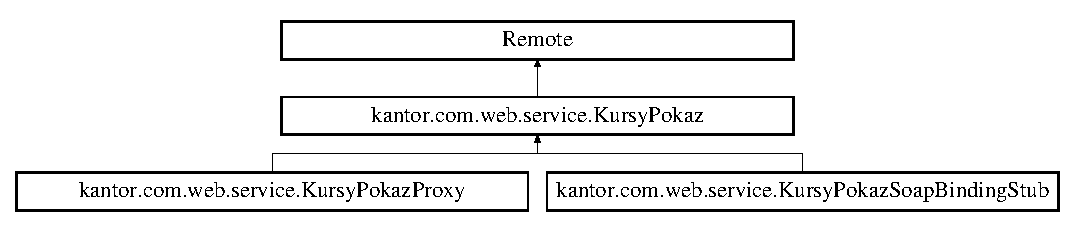
\includegraphics[height=2.608696cm]{classkantor_1_1com_1_1web_1_1service_1_1_kursy_pokaz}
\end{center}
\end{figure}
\subsection*{Public Member Functions}
\begin{DoxyCompactItemize}
\item 
double \hyperlink{classkantor_1_1com_1_1web_1_1service_1_1_kursy_pokaz_a31eef9def09b0841facda085644ede65}{E\+U\+Rna\+P\+L\+N} ()
\item 
double \hyperlink{classkantor_1_1com_1_1web_1_1service_1_1_kursy_pokaz_a26efb7c3127847ac0bd6adf865c4b891}{P\+L\+Nna\+U\+S\+D} ()
\item 
double \hyperlink{classkantor_1_1com_1_1web_1_1service_1_1_kursy_pokaz_a2c8884d959ed13948edc408b94083b95}{U\+S\+Dna\+P\+L\+N} ()
\item 
double \hyperlink{classkantor_1_1com_1_1web_1_1service_1_1_kursy_pokaz_a31eef9def09b0841facda085644ede65}{E\+U\+Rna\+P\+L\+N} ()  throws java.\+rmi.\+Remote\+Exception
\item 
double \hyperlink{classkantor_1_1com_1_1web_1_1service_1_1_kursy_pokaz_a758e416bdc0cdec7848747c2ceb5818e}{P\+L\+Nna\+E\+U\+R} ()  throws java.\+rmi.\+Remote\+Exception
\item 
double \hyperlink{classkantor_1_1com_1_1web_1_1service_1_1_kursy_pokaz_a26efb7c3127847ac0bd6adf865c4b891}{P\+L\+Nna\+U\+S\+D} ()  throws java.\+rmi.\+Remote\+Exception
\item 
double \hyperlink{classkantor_1_1com_1_1web_1_1service_1_1_kursy_pokaz_a2c8884d959ed13948edc408b94083b95}{U\+S\+Dna\+P\+L\+N} ()  throws java.\+rmi.\+Remote\+Exception
\end{DoxyCompactItemize}


\subsection{Detailed Description}


Definition at line 3 of file Kursy\+Pokaz.\+java.



\subsection{Member Function Documentation}
\hypertarget{classkantor_1_1com_1_1web_1_1service_1_1_kursy_pokaz_a31eef9def09b0841facda085644ede65}{\index{kantor\+::com\+::web\+::service\+::\+Kursy\+Pokaz@{kantor\+::com\+::web\+::service\+::\+Kursy\+Pokaz}!E\+U\+Rna\+P\+L\+N@{E\+U\+Rna\+P\+L\+N}}
\index{E\+U\+Rna\+P\+L\+N@{E\+U\+Rna\+P\+L\+N}!kantor\+::com\+::web\+::service\+::\+Kursy\+Pokaz@{kantor\+::com\+::web\+::service\+::\+Kursy\+Pokaz}}
\subsubsection[{E\+U\+Rna\+P\+L\+N}]{\setlength{\rightskip}{0pt plus 5cm}double kantor.\+com.\+web.\+service.\+Kursy\+Pokaz.\+E\+U\+Rna\+P\+L\+N (
\begin{DoxyParamCaption}
{}
\end{DoxyParamCaption}
)}}\label{classkantor_1_1com_1_1web_1_1service_1_1_kursy_pokaz_a31eef9def09b0841facda085644ede65}


Implemented in \hyperlink{classkantor_1_1com_1_1web_1_1service_1_1_kursy_pokaz_soap_binding_stub_a3e89646ddaed6b605071d1f6d186e66e}{kantor.\+com.\+web.\+service.\+Kursy\+Pokaz\+Soap\+Binding\+Stub}, and \hyperlink{classkantor_1_1com_1_1web_1_1service_1_1_kursy_pokaz_proxy_aa16bd4e29f240c450407162dea41a319}{kantor.\+com.\+web.\+service.\+Kursy\+Pokaz\+Proxy}.



Definition at line 4 of file Kursy\+Pokaz.\+java.

\hypertarget{classkantor_1_1com_1_1web_1_1service_1_1_kursy_pokaz_a31eef9def09b0841facda085644ede65}{\index{kantor\+::com\+::web\+::service\+::\+Kursy\+Pokaz@{kantor\+::com\+::web\+::service\+::\+Kursy\+Pokaz}!E\+U\+Rna\+P\+L\+N@{E\+U\+Rna\+P\+L\+N}}
\index{E\+U\+Rna\+P\+L\+N@{E\+U\+Rna\+P\+L\+N}!kantor\+::com\+::web\+::service\+::\+Kursy\+Pokaz@{kantor\+::com\+::web\+::service\+::\+Kursy\+Pokaz}}
\subsubsection[{E\+U\+Rna\+P\+L\+N}]{\setlength{\rightskip}{0pt plus 5cm}double kantor.\+com.\+web.\+service.\+Kursy\+Pokaz.\+E\+U\+Rna\+P\+L\+N (
\begin{DoxyParamCaption}
{}
\end{DoxyParamCaption}
) throws java.\+rmi.\+Remote\+Exception}}\label{classkantor_1_1com_1_1web_1_1service_1_1_kursy_pokaz_a31eef9def09b0841facda085644ede65}


Implemented in \hyperlink{classkantor_1_1com_1_1web_1_1service_1_1_kursy_pokaz_soap_binding_stub_a3e89646ddaed6b605071d1f6d186e66e}{kantor.\+com.\+web.\+service.\+Kursy\+Pokaz\+Soap\+Binding\+Stub}, and \hyperlink{classkantor_1_1com_1_1web_1_1service_1_1_kursy_pokaz_proxy_aa16bd4e29f240c450407162dea41a319}{kantor.\+com.\+web.\+service.\+Kursy\+Pokaz\+Proxy}.

\hypertarget{classkantor_1_1com_1_1web_1_1service_1_1_kursy_pokaz_a758e416bdc0cdec7848747c2ceb5818e}{\index{kantor\+::com\+::web\+::service\+::\+Kursy\+Pokaz@{kantor\+::com\+::web\+::service\+::\+Kursy\+Pokaz}!P\+L\+Nna\+E\+U\+R@{P\+L\+Nna\+E\+U\+R}}
\index{P\+L\+Nna\+E\+U\+R@{P\+L\+Nna\+E\+U\+R}!kantor\+::com\+::web\+::service\+::\+Kursy\+Pokaz@{kantor\+::com\+::web\+::service\+::\+Kursy\+Pokaz}}
\subsubsection[{P\+L\+Nna\+E\+U\+R}]{\setlength{\rightskip}{0pt plus 5cm}double kantor.\+com.\+web.\+service.\+Kursy\+Pokaz.\+P\+L\+Nna\+E\+U\+R (
\begin{DoxyParamCaption}
{}
\end{DoxyParamCaption}
) throws java.\+rmi.\+Remote\+Exception}}\label{classkantor_1_1com_1_1web_1_1service_1_1_kursy_pokaz_a758e416bdc0cdec7848747c2ceb5818e}


Implemented in \hyperlink{classkantor_1_1com_1_1web_1_1service_1_1_kursy_pokaz_soap_binding_stub_a6dd0efcbf660c065637f49570889f41d}{kantor.\+com.\+web.\+service.\+Kursy\+Pokaz\+Soap\+Binding\+Stub}, and \hyperlink{classkantor_1_1com_1_1web_1_1service_1_1_kursy_pokaz_proxy_ac1c39363de8b4da0827bf5f9f2014bed}{kantor.\+com.\+web.\+service.\+Kursy\+Pokaz\+Proxy}.

\hypertarget{classkantor_1_1com_1_1web_1_1service_1_1_kursy_pokaz_a26efb7c3127847ac0bd6adf865c4b891}{\index{kantor\+::com\+::web\+::service\+::\+Kursy\+Pokaz@{kantor\+::com\+::web\+::service\+::\+Kursy\+Pokaz}!P\+L\+Nna\+U\+S\+D@{P\+L\+Nna\+U\+S\+D}}
\index{P\+L\+Nna\+U\+S\+D@{P\+L\+Nna\+U\+S\+D}!kantor\+::com\+::web\+::service\+::\+Kursy\+Pokaz@{kantor\+::com\+::web\+::service\+::\+Kursy\+Pokaz}}
\subsubsection[{P\+L\+Nna\+U\+S\+D}]{\setlength{\rightskip}{0pt plus 5cm}double kantor.\+com.\+web.\+service.\+Kursy\+Pokaz.\+P\+L\+Nna\+U\+S\+D (
\begin{DoxyParamCaption}
{}
\end{DoxyParamCaption}
)}}\label{classkantor_1_1com_1_1web_1_1service_1_1_kursy_pokaz_a26efb7c3127847ac0bd6adf865c4b891}


Implemented in \hyperlink{classkantor_1_1com_1_1web_1_1service_1_1_kursy_pokaz_soap_binding_stub_a2f975ee29635758cd503316c16ba179c}{kantor.\+com.\+web.\+service.\+Kursy\+Pokaz\+Soap\+Binding\+Stub}, and \hyperlink{classkantor_1_1com_1_1web_1_1service_1_1_kursy_pokaz_proxy_a52629df59f3ebd199c6080496a755fda}{kantor.\+com.\+web.\+service.\+Kursy\+Pokaz\+Proxy}.



Definition at line 8 of file Kursy\+Pokaz.\+java.

\hypertarget{classkantor_1_1com_1_1web_1_1service_1_1_kursy_pokaz_a26efb7c3127847ac0bd6adf865c4b891}{\index{kantor\+::com\+::web\+::service\+::\+Kursy\+Pokaz@{kantor\+::com\+::web\+::service\+::\+Kursy\+Pokaz}!P\+L\+Nna\+U\+S\+D@{P\+L\+Nna\+U\+S\+D}}
\index{P\+L\+Nna\+U\+S\+D@{P\+L\+Nna\+U\+S\+D}!kantor\+::com\+::web\+::service\+::\+Kursy\+Pokaz@{kantor\+::com\+::web\+::service\+::\+Kursy\+Pokaz}}
\subsubsection[{P\+L\+Nna\+U\+S\+D}]{\setlength{\rightskip}{0pt plus 5cm}double kantor.\+com.\+web.\+service.\+Kursy\+Pokaz.\+P\+L\+Nna\+U\+S\+D (
\begin{DoxyParamCaption}
{}
\end{DoxyParamCaption}
) throws java.\+rmi.\+Remote\+Exception}}\label{classkantor_1_1com_1_1web_1_1service_1_1_kursy_pokaz_a26efb7c3127847ac0bd6adf865c4b891}


Implemented in \hyperlink{classkantor_1_1com_1_1web_1_1service_1_1_kursy_pokaz_soap_binding_stub_a2f975ee29635758cd503316c16ba179c}{kantor.\+com.\+web.\+service.\+Kursy\+Pokaz\+Soap\+Binding\+Stub}, and \hyperlink{classkantor_1_1com_1_1web_1_1service_1_1_kursy_pokaz_proxy_a52629df59f3ebd199c6080496a755fda}{kantor.\+com.\+web.\+service.\+Kursy\+Pokaz\+Proxy}.

\hypertarget{classkantor_1_1com_1_1web_1_1service_1_1_kursy_pokaz_a2c8884d959ed13948edc408b94083b95}{\index{kantor\+::com\+::web\+::service\+::\+Kursy\+Pokaz@{kantor\+::com\+::web\+::service\+::\+Kursy\+Pokaz}!U\+S\+Dna\+P\+L\+N@{U\+S\+Dna\+P\+L\+N}}
\index{U\+S\+Dna\+P\+L\+N@{U\+S\+Dna\+P\+L\+N}!kantor\+::com\+::web\+::service\+::\+Kursy\+Pokaz@{kantor\+::com\+::web\+::service\+::\+Kursy\+Pokaz}}
\subsubsection[{U\+S\+Dna\+P\+L\+N}]{\setlength{\rightskip}{0pt plus 5cm}double kantor.\+com.\+web.\+service.\+Kursy\+Pokaz.\+U\+S\+Dna\+P\+L\+N (
\begin{DoxyParamCaption}
{}
\end{DoxyParamCaption}
)}}\label{classkantor_1_1com_1_1web_1_1service_1_1_kursy_pokaz_a2c8884d959ed13948edc408b94083b95}


Implemented in \hyperlink{classkantor_1_1com_1_1web_1_1service_1_1_kursy_pokaz_soap_binding_stub_aa8b296ac90b4ab4c880652527c013db2}{kantor.\+com.\+web.\+service.\+Kursy\+Pokaz\+Soap\+Binding\+Stub}, and \hyperlink{classkantor_1_1com_1_1web_1_1service_1_1_kursy_pokaz_proxy_a6a121fca243445158448a43bbd350403}{kantor.\+com.\+web.\+service.\+Kursy\+Pokaz\+Proxy}.



Definition at line 12 of file Kursy\+Pokaz.\+java.

\hypertarget{classkantor_1_1com_1_1web_1_1service_1_1_kursy_pokaz_a2c8884d959ed13948edc408b94083b95}{\index{kantor\+::com\+::web\+::service\+::\+Kursy\+Pokaz@{kantor\+::com\+::web\+::service\+::\+Kursy\+Pokaz}!U\+S\+Dna\+P\+L\+N@{U\+S\+Dna\+P\+L\+N}}
\index{U\+S\+Dna\+P\+L\+N@{U\+S\+Dna\+P\+L\+N}!kantor\+::com\+::web\+::service\+::\+Kursy\+Pokaz@{kantor\+::com\+::web\+::service\+::\+Kursy\+Pokaz}}
\subsubsection[{U\+S\+Dna\+P\+L\+N}]{\setlength{\rightskip}{0pt plus 5cm}double kantor.\+com.\+web.\+service.\+Kursy\+Pokaz.\+U\+S\+Dna\+P\+L\+N (
\begin{DoxyParamCaption}
{}
\end{DoxyParamCaption}
) throws java.\+rmi.\+Remote\+Exception}}\label{classkantor_1_1com_1_1web_1_1service_1_1_kursy_pokaz_a2c8884d959ed13948edc408b94083b95}


Implemented in \hyperlink{classkantor_1_1com_1_1web_1_1service_1_1_kursy_pokaz_soap_binding_stub_aa8b296ac90b4ab4c880652527c013db2}{kantor.\+com.\+web.\+service.\+Kursy\+Pokaz\+Soap\+Binding\+Stub}, and \hyperlink{classkantor_1_1com_1_1web_1_1service_1_1_kursy_pokaz_proxy_a6a121fca243445158448a43bbd350403}{kantor.\+com.\+web.\+service.\+Kursy\+Pokaz\+Proxy}.



The documentation for this interface was generated from the following file\+:\begin{DoxyCompactItemize}
\item 
C\+:/\+Users/kuska/\+Desktop/\+Michalik/\+K\+W/\+Kantor\+W\+S/src/kantor/com/web/service/\hyperlink{src_2kantor_2com_2web_2service_2_kursy_pokaz_8java}{Kursy\+Pokaz.\+java}\end{DoxyCompactItemize}

\hypertarget{classkantor_1_1com_1_1web_1_1service_1_1_kursy_pokaz_proxy}{\section{kantor.\+com.\+web.\+service.\+Kursy\+Pokaz\+Proxy Class Reference}
\label{classkantor_1_1com_1_1web_1_1service_1_1_kursy_pokaz_proxy}\index{kantor.\+com.\+web.\+service.\+Kursy\+Pokaz\+Proxy@{kantor.\+com.\+web.\+service.\+Kursy\+Pokaz\+Proxy}}
}
Inheritance diagram for kantor.\+com.\+web.\+service.\+Kursy\+Pokaz\+Proxy\+:\begin{figure}[H]
\begin{center}
\leavevmode
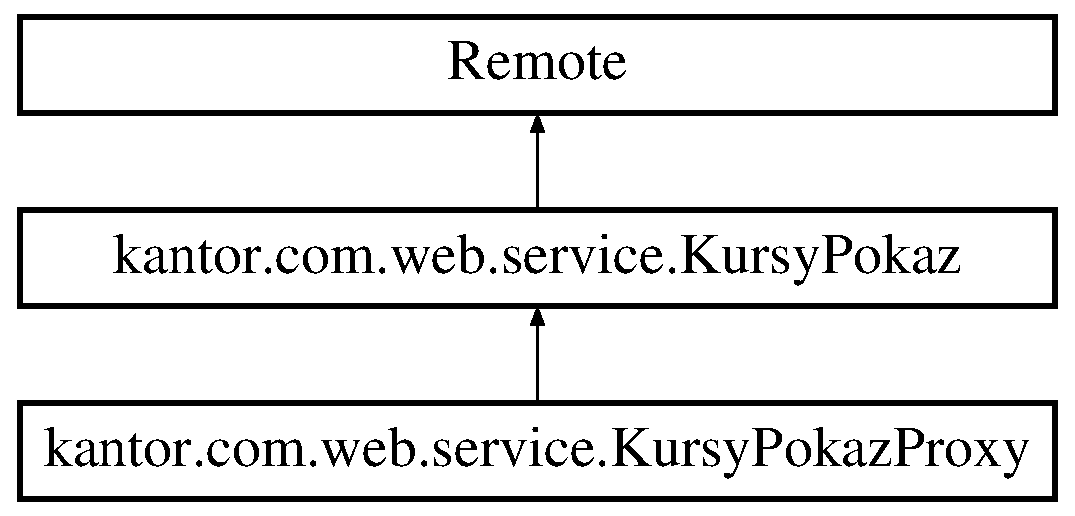
\includegraphics[height=3.000000cm]{classkantor_1_1com_1_1web_1_1service_1_1_kursy_pokaz_proxy}
\end{center}
\end{figure}
\subsection*{Public Member Functions}
\begin{DoxyCompactItemize}
\item 
\hyperlink{classkantor_1_1com_1_1web_1_1service_1_1_kursy_pokaz_proxy_ae6cdeaadabceecc54919a6f1bd95324c}{Kursy\+Pokaz\+Proxy} ()
\item 
\hyperlink{classkantor_1_1com_1_1web_1_1service_1_1_kursy_pokaz_proxy_ac9c9cc06f2cb753581fc755c190c87d2}{Kursy\+Pokaz\+Proxy} (String endpoint)
\item 
String \hyperlink{classkantor_1_1com_1_1web_1_1service_1_1_kursy_pokaz_proxy_a42ed01fce4a879671d1eaf934aa5f04f}{get\+Endpoint} ()
\item 
void \hyperlink{classkantor_1_1com_1_1web_1_1service_1_1_kursy_pokaz_proxy_a80ada94218bc9a193387e22b5a6dce0a}{set\+Endpoint} (String endpoint)
\item 
\hyperlink{classkantor_1_1com_1_1web_1_1service_1_1_kursy_pokaz}{kantor.\+com.\+web.\+service.\+Kursy\+Pokaz} \hyperlink{classkantor_1_1com_1_1web_1_1service_1_1_kursy_pokaz_proxy_a6d65d3963ffa4efb031cca95e183a296}{get\+Kursy\+Pokaz} ()
\item 
double \hyperlink{classkantor_1_1com_1_1web_1_1service_1_1_kursy_pokaz_proxy_aa16bd4e29f240c450407162dea41a319}{E\+U\+Rna\+P\+L\+N} ()  throws java.\+rmi.\+Remote\+Exception
\item 
double \hyperlink{classkantor_1_1com_1_1web_1_1service_1_1_kursy_pokaz_proxy_ac1c39363de8b4da0827bf5f9f2014bed}{P\+L\+Nna\+E\+U\+R} ()  throws java.\+rmi.\+Remote\+Exception
\item 
double \hyperlink{classkantor_1_1com_1_1web_1_1service_1_1_kursy_pokaz_proxy_a52629df59f3ebd199c6080496a755fda}{P\+L\+Nna\+U\+S\+D} ()  throws java.\+rmi.\+Remote\+Exception
\item 
double \hyperlink{classkantor_1_1com_1_1web_1_1service_1_1_kursy_pokaz_proxy_a6a121fca243445158448a43bbd350403}{U\+S\+Dna\+P\+L\+N} ()  throws java.\+rmi.\+Remote\+Exception
\end{DoxyCompactItemize}


\subsection{Detailed Description}


Definition at line 3 of file Kursy\+Pokaz\+Proxy.\+java.



\subsection{Constructor \& Destructor Documentation}
\hypertarget{classkantor_1_1com_1_1web_1_1service_1_1_kursy_pokaz_proxy_ae6cdeaadabceecc54919a6f1bd95324c}{\index{kantor\+::com\+::web\+::service\+::\+Kursy\+Pokaz\+Proxy@{kantor\+::com\+::web\+::service\+::\+Kursy\+Pokaz\+Proxy}!Kursy\+Pokaz\+Proxy@{Kursy\+Pokaz\+Proxy}}
\index{Kursy\+Pokaz\+Proxy@{Kursy\+Pokaz\+Proxy}!kantor\+::com\+::web\+::service\+::\+Kursy\+Pokaz\+Proxy@{kantor\+::com\+::web\+::service\+::\+Kursy\+Pokaz\+Proxy}}
\subsubsection[{Kursy\+Pokaz\+Proxy}]{\setlength{\rightskip}{0pt plus 5cm}kantor.\+com.\+web.\+service.\+Kursy\+Pokaz\+Proxy.\+Kursy\+Pokaz\+Proxy (
\begin{DoxyParamCaption}
{}
\end{DoxyParamCaption}
)}}\label{classkantor_1_1com_1_1web_1_1service_1_1_kursy_pokaz_proxy_ae6cdeaadabceecc54919a6f1bd95324c}


Definition at line 7 of file Kursy\+Pokaz\+Proxy.\+java.

\hypertarget{classkantor_1_1com_1_1web_1_1service_1_1_kursy_pokaz_proxy_ac9c9cc06f2cb753581fc755c190c87d2}{\index{kantor\+::com\+::web\+::service\+::\+Kursy\+Pokaz\+Proxy@{kantor\+::com\+::web\+::service\+::\+Kursy\+Pokaz\+Proxy}!Kursy\+Pokaz\+Proxy@{Kursy\+Pokaz\+Proxy}}
\index{Kursy\+Pokaz\+Proxy@{Kursy\+Pokaz\+Proxy}!kantor\+::com\+::web\+::service\+::\+Kursy\+Pokaz\+Proxy@{kantor\+::com\+::web\+::service\+::\+Kursy\+Pokaz\+Proxy}}
\subsubsection[{Kursy\+Pokaz\+Proxy}]{\setlength{\rightskip}{0pt plus 5cm}kantor.\+com.\+web.\+service.\+Kursy\+Pokaz\+Proxy.\+Kursy\+Pokaz\+Proxy (
\begin{DoxyParamCaption}
\item[{String}]{endpoint}
\end{DoxyParamCaption}
)}}\label{classkantor_1_1com_1_1web_1_1service_1_1_kursy_pokaz_proxy_ac9c9cc06f2cb753581fc755c190c87d2}


Definition at line 11 of file Kursy\+Pokaz\+Proxy.\+java.



\subsection{Member Function Documentation}
\hypertarget{classkantor_1_1com_1_1web_1_1service_1_1_kursy_pokaz_proxy_aa16bd4e29f240c450407162dea41a319}{\index{kantor\+::com\+::web\+::service\+::\+Kursy\+Pokaz\+Proxy@{kantor\+::com\+::web\+::service\+::\+Kursy\+Pokaz\+Proxy}!E\+U\+Rna\+P\+L\+N@{E\+U\+Rna\+P\+L\+N}}
\index{E\+U\+Rna\+P\+L\+N@{E\+U\+Rna\+P\+L\+N}!kantor\+::com\+::web\+::service\+::\+Kursy\+Pokaz\+Proxy@{kantor\+::com\+::web\+::service\+::\+Kursy\+Pokaz\+Proxy}}
\subsubsection[{E\+U\+Rna\+P\+L\+N}]{\setlength{\rightskip}{0pt plus 5cm}double kantor.\+com.\+web.\+service.\+Kursy\+Pokaz\+Proxy.\+E\+U\+Rna\+P\+L\+N (
\begin{DoxyParamCaption}
{}
\end{DoxyParamCaption}
) throws java.\+rmi.\+Remote\+Exception}}\label{classkantor_1_1com_1_1web_1_1service_1_1_kursy_pokaz_proxy_aa16bd4e29f240c450407162dea41a319}


Implements \hyperlink{classkantor_1_1com_1_1web_1_1service_1_1_kursy_pokaz_a31eef9def09b0841facda085644ede65}{kantor.\+com.\+web.\+service.\+Kursy\+Pokaz}.



Definition at line 47 of file Kursy\+Pokaz\+Proxy.\+java.

\hypertarget{classkantor_1_1com_1_1web_1_1service_1_1_kursy_pokaz_proxy_a42ed01fce4a879671d1eaf934aa5f04f}{\index{kantor\+::com\+::web\+::service\+::\+Kursy\+Pokaz\+Proxy@{kantor\+::com\+::web\+::service\+::\+Kursy\+Pokaz\+Proxy}!get\+Endpoint@{get\+Endpoint}}
\index{get\+Endpoint@{get\+Endpoint}!kantor\+::com\+::web\+::service\+::\+Kursy\+Pokaz\+Proxy@{kantor\+::com\+::web\+::service\+::\+Kursy\+Pokaz\+Proxy}}
\subsubsection[{get\+Endpoint}]{\setlength{\rightskip}{0pt plus 5cm}String kantor.\+com.\+web.\+service.\+Kursy\+Pokaz\+Proxy.\+get\+Endpoint (
\begin{DoxyParamCaption}
{}
\end{DoxyParamCaption}
)}}\label{classkantor_1_1com_1_1web_1_1service_1_1_kursy_pokaz_proxy_a42ed01fce4a879671d1eaf934aa5f04f}


Definition at line 30 of file Kursy\+Pokaz\+Proxy.\+java.

\hypertarget{classkantor_1_1com_1_1web_1_1service_1_1_kursy_pokaz_proxy_a6d65d3963ffa4efb031cca95e183a296}{\index{kantor\+::com\+::web\+::service\+::\+Kursy\+Pokaz\+Proxy@{kantor\+::com\+::web\+::service\+::\+Kursy\+Pokaz\+Proxy}!get\+Kursy\+Pokaz@{get\+Kursy\+Pokaz}}
\index{get\+Kursy\+Pokaz@{get\+Kursy\+Pokaz}!kantor\+::com\+::web\+::service\+::\+Kursy\+Pokaz\+Proxy@{kantor\+::com\+::web\+::service\+::\+Kursy\+Pokaz\+Proxy}}
\subsubsection[{get\+Kursy\+Pokaz}]{\setlength{\rightskip}{0pt plus 5cm}{\bf kantor.\+com.\+web.\+service.\+Kursy\+Pokaz} kantor.\+com.\+web.\+service.\+Kursy\+Pokaz\+Proxy.\+get\+Kursy\+Pokaz (
\begin{DoxyParamCaption}
{}
\end{DoxyParamCaption}
)}}\label{classkantor_1_1com_1_1web_1_1service_1_1_kursy_pokaz_proxy_a6d65d3963ffa4efb031cca95e183a296}


Definition at line 41 of file Kursy\+Pokaz\+Proxy.\+java.

\hypertarget{classkantor_1_1com_1_1web_1_1service_1_1_kursy_pokaz_proxy_ac1c39363de8b4da0827bf5f9f2014bed}{\index{kantor\+::com\+::web\+::service\+::\+Kursy\+Pokaz\+Proxy@{kantor\+::com\+::web\+::service\+::\+Kursy\+Pokaz\+Proxy}!P\+L\+Nna\+E\+U\+R@{P\+L\+Nna\+E\+U\+R}}
\index{P\+L\+Nna\+E\+U\+R@{P\+L\+Nna\+E\+U\+R}!kantor\+::com\+::web\+::service\+::\+Kursy\+Pokaz\+Proxy@{kantor\+::com\+::web\+::service\+::\+Kursy\+Pokaz\+Proxy}}
\subsubsection[{P\+L\+Nna\+E\+U\+R}]{\setlength{\rightskip}{0pt plus 5cm}double kantor.\+com.\+web.\+service.\+Kursy\+Pokaz\+Proxy.\+P\+L\+Nna\+E\+U\+R (
\begin{DoxyParamCaption}
{}
\end{DoxyParamCaption}
) throws java.\+rmi.\+Remote\+Exception}}\label{classkantor_1_1com_1_1web_1_1service_1_1_kursy_pokaz_proxy_ac1c39363de8b4da0827bf5f9f2014bed}


Implements \hyperlink{classkantor_1_1com_1_1web_1_1service_1_1_kursy_pokaz_a758e416bdc0cdec7848747c2ceb5818e}{kantor.\+com.\+web.\+service.\+Kursy\+Pokaz}.



Definition at line 53 of file Kursy\+Pokaz\+Proxy.\+java.

\hypertarget{classkantor_1_1com_1_1web_1_1service_1_1_kursy_pokaz_proxy_a52629df59f3ebd199c6080496a755fda}{\index{kantor\+::com\+::web\+::service\+::\+Kursy\+Pokaz\+Proxy@{kantor\+::com\+::web\+::service\+::\+Kursy\+Pokaz\+Proxy}!P\+L\+Nna\+U\+S\+D@{P\+L\+Nna\+U\+S\+D}}
\index{P\+L\+Nna\+U\+S\+D@{P\+L\+Nna\+U\+S\+D}!kantor\+::com\+::web\+::service\+::\+Kursy\+Pokaz\+Proxy@{kantor\+::com\+::web\+::service\+::\+Kursy\+Pokaz\+Proxy}}
\subsubsection[{P\+L\+Nna\+U\+S\+D}]{\setlength{\rightskip}{0pt plus 5cm}double kantor.\+com.\+web.\+service.\+Kursy\+Pokaz\+Proxy.\+P\+L\+Nna\+U\+S\+D (
\begin{DoxyParamCaption}
{}
\end{DoxyParamCaption}
) throws java.\+rmi.\+Remote\+Exception}}\label{classkantor_1_1com_1_1web_1_1service_1_1_kursy_pokaz_proxy_a52629df59f3ebd199c6080496a755fda}


Implements \hyperlink{classkantor_1_1com_1_1web_1_1service_1_1_kursy_pokaz_a26efb7c3127847ac0bd6adf865c4b891}{kantor.\+com.\+web.\+service.\+Kursy\+Pokaz}.



Definition at line 59 of file Kursy\+Pokaz\+Proxy.\+java.

\hypertarget{classkantor_1_1com_1_1web_1_1service_1_1_kursy_pokaz_proxy_a80ada94218bc9a193387e22b5a6dce0a}{\index{kantor\+::com\+::web\+::service\+::\+Kursy\+Pokaz\+Proxy@{kantor\+::com\+::web\+::service\+::\+Kursy\+Pokaz\+Proxy}!set\+Endpoint@{set\+Endpoint}}
\index{set\+Endpoint@{set\+Endpoint}!kantor\+::com\+::web\+::service\+::\+Kursy\+Pokaz\+Proxy@{kantor\+::com\+::web\+::service\+::\+Kursy\+Pokaz\+Proxy}}
\subsubsection[{set\+Endpoint}]{\setlength{\rightskip}{0pt plus 5cm}void kantor.\+com.\+web.\+service.\+Kursy\+Pokaz\+Proxy.\+set\+Endpoint (
\begin{DoxyParamCaption}
\item[{String}]{endpoint}
\end{DoxyParamCaption}
)}}\label{classkantor_1_1com_1_1web_1_1service_1_1_kursy_pokaz_proxy_a80ada94218bc9a193387e22b5a6dce0a}


Definition at line 34 of file Kursy\+Pokaz\+Proxy.\+java.

\hypertarget{classkantor_1_1com_1_1web_1_1service_1_1_kursy_pokaz_proxy_a6a121fca243445158448a43bbd350403}{\index{kantor\+::com\+::web\+::service\+::\+Kursy\+Pokaz\+Proxy@{kantor\+::com\+::web\+::service\+::\+Kursy\+Pokaz\+Proxy}!U\+S\+Dna\+P\+L\+N@{U\+S\+Dna\+P\+L\+N}}
\index{U\+S\+Dna\+P\+L\+N@{U\+S\+Dna\+P\+L\+N}!kantor\+::com\+::web\+::service\+::\+Kursy\+Pokaz\+Proxy@{kantor\+::com\+::web\+::service\+::\+Kursy\+Pokaz\+Proxy}}
\subsubsection[{U\+S\+Dna\+P\+L\+N}]{\setlength{\rightskip}{0pt plus 5cm}double kantor.\+com.\+web.\+service.\+Kursy\+Pokaz\+Proxy.\+U\+S\+Dna\+P\+L\+N (
\begin{DoxyParamCaption}
{}
\end{DoxyParamCaption}
) throws java.\+rmi.\+Remote\+Exception}}\label{classkantor_1_1com_1_1web_1_1service_1_1_kursy_pokaz_proxy_a6a121fca243445158448a43bbd350403}


Implements \hyperlink{classkantor_1_1com_1_1web_1_1service_1_1_kursy_pokaz_a2c8884d959ed13948edc408b94083b95}{kantor.\+com.\+web.\+service.\+Kursy\+Pokaz}.



Definition at line 65 of file Kursy\+Pokaz\+Proxy.\+java.



The documentation for this class was generated from the following file\+:\begin{DoxyCompactItemize}
\item 
C\+:/\+Users/kuska/\+Desktop/\+Michalik/\+K\+W/\+Kantor\+W\+S\+Client/src/kantor/com/web/service/\hyperlink{_kursy_pokaz_proxy_8java}{Kursy\+Pokaz\+Proxy.\+java}\end{DoxyCompactItemize}

\hypertarget{interfacekantor_1_1com_1_1web_1_1service_1_1_kursy_pokaz_service}{\section{kantor.\+com.\+web.\+service.\+Kursy\+Pokaz\+Service Interface Reference}
\label{interfacekantor_1_1com_1_1web_1_1service_1_1_kursy_pokaz_service}\index{kantor.\+com.\+web.\+service.\+Kursy\+Pokaz\+Service@{kantor.\+com.\+web.\+service.\+Kursy\+Pokaz\+Service}}
}
Inheritance diagram for kantor.\+com.\+web.\+service.\+Kursy\+Pokaz\+Service\+:\begin{figure}[H]
\begin{center}
\leavevmode
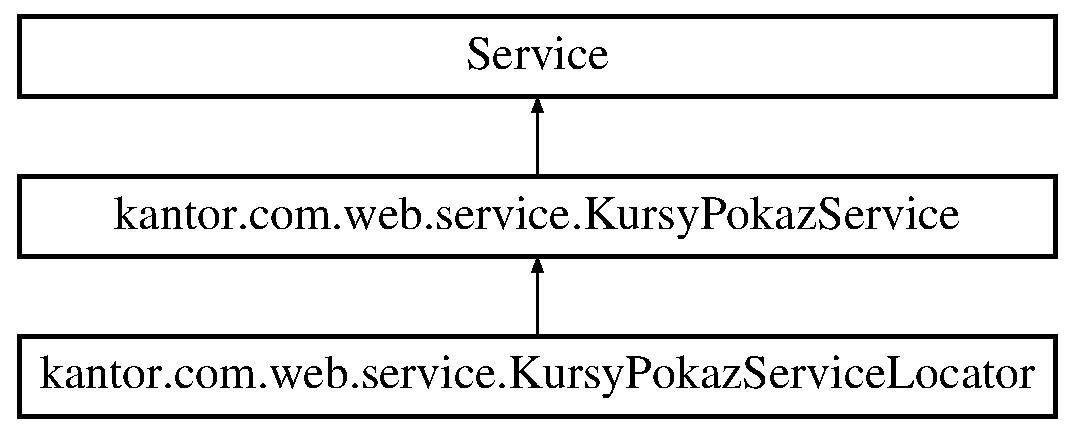
\includegraphics[height=3.000000cm]{interfacekantor_1_1com_1_1web_1_1service_1_1_kursy_pokaz_service}
\end{center}
\end{figure}
\subsection*{Public Member Functions}
\begin{DoxyCompactItemize}
\item 
java.\+lang.\+String \hyperlink{interfacekantor_1_1com_1_1web_1_1service_1_1_kursy_pokaz_service_ac0c33b447ed2b6d5824b6856f24891dd}{get\+Kursy\+Pokaz\+Address} ()
\item 
\hyperlink{classkantor_1_1com_1_1web_1_1service_1_1_kursy_pokaz}{kantor.\+com.\+web.\+service.\+Kursy\+Pokaz} \hyperlink{interfacekantor_1_1com_1_1web_1_1service_1_1_kursy_pokaz_service_aeee39cf6bfa57a840b51ad1a2b28ecce}{get\+Kursy\+Pokaz} ()  throws javax.\+xml.\+rpc.\+Service\+Exception
\item 
\hyperlink{classkantor_1_1com_1_1web_1_1service_1_1_kursy_pokaz}{kantor.\+com.\+web.\+service.\+Kursy\+Pokaz} \hyperlink{interfacekantor_1_1com_1_1web_1_1service_1_1_kursy_pokaz_service_adfdcc96d8e32882d730e05cfc8c7c263}{get\+Kursy\+Pokaz} (java.\+net.\+U\+R\+L port\+Address)  throws javax.\+xml.\+rpc.\+Service\+Exception
\end{DoxyCompactItemize}


\subsection{Detailed Description}


Definition at line 10 of file Kursy\+Pokaz\+Service.\+java.



\subsection{Member Function Documentation}
\hypertarget{interfacekantor_1_1com_1_1web_1_1service_1_1_kursy_pokaz_service_aeee39cf6bfa57a840b51ad1a2b28ecce}{\index{kantor\+::com\+::web\+::service\+::\+Kursy\+Pokaz\+Service@{kantor\+::com\+::web\+::service\+::\+Kursy\+Pokaz\+Service}!get\+Kursy\+Pokaz@{get\+Kursy\+Pokaz}}
\index{get\+Kursy\+Pokaz@{get\+Kursy\+Pokaz}!kantor\+::com\+::web\+::service\+::\+Kursy\+Pokaz\+Service@{kantor\+::com\+::web\+::service\+::\+Kursy\+Pokaz\+Service}}
\subsubsection[{get\+Kursy\+Pokaz}]{\setlength{\rightskip}{0pt plus 5cm}{\bf kantor.\+com.\+web.\+service.\+Kursy\+Pokaz} kantor.\+com.\+web.\+service.\+Kursy\+Pokaz\+Service.\+get\+Kursy\+Pokaz (
\begin{DoxyParamCaption}
{}
\end{DoxyParamCaption}
) throws javax.\+xml.\+rpc.\+Service\+Exception}}\label{interfacekantor_1_1com_1_1web_1_1service_1_1_kursy_pokaz_service_aeee39cf6bfa57a840b51ad1a2b28ecce}


Implemented in \hyperlink{classkantor_1_1com_1_1web_1_1service_1_1_kursy_pokaz_service_locator_a7b8fce52b2531330aa94743b2fd80518}{kantor.\+com.\+web.\+service.\+Kursy\+Pokaz\+Service\+Locator}.

\hypertarget{interfacekantor_1_1com_1_1web_1_1service_1_1_kursy_pokaz_service_adfdcc96d8e32882d730e05cfc8c7c263}{\index{kantor\+::com\+::web\+::service\+::\+Kursy\+Pokaz\+Service@{kantor\+::com\+::web\+::service\+::\+Kursy\+Pokaz\+Service}!get\+Kursy\+Pokaz@{get\+Kursy\+Pokaz}}
\index{get\+Kursy\+Pokaz@{get\+Kursy\+Pokaz}!kantor\+::com\+::web\+::service\+::\+Kursy\+Pokaz\+Service@{kantor\+::com\+::web\+::service\+::\+Kursy\+Pokaz\+Service}}
\subsubsection[{get\+Kursy\+Pokaz}]{\setlength{\rightskip}{0pt plus 5cm}{\bf kantor.\+com.\+web.\+service.\+Kursy\+Pokaz} kantor.\+com.\+web.\+service.\+Kursy\+Pokaz\+Service.\+get\+Kursy\+Pokaz (
\begin{DoxyParamCaption}
\item[{java.\+net.\+U\+R\+L}]{port\+Address}
\end{DoxyParamCaption}
) throws javax.\+xml.\+rpc.\+Service\+Exception}}\label{interfacekantor_1_1com_1_1web_1_1service_1_1_kursy_pokaz_service_adfdcc96d8e32882d730e05cfc8c7c263}


Implemented in \hyperlink{classkantor_1_1com_1_1web_1_1service_1_1_kursy_pokaz_service_locator_a7752a187f820619249a8ef1b6d54867d}{kantor.\+com.\+web.\+service.\+Kursy\+Pokaz\+Service\+Locator}.

\hypertarget{interfacekantor_1_1com_1_1web_1_1service_1_1_kursy_pokaz_service_ac0c33b447ed2b6d5824b6856f24891dd}{\index{kantor\+::com\+::web\+::service\+::\+Kursy\+Pokaz\+Service@{kantor\+::com\+::web\+::service\+::\+Kursy\+Pokaz\+Service}!get\+Kursy\+Pokaz\+Address@{get\+Kursy\+Pokaz\+Address}}
\index{get\+Kursy\+Pokaz\+Address@{get\+Kursy\+Pokaz\+Address}!kantor\+::com\+::web\+::service\+::\+Kursy\+Pokaz\+Service@{kantor\+::com\+::web\+::service\+::\+Kursy\+Pokaz\+Service}}
\subsubsection[{get\+Kursy\+Pokaz\+Address}]{\setlength{\rightskip}{0pt plus 5cm}java.\+lang.\+String kantor.\+com.\+web.\+service.\+Kursy\+Pokaz\+Service.\+get\+Kursy\+Pokaz\+Address (
\begin{DoxyParamCaption}
{}
\end{DoxyParamCaption}
)}}\label{interfacekantor_1_1com_1_1web_1_1service_1_1_kursy_pokaz_service_ac0c33b447ed2b6d5824b6856f24891dd}


Implemented in \hyperlink{classkantor_1_1com_1_1web_1_1service_1_1_kursy_pokaz_service_locator_acd5a6dea40341b291afd110e9fa0d151}{kantor.\+com.\+web.\+service.\+Kursy\+Pokaz\+Service\+Locator}.



The documentation for this interface was generated from the following file\+:\begin{DoxyCompactItemize}
\item 
C\+:/\+Users/kuska/\+Desktop/\+Michalik/\+K\+W/\+Kantor\+W\+S\+Client/src/kantor/com/web/service/\hyperlink{_kursy_pokaz_service_8java}{Kursy\+Pokaz\+Service.\+java}\end{DoxyCompactItemize}

\hypertarget{classkantor_1_1com_1_1web_1_1service_1_1_kursy_pokaz_service_locator}{\section{kantor.\+com.\+web.\+service.\+Kursy\+Pokaz\+Service\+Locator Class Reference}
\label{classkantor_1_1com_1_1web_1_1service_1_1_kursy_pokaz_service_locator}\index{kantor.\+com.\+web.\+service.\+Kursy\+Pokaz\+Service\+Locator@{kantor.\+com.\+web.\+service.\+Kursy\+Pokaz\+Service\+Locator}}
}
Inheritance diagram for kantor.\+com.\+web.\+service.\+Kursy\+Pokaz\+Service\+Locator\+:\begin{figure}[H]
\begin{center}
\leavevmode
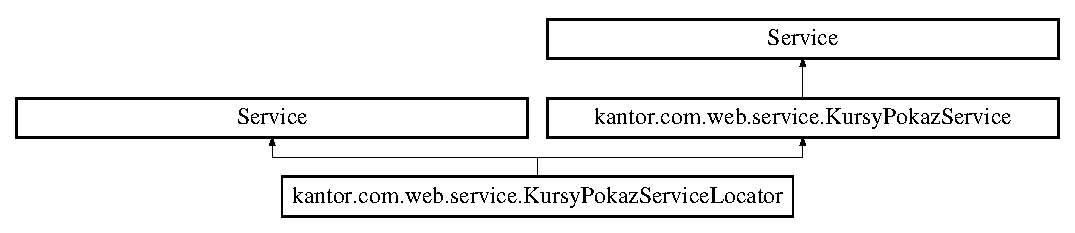
\includegraphics[height=2.683706cm]{classkantor_1_1com_1_1web_1_1service_1_1_kursy_pokaz_service_locator}
\end{center}
\end{figure}
\subsection*{Public Member Functions}
\begin{DoxyCompactItemize}
\item 
\hyperlink{classkantor_1_1com_1_1web_1_1service_1_1_kursy_pokaz_service_locator_a0d208d2392725d8949b5a5fb10158713}{Kursy\+Pokaz\+Service\+Locator} ()
\item 
\hyperlink{classkantor_1_1com_1_1web_1_1service_1_1_kursy_pokaz_service_locator_a1f352a89dc5535ba4625459762eb5306}{Kursy\+Pokaz\+Service\+Locator} (org.\+apache.\+axis.\+Engine\+Configuration config)
\item 
\hyperlink{classkantor_1_1com_1_1web_1_1service_1_1_kursy_pokaz_service_locator_aab06f25cc581463776c40370cbd8809b}{Kursy\+Pokaz\+Service\+Locator} (java.\+lang.\+String wsdl\+Loc, javax.\+xml.\+namespace.\+Q\+Name s\+Name)  throws javax.\+xml.\+rpc.\+Service\+Exception 
\item 
java.\+lang.\+String \hyperlink{classkantor_1_1com_1_1web_1_1service_1_1_kursy_pokaz_service_locator_acd5a6dea40341b291afd110e9fa0d151}{get\+Kursy\+Pokaz\+Address} ()
\item 
java.\+lang.\+String \hyperlink{classkantor_1_1com_1_1web_1_1service_1_1_kursy_pokaz_service_locator_a587b83681f721371d96d7a3497aab85c}{get\+Kursy\+Pokaz\+W\+S\+D\+D\+Service\+Name} ()
\item 
void \hyperlink{classkantor_1_1com_1_1web_1_1service_1_1_kursy_pokaz_service_locator_acd4085212ac8086417b6994413f2f5e6}{set\+Kursy\+Pokaz\+W\+S\+D\+D\+Service\+Name} (java.\+lang.\+String name)
\item 
\hyperlink{classkantor_1_1com_1_1web_1_1service_1_1_kursy_pokaz}{kantor.\+com.\+web.\+service.\+Kursy\+Pokaz} \hyperlink{classkantor_1_1com_1_1web_1_1service_1_1_kursy_pokaz_service_locator_a7b8fce52b2531330aa94743b2fd80518}{get\+Kursy\+Pokaz} ()  throws javax.\+xml.\+rpc.\+Service\+Exception 
\item 
\hyperlink{classkantor_1_1com_1_1web_1_1service_1_1_kursy_pokaz}{kantor.\+com.\+web.\+service.\+Kursy\+Pokaz} \hyperlink{classkantor_1_1com_1_1web_1_1service_1_1_kursy_pokaz_service_locator_a7752a187f820619249a8ef1b6d54867d}{get\+Kursy\+Pokaz} (java.\+net.\+U\+R\+L port\+Address)  throws javax.\+xml.\+rpc.\+Service\+Exception 
\item 
void \hyperlink{classkantor_1_1com_1_1web_1_1service_1_1_kursy_pokaz_service_locator_a4ff85e81ef5893648efc4db2ea62ee30}{set\+Kursy\+Pokaz\+Endpoint\+Address} (java.\+lang.\+String address)
\item 
java.\+rmi.\+Remote \hyperlink{classkantor_1_1com_1_1web_1_1service_1_1_kursy_pokaz_service_locator_a342d4038c3df0a6175856234f1748960}{get\+Port} (Class service\+Endpoint\+Interface)  throws javax.\+xml.\+rpc.\+Service\+Exception 
\item 
java.\+rmi.\+Remote \hyperlink{classkantor_1_1com_1_1web_1_1service_1_1_kursy_pokaz_service_locator_a848b4ee35d42a77308b8af2dfdfac21e}{get\+Port} (javax.\+xml.\+namespace.\+Q\+Name port\+Name, Class service\+Endpoint\+Interface)  throws javax.\+xml.\+rpc.\+Service\+Exception 
\item 
namespace\+::\+Q\+Name \hyperlink{classkantor_1_1com_1_1web_1_1service_1_1_kursy_pokaz_service_locator_ad766e195553030282a79619d4fe950d1}{get\+Service\+Name} ()
\item 
java.\+util.\+Iterator \hyperlink{classkantor_1_1com_1_1web_1_1service_1_1_kursy_pokaz_service_locator_a044fa9139cae5b81e520a13c15384634}{get\+Ports} ()
\item 
void \hyperlink{classkantor_1_1com_1_1web_1_1service_1_1_kursy_pokaz_service_locator_a7709d19ef1144105fa1d6006c2101fc5}{set\+Endpoint\+Address} (java.\+lang.\+String port\+Name, java.\+lang.\+String address)  throws javax.\+xml.\+rpc.\+Service\+Exception 
\item 
void \hyperlink{classkantor_1_1com_1_1web_1_1service_1_1_kursy_pokaz_service_locator_aa25f670cb43f184a2d46f4ea1e9b96cb}{set\+Endpoint\+Address} (javax.\+xml.\+namespace.\+Q\+Name port\+Name, java.\+lang.\+String address)  throws javax.\+xml.\+rpc.\+Service\+Exception 
\end{DoxyCompactItemize}


\subsection{Detailed Description}


Definition at line 10 of file Kursy\+Pokaz\+Service\+Locator.\+java.



\subsection{Constructor \& Destructor Documentation}
\hypertarget{classkantor_1_1com_1_1web_1_1service_1_1_kursy_pokaz_service_locator_a0d208d2392725d8949b5a5fb10158713}{\index{kantor\+::com\+::web\+::service\+::\+Kursy\+Pokaz\+Service\+Locator@{kantor\+::com\+::web\+::service\+::\+Kursy\+Pokaz\+Service\+Locator}!Kursy\+Pokaz\+Service\+Locator@{Kursy\+Pokaz\+Service\+Locator}}
\index{Kursy\+Pokaz\+Service\+Locator@{Kursy\+Pokaz\+Service\+Locator}!kantor\+::com\+::web\+::service\+::\+Kursy\+Pokaz\+Service\+Locator@{kantor\+::com\+::web\+::service\+::\+Kursy\+Pokaz\+Service\+Locator}}
\subsubsection[{Kursy\+Pokaz\+Service\+Locator}]{\setlength{\rightskip}{0pt plus 5cm}kantor.\+com.\+web.\+service.\+Kursy\+Pokaz\+Service\+Locator.\+Kursy\+Pokaz\+Service\+Locator (
\begin{DoxyParamCaption}
{}
\end{DoxyParamCaption}
)}}\label{classkantor_1_1com_1_1web_1_1service_1_1_kursy_pokaz_service_locator_a0d208d2392725d8949b5a5fb10158713}


Definition at line 12 of file Kursy\+Pokaz\+Service\+Locator.\+java.

\hypertarget{classkantor_1_1com_1_1web_1_1service_1_1_kursy_pokaz_service_locator_a1f352a89dc5535ba4625459762eb5306}{\index{kantor\+::com\+::web\+::service\+::\+Kursy\+Pokaz\+Service\+Locator@{kantor\+::com\+::web\+::service\+::\+Kursy\+Pokaz\+Service\+Locator}!Kursy\+Pokaz\+Service\+Locator@{Kursy\+Pokaz\+Service\+Locator}}
\index{Kursy\+Pokaz\+Service\+Locator@{Kursy\+Pokaz\+Service\+Locator}!kantor\+::com\+::web\+::service\+::\+Kursy\+Pokaz\+Service\+Locator@{kantor\+::com\+::web\+::service\+::\+Kursy\+Pokaz\+Service\+Locator}}
\subsubsection[{Kursy\+Pokaz\+Service\+Locator}]{\setlength{\rightskip}{0pt plus 5cm}kantor.\+com.\+web.\+service.\+Kursy\+Pokaz\+Service\+Locator.\+Kursy\+Pokaz\+Service\+Locator (
\begin{DoxyParamCaption}
\item[{org.\+apache.\+axis.\+Engine\+Configuration}]{config}
\end{DoxyParamCaption}
)}}\label{classkantor_1_1com_1_1web_1_1service_1_1_kursy_pokaz_service_locator_a1f352a89dc5535ba4625459762eb5306}


Definition at line 16 of file Kursy\+Pokaz\+Service\+Locator.\+java.

\hypertarget{classkantor_1_1com_1_1web_1_1service_1_1_kursy_pokaz_service_locator_aab06f25cc581463776c40370cbd8809b}{\index{kantor\+::com\+::web\+::service\+::\+Kursy\+Pokaz\+Service\+Locator@{kantor\+::com\+::web\+::service\+::\+Kursy\+Pokaz\+Service\+Locator}!Kursy\+Pokaz\+Service\+Locator@{Kursy\+Pokaz\+Service\+Locator}}
\index{Kursy\+Pokaz\+Service\+Locator@{Kursy\+Pokaz\+Service\+Locator}!kantor\+::com\+::web\+::service\+::\+Kursy\+Pokaz\+Service\+Locator@{kantor\+::com\+::web\+::service\+::\+Kursy\+Pokaz\+Service\+Locator}}
\subsubsection[{Kursy\+Pokaz\+Service\+Locator}]{\setlength{\rightskip}{0pt plus 5cm}kantor.\+com.\+web.\+service.\+Kursy\+Pokaz\+Service\+Locator.\+Kursy\+Pokaz\+Service\+Locator (
\begin{DoxyParamCaption}
\item[{java.\+lang.\+String}]{wsdl\+Loc, }
\item[{javax.\+xml.\+namespace.\+Q\+Name}]{s\+Name}
\end{DoxyParamCaption}
) throws javax.\+xml.\+rpc.\+Service\+Exception}}\label{classkantor_1_1com_1_1web_1_1service_1_1_kursy_pokaz_service_locator_aab06f25cc581463776c40370cbd8809b}


Definition at line 20 of file Kursy\+Pokaz\+Service\+Locator.\+java.



\subsection{Member Function Documentation}
\hypertarget{classkantor_1_1com_1_1web_1_1service_1_1_kursy_pokaz_service_locator_a7b8fce52b2531330aa94743b2fd80518}{\index{kantor\+::com\+::web\+::service\+::\+Kursy\+Pokaz\+Service\+Locator@{kantor\+::com\+::web\+::service\+::\+Kursy\+Pokaz\+Service\+Locator}!get\+Kursy\+Pokaz@{get\+Kursy\+Pokaz}}
\index{get\+Kursy\+Pokaz@{get\+Kursy\+Pokaz}!kantor\+::com\+::web\+::service\+::\+Kursy\+Pokaz\+Service\+Locator@{kantor\+::com\+::web\+::service\+::\+Kursy\+Pokaz\+Service\+Locator}}
\subsubsection[{get\+Kursy\+Pokaz}]{\setlength{\rightskip}{0pt plus 5cm}{\bf kantor.\+com.\+web.\+service.\+Kursy\+Pokaz} kantor.\+com.\+web.\+service.\+Kursy\+Pokaz\+Service\+Locator.\+get\+Kursy\+Pokaz (
\begin{DoxyParamCaption}
{}
\end{DoxyParamCaption}
) throws javax.\+xml.\+rpc.\+Service\+Exception}}\label{classkantor_1_1com_1_1web_1_1service_1_1_kursy_pokaz_service_locator_a7b8fce52b2531330aa94743b2fd80518}


Implements \hyperlink{interfacekantor_1_1com_1_1web_1_1service_1_1_kursy_pokaz_service_aeee39cf6bfa57a840b51ad1a2b28ecce}{kantor.\+com.\+web.\+service.\+Kursy\+Pokaz\+Service}.



Definition at line 42 of file Kursy\+Pokaz\+Service\+Locator.\+java.

\hypertarget{classkantor_1_1com_1_1web_1_1service_1_1_kursy_pokaz_service_locator_a7752a187f820619249a8ef1b6d54867d}{\index{kantor\+::com\+::web\+::service\+::\+Kursy\+Pokaz\+Service\+Locator@{kantor\+::com\+::web\+::service\+::\+Kursy\+Pokaz\+Service\+Locator}!get\+Kursy\+Pokaz@{get\+Kursy\+Pokaz}}
\index{get\+Kursy\+Pokaz@{get\+Kursy\+Pokaz}!kantor\+::com\+::web\+::service\+::\+Kursy\+Pokaz\+Service\+Locator@{kantor\+::com\+::web\+::service\+::\+Kursy\+Pokaz\+Service\+Locator}}
\subsubsection[{get\+Kursy\+Pokaz}]{\setlength{\rightskip}{0pt plus 5cm}{\bf kantor.\+com.\+web.\+service.\+Kursy\+Pokaz} kantor.\+com.\+web.\+service.\+Kursy\+Pokaz\+Service\+Locator.\+get\+Kursy\+Pokaz (
\begin{DoxyParamCaption}
\item[{java.\+net.\+U\+R\+L}]{port\+Address}
\end{DoxyParamCaption}
) throws javax.\+xml.\+rpc.\+Service\+Exception}}\label{classkantor_1_1com_1_1web_1_1service_1_1_kursy_pokaz_service_locator_a7752a187f820619249a8ef1b6d54867d}


Implements \hyperlink{interfacekantor_1_1com_1_1web_1_1service_1_1_kursy_pokaz_service_adfdcc96d8e32882d730e05cfc8c7c263}{kantor.\+com.\+web.\+service.\+Kursy\+Pokaz\+Service}.



Definition at line 53 of file Kursy\+Pokaz\+Service\+Locator.\+java.

\hypertarget{classkantor_1_1com_1_1web_1_1service_1_1_kursy_pokaz_service_locator_acd5a6dea40341b291afd110e9fa0d151}{\index{kantor\+::com\+::web\+::service\+::\+Kursy\+Pokaz\+Service\+Locator@{kantor\+::com\+::web\+::service\+::\+Kursy\+Pokaz\+Service\+Locator}!get\+Kursy\+Pokaz\+Address@{get\+Kursy\+Pokaz\+Address}}
\index{get\+Kursy\+Pokaz\+Address@{get\+Kursy\+Pokaz\+Address}!kantor\+::com\+::web\+::service\+::\+Kursy\+Pokaz\+Service\+Locator@{kantor\+::com\+::web\+::service\+::\+Kursy\+Pokaz\+Service\+Locator}}
\subsubsection[{get\+Kursy\+Pokaz\+Address}]{\setlength{\rightskip}{0pt plus 5cm}java.\+lang.\+String kantor.\+com.\+web.\+service.\+Kursy\+Pokaz\+Service\+Locator.\+get\+Kursy\+Pokaz\+Address (
\begin{DoxyParamCaption}
{}
\end{DoxyParamCaption}
)}}\label{classkantor_1_1com_1_1web_1_1service_1_1_kursy_pokaz_service_locator_acd5a6dea40341b291afd110e9fa0d151}


Implements \hyperlink{interfacekantor_1_1com_1_1web_1_1service_1_1_kursy_pokaz_service_ac0c33b447ed2b6d5824b6856f24891dd}{kantor.\+com.\+web.\+service.\+Kursy\+Pokaz\+Service}.



Definition at line 27 of file Kursy\+Pokaz\+Service\+Locator.\+java.

\hypertarget{classkantor_1_1com_1_1web_1_1service_1_1_kursy_pokaz_service_locator_a587b83681f721371d96d7a3497aab85c}{\index{kantor\+::com\+::web\+::service\+::\+Kursy\+Pokaz\+Service\+Locator@{kantor\+::com\+::web\+::service\+::\+Kursy\+Pokaz\+Service\+Locator}!get\+Kursy\+Pokaz\+W\+S\+D\+D\+Service\+Name@{get\+Kursy\+Pokaz\+W\+S\+D\+D\+Service\+Name}}
\index{get\+Kursy\+Pokaz\+W\+S\+D\+D\+Service\+Name@{get\+Kursy\+Pokaz\+W\+S\+D\+D\+Service\+Name}!kantor\+::com\+::web\+::service\+::\+Kursy\+Pokaz\+Service\+Locator@{kantor\+::com\+::web\+::service\+::\+Kursy\+Pokaz\+Service\+Locator}}
\subsubsection[{get\+Kursy\+Pokaz\+W\+S\+D\+D\+Service\+Name}]{\setlength{\rightskip}{0pt plus 5cm}java.\+lang.\+String kantor.\+com.\+web.\+service.\+Kursy\+Pokaz\+Service\+Locator.\+get\+Kursy\+Pokaz\+W\+S\+D\+D\+Service\+Name (
\begin{DoxyParamCaption}
{}
\end{DoxyParamCaption}
)}}\label{classkantor_1_1com_1_1web_1_1service_1_1_kursy_pokaz_service_locator_a587b83681f721371d96d7a3497aab85c}


Definition at line 34 of file Kursy\+Pokaz\+Service\+Locator.\+java.

\hypertarget{classkantor_1_1com_1_1web_1_1service_1_1_kursy_pokaz_service_locator_a342d4038c3df0a6175856234f1748960}{\index{kantor\+::com\+::web\+::service\+::\+Kursy\+Pokaz\+Service\+Locator@{kantor\+::com\+::web\+::service\+::\+Kursy\+Pokaz\+Service\+Locator}!get\+Port@{get\+Port}}
\index{get\+Port@{get\+Port}!kantor\+::com\+::web\+::service\+::\+Kursy\+Pokaz\+Service\+Locator@{kantor\+::com\+::web\+::service\+::\+Kursy\+Pokaz\+Service\+Locator}}
\subsubsection[{get\+Port}]{\setlength{\rightskip}{0pt plus 5cm}java.\+rmi.\+Remote kantor.\+com.\+web.\+service.\+Kursy\+Pokaz\+Service\+Locator.\+get\+Port (
\begin{DoxyParamCaption}
\item[{Class}]{service\+Endpoint\+Interface}
\end{DoxyParamCaption}
) throws javax.\+xml.\+rpc.\+Service\+Exception}}\label{classkantor_1_1com_1_1web_1_1service_1_1_kursy_pokaz_service_locator_a342d4038c3df0a6175856234f1748960}
For the given interface, get the stub implementation. If this service has no port for the given interface, then Service\+Exception is thrown. 

Definition at line 73 of file Kursy\+Pokaz\+Service\+Locator.\+java.

\hypertarget{classkantor_1_1com_1_1web_1_1service_1_1_kursy_pokaz_service_locator_a848b4ee35d42a77308b8af2dfdfac21e}{\index{kantor\+::com\+::web\+::service\+::\+Kursy\+Pokaz\+Service\+Locator@{kantor\+::com\+::web\+::service\+::\+Kursy\+Pokaz\+Service\+Locator}!get\+Port@{get\+Port}}
\index{get\+Port@{get\+Port}!kantor\+::com\+::web\+::service\+::\+Kursy\+Pokaz\+Service\+Locator@{kantor\+::com\+::web\+::service\+::\+Kursy\+Pokaz\+Service\+Locator}}
\subsubsection[{get\+Port}]{\setlength{\rightskip}{0pt plus 5cm}java.\+rmi.\+Remote kantor.\+com.\+web.\+service.\+Kursy\+Pokaz\+Service\+Locator.\+get\+Port (
\begin{DoxyParamCaption}
\item[{javax.\+xml.\+namespace.\+Q\+Name}]{port\+Name, }
\item[{Class}]{service\+Endpoint\+Interface}
\end{DoxyParamCaption}
) throws javax.\+xml.\+rpc.\+Service\+Exception}}\label{classkantor_1_1com_1_1web_1_1service_1_1_kursy_pokaz_service_locator_a848b4ee35d42a77308b8af2dfdfac21e}
For the given interface, get the stub implementation. If this service has no port for the given interface, then Service\+Exception is thrown. 

Definition at line 92 of file Kursy\+Pokaz\+Service\+Locator.\+java.

\hypertarget{classkantor_1_1com_1_1web_1_1service_1_1_kursy_pokaz_service_locator_a044fa9139cae5b81e520a13c15384634}{\index{kantor\+::com\+::web\+::service\+::\+Kursy\+Pokaz\+Service\+Locator@{kantor\+::com\+::web\+::service\+::\+Kursy\+Pokaz\+Service\+Locator}!get\+Ports@{get\+Ports}}
\index{get\+Ports@{get\+Ports}!kantor\+::com\+::web\+::service\+::\+Kursy\+Pokaz\+Service\+Locator@{kantor\+::com\+::web\+::service\+::\+Kursy\+Pokaz\+Service\+Locator}}
\subsubsection[{get\+Ports}]{\setlength{\rightskip}{0pt plus 5cm}java.\+util.\+Iterator kantor.\+com.\+web.\+service.\+Kursy\+Pokaz\+Service\+Locator.\+get\+Ports (
\begin{DoxyParamCaption}
{}
\end{DoxyParamCaption}
)}}\label{classkantor_1_1com_1_1web_1_1service_1_1_kursy_pokaz_service_locator_a044fa9139cae5b81e520a13c15384634}


Definition at line 113 of file Kursy\+Pokaz\+Service\+Locator.\+java.

\hypertarget{classkantor_1_1com_1_1web_1_1service_1_1_kursy_pokaz_service_locator_ad766e195553030282a79619d4fe950d1}{\index{kantor\+::com\+::web\+::service\+::\+Kursy\+Pokaz\+Service\+Locator@{kantor\+::com\+::web\+::service\+::\+Kursy\+Pokaz\+Service\+Locator}!get\+Service\+Name@{get\+Service\+Name}}
\index{get\+Service\+Name@{get\+Service\+Name}!kantor\+::com\+::web\+::service\+::\+Kursy\+Pokaz\+Service\+Locator@{kantor\+::com\+::web\+::service\+::\+Kursy\+Pokaz\+Service\+Locator}}
\subsubsection[{get\+Service\+Name}]{\setlength{\rightskip}{0pt plus 5cm}namespace .Q\+Name kantor.\+com.\+web.\+service.\+Kursy\+Pokaz\+Service\+Locator.\+get\+Service\+Name (
\begin{DoxyParamCaption}
{}
\end{DoxyParamCaption}
)}}\label{classkantor_1_1com_1_1web_1_1service_1_1_kursy_pokaz_service_locator_ad766e195553030282a79619d4fe950d1}


Definition at line 107 of file Kursy\+Pokaz\+Service\+Locator.\+java.

\hypertarget{classkantor_1_1com_1_1web_1_1service_1_1_kursy_pokaz_service_locator_a7709d19ef1144105fa1d6006c2101fc5}{\index{kantor\+::com\+::web\+::service\+::\+Kursy\+Pokaz\+Service\+Locator@{kantor\+::com\+::web\+::service\+::\+Kursy\+Pokaz\+Service\+Locator}!set\+Endpoint\+Address@{set\+Endpoint\+Address}}
\index{set\+Endpoint\+Address@{set\+Endpoint\+Address}!kantor\+::com\+::web\+::service\+::\+Kursy\+Pokaz\+Service\+Locator@{kantor\+::com\+::web\+::service\+::\+Kursy\+Pokaz\+Service\+Locator}}
\subsubsection[{set\+Endpoint\+Address}]{\setlength{\rightskip}{0pt plus 5cm}void kantor.\+com.\+web.\+service.\+Kursy\+Pokaz\+Service\+Locator.\+set\+Endpoint\+Address (
\begin{DoxyParamCaption}
\item[{java.\+lang.\+String}]{port\+Name, }
\item[{java.\+lang.\+String}]{address}
\end{DoxyParamCaption}
) throws javax.\+xml.\+rpc.\+Service\+Exception}}\label{classkantor_1_1com_1_1web_1_1service_1_1_kursy_pokaz_service_locator_a7709d19ef1144105fa1d6006c2101fc5}
Set the endpoint address for the specified port name. 

Definition at line 124 of file Kursy\+Pokaz\+Service\+Locator.\+java.

\hypertarget{classkantor_1_1com_1_1web_1_1service_1_1_kursy_pokaz_service_locator_aa25f670cb43f184a2d46f4ea1e9b96cb}{\index{kantor\+::com\+::web\+::service\+::\+Kursy\+Pokaz\+Service\+Locator@{kantor\+::com\+::web\+::service\+::\+Kursy\+Pokaz\+Service\+Locator}!set\+Endpoint\+Address@{set\+Endpoint\+Address}}
\index{set\+Endpoint\+Address@{set\+Endpoint\+Address}!kantor\+::com\+::web\+::service\+::\+Kursy\+Pokaz\+Service\+Locator@{kantor\+::com\+::web\+::service\+::\+Kursy\+Pokaz\+Service\+Locator}}
\subsubsection[{set\+Endpoint\+Address}]{\setlength{\rightskip}{0pt plus 5cm}void kantor.\+com.\+web.\+service.\+Kursy\+Pokaz\+Service\+Locator.\+set\+Endpoint\+Address (
\begin{DoxyParamCaption}
\item[{javax.\+xml.\+namespace.\+Q\+Name}]{port\+Name, }
\item[{java.\+lang.\+String}]{address}
\end{DoxyParamCaption}
) throws javax.\+xml.\+rpc.\+Service\+Exception}}\label{classkantor_1_1com_1_1web_1_1service_1_1_kursy_pokaz_service_locator_aa25f670cb43f184a2d46f4ea1e9b96cb}
Set the endpoint address for the specified port name. 

Definition at line 138 of file Kursy\+Pokaz\+Service\+Locator.\+java.

\hypertarget{classkantor_1_1com_1_1web_1_1service_1_1_kursy_pokaz_service_locator_a4ff85e81ef5893648efc4db2ea62ee30}{\index{kantor\+::com\+::web\+::service\+::\+Kursy\+Pokaz\+Service\+Locator@{kantor\+::com\+::web\+::service\+::\+Kursy\+Pokaz\+Service\+Locator}!set\+Kursy\+Pokaz\+Endpoint\+Address@{set\+Kursy\+Pokaz\+Endpoint\+Address}}
\index{set\+Kursy\+Pokaz\+Endpoint\+Address@{set\+Kursy\+Pokaz\+Endpoint\+Address}!kantor\+::com\+::web\+::service\+::\+Kursy\+Pokaz\+Service\+Locator@{kantor\+::com\+::web\+::service\+::\+Kursy\+Pokaz\+Service\+Locator}}
\subsubsection[{set\+Kursy\+Pokaz\+Endpoint\+Address}]{\setlength{\rightskip}{0pt plus 5cm}void kantor.\+com.\+web.\+service.\+Kursy\+Pokaz\+Service\+Locator.\+set\+Kursy\+Pokaz\+Endpoint\+Address (
\begin{DoxyParamCaption}
\item[{java.\+lang.\+String}]{address}
\end{DoxyParamCaption}
)}}\label{classkantor_1_1com_1_1web_1_1service_1_1_kursy_pokaz_service_locator_a4ff85e81ef5893648efc4db2ea62ee30}


Definition at line 64 of file Kursy\+Pokaz\+Service\+Locator.\+java.

\hypertarget{classkantor_1_1com_1_1web_1_1service_1_1_kursy_pokaz_service_locator_acd4085212ac8086417b6994413f2f5e6}{\index{kantor\+::com\+::web\+::service\+::\+Kursy\+Pokaz\+Service\+Locator@{kantor\+::com\+::web\+::service\+::\+Kursy\+Pokaz\+Service\+Locator}!set\+Kursy\+Pokaz\+W\+S\+D\+D\+Service\+Name@{set\+Kursy\+Pokaz\+W\+S\+D\+D\+Service\+Name}}
\index{set\+Kursy\+Pokaz\+W\+S\+D\+D\+Service\+Name@{set\+Kursy\+Pokaz\+W\+S\+D\+D\+Service\+Name}!kantor\+::com\+::web\+::service\+::\+Kursy\+Pokaz\+Service\+Locator@{kantor\+::com\+::web\+::service\+::\+Kursy\+Pokaz\+Service\+Locator}}
\subsubsection[{set\+Kursy\+Pokaz\+W\+S\+D\+D\+Service\+Name}]{\setlength{\rightskip}{0pt plus 5cm}void kantor.\+com.\+web.\+service.\+Kursy\+Pokaz\+Service\+Locator.\+set\+Kursy\+Pokaz\+W\+S\+D\+D\+Service\+Name (
\begin{DoxyParamCaption}
\item[{java.\+lang.\+String}]{name}
\end{DoxyParamCaption}
)}}\label{classkantor_1_1com_1_1web_1_1service_1_1_kursy_pokaz_service_locator_acd4085212ac8086417b6994413f2f5e6}


Definition at line 38 of file Kursy\+Pokaz\+Service\+Locator.\+java.



The documentation for this class was generated from the following file\+:\begin{DoxyCompactItemize}
\item 
C\+:/\+Users/kuska/\+Desktop/\+Michalik/\+K\+W/\+Kantor\+W\+S\+Client/src/kantor/com/web/service/\hyperlink{_kursy_pokaz_service_locator_8java}{Kursy\+Pokaz\+Service\+Locator.\+java}\end{DoxyCompactItemize}

\hypertarget{classkantor_1_1com_1_1web_1_1service_1_1_kursy_pokaz_soap_binding_stub}{\section{kantor.\+com.\+web.\+service.\+Kursy\+Pokaz\+Soap\+Binding\+Stub Class Reference}
\label{classkantor_1_1com_1_1web_1_1service_1_1_kursy_pokaz_soap_binding_stub}\index{kantor.\+com.\+web.\+service.\+Kursy\+Pokaz\+Soap\+Binding\+Stub@{kantor.\+com.\+web.\+service.\+Kursy\+Pokaz\+Soap\+Binding\+Stub}}
}
Inheritance diagram for kantor.\+com.\+web.\+service.\+Kursy\+Pokaz\+Soap\+Binding\+Stub\+:\begin{figure}[H]
\begin{center}
\leavevmode
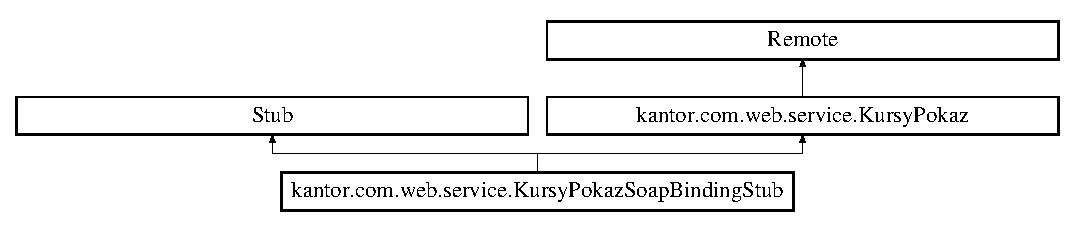
\includegraphics[height=2.608696cm]{classkantor_1_1com_1_1web_1_1service_1_1_kursy_pokaz_soap_binding_stub}
\end{center}
\end{figure}
\subsection*{Public Member Functions}
\begin{DoxyCompactItemize}
\item 
\hyperlink{classkantor_1_1com_1_1web_1_1service_1_1_kursy_pokaz_soap_binding_stub_aec58f518269c22a2c0c006966e07bace}{Kursy\+Pokaz\+Soap\+Binding\+Stub} ()  throws org.\+apache.\+axis.\+Axis\+Fault 
\item 
\hyperlink{classkantor_1_1com_1_1web_1_1service_1_1_kursy_pokaz_soap_binding_stub_a5d6d3b8257a8f09803deb90b3c6b79c0}{Kursy\+Pokaz\+Soap\+Binding\+Stub} (java.\+net.\+U\+R\+L endpoint\+U\+R\+L, javax.\+xml.\+rpc.\+Service service)  throws org.\+apache.\+axis.\+Axis\+Fault 
\item 
\hyperlink{classkantor_1_1com_1_1web_1_1service_1_1_kursy_pokaz_soap_binding_stub_aac01c798f0276a9eb2132a01e5bb1615}{Kursy\+Pokaz\+Soap\+Binding\+Stub} (javax.\+xml.\+rpc.\+Service service)  throws org.\+apache.\+axis.\+Axis\+Fault 
\item 
double \hyperlink{classkantor_1_1com_1_1web_1_1service_1_1_kursy_pokaz_soap_binding_stub_a3e89646ddaed6b605071d1f6d186e66e}{E\+U\+Rna\+P\+L\+N} ()  throws java.\+rmi.\+Remote\+Exception 
\item 
double \hyperlink{classkantor_1_1com_1_1web_1_1service_1_1_kursy_pokaz_soap_binding_stub_a6dd0efcbf660c065637f49570889f41d}{P\+L\+Nna\+E\+U\+R} ()  throws java.\+rmi.\+Remote\+Exception 
\item 
double \hyperlink{classkantor_1_1com_1_1web_1_1service_1_1_kursy_pokaz_soap_binding_stub_a2f975ee29635758cd503316c16ba179c}{P\+L\+Nna\+U\+S\+D} ()  throws java.\+rmi.\+Remote\+Exception 
\item 
double \hyperlink{classkantor_1_1com_1_1web_1_1service_1_1_kursy_pokaz_soap_binding_stub_aa8b296ac90b4ab4c880652527c013db2}{U\+S\+Dna\+P\+L\+N} ()  throws java.\+rmi.\+Remote\+Exception 
\end{DoxyCompactItemize}
\subsection*{Protected Member Functions}
\begin{DoxyCompactItemize}
\item 
org.\+apache.\+axis.\+client.\+Call \hyperlink{classkantor_1_1com_1_1web_1_1service_1_1_kursy_pokaz_soap_binding_stub_abf9955a7397853953430fbbba1ecd88f}{create\+Call} ()  throws java.\+rmi.\+Remote\+Exception 
\end{DoxyCompactItemize}


\subsection{Detailed Description}


Definition at line 10 of file Kursy\+Pokaz\+Soap\+Binding\+Stub.\+java.



\subsection{Constructor \& Destructor Documentation}
\hypertarget{classkantor_1_1com_1_1web_1_1service_1_1_kursy_pokaz_soap_binding_stub_aec58f518269c22a2c0c006966e07bace}{\index{kantor\+::com\+::web\+::service\+::\+Kursy\+Pokaz\+Soap\+Binding\+Stub@{kantor\+::com\+::web\+::service\+::\+Kursy\+Pokaz\+Soap\+Binding\+Stub}!Kursy\+Pokaz\+Soap\+Binding\+Stub@{Kursy\+Pokaz\+Soap\+Binding\+Stub}}
\index{Kursy\+Pokaz\+Soap\+Binding\+Stub@{Kursy\+Pokaz\+Soap\+Binding\+Stub}!kantor\+::com\+::web\+::service\+::\+Kursy\+Pokaz\+Soap\+Binding\+Stub@{kantor\+::com\+::web\+::service\+::\+Kursy\+Pokaz\+Soap\+Binding\+Stub}}
\subsubsection[{Kursy\+Pokaz\+Soap\+Binding\+Stub}]{\setlength{\rightskip}{0pt plus 5cm}kantor.\+com.\+web.\+service.\+Kursy\+Pokaz\+Soap\+Binding\+Stub.\+Kursy\+Pokaz\+Soap\+Binding\+Stub (
\begin{DoxyParamCaption}
{}
\end{DoxyParamCaption}
) throws org.\+apache.\+axis.\+Axis\+Fault}}\label{classkantor_1_1com_1_1web_1_1service_1_1_kursy_pokaz_soap_binding_stub_aec58f518269c22a2c0c006966e07bace}


Definition at line 64 of file Kursy\+Pokaz\+Soap\+Binding\+Stub.\+java.

\hypertarget{classkantor_1_1com_1_1web_1_1service_1_1_kursy_pokaz_soap_binding_stub_a5d6d3b8257a8f09803deb90b3c6b79c0}{\index{kantor\+::com\+::web\+::service\+::\+Kursy\+Pokaz\+Soap\+Binding\+Stub@{kantor\+::com\+::web\+::service\+::\+Kursy\+Pokaz\+Soap\+Binding\+Stub}!Kursy\+Pokaz\+Soap\+Binding\+Stub@{Kursy\+Pokaz\+Soap\+Binding\+Stub}}
\index{Kursy\+Pokaz\+Soap\+Binding\+Stub@{Kursy\+Pokaz\+Soap\+Binding\+Stub}!kantor\+::com\+::web\+::service\+::\+Kursy\+Pokaz\+Soap\+Binding\+Stub@{kantor\+::com\+::web\+::service\+::\+Kursy\+Pokaz\+Soap\+Binding\+Stub}}
\subsubsection[{Kursy\+Pokaz\+Soap\+Binding\+Stub}]{\setlength{\rightskip}{0pt plus 5cm}kantor.\+com.\+web.\+service.\+Kursy\+Pokaz\+Soap\+Binding\+Stub.\+Kursy\+Pokaz\+Soap\+Binding\+Stub (
\begin{DoxyParamCaption}
\item[{java.\+net.\+U\+R\+L}]{endpoint\+U\+R\+L, }
\item[{javax.\+xml.\+rpc.\+Service}]{service}
\end{DoxyParamCaption}
) throws org.\+apache.\+axis.\+Axis\+Fault}}\label{classkantor_1_1com_1_1web_1_1service_1_1_kursy_pokaz_soap_binding_stub_a5d6d3b8257a8f09803deb90b3c6b79c0}


Definition at line 68 of file Kursy\+Pokaz\+Soap\+Binding\+Stub.\+java.

\hypertarget{classkantor_1_1com_1_1web_1_1service_1_1_kursy_pokaz_soap_binding_stub_aac01c798f0276a9eb2132a01e5bb1615}{\index{kantor\+::com\+::web\+::service\+::\+Kursy\+Pokaz\+Soap\+Binding\+Stub@{kantor\+::com\+::web\+::service\+::\+Kursy\+Pokaz\+Soap\+Binding\+Stub}!Kursy\+Pokaz\+Soap\+Binding\+Stub@{Kursy\+Pokaz\+Soap\+Binding\+Stub}}
\index{Kursy\+Pokaz\+Soap\+Binding\+Stub@{Kursy\+Pokaz\+Soap\+Binding\+Stub}!kantor\+::com\+::web\+::service\+::\+Kursy\+Pokaz\+Soap\+Binding\+Stub@{kantor\+::com\+::web\+::service\+::\+Kursy\+Pokaz\+Soap\+Binding\+Stub}}
\subsubsection[{Kursy\+Pokaz\+Soap\+Binding\+Stub}]{\setlength{\rightskip}{0pt plus 5cm}kantor.\+com.\+web.\+service.\+Kursy\+Pokaz\+Soap\+Binding\+Stub.\+Kursy\+Pokaz\+Soap\+Binding\+Stub (
\begin{DoxyParamCaption}
\item[{javax.\+xml.\+rpc.\+Service}]{service}
\end{DoxyParamCaption}
) throws org.\+apache.\+axis.\+Axis\+Fault}}\label{classkantor_1_1com_1_1web_1_1service_1_1_kursy_pokaz_soap_binding_stub_aac01c798f0276a9eb2132a01e5bb1615}


Definition at line 73 of file Kursy\+Pokaz\+Soap\+Binding\+Stub.\+java.



\subsection{Member Function Documentation}
\hypertarget{classkantor_1_1com_1_1web_1_1service_1_1_kursy_pokaz_soap_binding_stub_abf9955a7397853953430fbbba1ecd88f}{\index{kantor\+::com\+::web\+::service\+::\+Kursy\+Pokaz\+Soap\+Binding\+Stub@{kantor\+::com\+::web\+::service\+::\+Kursy\+Pokaz\+Soap\+Binding\+Stub}!create\+Call@{create\+Call}}
\index{create\+Call@{create\+Call}!kantor\+::com\+::web\+::service\+::\+Kursy\+Pokaz\+Soap\+Binding\+Stub@{kantor\+::com\+::web\+::service\+::\+Kursy\+Pokaz\+Soap\+Binding\+Stub}}
\subsubsection[{create\+Call}]{\setlength{\rightskip}{0pt plus 5cm}org.\+apache.\+axis.\+client.\+Call kantor.\+com.\+web.\+service.\+Kursy\+Pokaz\+Soap\+Binding\+Stub.\+create\+Call (
\begin{DoxyParamCaption}
{}
\end{DoxyParamCaption}
) throws java.\+rmi.\+Remote\+Exception\hspace{0.3cm}{\ttfamily [protected]}}}\label{classkantor_1_1com_1_1web_1_1service_1_1_kursy_pokaz_soap_binding_stub_abf9955a7397853953430fbbba1ecd88f}


Definition at line 82 of file Kursy\+Pokaz\+Soap\+Binding\+Stub.\+java.

\hypertarget{classkantor_1_1com_1_1web_1_1service_1_1_kursy_pokaz_soap_binding_stub_a3e89646ddaed6b605071d1f6d186e66e}{\index{kantor\+::com\+::web\+::service\+::\+Kursy\+Pokaz\+Soap\+Binding\+Stub@{kantor\+::com\+::web\+::service\+::\+Kursy\+Pokaz\+Soap\+Binding\+Stub}!E\+U\+Rna\+P\+L\+N@{E\+U\+Rna\+P\+L\+N}}
\index{E\+U\+Rna\+P\+L\+N@{E\+U\+Rna\+P\+L\+N}!kantor\+::com\+::web\+::service\+::\+Kursy\+Pokaz\+Soap\+Binding\+Stub@{kantor\+::com\+::web\+::service\+::\+Kursy\+Pokaz\+Soap\+Binding\+Stub}}
\subsubsection[{E\+U\+Rna\+P\+L\+N}]{\setlength{\rightskip}{0pt plus 5cm}double kantor.\+com.\+web.\+service.\+Kursy\+Pokaz\+Soap\+Binding\+Stub.\+E\+U\+Rna\+P\+L\+N (
\begin{DoxyParamCaption}
{}
\end{DoxyParamCaption}
) throws java.\+rmi.\+Remote\+Exception}}\label{classkantor_1_1com_1_1web_1_1service_1_1_kursy_pokaz_soap_binding_stub_a3e89646ddaed6b605071d1f6d186e66e}


Implements \hyperlink{classkantor_1_1com_1_1web_1_1service_1_1_kursy_pokaz_a31eef9def09b0841facda085644ede65}{kantor.\+com.\+web.\+service.\+Kursy\+Pokaz}.



Definition at line 115 of file Kursy\+Pokaz\+Soap\+Binding\+Stub.\+java.

\hypertarget{classkantor_1_1com_1_1web_1_1service_1_1_kursy_pokaz_soap_binding_stub_a6dd0efcbf660c065637f49570889f41d}{\index{kantor\+::com\+::web\+::service\+::\+Kursy\+Pokaz\+Soap\+Binding\+Stub@{kantor\+::com\+::web\+::service\+::\+Kursy\+Pokaz\+Soap\+Binding\+Stub}!P\+L\+Nna\+E\+U\+R@{P\+L\+Nna\+E\+U\+R}}
\index{P\+L\+Nna\+E\+U\+R@{P\+L\+Nna\+E\+U\+R}!kantor\+::com\+::web\+::service\+::\+Kursy\+Pokaz\+Soap\+Binding\+Stub@{kantor\+::com\+::web\+::service\+::\+Kursy\+Pokaz\+Soap\+Binding\+Stub}}
\subsubsection[{P\+L\+Nna\+E\+U\+R}]{\setlength{\rightskip}{0pt plus 5cm}double kantor.\+com.\+web.\+service.\+Kursy\+Pokaz\+Soap\+Binding\+Stub.\+P\+L\+Nna\+E\+U\+R (
\begin{DoxyParamCaption}
{}
\end{DoxyParamCaption}
) throws java.\+rmi.\+Remote\+Exception}}\label{classkantor_1_1com_1_1web_1_1service_1_1_kursy_pokaz_soap_binding_stub_a6dd0efcbf660c065637f49570889f41d}


Implements \hyperlink{classkantor_1_1com_1_1web_1_1service_1_1_kursy_pokaz_a758e416bdc0cdec7848747c2ceb5818e}{kantor.\+com.\+web.\+service.\+Kursy\+Pokaz}.



Definition at line 149 of file Kursy\+Pokaz\+Soap\+Binding\+Stub.\+java.

\hypertarget{classkantor_1_1com_1_1web_1_1service_1_1_kursy_pokaz_soap_binding_stub_a2f975ee29635758cd503316c16ba179c}{\index{kantor\+::com\+::web\+::service\+::\+Kursy\+Pokaz\+Soap\+Binding\+Stub@{kantor\+::com\+::web\+::service\+::\+Kursy\+Pokaz\+Soap\+Binding\+Stub}!P\+L\+Nna\+U\+S\+D@{P\+L\+Nna\+U\+S\+D}}
\index{P\+L\+Nna\+U\+S\+D@{P\+L\+Nna\+U\+S\+D}!kantor\+::com\+::web\+::service\+::\+Kursy\+Pokaz\+Soap\+Binding\+Stub@{kantor\+::com\+::web\+::service\+::\+Kursy\+Pokaz\+Soap\+Binding\+Stub}}
\subsubsection[{P\+L\+Nna\+U\+S\+D}]{\setlength{\rightskip}{0pt plus 5cm}double kantor.\+com.\+web.\+service.\+Kursy\+Pokaz\+Soap\+Binding\+Stub.\+P\+L\+Nna\+U\+S\+D (
\begin{DoxyParamCaption}
{}
\end{DoxyParamCaption}
) throws java.\+rmi.\+Remote\+Exception}}\label{classkantor_1_1com_1_1web_1_1service_1_1_kursy_pokaz_soap_binding_stub_a2f975ee29635758cd503316c16ba179c}


Implements \hyperlink{classkantor_1_1com_1_1web_1_1service_1_1_kursy_pokaz_a26efb7c3127847ac0bd6adf865c4b891}{kantor.\+com.\+web.\+service.\+Kursy\+Pokaz}.



Definition at line 183 of file Kursy\+Pokaz\+Soap\+Binding\+Stub.\+java.

\hypertarget{classkantor_1_1com_1_1web_1_1service_1_1_kursy_pokaz_soap_binding_stub_aa8b296ac90b4ab4c880652527c013db2}{\index{kantor\+::com\+::web\+::service\+::\+Kursy\+Pokaz\+Soap\+Binding\+Stub@{kantor\+::com\+::web\+::service\+::\+Kursy\+Pokaz\+Soap\+Binding\+Stub}!U\+S\+Dna\+P\+L\+N@{U\+S\+Dna\+P\+L\+N}}
\index{U\+S\+Dna\+P\+L\+N@{U\+S\+Dna\+P\+L\+N}!kantor\+::com\+::web\+::service\+::\+Kursy\+Pokaz\+Soap\+Binding\+Stub@{kantor\+::com\+::web\+::service\+::\+Kursy\+Pokaz\+Soap\+Binding\+Stub}}
\subsubsection[{U\+S\+Dna\+P\+L\+N}]{\setlength{\rightskip}{0pt plus 5cm}double kantor.\+com.\+web.\+service.\+Kursy\+Pokaz\+Soap\+Binding\+Stub.\+U\+S\+Dna\+P\+L\+N (
\begin{DoxyParamCaption}
{}
\end{DoxyParamCaption}
) throws java.\+rmi.\+Remote\+Exception}}\label{classkantor_1_1com_1_1web_1_1service_1_1_kursy_pokaz_soap_binding_stub_aa8b296ac90b4ab4c880652527c013db2}


Implements \hyperlink{classkantor_1_1com_1_1web_1_1service_1_1_kursy_pokaz_a2c8884d959ed13948edc408b94083b95}{kantor.\+com.\+web.\+service.\+Kursy\+Pokaz}.



Definition at line 217 of file Kursy\+Pokaz\+Soap\+Binding\+Stub.\+java.



The documentation for this class was generated from the following file\+:\begin{DoxyCompactItemize}
\item 
C\+:/\+Users/kuska/\+Desktop/\+Michalik/\+K\+W/\+Kantor\+W\+S\+Client/src/kantor/com/web/service/\hyperlink{_kursy_pokaz_soap_binding_stub_8java}{Kursy\+Pokaz\+Soap\+Binding\+Stub.\+java}\end{DoxyCompactItemize}

\chapter{File Documentation}
\hypertarget{dynsections_8js}{\section{C\+:/\+Users/kuska/\+Desktop/\+Michalik/\+K\+W/html/dynsections.js File Reference}
\label{dynsections_8js}\index{C\+:/\+Users/kuska/\+Desktop/\+Michalik/\+K\+W/html/dynsections.\+js@{C\+:/\+Users/kuska/\+Desktop/\+Michalik/\+K\+W/html/dynsections.\+js}}
}
\subsection*{Functions}
\begin{DoxyCompactItemize}
\item 
function \hyperlink{dynsections_8js_a1922c462474df7dfd18741c961d59a25}{toggle\+Visibility} (link\+Obj)
\item 
function \hyperlink{dynsections_8js_a8f7493ad859d4fbf2523917511ee7177}{update\+Stripes} ()
\item 
function \hyperlink{dynsections_8js_a19f577cc1ba571396a85bb1f48bf4df2}{toggle\+Level} (level)
\item 
function \hyperlink{dynsections_8js_af244da4527af2d845dca04f5656376cd}{toggle\+Folder} (id)
\item 
function \hyperlink{dynsections_8js_ac057b640b17ff32af11ced151c9305b4}{toggle\+Inherit} (id)
\end{DoxyCompactItemize}


\subsection{Function Documentation}
\hypertarget{dynsections_8js_af244da4527af2d845dca04f5656376cd}{\index{dynsections.\+js@{dynsections.\+js}!toggle\+Folder@{toggle\+Folder}}
\index{toggle\+Folder@{toggle\+Folder}!dynsections.\+js@{dynsections.\+js}}
\subsubsection[{toggle\+Folder}]{\setlength{\rightskip}{0pt plus 5cm}function toggle\+Folder (
\begin{DoxyParamCaption}
\item[{}]{id}
\end{DoxyParamCaption}
)}}\label{dynsections_8js_af244da4527af2d845dca04f5656376cd}


Definition at line 49 of file dynsections.\+js.

\hypertarget{dynsections_8js_ac057b640b17ff32af11ced151c9305b4}{\index{dynsections.\+js@{dynsections.\+js}!toggle\+Inherit@{toggle\+Inherit}}
\index{toggle\+Inherit@{toggle\+Inherit}!dynsections.\+js@{dynsections.\+js}}
\subsubsection[{toggle\+Inherit}]{\setlength{\rightskip}{0pt plus 5cm}function toggle\+Inherit (
\begin{DoxyParamCaption}
\item[{}]{id}
\end{DoxyParamCaption}
)}}\label{dynsections_8js_ac057b640b17ff32af11ced151c9305b4}


Definition at line 84 of file dynsections.\+js.

\hypertarget{dynsections_8js_a19f577cc1ba571396a85bb1f48bf4df2}{\index{dynsections.\+js@{dynsections.\+js}!toggle\+Level@{toggle\+Level}}
\index{toggle\+Level@{toggle\+Level}!dynsections.\+js@{dynsections.\+js}}
\subsubsection[{toggle\+Level}]{\setlength{\rightskip}{0pt plus 5cm}function toggle\+Level (
\begin{DoxyParamCaption}
\item[{}]{level}
\end{DoxyParamCaption}
)}}\label{dynsections_8js_a19f577cc1ba571396a85bb1f48bf4df2}


Definition at line 28 of file dynsections.\+js.

\hypertarget{dynsections_8js_a1922c462474df7dfd18741c961d59a25}{\index{dynsections.\+js@{dynsections.\+js}!toggle\+Visibility@{toggle\+Visibility}}
\index{toggle\+Visibility@{toggle\+Visibility}!dynsections.\+js@{dynsections.\+js}}
\subsubsection[{toggle\+Visibility}]{\setlength{\rightskip}{0pt plus 5cm}function toggle\+Visibility (
\begin{DoxyParamCaption}
\item[{}]{link\+Obj}
\end{DoxyParamCaption}
)}}\label{dynsections_8js_a1922c462474df7dfd18741c961d59a25}


Definition at line 1 of file dynsections.\+js.

\hypertarget{dynsections_8js_a8f7493ad859d4fbf2523917511ee7177}{\index{dynsections.\+js@{dynsections.\+js}!update\+Stripes@{update\+Stripes}}
\index{update\+Stripes@{update\+Stripes}!dynsections.\+js@{dynsections.\+js}}
\subsubsection[{update\+Stripes}]{\setlength{\rightskip}{0pt plus 5cm}function update\+Stripes (
\begin{DoxyParamCaption}
{}
\end{DoxyParamCaption}
)}}\label{dynsections_8js_a8f7493ad859d4fbf2523917511ee7177}


Definition at line 22 of file dynsections.\+js.


\hypertarget{jquery_8js}{\section{C\+:/\+Users/kuska/\+Desktop/\+Michalik/\+K\+W/html/jquery.js File Reference}
\label{jquery_8js}\index{C\+:/\+Users/kuska/\+Desktop/\+Michalik/\+K\+W/html/jquery.\+js@{C\+:/\+Users/kuska/\+Desktop/\+Michalik/\+K\+W/html/jquery.\+js}}
}
\subsection*{Functions}
\begin{DoxyCompactItemize}
\item 
\hyperlink{jquery_8js_a2fa551895933fae935a0a6b87282241d}{b} \hyperlink{jquery_8js_ad0188a1a0e382f892522cfb7dafcc937}{extend} (\{css\+Hooks\+:\{opacity\+:\{get\+:function(bw, bv)\{\hyperlink{jquery_8js_ab5582cce20b35070b73869356a852365}{if}(bv)\{var e=\hyperlink{jquery_8js_adc18d83abfd9f87d396e8fd6b6ac0fe1}{Z}(bw,\char`\"{}opacity\char`\"{},\char`\"{}opacity\char`\"{});return e===\char`\"{}\char`\"{}?\char`\"{}1\char`\"{}\+:e\}\hyperlink{jquery_8js_a0544c3fe466e421738dae463968b70ba}{else}\{return bw.\+style.\+opacity\}\}\}\}, css\+Number\+:\{fill\+Opacity\+:true, font\+Weight\+:true, line\+Height\+:true, opacity\+:true, orphans\+:true, widows\+:true, z\+Index\+:true, zoom\+:true\}, css\+Props\+:\{\char`\"{}float\char`\"{}\+:b.\+support.\+css\+Float?\char`\"{}css\+Float\char`\"{}\+:\char`\"{}style\+Float\char`\"{}\}, style\+:function(bx, bw, b\+D, by)\{\hyperlink{jquery_8js_ab5582cce20b35070b73869356a852365}{if}(!bx$\vert$$\vert$bx.\+node\+Type===3$\vert$$\vert$bx.\+node\+Type===8$\vert$$\vert$!bx.\+style)\{return\}var b\+B, b\+C, bz=b.\+camel\+Case(bw), bv=bx.\+style, b\+E=b.\+css\+Hooks\mbox{[}bz\mbox{]};bw=b.\+css\+Props\mbox{[}bz\mbox{]}$\vert$$\vert$bz;\hyperlink{jquery_8js_ab5582cce20b35070b73869356a852365}{if}(b\+D!==\hyperlink{jquery_8js_a38ee4c0b5f4fe2a18d0c783af540d253}{L})\{b\+C=typeof b\+D;\hyperlink{jquery_8js_ab5582cce20b35070b73869356a852365}{if}(b\+C===\char`\"{}string\char`\"{}\&\&(b\+B=I.\+exec(b\+D)))\{b\+D=(+(b\+B\mbox{[}1\mbox{]}+1)$\ast$+b\+B\mbox{[}2\mbox{]})+parse\+Float(\hyperlink{jquery_8js_a89ad527fcd82c01ebb587332f5b4fcd4}{b.\+css}(bx, bw));b\+C=\char`\"{}number\char`\"{}\}if(b\+D==null$\vert$$\vert$b\+C===\char`\"{}number\char`\"{}\&\&is\+Na\+N(b\+D))\{return\}\hyperlink{jquery_8js_ab5582cce20b35070b73869356a852365}{if}(b\+C===\char`\"{}number\char`\"{}\&\&!b.\+css\+Number\mbox{[}bz\mbox{]})\{b\+D+=\char`\"{}px\char`\"{}\}if(!b\+E$\vert$$\vert$!(\char`\"{}set\char`\"{}in b\+E)$\vert$$\vert$(b\+D=b\+E.\+set(bx, b\+D))!==\hyperlink{jquery_8js_a38ee4c0b5f4fe2a18d0c783af540d253}{L})\{try\{bv\mbox{[}bw\mbox{]}=b\+D\}catch(b\+A)\{\}\}\}\hyperlink{jquery_8js_a0544c3fe466e421738dae463968b70ba}{else}\{\hyperlink{jquery_8js_ab5582cce20b35070b73869356a852365}{if}(b\+E \&\&\char`\"{}get\char`\"{}in b\+E \&\&(b\+B=b\+E.\+get(bx, false, by))!==\hyperlink{jquery_8js_a38ee4c0b5f4fe2a18d0c783af540d253}{L})\{return b\+B\}return bv\mbox{[}bw\mbox{]}\}\}, css\+:function(by, bx, bv)\{var bw, e;bx=b.\+camel\+Case(bx);e=b.\+css\+Hooks\mbox{[}bx\mbox{]};bx=b.\+css\+Props\mbox{[}bx\mbox{]}$\vert$$\vert$bx;\hyperlink{jquery_8js_ab5582cce20b35070b73869356a852365}{if}(bx===\char`\"{}css\+Float\char`\"{})\{bx=\char`\"{}float\char`\"{}\}if(e \&\&\char`\"{}get\char`\"{}in e \&\&(bw=e.\+get(by, true, bv))!==\hyperlink{jquery_8js_a38ee4c0b5f4fe2a18d0c783af540d253}{L})\{return bw\}\hyperlink{jquery_8js_a0544c3fe466e421738dae463968b70ba}{else}\{\hyperlink{jquery_8js_ab5582cce20b35070b73869356a852365}{if}(\hyperlink{jquery_8js_adc18d83abfd9f87d396e8fd6b6ac0fe1}{Z})\{return \hyperlink{jquery_8js_adc18d83abfd9f87d396e8fd6b6ac0fe1}{Z}(by, bx)\}\}\}, swap\+:function(bx, bw, by)\{var e=\{\};for(var bv in bw)\{e\mbox{[}bv\mbox{]}=bx.\+style\mbox{[}bv\mbox{]};bx.\+style\mbox{[}bv\mbox{]}=bw\mbox{[}bv\mbox{]}\}by.\+call(bx);for(bv in bw)\{bx.\+style\mbox{[}bv\mbox{]}=e\mbox{[}bv\mbox{]}\}\}\})
\item 
\hyperlink{jquery_8js_a2fa551895933fae935a0a6b87282241d}{b} \hyperlink{jquery_8js_a871ff39db627c54c710a3e9909b8234c}{each} (\mbox{[}\char`\"{}height\char`\"{},\char`\"{}width\char`\"{}\mbox{]}, function(bv, e)\{b.\+css\+Hooks\mbox{[}e\mbox{]}=\{get\+:function(by, bx, bw)\{var bz;\hyperlink{jquery_8js_ab5582cce20b35070b73869356a852365}{if}(bx)\{\hyperlink{jquery_8js_ab5582cce20b35070b73869356a852365}{if}(by.\+offset\+Width!==0)\{return \hyperlink{jquery_8js_a2335e57f79b6acfb6de59c235dc8a83e}{p}(by, e, bw)\}\hyperlink{jquery_8js_a0544c3fe466e421738dae463968b70ba}{else}\{b.\+swap(by, a7, function()\{bz=\hyperlink{jquery_8js_a2335e57f79b6acfb6de59c235dc8a83e}{p}(by, e, bw)\})\}return bz\}\}, set\+:function(bw, bx)\{\hyperlink{jquery_8js_ab5582cce20b35070b73869356a852365}{if}(bc.\+test(bx))\{bx=parse\+Float(bx);\hyperlink{jquery_8js_ab5582cce20b35070b73869356a852365}{if}(bx $>$=0)\{return bx+\char`\"{}px\char`\"{}\}\}else\{return bx\}\}\}\})
\item 
\hyperlink{jquery_8js_a9db6d45a025ad692282fe23e69eeba43}{if} (!b.\+support.\+opacity)
\item 
\hyperlink{jquery_8js_a2fa551895933fae935a0a6b87282241d}{b} (function()\{\hyperlink{jquery_8js_ab5582cce20b35070b73869356a852365}{if}(!b.\+support.\+reliable\+Margin\+Right)\{b.\+css\+Hooks.\+margin\+Right=\{get\+:function(bw, bv)\{var e;b.\+swap(bw,\{display\+:\char`\"{}inline-\/block\char`\"{}\}, function()\{\hyperlink{jquery_8js_ab5582cce20b35070b73869356a852365}{if}(bv)\{e=\hyperlink{jquery_8js_adc18d83abfd9f87d396e8fd6b6ac0fe1}{Z}(bw,\char`\"{}margin-\/right\char`\"{},\char`\"{}margin\+Right\char`\"{})\}else\{e=bw.\+style.\+margin\+Right\}\});return e\}\}\}\})
\item 
\hyperlink{jquery_8js_a30d3d2cd5b567c9f31b2aa30b9cb3bb8}{if} (av.\+default\+View \&\&av.\+default\+View.\+get\+Computed\+Style)
\item 
\hyperlink{jquery_8js_a2c54bd8ed7482e89d19331ba61fe221c}{if} (av.\+document\+Element.\+current\+Style)
\item 
function \hyperlink{jquery_8js_a2335e57f79b6acfb6de59c235dc8a83e}{p} (by, bw, bv)
\item 
\hyperlink{jquery_8js_a42cbfadee2b4749e8f699ea8d745a0e4}{if} (b.\+expr \&\&b.\+expr.\+filters)
\item 
function \hyperlink{jquery_8js_a6fc9115e5c9c910cae480abf0a8c7ae3}{bh} ()
\item 
function \hyperlink{jquery_8js_a31b1c836ab707421c59d8f31b49a8f68}{at} ()
\item 
function \hyperlink{jquery_8js_ab5b2b69c05d6a629ddd1deebef38735e}{a0} (bv, e)
\item 
\hyperlink{jquery_8js_a2fa551895933fae935a0a6b87282241d}{b} \hyperlink{jquery_8js_a32214c73aa06d5951f5321466df68ad0}{each} (\{slide\+Down\+:a0(\char`\"{}show\char`\"{}, 1), slide\+Up\+:a0(\char`\"{}hide\char`\"{}, 1), slide\+Toggle\+:a0(\char`\"{}toggle\char`\"{}, 1), fade\+In\+:\{opacity\+:\char`\"{}show\char`\"{}\}, fade\+Out\+:\{opacity\+:\char`\"{}hide\char`\"{}\}, fade\+Toggle\+:\{opacity\+:\char`\"{}toggle\char`\"{}\}\}, function(e, bv)\{b.\+fn\mbox{[}e\mbox{]}=function(bw, by, bx)\{return this.\+animate(bv, bw, by, bx)\}\})
\item 
\hyperlink{jquery_8js_a2fa551895933fae935a0a6b87282241d}{b} \hyperlink{jquery_8js_aa6142183da6ef351faf36761e8a8835b}{extend} (b.\+fx,\{tick\+:function()\{var bw, bv=b.\+timers, e=0;for(;e$<$ bv.\+length;e++)\{bw=bv\mbox{[}e\mbox{]};\hyperlink{jquery_8js_ab5582cce20b35070b73869356a852365}{if}(!bw()\&\&bv\mbox{[}e\mbox{]}===bw)\{bv.\+splice(e-\/-\/, 1)\}\}\hyperlink{jquery_8js_ab5582cce20b35070b73869356a852365}{if}(!bv.\+length)\{b.\+fx.\+stop()\}\}, interval\+:13, stop\+:function()\{clear\+Interval(a3);a3=null\}, speeds\+:\{slow\+:600, fast\+:200, \+\_\+default\+:400\}, step\+:\{opacity\+:function(e)\{b.\+style(e.\+elem,\char`\"{}opacity\char`\"{}, e.\+now)\}, \+\_\+default\+:function(e)\{\hyperlink{jquery_8js_ab5582cce20b35070b73869356a852365}{if}(e.\+elem.\+style \&\&e.\+elem.\+style\mbox{[}e.\+prop\mbox{]}!=null)\{e.\+elem.\+style\mbox{[}e.\+prop\mbox{]}=e.\+now+e.\+unit\}\hyperlink{jquery_8js_a0544c3fe466e421738dae463968b70ba}{else}\{e.\+elem\mbox{[}e.\+prop\mbox{]}=e.\+now\}\}\}\})
\item 
function \hyperlink{jquery_8js_a4c3eadaa5164016d2c340d495fc6e55e}{x} (bx)
\item 
\hyperlink{jquery_8js_ad9fda9e3432e66926c2578b06f13525f}{if} (\char`\"{}get\+Bounding\+Client\+Rect\char`\"{}in av.\+document\+Element)
\item 
function \hyperlink{jquery_8js_a7d370833f2145fc5f6c371e98d754eb4}{a\+K} (e)
\item 
\hyperlink{jquery_8js_ab5582cce20b35070b73869356a852365}{if} (typeof define===\char`\"{}function\char`\"{}\&\&define.\+amd \&\&\hyperlink{jquery_8js_aa676d9980e4aff2d9210b4c8e0e1dad9}{define.\+amd.\+j\+Query})
\end{DoxyCompactItemize}
\subsection*{Variables}
\begin{DoxyCompactItemize}
\item 
function \hyperlink{jquery_8js_a1d6558865876e1c8cca029fce41a4bdb}{bb}
\item 
function \hyperlink{jquery_8js_a38ee4c0b5f4fe2a18d0c783af540d253}{L} \{var av=bb.\+document,bu=bb.\+navigator,bl=bb.\+location
\item 
var \hyperlink{jquery_8js_aa4026ad5544b958e54ce5e106fa1c805}{b}
\item 
var \hyperlink{jquery_8js_a4fd8ddfab07c8d7c7cae0ab0e052cad3}{au} =/opacity=(\mbox{[}$^\wedge$)\mbox{]}$\ast$)/,z=/(\mbox{[}A-\/\hyperlink{jquery_8js_adc18d83abfd9f87d396e8fd6b6ac0fe1}{Z}\mbox{]}$\vert$$^\wedge$ms)/g,bc=/$^\wedge$-\/?\textbackslash{}d+(?\+:px)?\$/i,bn=/$^\wedge$-\/?\textbackslash{}d/,I=/$^\wedge$(\mbox{[}\textbackslash{}-\/+\mbox{]})=(\mbox{[}\textbackslash{}-\/+.\textbackslash{}de\mbox{]}+)/,a7=\{position\+:\char`\"{}absolute\char`\"{},visibility\+:\char`\"{}hidden\char`\"{},display\+:\char`\"{}block\char`\"{}\},an=\mbox{[}\char`\"{}Left\char`\"{},\char`\"{}Right\char`\"{}\mbox{]},a1=\mbox{[}\char`\"{}Top\char`\"{},\char`\"{}Bottom\char`\"{}\mbox{]},Z,a\+I,a\+X
\item 
\hyperlink{jquery_8js_a2fa551895933fae935a0a6b87282241d}{b} fn \hyperlink{jquery_8js_a89ad527fcd82c01ebb587332f5b4fcd4}{css} =function(e,bv)\{\hyperlink{jquery_8js_ab5582cce20b35070b73869356a852365}{if}(arguments.\+length===2\&\&bv===\hyperlink{jquery_8js_a38ee4c0b5f4fe2a18d0c783af540d253}{L})\{return this\}return b.\+access(this,e,bv,true,function(bx,bw,by)\{return by!==\hyperlink{jquery_8js_a38ee4c0b5f4fe2a18d0c783af540d253}{L}?b.\+style(bx,bw,by)\+:b.\+css(bx,bw)\})\}
\item 
\hyperlink{jquery_8js_a2fa551895933fae935a0a6b87282241d}{b} \hyperlink{jquery_8js_a88b21f8ba3af86d6981b1da520ece33b}{cur\+C\+S\+S} =\hyperlink{jquery_8js_a89ad527fcd82c01ebb587332f5b4fcd4}{b.\+css}
\item 
\hyperlink{jquery_8js_adc18d83abfd9f87d396e8fd6b6ac0fe1}{Z} =a\+I$\vert$$\vert$a\+X
\item 
var \hyperlink{jquery_8js_ab26645c014aa005ecedef329ecf58c99}{k} =/\%20/g
\item 
var \hyperlink{jquery_8js_a6ddf393cc7f9a8828e197bb0d9916c44}{ap} =/\textbackslash{}\mbox{[}\textbackslash{}\mbox{]}\$/
\item 
var \hyperlink{jquery_8js_ae77642f8ef73fb9c20c2a737d956acda}{bs} =/\textbackslash{}r?\textbackslash{}n/g
\item 
var \hyperlink{jquery_8js_af6ee77c71b2c89bdb365145ac5ad1219}{bq} =/\#.$\ast$\$/
\item 
var \hyperlink{jquery_8js_ad223f5fba68c41c1236671ac5c5b0fcb}{a\+D} =/$^\wedge$(.$\ast$?)\+:\mbox{[} \textbackslash{}t\mbox{]}$\ast$(\mbox{[}$^\wedge$\textbackslash{}r\textbackslash{}n\mbox{]}$\ast$)\textbackslash{}r?\$/mg
\item 
var \hyperlink{jquery_8js_ac87125cdee1a5e57da4ef619af49bc7d}{a\+Z} =/$^\wedge$(?\+:color$\vert$date$\vert$datetime$\vert$datetime-\/local$\vert$email$\vert$hidden$\vert$month$\vert$number$\vert$password$\vert$range$\vert$search$\vert$tel$\vert$text$\vert$time$\vert$url$\vert$week)\$/i
\item 
var \hyperlink{jquery_8js_a8cc6111a5def3ea889157d13fb9a9672}{a\+M} =/$^\wedge$(?\+:about$\vert$app$\vert$app\textbackslash{}-\/storage$\vert$.+\textbackslash{}-\/extension$\vert$file$\vert$res$\vert$widget)\+:\$/
\item 
var \hyperlink{jquery_8js_a79eb58dc6cdf0aef563d5dc1ded27df5}{a\+Q} =/$^\wedge$(?\+:G\+E\+T$\vert$H\+E\+A\+D)\$/
\item 
var \hyperlink{jquery_8js_abce695e0af988ece0826d9ad59b8160d}{c}
\item 
\hyperlink{jquery_8js_a2fa551895933fae935a0a6b87282241d}{b} fx \hyperlink{jquery_8js_aa3ec85d56639a2571aeff4d7e06f1190}{prototype} =\{update\+:function()\{\hyperlink{jquery_8js_ab5582cce20b35070b73869356a852365}{if}(this.\+options.\+step)\{this.\+options.\+step.\+call(this.\+elem,this.\+now,this)\}(b.\+fx.\+step\mbox{[}this.\+prop\mbox{]}$\vert$$\vert$b.\+fx.\+step.\+\_\+default)(this)\},cur\+:function()\{\hyperlink{jquery_8js_ab5582cce20b35070b73869356a852365}{if}(this.\+elem\mbox{[}this.\+prop\mbox{]}!=null\&\&(!this.\+elem.\+style$\vert$$\vert$this.\+elem.\+style\mbox{[}this.\+prop\mbox{]}==null))\{return this.\+elem\mbox{[}this.\+prop\mbox{]}\}var e,bv=\hyperlink{jquery_8js_a89ad527fcd82c01ebb587332f5b4fcd4}{b.\+css}(this.\+elem,this.\+prop);return is\+Na\+N(e=parse\+Float(bv))?!bv$\vert$$\vert$bv===\char`\"{}auto\char`\"{}?0\+:bv\+:e\},custom\+:function(bz,by,bx)\{var e=this,bw=b.\+fx;this.\+start\+Time=a4$\vert$$\vert$\hyperlink{jquery_8js_a6fc9115e5c9c910cae480abf0a8c7ae3}{bh}();this.\+end=by;this.\+now=this.\+start=bz;this.\+pos=this.\+state=0;this.\+unit=bx$\vert$$\vert$this.\+unit$\vert$$\vert$(b.\+css\+Number\mbox{[}this.\+prop\mbox{]}?\char`\"{}\char`\"{}\+:\char`\"{}px\char`\"{});function bv(b\+A)\{return e.\+step(b\+A)\}bv.\+queue=this.\+options.\+queue;bv.\+elem=this.\+elem;bv.\+save\+State=function()\{\hyperlink{jquery_8js_ab5582cce20b35070b73869356a852365}{if}(e.\+options.\+hide\&\&b.\+\_\+data(e.\+elem,\char`\"{}fxshow\char`\"{}+e.\+prop)===\hyperlink{jquery_8js_a38ee4c0b5f4fe2a18d0c783af540d253}{L})\{b.\+\_\+data(e.\+elem,\char`\"{}fxshow\char`\"{}+e.\+prop,e.\+start)\}\};\hyperlink{jquery_8js_ab5582cce20b35070b73869356a852365}{if}(bv()\&\&b.\+timers.\+push(bv)\&\&!a3)\{a3=set\+Interval(bw.\+tick,bw.\+interval)\}\},show\+:function()\{var e=b.\+\_\+data(this.\+elem,\char`\"{}fxshow\char`\"{}+this.\+prop);this.\+options.\+orig\mbox{[}this.\+prop\mbox{]}=e$\vert$$\vert$b.\+style(this.\+elem,this.\+prop);this.\+options.\+show=true;\hyperlink{jquery_8js_ab5582cce20b35070b73869356a852365}{if}(e!==\hyperlink{jquery_8js_a38ee4c0b5f4fe2a18d0c783af540d253}{L})\{this.\+custom(this.\+cur(),e)\}\hyperlink{jquery_8js_a0544c3fe466e421738dae463968b70ba}{else}\{this.\+custom(this.\+prop===\char`\"{}width\char`\"{}$\vert$$\vert$this.\+prop===\char`\"{}height\char`\"{}?1\+:0,this.\+cur())\}\hyperlink{jquery_8js_a2fa551895933fae935a0a6b87282241d}{b}(this.\+elem).show()\},hide\+:function()\{this.\+options.\+orig\mbox{[}this.\+prop\mbox{]}=b.\+\_\+data(this.\+elem,\char`\"{}fxshow\char`\"{}+this.\+prop)$\vert$$\vert$b.\+style(this.\+elem,this.\+prop);this.\+options.\+hide=true;this.\+custom(this.\+cur(),0)\},step\+:function(by)\{var b\+A,b\+B,bv,bx=a4$\vert$$\vert$\hyperlink{jquery_8js_a6fc9115e5c9c910cae480abf0a8c7ae3}{bh}(),e=true,bz=this.\+elem,bw=this.\+options;\hyperlink{jquery_8js_ab5582cce20b35070b73869356a852365}{if}(by$\vert$$\vert$bx$>$=bw.\+duration+this.\+start\+Time)\{this.\+now=this.\+end;this.\+pos=this.\+state=1;this.\+update();bw.\+animated\+Properties\mbox{[}this.\+prop\mbox{]}=true;for(b\+A in bw.\+animated\+Properties)\{\hyperlink{jquery_8js_ab5582cce20b35070b73869356a852365}{if}(bw.\+animated\+Properties\mbox{[}b\+A\mbox{]}!==true)\{e=false\}\}\hyperlink{jquery_8js_ab5582cce20b35070b73869356a852365}{if}(e)\{\hyperlink{jquery_8js_ab5582cce20b35070b73869356a852365}{if}(bw.\+overflow!=null\&\&!b.\+support.\+shrink\+Wrap\+Blocks)\{\hyperlink{jquery_8js_a32214c73aa06d5951f5321466df68ad0}{b.\+each}(\mbox{[}\char`\"{}\char`\"{},\char`\"{}X\char`\"{},\char`\"{}Y\char`\"{}\mbox{]},function(b\+C,b\+D)\{bz.\+style\mbox{[}\char`\"{}overflow\char`\"{}+b\+D\mbox{]}=bw.\+overflow\mbox{[}b\+C\mbox{]}\})\}\hyperlink{jquery_8js_ab5582cce20b35070b73869356a852365}{if}(bw.\+hide)\{\hyperlink{jquery_8js_a2fa551895933fae935a0a6b87282241d}{b}(bz).hide()\}\hyperlink{jquery_8js_ab5582cce20b35070b73869356a852365}{if}(bw.\+hide$\vert$$\vert$bw.\+show)\{for(b\+A in bw.\+animated\+Properties)\{b.\+style(bz,b\+A,bw.\+orig\mbox{[}b\+A\mbox{]});b.\+remove\+Data(bz,\char`\"{}fxshow\char`\"{}+b\+A,true);b.\+remove\+Data(bz,\char`\"{}toggle\char`\"{}+b\+A,true)\}\}bv=bw.\+complete;\hyperlink{jquery_8js_ab5582cce20b35070b73869356a852365}{if}(bv)\{bw.\+complete=false;bv.\+call(bz)\}\}return false\}\hyperlink{jquery_8js_a0544c3fe466e421738dae463968b70ba}{else}\{\hyperlink{jquery_8js_ab5582cce20b35070b73869356a852365}{if}(bw.\+duration==Infinity)\{this.\+now=bx\}\hyperlink{jquery_8js_a0544c3fe466e421738dae463968b70ba}{else}\{b\+B=bx-\/this.\+start\+Time;this.\+state=b\+B/bw.\+duration;this.\+pos=b.\+easing\mbox{[}bw.\+animated\+Properties\mbox{[}this.\+prop\mbox{]}\mbox{]}(this.\+state,b\+B,0,1,bw.\+duration);this.\+now=this.\+start+((this.\+end-\/this.\+start)$\ast$this.\+pos)\}this.\+update()\}return true\}\}
\item 
var \hyperlink{jquery_8js_a8b88915d3d3a06e98248a89807b077fa}{V} =/$^\wedge$t(?\+:able$\vert$d$\vert$h)\$/i
\item 
var \hyperlink{jquery_8js_a96709ee617c39629621377849b5e0a7f}{ad} =/$^\wedge$(?\+:body$\vert$html)\$/i
\item 
\hyperlink{jquery_8js_a0544c3fe466e421738dae463968b70ba}{else} \{b.\+fn.\+offset=function(b\+F)\{var bz=this\mbox{[}0\mbox{]};\hyperlink{jquery_8js_ab5582cce20b35070b73869356a852365}{if}(b\+F)\{return \hyperlink{jquery_8js_a32214c73aa06d5951f5321466df68ad0}{this.\+each}(function(b\+G)\{b.\+offset.\+set\+Offset(this,b\+F,b\+G)\})\}\hyperlink{jquery_8js_ab5582cce20b35070b73869356a852365}{if}(!bz$\vert$$\vert$!bz.\+owner\+Document)\{return null\}\hyperlink{jquery_8js_ab5582cce20b35070b73869356a852365}{if}(bz===bz.\+owner\+Document.\+body)\{return b.\+offset.\+body\+Offset(bz)\}var b\+C,bw=bz.\+offset\+Parent,bv=bz,b\+E=bz.\+owner\+Document,bx=b\+E.\+document\+Element,b\+A=b\+E.\+body,b\+B=b\+E.\+default\+View,e=b\+B?b\+B.\+get\+Computed\+Style(bz,null)\+:bz.\+current\+Style,b\+D=bz.\+offset\+Top,by=bz.\+offset\+Left;while((bz=bz.\+parent\+Node)\&\&bz!==b\+A\&\&bz!==bx)\{\hyperlink{jquery_8js_ab5582cce20b35070b73869356a852365}{if}(b.\+support.\+fixed\+Position\&\&e.\+position===\char`\"{}fixed\char`\"{})\{break\}b\+C=b\+B?b\+B.\+get\+Computed\+Style(bz,null)\+:bz.\+current\+Style;b\+D-\/=bz.\+scroll\+Top;by-\/=bz.\+scroll\+Left;\hyperlink{jquery_8js_ab5582cce20b35070b73869356a852365}{if}(bz===bw)\{b\+D+=bz.\+offset\+Top;by+=bz.\+offset\+Left;\hyperlink{jquery_8js_ab5582cce20b35070b73869356a852365}{if}(b.\+support.\+does\+Not\+Add\+Border\&\&!(b.\+support.\+does\+Add\+Border\+For\+Table\+And\+Cells\&\&V.\+test(bz.\+node\+Name)))\{b\+D+=parse\+Float(b\+C.\+border\+Top\+Width)$\vert$$\vert$0;by+=parse\+Float(b\+C.\+border\+Left\+Width)$\vert$$\vert$0\}bv=bw;bw=bz.\+offset\+Parent\}\hyperlink{jquery_8js_ab5582cce20b35070b73869356a852365}{if}(b.\+support.\+subtracts\+Border\+For\+Overflow\+Not\+Visible\&\&b\+C.\+overflow!==\char`\"{}visible\char`\"{})\{b\+D+=parse\+Float(b\+C.\+border\+Top\+Width)$\vert$$\vert$0;by+=parse\+Float(b\+C.\+border\+Left\+Width)$\vert$$\vert$0\}e=b\+C\}\hyperlink{jquery_8js_ab5582cce20b35070b73869356a852365}{if}(e.\+position===\char`\"{}relative\char`\"{}$\vert$$\vert$e.\+position===\char`\"{}static\char`\"{})\{b\+D+=b\+A.\+offset\+Top;by+=b\+A.\+offset\+Left\}\hyperlink{jquery_8js_ab5582cce20b35070b73869356a852365}{if}(b.\+support.\+fixed\+Position\&\&e.\+position===\char`\"{}fixed\char`\"{})\{b\+D+=Math.\+max(bx.\+scroll\+Top,b\+A.\+scroll\+Top);by+=Math.\+max(bx.\+scroll\+Left,b\+A.\+scroll\+Left)\}return\{top\+:b\+D,left\+:by\}\}\}b.\+offset=\{body\+Offset\+:function(e)\{var bw=e.\+offset\+Top,bv=e.\+offset\+Left;\hyperlink{jquery_8js_ab5582cce20b35070b73869356a852365}{if}(b.\+support.\+does\+Not\+Include\+Margin\+In\+Body\+Offset)\{bw+=parse\+Float(\hyperlink{jquery_8js_a89ad527fcd82c01ebb587332f5b4fcd4}{b.\+css}(e,\char`\"{}margin\+Top\char`\"{}))$\vert$$\vert$0;bv+=parse\+Float(\hyperlink{jquery_8js_a89ad527fcd82c01ebb587332f5b4fcd4}{b.\+css}(e,\char`\"{}margin\+Left\char`\"{}))$\vert$$\vert$0\}return\{top\+:bw,left\+:bv\}\},set\+Offset\+:function(bx,b\+G,b\+A)\{var b\+B=\hyperlink{jquery_8js_a89ad527fcd82c01ebb587332f5b4fcd4}{b.\+css}(bx,\char`\"{}position\char`\"{});if(b\+B===\char`\"{}static\char`\"{})\{bx.\+style.\+position=\char`\"{}relative\char`\"{}\}var bz=\hyperlink{jquery_8js_a2fa551895933fae935a0a6b87282241d}{b}(bx),bv=bz.\+offset(),e=\hyperlink{jquery_8js_a89ad527fcd82c01ebb587332f5b4fcd4}{b.\+css}(bx,\char`\"{}top\char`\"{}),b\+E=\hyperlink{jquery_8js_a89ad527fcd82c01ebb587332f5b4fcd4}{b.\+css}(bx,\char`\"{}left\char`\"{}),b\+F=(b\+B===\char`\"{}absolute\char`\"{}$\vert$$\vert$b\+B===\char`\"{}fixed\char`\"{})\&\&b.\+in\+Array(\char`\"{}auto\char`\"{},\mbox{[}e,b\+E\mbox{]})$>$-\/1,b\+D=\{\},b\+C=\{\},bw,by;\hyperlink{jquery_8js_ab5582cce20b35070b73869356a852365}{if}(b\+F)\{b\+C=bz.\+position();bw=b\+C.\+top;by=b\+C.\+left\}else\{bw=parse\+Float(e)$\vert$$\vert$0;by=parse\+Float(b\+E)$\vert$$\vert$0\}\hyperlink{jquery_8js_ab5582cce20b35070b73869356a852365}{if}(b.\+is\+Function(b\+G))\{b\+G=b\+G.\+call(bx,b\+A,bv)\}\hyperlink{jquery_8js_ab5582cce20b35070b73869356a852365}{if}(b\+G.\+top!=null)\{b\+D.\+top=(b\+G.\+top-\/bv.\+top)+bw\}\hyperlink{jquery_8js_ab5582cce20b35070b73869356a852365}{if}(b\+G.\+left!=null)\{b\+D.\+left=(b\+G.\+left-\/bv.\+left)+by\}\hyperlink{jquery_8js_ab5582cce20b35070b73869356a852365}{if}(\char`\"{}using\char`\"{} in b\+G)\{b\+G.\+using.\+call(bx,b\+D)\}else\{\hyperlink{jquery_8js_a89ad527fcd82c01ebb587332f5b4fcd4}{bz.\+css}(b\+D)\}\}\}
\item 
\hyperlink{jquery_8js_a1d6558865876e1c8cca029fce41a4bdb}{bb} \hyperlink{jquery_8js_aa676d9980e4aff2d9210b4c8e0e1dad9}{j\+Query} =bb.\$=\hyperlink{jquery_8js_a2fa551895933fae935a0a6b87282241d}{b}
\item 
\hyperlink{jquery_8js_a04a8a2bbfa9c15500892b8e5033d625b}{window}
\end{DoxyCompactItemize}


\subsection{Function Documentation}
\hypertarget{jquery_8js_ab5b2b69c05d6a629ddd1deebef38735e}{\index{jquery.\+js@{jquery.\+js}!a0@{a0}}
\index{a0@{a0}!jquery.\+js@{jquery.\+js}}
\subsubsection[{a0}]{\setlength{\rightskip}{0pt plus 5cm}function a0 (
\begin{DoxyParamCaption}
\item[{}]{bv, }
\item[{}]{e}
\end{DoxyParamCaption}
)}}\label{jquery_8js_ab5b2b69c05d6a629ddd1deebef38735e}


Definition at line 30 of file jquery.\+js.

\hypertarget{jquery_8js_a7d370833f2145fc5f6c371e98d754eb4}{\index{jquery.\+js@{jquery.\+js}!a\+K@{a\+K}}
\index{a\+K@{a\+K}!jquery.\+js@{jquery.\+js}}
\subsubsection[{a\+K}]{\setlength{\rightskip}{0pt plus 5cm}function a\+K (
\begin{DoxyParamCaption}
\item[{}]{e}
\end{DoxyParamCaption}
)}}\label{jquery_8js_a7d370833f2145fc5f6c371e98d754eb4}


Definition at line 30 of file jquery.\+js.

\hypertarget{jquery_8js_a31b1c836ab707421c59d8f31b49a8f68}{\index{jquery.\+js@{jquery.\+js}!at@{at}}
\index{at@{at}!jquery.\+js@{jquery.\+js}}
\subsubsection[{at}]{\setlength{\rightskip}{0pt plus 5cm}function at (
\begin{DoxyParamCaption}
{}
\end{DoxyParamCaption}
)}}\label{jquery_8js_a31b1c836ab707421c59d8f31b49a8f68}


Definition at line 30 of file jquery.\+js.

\hypertarget{jquery_8js_a2fa551895933fae935a0a6b87282241d}{\index{jquery.\+js@{jquery.\+js}!b@{b}}
\index{b@{b}!jquery.\+js@{jquery.\+js}}
\subsubsection[{b}]{\setlength{\rightskip}{0pt plus 5cm}b (
\begin{DoxyParamCaption}
\item[{function()\{{\bf if}(!b.\+support.\+reliable\+Margin\+Right)\{b.\+css\+Hooks.\+margin\+Right=\{get\+:function(bw, bv)\{var e;b.\+swap(bw,\{display\+:\char`\"{}inline-\/block\char`\"{}\}, function()\{{\bf if}(bv)\{e={\bf Z}(bw,\char`\"{}margin-\/right\char`\"{},\char`\"{}margin\+Right\char`\"{})\}else\{e=bw.\+style.\+margin\+Right\}\});return e\}\}\}\}}]{}
\end{DoxyParamCaption}
)}}\label{jquery_8js_a2fa551895933fae935a0a6b87282241d}
\hypertarget{jquery_8js_a6fc9115e5c9c910cae480abf0a8c7ae3}{\index{jquery.\+js@{jquery.\+js}!bh@{bh}}
\index{bh@{bh}!jquery.\+js@{jquery.\+js}}
\subsubsection[{bh}]{\setlength{\rightskip}{0pt plus 5cm}function bh (
\begin{DoxyParamCaption}
{}
\end{DoxyParamCaption}
)}}\label{jquery_8js_a6fc9115e5c9c910cae480abf0a8c7ae3}


Definition at line 30 of file jquery.\+js.

\hypertarget{jquery_8js_a871ff39db627c54c710a3e9909b8234c}{\index{jquery.\+js@{jquery.\+js}!each@{each}}
\index{each@{each}!jquery.\+js@{jquery.\+js}}
\subsubsection[{each}]{\setlength{\rightskip}{0pt plus 5cm}{\bf b} each (
\begin{DoxyParamCaption}
\item[{function(bv, e)\{b.\+css\+Hooks\mbox{[}e\mbox{]}=\{get\+:function(by, bx, bw)\{var bz;{\bf if}(bx)\{{\bf if}(by.\+offset\+Width!==0)\{return {\bf p}(by, e, bw)\}{\bf else}\{b.\+swap(by, a7, function()\{bz={\bf p}(by, e, bw)\})\}return bz\}\}, set\+:function(bw, bx)\{{\bf if}(bc.\+test(bx))\{bx=parse\+Float(bx);{\bf if}(bx $>$=0)\{return bx+\char`\"{}px\char`\"{}\}\}else\{return bx\}\}\}\}}]{}
\end{DoxyParamCaption}
)}}\label{jquery_8js_a871ff39db627c54c710a3e9909b8234c}
\hypertarget{jquery_8js_a32214c73aa06d5951f5321466df68ad0}{\index{jquery.\+js@{jquery.\+js}!each@{each}}
\index{each@{each}!jquery.\+js@{jquery.\+js}}
\subsubsection[{each}]{\setlength{\rightskip}{0pt plus 5cm}{\bf b} each (
\begin{DoxyParamCaption}
\item[{\{slide\+Down\+:a0(\char`\"{}show\char`\"{}, 1), slide\+Up\+:a0(\char`\"{}hide\char`\"{}, 1), slide\+Toggle\+:a0(\char`\"{}toggle\char`\"{}, 1), fade\+In\+:\{opacity\+:\char`\"{}show\char`\"{}\}, fade\+Out\+:\{opacity\+:\char`\"{}hide\char`\"{}\}, fade\+Toggle\+:\{opacity\+:\char`\"{}toggle\char`\"{}\}\}}]{, }
\item[{function(e, bv)\{b.\+fn\mbox{[}e\mbox{]}=function(bw, by, bx)\{return this.\+animate(bv, bw, by, bx)\}\}}]{}
\end{DoxyParamCaption}
)}}\label{jquery_8js_a32214c73aa06d5951f5321466df68ad0}
\hypertarget{jquery_8js_ad0188a1a0e382f892522cfb7dafcc937}{\index{jquery.\+js@{jquery.\+js}!extend@{extend}}
\index{extend@{extend}!jquery.\+js@{jquery.\+js}}
\subsubsection[{extend}]{\setlength{\rightskip}{0pt plus 5cm}{\bf b} fn extend (
\begin{DoxyParamCaption}
\item[{\{css\+Hooks\+:\{opacity\+:\{get\+:function(bw, bv)\{{\bf if}(bv)\{var e={\bf Z}(bw,\char`\"{}opacity\char`\"{},\char`\"{}opacity\char`\"{});return e===\char`\"{}\char`\"{}?\char`\"{}1\char`\"{}\+:e\}{\bf else}\{return bw.\+style.\+opacity\}\}\}\}, css\+Number\+:\{fill\+Opacity\+:true, font\+Weight\+:true, line\+Height\+:true, opacity\+:true, orphans\+:true, widows\+:true, z\+Index\+:true, zoom\+:true\}, css\+Props\+:\{\char`\"{}float\char`\"{}\+:b.\+support.\+css\+Float?\char`\"{}css\+Float\char`\"{}\+:\char`\"{}style\+Float\char`\"{}\}, style\+:function(bx, bw, b\+D, by)\{{\bf if}(!bx$\vert$$\vert$bx.\+node\+Type===3$\vert$$\vert$bx.\+node\+Type===8$\vert$$\vert$!bx.\+style)\{return\}var b\+B, b\+C, bz=b.\+camel\+Case(bw), bv=bx.\+style, b\+E=b.\+css\+Hooks\mbox{[}bz\mbox{]};bw=b.\+css\+Props\mbox{[}bz\mbox{]}$\vert$$\vert$bz;{\bf if}(b\+D!=={\bf L})\{b\+C=typeof b\+D;{\bf if}(b\+C===\char`\"{}string\char`\"{}\&\&(b\+B=I.\+exec(b\+D)))\{b\+D=(+(b\+B\mbox{[}1\mbox{]}+1)$\ast$+b\+B\mbox{[}2\mbox{]})+parse\+Float({\bf b.\+css}(bx, bw));b\+C=\char`\"{}number\char`\"{}\}if(b\+D==null$\vert$$\vert$b\+C===\char`\"{}number\char`\"{}\&\&is\+Na\+N(b\+D))\{return\}{\bf if}(b\+C===\char`\"{}number\char`\"{}\&\&!b.\+css\+Number\mbox{[}bz\mbox{]})\{b\+D+=\char`\"{}px\char`\"{}\}if(!b\+E$\vert$$\vert$!(\char`\"{}set\char`\"{}in b\+E)$\vert$$\vert$(b\+D=b\+E.\+set(bx, b\+D))!=={\bf L})\{try\{bv\mbox{[}bw\mbox{]}=b\+D\}catch(b\+A)\{\}\}\}{\bf else}\{{\bf if}(b\+E \&\&\char`\"{}get\char`\"{}in b\+E \&\&(b\+B=b\+E.\+get(bx, false, by))!=={\bf L})\{return b\+B\}return bv\mbox{[}bw\mbox{]}\}\}, css\+:function(by, bx, bv)\{var bw, e;bx=b.\+camel\+Case(bx);e=b.\+css\+Hooks\mbox{[}bx\mbox{]};bx=b.\+css\+Props\mbox{[}bx\mbox{]}$\vert$$\vert$bx;{\bf if}(bx===\char`\"{}css\+Float\char`\"{})\{bx=\char`\"{}float\char`\"{}\}if(e \&\&\char`\"{}get\char`\"{}in e \&\&(bw=e.\+get(by, true, bv))!=={\bf L})\{return bw\}{\bf else}\{{\bf if}({\bf Z})\{return {\bf Z}(by, bx)\}\}\}, swap\+:function(bx, bw, by)\{var e=\{\};for(var bv in bw)\{e\mbox{[}bv\mbox{]}=bx.\+style\mbox{[}bv\mbox{]};bx.\+style\mbox{[}bv\mbox{]}=bw\mbox{[}bv\mbox{]}\}by.\+call(bx);for(bv in bw)\{bx.\+style\mbox{[}bv\mbox{]}=e\mbox{[}bv\mbox{]}\}\}\}}]{}
\end{DoxyParamCaption}
)}}\label{jquery_8js_ad0188a1a0e382f892522cfb7dafcc937}
\hypertarget{jquery_8js_aa6142183da6ef351faf36761e8a8835b}{\index{jquery.\+js@{jquery.\+js}!extend@{extend}}
\index{extend@{extend}!jquery.\+js@{jquery.\+js}}
\subsubsection[{extend}]{\setlength{\rightskip}{0pt plus 5cm}{\bf b} extend (
\begin{DoxyParamCaption}
\item[{b.}]{fx, }
\item[{\{tick\+:function()\{var bw, bv=b.\+timers, e=0;for(;e$<$ bv.\+length;e++)\{bw=bv\mbox{[}e\mbox{]};{\bf if}(!bw()\&\&bv\mbox{[}e\mbox{]}===bw)\{bv.\+splice(e-\/-\/, 1)\}\}{\bf if}(!bv.\+length)\{b.\+fx.\+stop()\}\}, interval\+:13, stop\+:function()\{clear\+Interval(a3);a3=null\}, speeds\+:\{slow\+:600, fast\+:200, \+\_\+default\+:400\}, step\+:\{opacity\+:function(e)\{b.\+style(e.\+elem,\char`\"{}opacity\char`\"{}, e.\+now)\}, \+\_\+default\+:function(e)\{{\bf if}(e.\+elem.\+style \&\&e.\+elem.\+style\mbox{[}e.\+prop\mbox{]}!=null)\{e.\+elem.\+style\mbox{[}e.\+prop\mbox{]}=e.\+now+e.\+unit\}{\bf else}\{e.\+elem\mbox{[}e.\+prop\mbox{]}=e.\+now\}\}\}\}}]{}
\end{DoxyParamCaption}
)}}\label{jquery_8js_aa6142183da6ef351faf36761e8a8835b}
\hypertarget{jquery_8js_a9db6d45a025ad692282fe23e69eeba43}{\index{jquery.\+js@{jquery.\+js}!if@{if}}
\index{if@{if}!jquery.\+js@{jquery.\+js}}
\subsubsection[{if}]{\setlength{\rightskip}{0pt plus 5cm}if (
\begin{DoxyParamCaption}
\item[{!b.\+support.}]{opacity}
\end{DoxyParamCaption}
)}}\label{jquery_8js_a9db6d45a025ad692282fe23e69eeba43}


Definition at line 28 of file jquery.\+js.

\hypertarget{jquery_8js_a30d3d2cd5b567c9f31b2aa30b9cb3bb8}{\index{jquery.\+js@{jquery.\+js}!if@{if}}
\index{if@{if}!jquery.\+js@{jquery.\+js}}
\subsubsection[{if}]{\setlength{\rightskip}{0pt plus 5cm}if (
\begin{DoxyParamCaption}
\item[{av.\+default\+View \&\&av.\+default\+View.}]{get\+Computed\+Style}
\end{DoxyParamCaption}
)}}\label{jquery_8js_a30d3d2cd5b567c9f31b2aa30b9cb3bb8}


Definition at line 28 of file jquery.\+js.

\hypertarget{jquery_8js_a2c54bd8ed7482e89d19331ba61fe221c}{\index{jquery.\+js@{jquery.\+js}!if@{if}}
\index{if@{if}!jquery.\+js@{jquery.\+js}}
\subsubsection[{if}]{\setlength{\rightskip}{0pt plus 5cm}if (
\begin{DoxyParamCaption}
\item[{av.\+document\+Element.}]{current\+Style}
\end{DoxyParamCaption}
)}}\label{jquery_8js_a2c54bd8ed7482e89d19331ba61fe221c}


Definition at line 28 of file jquery.\+js.

\hypertarget{jquery_8js_a42cbfadee2b4749e8f699ea8d745a0e4}{\index{jquery.\+js@{jquery.\+js}!if@{if}}
\index{if@{if}!jquery.\+js@{jquery.\+js}}
\subsubsection[{if}]{\setlength{\rightskip}{0pt plus 5cm}if (
\begin{DoxyParamCaption}
\item[{b.\+expr \&\&b.\+expr.}]{filters}
\end{DoxyParamCaption}
)}}\label{jquery_8js_a42cbfadee2b4749e8f699ea8d745a0e4}


Definition at line 29 of file jquery.\+js.

\hypertarget{jquery_8js_ab5582cce20b35070b73869356a852365}{\index{jquery.\+js@{jquery.\+js}!if@{if}}
\index{if@{if}!jquery.\+js@{jquery.\+js}}
\subsubsection[{if}]{\setlength{\rightskip}{0pt plus 5cm}if (
\begin{DoxyParamCaption}
\item[{typeof}]{define = {\ttfamily ==\char`\"{}function\char`\"{}\&\&define.amd\&\&{\bf define.\+amd.\+j\+Query}}}
\end{DoxyParamCaption}
)}}\label{jquery_8js_ab5582cce20b35070b73869356a852365}


Definition at line 30 of file jquery.\+js.

\hypertarget{jquery_8js_ad9fda9e3432e66926c2578b06f13525f}{\index{jquery.\+js@{jquery.\+js}!if@{if}}
\index{if@{if}!jquery.\+js@{jquery.\+js}}
\subsubsection[{if}]{\setlength{\rightskip}{0pt plus 5cm}if (
\begin{DoxyParamCaption}
\item[{\char`\"{}get\+Bounding\+Client\+Rect\char`\"{}in av.}]{document\+Element}
\end{DoxyParamCaption}
)}}\label{jquery_8js_ad9fda9e3432e66926c2578b06f13525f}


Definition at line 30 of file jquery.\+js.

\hypertarget{jquery_8js_a2335e57f79b6acfb6de59c235dc8a83e}{\index{jquery.\+js@{jquery.\+js}!p@{p}}
\index{p@{p}!jquery.\+js@{jquery.\+js}}
\subsubsection[{p}]{\setlength{\rightskip}{0pt plus 5cm}function p (
\begin{DoxyParamCaption}
\item[{}]{by, }
\item[{}]{bw, }
\item[{}]{bv}
\end{DoxyParamCaption}
)}}\label{jquery_8js_a2335e57f79b6acfb6de59c235dc8a83e}


Definition at line 28 of file jquery.\+js.

\hypertarget{jquery_8js_a4c3eadaa5164016d2c340d495fc6e55e}{\index{jquery.\+js@{jquery.\+js}!x@{x}}
\index{x@{x}!jquery.\+js@{jquery.\+js}}
\subsubsection[{x}]{\setlength{\rightskip}{0pt plus 5cm}function x (
\begin{DoxyParamCaption}
\item[{}]{bx}
\end{DoxyParamCaption}
)}}\label{jquery_8js_a4c3eadaa5164016d2c340d495fc6e55e}


Definition at line 30 of file jquery.\+js.



\subsection{Variable Documentation}
\hypertarget{jquery_8js_ad223f5fba68c41c1236671ac5c5b0fcb}{\index{jquery.\+js@{jquery.\+js}!a\+D@{a\+D}}
\index{a\+D@{a\+D}!jquery.\+js@{jquery.\+js}}
\subsubsection[{a\+D}]{\setlength{\rightskip}{0pt plus 5cm}var a\+D =/$^\wedge$(.$\ast$?)\+:\mbox{[} \textbackslash{}t\mbox{]}$\ast$(\mbox{[}$^\wedge$\textbackslash{}r\textbackslash{}n\mbox{]}$\ast$)\textbackslash{}r?\$/mg}}\label{jquery_8js_ad223f5fba68c41c1236671ac5c5b0fcb}


Definition at line 29 of file jquery.\+js.

\hypertarget{jquery_8js_a96709ee617c39629621377849b5e0a7f}{\index{jquery.\+js@{jquery.\+js}!ad@{ad}}
\index{ad@{ad}!jquery.\+js@{jquery.\+js}}
\subsubsection[{ad}]{\setlength{\rightskip}{0pt plus 5cm}var ad =/$^\wedge$(?\+:body$\vert$html)\$/i}}\label{jquery_8js_a96709ee617c39629621377849b5e0a7f}


Definition at line 30 of file jquery.\+js.

\hypertarget{jquery_8js_a8cc6111a5def3ea889157d13fb9a9672}{\index{jquery.\+js@{jquery.\+js}!a\+M@{a\+M}}
\index{a\+M@{a\+M}!jquery.\+js@{jquery.\+js}}
\subsubsection[{a\+M}]{\setlength{\rightskip}{0pt plus 5cm}var a\+M =/$^\wedge$(?\+:about$\vert$app$\vert$app\textbackslash{}-\/storage$\vert$.+\textbackslash{}-\/extension$\vert$file$\vert$res$\vert$widget)\+:\$/}}\label{jquery_8js_a8cc6111a5def3ea889157d13fb9a9672}


Definition at line 29 of file jquery.\+js.

\hypertarget{jquery_8js_a6ddf393cc7f9a8828e197bb0d9916c44}{\index{jquery.\+js@{jquery.\+js}!ap@{ap}}
\index{ap@{ap}!jquery.\+js@{jquery.\+js}}
\subsubsection[{ap}]{\setlength{\rightskip}{0pt plus 5cm}var ap =/\textbackslash{}\mbox{[}\textbackslash{}\mbox{]}\$/}}\label{jquery_8js_a6ddf393cc7f9a8828e197bb0d9916c44}


Definition at line 29 of file jquery.\+js.

\hypertarget{jquery_8js_a79eb58dc6cdf0aef563d5dc1ded27df5}{\index{jquery.\+js@{jquery.\+js}!a\+Q@{a\+Q}}
\index{a\+Q@{a\+Q}!jquery.\+js@{jquery.\+js}}
\subsubsection[{a\+Q}]{\setlength{\rightskip}{0pt plus 5cm}var a\+Q =/$^\wedge$(?\+:G\+E\+T$\vert$H\+E\+A\+D)\$/}}\label{jquery_8js_a79eb58dc6cdf0aef563d5dc1ded27df5}


Definition at line 29 of file jquery.\+js.

\hypertarget{jquery_8js_a4fd8ddfab07c8d7c7cae0ab0e052cad3}{\index{jquery.\+js@{jquery.\+js}!au@{au}}
\index{au@{au}!jquery.\+js@{jquery.\+js}}
\subsubsection[{au}]{\setlength{\rightskip}{0pt plus 5cm}var au =/opacity=(\mbox{[}$^\wedge$)\mbox{]}$\ast$)/,z=/(\mbox{[}A-\/{\bf Z}\mbox{]}$\vert$$^\wedge$ms)/g,bc=/$^\wedge$-\/?\textbackslash{}d+(?\+:px)?\$/i,bn=/$^\wedge$-\/?\textbackslash{}d/,I=/$^\wedge$(\mbox{[}\textbackslash{}-\/+\mbox{]})=(\mbox{[}\textbackslash{}-\/+.\textbackslash{}de\mbox{]}+)/,a7=\{position\+:\char`\"{}absolute\char`\"{},visibility\+:\char`\"{}hidden\char`\"{},display\+:\char`\"{}block\char`\"{}\},an=\mbox{[}\char`\"{}Left\char`\"{},\char`\"{}Right\char`\"{}\mbox{]},a1=\mbox{[}\char`\"{}Top\char`\"{},\char`\"{}Bottom\char`\"{}\mbox{]},Z,a\+I,a\+X}}\label{jquery_8js_a4fd8ddfab07c8d7c7cae0ab0e052cad3}


Definition at line 28 of file jquery.\+js.

\hypertarget{jquery_8js_ac87125cdee1a5e57da4ef619af49bc7d}{\index{jquery.\+js@{jquery.\+js}!a\+Z@{a\+Z}}
\index{a\+Z@{a\+Z}!jquery.\+js@{jquery.\+js}}
\subsubsection[{a\+Z}]{\setlength{\rightskip}{0pt plus 5cm}var a\+Z =/$^\wedge$(?\+:color$\vert$date$\vert$datetime$\vert$datetime-\/local$\vert$email$\vert$hidden$\vert$month$\vert$number$\vert$password$\vert$range$\vert$search$\vert$tel$\vert$text$\vert$time$\vert$url$\vert$week)\$/i}}\label{jquery_8js_ac87125cdee1a5e57da4ef619af49bc7d}


Definition at line 29 of file jquery.\+js.

\hypertarget{jquery_8js_aa4026ad5544b958e54ce5e106fa1c805}{\index{jquery.\+js@{jquery.\+js}!b@{b}}
\index{b@{b}!jquery.\+js@{jquery.\+js}}
\subsubsection[{b}]{\setlength{\rightskip}{0pt plus 5cm}var b}}\label{jquery_8js_aa4026ad5544b958e54ce5e106fa1c805}
{\bfseries Initial value\+:}
\begin{DoxyCode}
=(\textcolor{keyword}{function}()\{var bF=\textcolor{keyword}{function}(b0,b1)\{\textcolor{keywordflow}{return} \textcolor{keyword}{new} bF.fn.init(b0,b1,bD)\},bU=\hyperlink{jquery_8js_a1d6558865876e1c8cca029fce41a4bdb}{bb}.jQuery,bH=
      \hyperlink{jquery_8js_a1d6558865876e1c8cca029fce41a4bdb}{bb}.$,bD,bY=/^(?:[^#<]*(<[\(\backslash\)w\(\backslash\)W]+>)[^>]*$|#([\(\backslash\)w\(\backslash\)-]*)$)/,bM=/\(\backslash\)S/,bI=/^\(\backslash\)s+/,bE=/\(\backslash\)s+$/,bA=/^<(\(\backslash\)w+)\(\backslash\)s*\(\backslash\)/?>(?:<\(\backslash\)
      /\(\backslash\)1>)?$/,bN=/^[\(\backslash\)],:\{\}\(\backslash\)s]*$/,bW=/\(\backslash\)\(\backslash\)(?:[\textcolor{stringliteral}{"\(\backslash\)\(\backslash\)\(\backslash\)/bfnrt]|u[0-9a-fA-F]\{4\})/g,bP=/"}[^\textcolor{stringliteral}{"\(\backslash\)\(\backslash\)\(\backslash\)n\(\backslash\)r]*"}|\textcolor{keyword}{true}|\textcolor{keyword}{false}|null|-?\(\backslash\)d+
      (?:\(\backslash\).\(\backslash\)d*)?(?:[eE][+\(\backslash\)-]?\(\backslash\)d+)?/g,bJ=/(?:^|:|,)(?:\(\backslash\)s*\(\backslash\)[)+/g,by=/(webkit)[ \(\backslash\)/]([\(\backslash\)w.]+)/,bR=/(opera)(?:.*version)
      ?[ \(\backslash\)/]([\(\backslash\)w.]+)/,bQ=/(msie) ([\(\backslash\)w.]+)/,bS=/(mozilla)(?:.*? rv:([\(\backslash\)w.]+))?/,bB=/-([a-z]|[0-9])/ig,bZ=/^-ms-/,bT=\textcolor{keyword}{
      function}(b0,b1)\{\textcolor{keywordflow}{return}(b1+\textcolor{stringliteral}{""}).toUpperCase()\},bX=bu.userAgent,bV,bC,e,bL=Object.prototype.toString,bG=Object.
      prototype.hasOwnProperty,bz=Array.prototype.push,bK=Array.prototype.slice,bO=String.prototype.trim,bv=Array.
      prototype.indexOf,bx=\{\};bF.fn=bF.prototype=\{constructor:bF,init:\textcolor{keyword}{function}(b0,b4,b3)\{var b2,b5,b1,b6;\textcolor{keywordflow}{if}(!b0)\{\textcolor{keywordflow}{
      return} \textcolor{keyword}{this}\}\textcolor{keywordflow}{if}(b0.nodeType)\{this.context=\textcolor{keyword}{this}[0]=b0;this.length=1;\textcolor{keywordflow}{return} \textcolor{keyword}{this}\}\textcolor{keywordflow}{if}(b0===\textcolor{stringliteral}{"body"}&&!b4&&av.body)\{
      this.context=av;\textcolor{keyword}{this}[0]=av.body;this.selector=b0;this.length=1;\textcolor{keywordflow}{return} \textcolor{keyword}{this}\}\textcolor{keywordflow}{if}(typeof b0===\textcolor{stringliteral}{"string"})\{\textcolor{keywordflow}{if}(b0.
      charAt(0)===\textcolor{stringliteral}{"<"}&&b0.charAt(b0.length-1)===\textcolor{stringliteral}{">"}&&b0.length>=3)\{b2=[null,b0,null]\}\textcolor{keywordflow}{else}\{b2=bY.exec(b0)\}\textcolor{keywordflow}{if}(b2&&(b2[1
      ]||!b4))\{\textcolor{keywordflow}{if}(b2[1])\{b4=b4 instanceof bF?b4[0]:b4;b6=(b4?b4.ownerDocument||b4:av);b1=bA.exec(b0);\textcolor{keywordflow}{if}(b1)\{\textcolor{keywordflow}{if}(bF.
      isPlainObject(b4))\{b0=[av.createElement(b1[1])];bF.fn.attr.call(b0,b4,\textcolor{keyword}{true})\}\textcolor{keywordflow}{else}\{b0=[b6.createElement(b1[1])
      ]\}\}\textcolor{keywordflow}{else}\{b1=bF.buildFragment([b2[1]],[b6]);b0=(b1.cacheable?bF.clone(b1.fragment):b1.fragment).childNodes\}\textcolor{keywordflow}{
      return} bF.merge(\textcolor{keyword}{this},b0)\}\textcolor{keywordflow}{else}\{b5=av.getElementById(b2[2]);\textcolor{keywordflow}{if}(b5&&b5.parentNode)\{\textcolor{keywordflow}{if}(b5.id!==b2[2])\{\textcolor{keywordflow}{return} b3.
      find(b0)\}this.length=1;\textcolor{keyword}{this}[0]=b5\}this.context=av;this.selector=b0;\textcolor{keywordflow}{return} \textcolor{keyword}{this}\}\}\textcolor{keywordflow}{else}\{\textcolor{keywordflow}{if}(!b4||b4.jquery)\{\textcolor{keywordflow}{return}(
      b4||b3).find(b0)\}\textcolor{keywordflow}{else}\{\textcolor{keywordflow}{return} this.constructor(b4).find(b0)\}\}\}\textcolor{keywordflow}{else}\{\textcolor{keywordflow}{if}(bF.isFunction(b0))\{\textcolor{keywordflow}{return} b3.ready(b0)\}
      \}\textcolor{keywordflow}{if}(b0.selector!==\hyperlink{jquery_8js_a38ee4c0b5f4fe2a18d0c783af540d253}{L})\{this.selector=b0.selector;this.context=b0.context\}\textcolor{keywordflow}{return} bF.makeArray(b0,\textcolor{keyword}{this})\},
      selector:\textcolor{stringliteral}{""},jquery:\textcolor{stringliteral}{"1.7.1"},length:0,size:\textcolor{keyword}{function}()\{\textcolor{keywordflow}{return} this.length\},toArray:\textcolor{keyword}{function}()\{\textcolor{keywordflow}{return} bK.call(\textcolor{keyword}{this},0)\}
      ,\textcolor{keyword}{get}:\textcolor{keyword}{function}(b0)\{\textcolor{keywordflow}{return} b0==null?this.toArray():(b0<0?this[this.length+b0]:this[b0])\},pushStack:function(b1
      ,b3,b0)\{var b2=this.constructor();\textcolor{keywordflow}{if}(bF.isArray(b1))\{bz.apply(b2,b1)\}\textcolor{keywordflow}{else}\{bF.merge(b2,b1)\}b2.prevObject=\textcolor{keyword}{this}
      ;b2.context=this.context;\textcolor{keywordflow}{if}(b3===\textcolor{stringliteral}{"find"})\{b2.selector=this.selector+(this.selector?\textcolor{stringliteral}{" "}:\textcolor{stringliteral}{""})+b0\}\textcolor{keywordflow}{else}\{\textcolor{keywordflow}{if}(b3)\{b2.
      selector=this.selector+\textcolor{stringliteral}{"."}+b3+\textcolor{stringliteral}{"("}+b0+\textcolor{stringliteral}{")"}\}\}\textcolor{keywordflow}{return} b2\},\hyperlink{jquery_8js_a871ff39db627c54c710a3e9909b8234c}{each}:\textcolor{keyword}{function}(b1,b0)\{\textcolor{keywordflow}{return} bF.each(\textcolor{keyword}{this},b1,b0)\},
      ready:\textcolor{keyword}{function}(b0)\{bF.bindReady();bC.add(b0);\textcolor{keywordflow}{return} \textcolor{keyword}{this}\},eq:\textcolor{keyword}{function}(b0)\{b0=+b0;\textcolor{keywordflow}{return} b0===-1?this.slice(b0)
      :this.slice(b0,b0+1)\},first:function()\{\textcolor{keywordflow}{return} this.eq(0)\},last:\textcolor{keyword}{function}()\{\textcolor{keywordflow}{return} this.eq(-1)\},slice:\textcolor{keyword}{function}
      ()\{\textcolor{keywordflow}{return} this.pushStack(bK.apply(\textcolor{keyword}{this},arguments),\textcolor{stringliteral}{"slice"},bK.call(arguments).join(\textcolor{stringliteral}{","}))\},map:\textcolor{keyword}{function}(b0)\{\textcolor{keywordflow}{
      return} this.pushStack(bF.map(\textcolor{keyword}{this},\textcolor{keyword}{function}(b2,b1)\{return b0.call(b2,b1,b2)\}))\},end:\textcolor{keyword}{function}()\{\textcolor{keywordflow}{return} this.
      prevObject||this.constructor(null)\},push:bz,sort:[].sort,splice:[].splice\};bF.fn.init.prototype=bF.fn;bF.extend=
      bF.fn.extend=\textcolor{keyword}{function}()\{var b9,b2,b0,b1,b6,b7,b5=arguments[0]||\{\},b4=1,b3=arguments.length,b8=\textcolor{keyword}{false};\textcolor{keywordflow}{if}(
      typeof b5===\textcolor{stringliteral}{"boolean"})\{b8=b5;b5=arguments[1]||\{\};b4=2\}\textcolor{keywordflow}{if}(typeof b5!==\textcolor{stringliteral}{"object"}&&!bF.isFunction(b5))\{b5=\{\}\}\textcolor{keywordflow}{if}(b3===
      b4)\{b5=\textcolor{keyword}{this};--b4\}\textcolor{keywordflow}{for}(;b4<b3;b4++)\{\textcolor{keywordflow}{if}((b9=arguments[b4])!=null)\{\textcolor{keywordflow}{for}(b2 in b9)\{b0=b5[b2];b1=b9[b2];\textcolor{keywordflow}{if}(b5===b1)
      \{\textcolor{keywordflow}{continue}\}\textcolor{keywordflow}{if}(b8&&b1&&(bF.isPlainObject(b1)||(b6=bF.isArray(b1))))\{\textcolor{keywordflow}{if}(b6)\{b6=\textcolor{keyword}{false};b7=b0&&bF.isArray(b0)?b0:[
      ]\}\textcolor{keywordflow}{else}\{b7=b0&&bF.isPlainObject(b0)?b0:\{\}\}b5[b2]=bF.extend(b8,b7,b1)\}\textcolor{keywordflow}{else}\{\textcolor{keywordflow}{if}(b1!==
      \hyperlink{jquery_8js_a38ee4c0b5f4fe2a18d0c783af540d253}{L})\{b5[b2]=b1\}\}\}\}\}\textcolor{keywordflow}{return} b5\};bF.extend(\{noConflict:\textcolor{keyword}{function}(b0)\{\textcolor{keywordflow}{if}(\hyperlink{jquery_8js_a1d6558865876e1c8cca029fce41a4bdb}{bb}.$===bF)\{
      \hyperlink{jquery_8js_a1d6558865876e1c8cca029fce41a4bdb}{bb}.$=bH\}\textcolor{keywordflow}{if}(b0&&\hyperlink{jquery_8js_a1d6558865876e1c8cca029fce41a4bdb}{bb}.jQuery===bF)\{\hyperlink{jquery_8js_a1d6558865876e1c8cca029fce41a4bdb}{bb}.jQuery=bU\}\textcolor{keywordflow}{return} bF\},isReady:\textcolor{keyword}{false},readyWait:1,holdReady:\textcolor{keyword}{function}(
      b0)\{\textcolor{keywordflow}{if}(b0)\{bF.readyWait++\}\textcolor{keywordflow}{else}\{bF.ready(\textcolor{keyword}{true})\}\},ready:\textcolor{keyword}{function}(b0)\{\textcolor{keywordflow}{if}((b0===\textcolor{keyword}{true}&&!--bF.readyWait)||(b0!==\textcolor{keyword}{
      true}&&!bF.isReady))\{\textcolor{keywordflow}{if}(!av.body)\{\textcolor{keywordflow}{return} setTimeout(bF.ready,1)\}bF.isReady=\textcolor{keyword}{true};\textcolor{keywordflow}{if}(b0!==\textcolor{keyword}{true}&&--bF.readyWait>0)\{\textcolor{keywordflow}{
      return}\}bC.fireWith(av,[bF]);\textcolor{keywordflow}{if}(bF.fn.trigger)\{bF(av).trigger(\textcolor{stringliteral}{"ready"}).off(\textcolor{stringliteral}{"ready"})\}\}\},bindReady:\textcolor{keyword}{function}()\{\textcolor{keywordflow}{
      if}(bC)\{\textcolor{keywordflow}{return}\}bC=bF.Callbacks(\textcolor{stringliteral}{"once memory"});\textcolor{keywordflow}{if}(av.readyState===\textcolor{stringliteral}{"complete"})\{\textcolor{keywordflow}{return} setTimeout(bF.ready,1)\}\textcolor{keywordflow}{if}(
      av.addEventListener)\{av.addEventListener(\textcolor{stringliteral}{"DOMContentLoaded"},e,\textcolor{keyword}{false});\hyperlink{jquery_8js_a1d6558865876e1c8cca029fce41a4bdb}{bb}.addEventListener(\textcolor{stringliteral}{"load"},bF.ready,\textcolor{keyword}{
      false})\}\textcolor{keywordflow}{else}\{\textcolor{keywordflow}{if}(av.attachEvent)\{av.attachEvent(\textcolor{stringliteral}{"onreadystatechange"},e);\hyperlink{jquery_8js_a1d6558865876e1c8cca029fce41a4bdb}{bb}.attachEvent(\textcolor{stringliteral}{"onload"},bF.ready);var
       b0=\textcolor{keyword}{false};\textcolor{keywordflow}{try}\{b0=\hyperlink{jquery_8js_a1d6558865876e1c8cca029fce41a4bdb}{bb}.frameElement==null\}\textcolor{keywordflow}{catch}(b1)\{\}\textcolor{keywordflow}{if}(av.documentElement.doScroll&&b0)\{bw()\}\}\}\},isFunction:\textcolor{keyword}{
      function}(b0)\{\textcolor{keywordflow}{return} bF.type(b0)===\textcolor{stringliteral}{"function"}\},isArray:Array.isArray||\textcolor{keyword}{function}(b0)\{\textcolor{keywordflow}{return} bF.type(b0)===\textcolor{stringliteral}{"
      array"}\},isWindow:\textcolor{keyword}{function}(b0)\{\textcolor{keywordflow}{return} b0&&typeof b0===\textcolor{stringliteral}{"object"}&&\textcolor{stringliteral}{"setInterval"} in b0\},isNumeric:\textcolor{keyword}{function}(b0)\{\textcolor{keywordflow}{
      return} !isNaN(parseFloat(b0))&&isFinite(b0)\},type:\textcolor{keyword}{function}(b0)\{\textcolor{keywordflow}{return} b0==null?String(b0):bx[bL.call(b0)]||\textcolor{stringliteral}{"
      object"}\},isPlainObject:function(b2)\{\textcolor{keywordflow}{if}(!b2||bF.type(b2)!==\textcolor{stringliteral}{"object"}||b2.nodeType||bF.isWindow(b2))\{\textcolor{keywordflow}{return} \textcolor{keyword}{false}\}\textcolor{keywordflow}{
      try}\{\textcolor{keywordflow}{if}(b2.constructor&&!bG.call(b2,\textcolor{stringliteral}{"constructor"})&&!bG.call(b2.constructor.prototype,\textcolor{stringliteral}{"isPrototypeOf"}))\{\textcolor{keywordflow}{return} \textcolor{keyword}{
      false}\}\}\textcolor{keywordflow}{catch}(b1)\{\textcolor{keywordflow}{return} \textcolor{keyword}{false}\}var b0;\textcolor{keywordflow}{for}(b0 in b2)\{\}\textcolor{keywordflow}{return} b0===\hyperlink{jquery_8js_a38ee4c0b5f4fe2a18d0c783af540d253}{L}||bG.call(b2,b0)\},isEmptyObject:\textcolor{keyword}{function}(
      b1)\{\textcolor{keywordflow}{for}(var b0 in b1)\{\textcolor{keywordflow}{return} \textcolor{keyword}{false}\}\textcolor{keywordflow}{return} \textcolor{keyword}{true}\},error:\textcolor{keyword}{function}(b0)\{\textcolor{keywordflow}{throw} \textcolor{keyword}{new} Error(b0)\},parseJSON:\textcolor{keyword}{function}(b0
      )\{\textcolor{keywordflow}{if}(typeof b0!==\textcolor{stringliteral}{"string"}||!b0)\{\textcolor{keywordflow}{return} null\}b0=bF.trim(b0);\textcolor{keywordflow}{if}(\hyperlink{jquery_8js_a1d6558865876e1c8cca029fce41a4bdb}{bb}.JSON&&\hyperlink{jquery_8js_a1d6558865876e1c8cca029fce41a4bdb}{bb}.JSON.parse)\{\textcolor{keywordflow}{return} 
      \hyperlink{jquery_8js_a1d6558865876e1c8cca029fce41a4bdb}{bb}.JSON.parse(b0)\}\textcolor{keywordflow}{if}(bN.test(b0.replace(bW,\textcolor{stringliteral}{"@"}).replace(bP,\textcolor{stringliteral}{"]"}).replace(bJ,\textcolor{stringliteral}{""})))\{\textcolor{keywordflow}{return}(\textcolor{keyword}{new} Function(\textcolor{stringliteral}{"
      return "}+b0))()\}bF.error(\textcolor{stringliteral}{"Invalid JSON: "}+b0)\},parseXML:\textcolor{keyword}{function}(b2)\{var b0,b1;\textcolor{keywordflow}{try}\{\textcolor{keywordflow}{if}(
      \hyperlink{jquery_8js_a1d6558865876e1c8cca029fce41a4bdb}{bb}.DOMParser)\{b1=\textcolor{keyword}{new} DOMParser();b0=b1.parseFromString(b2,\textcolor{stringliteral}{"text/xml"})\}\textcolor{keywordflow}{else}\{b0=\textcolor{keyword}{new} ActiveXObject(\textcolor{stringliteral}{"
      Microsoft.XMLDOM"});b0.async=\textcolor{stringliteral}{"false"};b0.loadXML(b2)\}\}\textcolor{keywordflow}{catch}(b3)\{b0=\hyperlink{jquery_8js_a38ee4c0b5f4fe2a18d0c783af540d253}{L}\}\textcolor{keywordflow}{if}(!b0||!b0.documentElement||b0.
      getElementsByTagName(\textcolor{stringliteral}{"parsererror"}).length)\{bF.error(\textcolor{stringliteral}{"Invalid XML: "}+b2)\}\textcolor{keywordflow}{return} b0\},noop:\textcolor{keyword}{function}()\{\},globalEval:\textcolor{keyword}{function}(b0
      )\{\textcolor{keywordflow}{if}(b0&&bM.test(b0))\{(\hyperlink{jquery_8js_a1d6558865876e1c8cca029fce41a4bdb}{bb}.execScript||\textcolor{keyword}{function}(b1)\{\hyperlink{jquery_8js_a1d6558865876e1c8cca029fce41a4bdb}{bb}[\textcolor{stringliteral}{"eval"}].call(\hyperlink{jquery_8js_a1d6558865876e1c8cca029fce41a4bdb}{bb},b1)\})(b0)\}\},camelCase:\textcolor{keyword}{function}(
      b0)\{\textcolor{keywordflow}{return} b0.replace(bZ,\textcolor{stringliteral}{"ms-"}).replace(bB,bT)\},nodeName:\textcolor{keyword}{function}(b1,b0)\{\textcolor{keywordflow}{return} b1.nodeName&&b1.nodeName.
      toUpperCase()===b0.toUpperCase()\},\hyperlink{jquery_8js_a871ff39db627c54c710a3e9909b8234c}{each}:\textcolor{keyword}{function}(b3,b6,b2)\{var b1,b4=0,b5=b3.length,b0=b5===
      \hyperlink{jquery_8js_a38ee4c0b5f4fe2a18d0c783af540d253}{L}||bF.isFunction(b3);\textcolor{keywordflow}{if}(b2)\{\textcolor{keywordflow}{if}(b0)\{\textcolor{keywordflow}{for}(b1 in b3)\{\textcolor{keywordflow}{if}(b6.apply(b3[b1],b2)===\textcolor{keyword}{false})\{\textcolor{keywordflow}{break}\}\}\}\textcolor{keywordflow}{else}\{\textcolor{keywordflow}{for}(;b4<b5;)
      \{\textcolor{keywordflow}{if}(b6.apply(b3[b4++],b2)===\textcolor{keyword}{false})\{\textcolor{keywordflow}{break}\}\}\}\}\textcolor{keywordflow}{else}\{\textcolor{keywordflow}{if}(b0)\{\textcolor{keywordflow}{for}(b1 in b3)\{\textcolor{keywordflow}{if}(b6.call(b3[b1],b1,b3[b1])===\textcolor{keyword}{false})\{\textcolor{keywordflow}{
      break}\}\}\}\textcolor{keywordflow}{else}\{\textcolor{keywordflow}{for}(;b4<b5;)\{\textcolor{keywordflow}{if}(b6.call(b3[b4],b4,b3[b4++])===\textcolor{keyword}{false})\{\textcolor{keywordflow}{break}\}\}\}\}\textcolor{keywordflow}{return} b3\},trim:bO?\textcolor{keyword}{function}(b0)\{\textcolor{keywordflow}{
      return} b0==null?\textcolor{stringliteral}{""}:bO.call(b0)\}:\textcolor{keyword}{function}(b0)\{\textcolor{keywordflow}{return} b0==null?\textcolor{stringliteral}{""}:b0.toString().replace(bI,\textcolor{stringliteral}{""}).replace(bE,\textcolor{stringliteral}{""})\},
      makeArray:\textcolor{keyword}{function}(b3,b1)\{var b0=b1||[];\textcolor{keywordflow}{if}(b3!=null)\{var b2=bF.type(b3);\textcolor{keywordflow}{if}(b3.length==null||b2===\textcolor{stringliteral}{"string"}||
      b2===\textcolor{stringliteral}{"function"}||b2===\textcolor{stringliteral}{"regexp"}||bF.isWindow(b3))\{bz.call(b0,b3)\}\textcolor{keywordflow}{else}\{bF.merge(b0,b3)\}\}\textcolor{keywordflow}{return} b0\},inArray:\textcolor{keyword}{
      function}(b2,b3,b1)\{var b0;\textcolor{keywordflow}{if}(b3)\{\textcolor{keywordflow}{if}(bv)\{\textcolor{keywordflow}{return} bv.call(b3,b2,b1)\}b0=b3.length;b1=b1?b1<0?Math.max(0,b0+b1):b1:0;\textcolor{keywordflow}{
      for}(;b1<b0;b1++)\{\textcolor{keywordflow}{if}(b1 in b3&&b3[b1]===b2)\{\textcolor{keywordflow}{return} b1\}\}\}\textcolor{keywordflow}{return} -1\},merge:\textcolor{keyword}{function}(b4,b2)\{var b3=b4.length,b1=
      0;\textcolor{keywordflow}{if}(typeof b2.length===\textcolor{stringliteral}{"number"})\{\textcolor{keywordflow}{for}(var b0=b2.length;b1<b0;b1++)\{b4[b3++]=b2[b1]\}\}\textcolor{keywordflow}{else}\{\textcolor{keywordflow}{while}(b2[b1]!==
      \hyperlink{jquery_8js_a38ee4c0b5f4fe2a18d0c783af540d253}{L})\{b4[b3++]=b2[b1++]\}\}b4.length=b3;\textcolor{keywordflow}{return} b4\},grep:\textcolor{keyword}{function}(b1,b6,b0)\{var b2=[],b5;b0=!!b0;\textcolor{keywordflow}{for}(var b3=0,b4
      =b1.length;b3<b4;b3++)\{b5=!!b6(b1[b3],b3);\textcolor{keywordflow}{if}(b0!==b5)\{b2.push(b1[b3])\}\}\textcolor{keywordflow}{return} b2\},map:\textcolor{keyword}{function}(b0,b7,b8)\{var
       b5,b6,b4=[],b2=0,b1=b0.length,b3=b0 instanceof bF||b1!==\hyperlink{jquery_8js_a38ee4c0b5f4fe2a18d0c783af540d253}{L}&&typeof b1===\textcolor{stringliteral}{"number"}&&((b1>0&&b0[0]&&b0[b1-1])
      ||b1===0||bF.isArray(b0));\textcolor{keywordflow}{if}(b3)\{\textcolor{keywordflow}{for}(;b2<b1;b2++)\{b5=b7(b0[b2],b2,b8);\textcolor{keywordflow}{if}(b5!=null)\{b4[b4.length]=b5\}\}\}\textcolor{keywordflow}{else}\{\textcolor{keywordflow}{
      for}(b6 in b0)\{b5=b7(b0[b6],b6,b8);\textcolor{keywordflow}{if}(b5!=null)\{b4[b4.length]=b5\}\}\}\textcolor{keywordflow}{return} b4.concat.apply([],b4)\},guid:1,proxy:\textcolor{keyword}{
      function}(b4,b3)\{\textcolor{keywordflow}{if}(typeof b3===\textcolor{stringliteral}{"string"})\{var b2=b4[b3];b3=b4;b4=b2\}\textcolor{keywordflow}{if}(!bF.isFunction(b4))\{\textcolor{keywordflow}{return} 
      \hyperlink{jquery_8js_a38ee4c0b5f4fe2a18d0c783af540d253}{L}\}var b0=bK.call(arguments,2),b1=\textcolor{keyword}{function}()\{\textcolor{keywordflow}{return} b4.apply(b3,b0.concat(bK.call(arguments)))\};b1.guid=b4.
      guid=b4.guid||b1.guid||bF.guid++;\textcolor{keywordflow}{return} b1\},access:\textcolor{keyword}{function}(b0,b8,b6,b2,b5,b7)\{var b1=b0.length;\textcolor{keywordflow}{if}(typeof b8
      ===\textcolor{stringliteral}{"object"})\{\textcolor{keywordflow}{for}(var b3 in b8)\{bF.access(b0,b3,b8[b3],b2,b5,b6)\}\textcolor{keywordflow}{return} b0\}\textcolor{keywordflow}{if}(b6!==
      \hyperlink{jquery_8js_a38ee4c0b5f4fe2a18d0c783af540d253}{L})\{b2=!b7&&b2&&bF.isFunction(b6);\textcolor{keywordflow}{for}(var b4=0;b4<b1;b4++)\{b5(b0[b4],b8,b2?b6.call(b0[b4],b4,b5(b0[b4],b8))
      :b6,b7)\}\textcolor{keywordflow}{return} b0\}\textcolor{keywordflow}{return} b1?b5(b0[0],b8):\hyperlink{jquery_8js_a38ee4c0b5f4fe2a18d0c783af540d253}{L}\},now:function()\{\textcolor{keywordflow}{return}(\textcolor{keyword}{new} Date()).getTime()\},uaMatch:\textcolor{keyword}{function}(
      b1)\{b1=b1.toLowerCase();var b0=by.exec(b1)||bR.exec(b1)||bQ.exec(b1)||b1.indexOf(\textcolor{stringliteral}{"compatible"})<0&&bS.exec(b1)
      ||[];\textcolor{keywordflow}{return}\{browser:b0[1]||\textcolor{stringliteral}{""},version:b0[2]||\textcolor{stringliteral}{"0"}\}\},sub:\textcolor{keyword}{function}()\{\textcolor{keyword}{function} b0(b3,b4)\{\textcolor{keywordflow}{return} \textcolor{keyword}{new} b0.fn.init(
      b3,b4)\}bF.extend(\textcolor{keyword}{true},b0,\textcolor{keyword}{this});b0.superclass=\textcolor{keyword}{this};b0.fn=b0.prototype=\textcolor{keyword}{this}();b0.fn.constructor=b0;b0.sub=this.
      sub;b0.fn.init=\textcolor{keyword}{function} b2(b3,b4)\{\textcolor{keywordflow}{if}(b4&&b4 instanceof bF&&!(b4 instanceof b0))\{b4=b0(b4)\}\textcolor{keywordflow}{return} bF.fn.init.
      call(\textcolor{keyword}{this},b3,b4,b1)\};b0.fn.init.prototype=b0.fn;var b1=b0(av);\textcolor{keywordflow}{return} b0\},browser:\{\}\});bF.each(\textcolor{stringliteral}{"Boolean
       Number String Function Array Date RegExp Object"}.split(\textcolor{stringliteral}{" "}),\textcolor{keyword}{function}(b1,b0)\{bx[\textcolor{stringliteral}{"[object "}+b0+\textcolor{stringliteral}{"]"}]=b0.toLowerCase(
      )\});bV=bF.uaMatch(bX);\textcolor{keywordflow}{if}(bV.browser)\{bF.browser[bV.browser]=\textcolor{keyword}{true};bF.browser.version=bV.version\}\textcolor{keywordflow}{if}(bF.browser
      .webkit)\{bF.browser.safari=\textcolor{keyword}{true}\}\textcolor{keywordflow}{if}(bM.test(\textcolor{stringliteral}{"\(\backslash\)xA0"}))\{bI=/^[\(\backslash\)s\(\backslash\)xA0]+/;bE=/[\(\backslash\)s\(\backslash\)xA0]+$/\}bD=bF(av);\textcolor{keywordflow}{if}(av.
      addEventListener)\{e=\textcolor{keyword}{function}()\{av.removeEventListener(\textcolor{stringliteral}{"DOMContentLoaded"},e,\textcolor{keyword}{false});bF.ready()\}\}\textcolor{keywordflow}{else}\{\textcolor{keywordflow}{if}(av.attachEvent
      )\{e=\textcolor{keyword}{function}()\{\textcolor{keywordflow}{if}(av.readyState===\textcolor{stringliteral}{"complete"})\{av.detachEvent(\textcolor{stringliteral}{"onreadystatechange"},e);bF.ready()\}\}\}\}\textcolor{keyword}{function} 
      bw()\{\textcolor{keywordflow}{if}(bF.isReady)\{\textcolor{keywordflow}{return}\}\textcolor{keywordflow}{try}\{av.documentElement.doScroll(\textcolor{stringliteral}{"left"})\}\textcolor{keywordflow}{catch}(b0)\{setTimeout(bw,1);\textcolor{keywordflow}{return}\}bF.
      ready()\}\textcolor{keywordflow}{return} bF\})();var a2=\{\};\textcolor{keyword}{function} X(e)\{var bv=a2[e]=\{\},bw,bx;e=e.split(/\(\backslash\)s+/);\textcolor{keywordflow}{for}(bw=0,bx=e.length;bw<bx;
      bw++)\{bv[e[bw]]=\textcolor{keyword}{true}\}\textcolor{keywordflow}{return} bv\}\hyperlink{jquery_8js_aa4026ad5544b958e54ce5e106fa1c805}{b}.Callbacks=\textcolor{keyword}{function}(bw)\{bw=bw?(a2[bw]||X(bw)):\{\};var bB=[],bC=[],bx,by,bv,
      bz,bA,bE=\textcolor{keyword}{function}(bF)\{var bG,bJ,bI,bH,bK;\textcolor{keywordflow}{for}(bG=0,bJ=bF.length;bG<bJ;bG++)\{bI=bF[bG];bH=
      \hyperlink{jquery_8js_aa4026ad5544b958e54ce5e106fa1c805}{b}.type(bI);\textcolor{keywordflow}{if}(bH===\textcolor{stringliteral}{"array"})\{bE(bI)\}\textcolor{keywordflow}{else}\{\textcolor{keywordflow}{if}(bH===\textcolor{stringliteral}{"function"})\{\textcolor{keywordflow}{if}(!bw.unique||!bD.has(bI))\{bB.push(bI)\}\}\}\}\},e
      =\textcolor{keyword}{function}(bG,bF)\{bF=bF||[];bx=!bw.memory||[bG,bF];by=\textcolor{keyword}{true};bA=bv||0;bv=0;bz=bB.length;\textcolor{keywordflow}{for}(;bB&&bA<bz;bA++)\{\textcolor{keywordflow}{if}
      (bB[bA].apply(bG,bF)===\textcolor{keyword}{false}&&bw.stopOnFalse)\{bx=\textcolor{keyword}{true};\textcolor{keywordflow}{break}\}\}by=\textcolor{keyword}{false};\textcolor{keywordflow}{if}(bB)\{\textcolor{keywordflow}{if}(!bw.once)\{\textcolor{keywordflow}{if}(bC&&bC.length)\{
      bx=bC.shift();bD.fireWith(bx[0],bx[1])\}\}\textcolor{keywordflow}{else}\{\textcolor{keywordflow}{if}(bx===\textcolor{keyword}{true})\{bD.disable()\}\textcolor{keywordflow}{else}\{bB=[]\}\}\}\},bD=\{add:\textcolor{keyword}{function}()\{\textcolor{keywordflow}{if}
      (bB)\{var bF=bB.length;bE(arguments);\textcolor{keywordflow}{if}(by)\{bz=bB.length\}\textcolor{keywordflow}{else}\{\textcolor{keywordflow}{if}(bx&&bx!==\textcolor{keyword}{true})\{bv=bF;e(bx[0],bx[1])\}\}\}\textcolor{keywordflow}{return}
       \textcolor{keyword}{this}\},\textcolor{keyword}{remove}:\textcolor{keyword}{function}()\{\textcolor{keywordflow}{if}(bB)\{var bF=arguments,bH=0,bI=bF.length;\textcolor{keywordflow}{for}(;bH<bI;bH++)\{\textcolor{keywordflow}{for}(var bG=0;bG<bB.
      length;bG++)\{\textcolor{keywordflow}{if}(bF[bH]===bB[bG])\{\textcolor{keywordflow}{if}(by)\{\textcolor{keywordflow}{if}(bG<=bz)\{bz--;\textcolor{keywordflow}{if}(bG<=bA)\{bA--\}\}\}bB.splice(bG--,1);\textcolor{keywordflow}{if}(bw.unique)\{\textcolor{keywordflow}{break}\}\}
      \}\}\}\textcolor{keywordflow}{return} \textcolor{keyword}{this}\},has:\textcolor{keyword}{function}(bG)\{\textcolor{keywordflow}{if}(bB)\{var bF=0,bH=bB.length;\textcolor{keywordflow}{for}(;bF<bH;bF++)\{\textcolor{keywordflow}{if}(bG===bB[bF])\{\textcolor{keywordflow}{return} \textcolor{keyword}{true}\}\}
      \}\textcolor{keywordflow}{return} \textcolor{keyword}{false}\},empty:\textcolor{keyword}{function}()\{bB=[];\textcolor{keywordflow}{return} \textcolor{keyword}{this}\},disable:\textcolor{keyword}{function}()\{bB=bC=bx=\hyperlink{jquery_8js_a38ee4c0b5f4fe2a18d0c783af540d253}{L};\textcolor{keywordflow}{return} \textcolor{keyword}{this}\},disabled:\textcolor{keyword}{
      function}()\{\textcolor{keywordflow}{return} !bB\},lock:\textcolor{keyword}{function}()\{bC=\hyperlink{jquery_8js_a38ee4c0b5f4fe2a18d0c783af540d253}{L};\textcolor{keywordflow}{if}(!bx||bx===\textcolor{keyword}{true})\{bD.disable()\}\textcolor{keywordflow}{return} \textcolor{keyword}{this}\},locked:\textcolor{keyword}{function}()\{\textcolor{keywordflow}{
      return} !bC\},fireWith:\textcolor{keyword}{function}(bG,bF)\{\textcolor{keywordflow}{if}(bC)\{\textcolor{keywordflow}{if}(by)\{\textcolor{keywordflow}{if}(!bw.once)\{bC.push([bG,bF])\}\}\textcolor{keywordflow}{else}\{\textcolor{keywordflow}{if}(!(bw.once&&bx))\{e(bG,
      bF)\}\}\}\textcolor{keywordflow}{return} \textcolor{keyword}{this}\},fire:\textcolor{keyword}{function}()\{bD.fireWith(\textcolor{keyword}{this},arguments);\textcolor{keywordflow}{return} \textcolor{keyword}{this}\},fired:\textcolor{keyword}{function}()\{\textcolor{keywordflow}{return} !!bx\}\};\textcolor{keywordflow}{
      return} bD\};var aJ=[].slice;\hyperlink{jquery_8js_aa4026ad5544b958e54ce5e106fa1c805}{b}.extend(\{Deferred:\textcolor{keyword}{function}(by)\{var bx=\hyperlink{jquery_8js_aa4026ad5544b958e54ce5e106fa1c805}{b}.Callbacks(\textcolor{stringliteral}{"once memory"}),bw=
      \hyperlink{jquery_8js_aa4026ad5544b958e54ce5e106fa1c805}{b}.Callbacks(\textcolor{stringliteral}{"once memory"}),bv=\hyperlink{jquery_8js_aa4026ad5544b958e54ce5e106fa1c805}{b}.Callbacks(\textcolor{stringliteral}{"memory"}),e=\textcolor{stringliteral}{"pending"},bA=\{resolve:bx,reject:bw,notify:bv\},bC=\{
      done:bx.add,fail:bw.add,progress:bv.add,state:\textcolor{keyword}{function}()\{\textcolor{keywordflow}{return} e\},isResolved:bx.fired,isRejected:bw.fired,
      then:\textcolor{keyword}{function}(bE,bD,bF)\{bB.done(bE).fail(bD).progress(bF);\textcolor{keywordflow}{return} \textcolor{keyword}{this}\},always:\textcolor{keyword}{function}()\{bB.done.apply(bB,
      arguments).fail.apply(bB,arguments);\textcolor{keywordflow}{return} \textcolor{keyword}{this}\},pipe:\textcolor{keyword}{function}(bF,bE,bD)\{\textcolor{keywordflow}{return} \hyperlink{jquery_8js_aa4026ad5544b958e54ce5e106fa1c805}{b}.Deferred(\textcolor{keyword}{function}(bG)\{
      \hyperlink{jquery_8js_aa4026ad5544b958e54ce5e106fa1c805}{b}.each(\{done:[bF,\textcolor{stringliteral}{"resolve"}],fail:[bE,\textcolor{stringliteral}{"reject"}],progress:[bD,\textcolor{stringliteral}{"notify"}]\},\textcolor{keyword}{function}(bI,bL)\{var bH=bL[0],bK=bL[
      1],bJ;\textcolor{keywordflow}{if}(\hyperlink{jquery_8js_aa4026ad5544b958e54ce5e106fa1c805}{b}.isFunction(bH))\{bB[bI](\textcolor{keyword}{function}()\{bJ=bH.apply(\textcolor{keyword}{this},arguments);\textcolor{keywordflow}{if}(bJ&&
      \hyperlink{jquery_8js_aa4026ad5544b958e54ce5e106fa1c805}{b}.isFunction(bJ.promise))\{bJ.promise().then(bG.resolve,bG.reject,bG.notify)\}\textcolor{keywordflow}{else}\{bG[bK+\textcolor{stringliteral}{"With"}](\textcolor{keyword}{this}===bB?
      bG:\textcolor{keyword}{this},[bJ])\}\})\}\textcolor{keywordflow}{else}\{bB[bI](bG[bK])\}\})\}).promise()\},promise:\textcolor{keyword}{function}(bE)\{\textcolor{keywordflow}{if}(bE==null)\{bE=bC\}\textcolor{keywordflow}{else}\{\textcolor{keywordflow}{for}(var bD 
      in bC)\{bE[bD]=bC[bD]\}\}\textcolor{keywordflow}{return} bE\}\},bB=bC.promise(\{\}),bz;\textcolor{keywordflow}{for}(bz in bA)\{bB[bz]=bA[bz].fire;bB[bz+\textcolor{stringliteral}{"With"}]=bA[bz]
      .fireWith\}bB.done(\textcolor{keyword}{function}()\{e=\textcolor{stringliteral}{"resolved"}\},bw.disable,bv.lock).fail(\textcolor{keyword}{function}()\{e=\textcolor{stringliteral}{"rejected"}\},bx.disable,bv.
      lock);\textcolor{keywordflow}{if}(by)\{by.call(bB,bB)\}\textcolor{keywordflow}{return} bB\},when:\textcolor{keyword}{function}(bA)\{var bx=aJ.call(arguments,0),bv=0,e=bx.length,bB=\textcolor{keyword}{new} 
      Array(e),bw=e,by=e,bC=e<=1&&bA&&\hyperlink{jquery_8js_aa4026ad5544b958e54ce5e106fa1c805}{b}.isFunction(bA.promise)?bA:\hyperlink{jquery_8js_aa4026ad5544b958e54ce5e106fa1c805}{b}.Deferred(),bE=bC.promise();\textcolor{keyword}{function} bD(bF)\{\textcolor{keywordflow}{
      return} \textcolor{keyword}{function}(bG)\{bx[bF]=arguments.length>1?aJ.call(arguments,0):bG;\textcolor{keywordflow}{if}(!(--bw))\{bC.resolveWith(bC,bx)\}\}\}\textcolor{keyword}{
      function} bz(bF)\{\textcolor{keywordflow}{return} \textcolor{keyword}{function}(bG)\{bB[bF]=arguments.length>1?aJ.call(arguments,0):bG;bC.notifyWith(bE,bB)\}\}\textcolor{keywordflow}{if}(
      e>1)\{\textcolor{keywordflow}{for}(;bv<e;bv++)\{\textcolor{keywordflow}{if}(bx[bv]&&bx[bv].promise&&\hyperlink{jquery_8js_aa4026ad5544b958e54ce5e106fa1c805}{b}.isFunction(bx[bv].promise))\{bx[bv].promise().then(bD(bv),
      bC.reject,bz(bv))
\}\textcolor{keywordflow}{else}\{--bw\}\}\textcolor{keywordflow}{if}(!bw)\{bC.resolveWith(bC,bx)\}\}\textcolor{keywordflow}{else}\{\textcolor{keywordflow}{if}(bC!==bA)\{bC.resolveWith(bC,e?[bA]:[])\}\}\textcolor{keywordflow}{return} bE\}\});
      \hyperlink{jquery_8js_aa4026ad5544b958e54ce5e106fa1c805}{b}.support=(\textcolor{keyword}{function}()\{var bJ,bI,bF,bG,bx,bE,bA,bD,bz,bK,bB,by,bw,bv=av.createElement(\textcolor{stringliteral}{"div"}),bH=av.
      documentElement;bv.setAttribute(\textcolor{stringliteral}{"className"},\textcolor{stringliteral}{"t"});bv.innerHTML=\textcolor{stringliteral}{"   <link/><table></table><a href='/a'
       style='top:1px;float:left;opacity:.55;'>a</a><input type='checkbox'/>"};bI=bv.getElementsByTagName(\textcolor{stringliteral}{"*"});bF=bv.
      getElementsByTagName(\textcolor{stringliteral}{"a"})[0];\textcolor{keywordflow}{if}(!bI||!bI.length||!bF)\{\textcolor{keywordflow}{return}\{\}\}bG=av.createElement(\textcolor{stringliteral}{"select"});bx=bG.appendChild(av.
      createElement(\textcolor{stringliteral}{"option"}));bE=bv.getElementsByTagName(\textcolor{stringliteral}{"input"})[0];bJ=\{leadingWhitespace:(bv.firstChild.nodeType===3),
      tbody:!bv.getElementsByTagName(\textcolor{stringliteral}{"tbody"}).length,htmlSerialize:!!bv.getElementsByTagName(\textcolor{stringliteral}{"link"}).length,style:/
      top/.test(bF.getAttribute(\textcolor{stringliteral}{"style"})),hrefNormalized:(bF.getAttribute(\textcolor{stringliteral}{"href"})===\textcolor{stringliteral}{"/a"}),opacity:/^0.55/.test(bF.
      style.opacity),cssFloat:!!bF.style.cssFloat,checkOn:(bE.value===\textcolor{stringliteral}{"on"}),optSelected:bx.selected,
      getSetAttribute:bv.className!==\textcolor{stringliteral}{"t"},enctype:!!av.createElement(\textcolor{stringliteral}{"form"}).enctype,html5Clone:av.createElement(\textcolor{stringliteral}{"nav"}).cloneNode
      (\textcolor{keyword}{true}).outerHTML!==\textcolor{stringliteral}{"<:nav></:nav>"},submitBubbles:\textcolor{keyword}{true},changeBubbles:\textcolor{keyword}{true},focusinBubbles:\textcolor{keyword}{false},deleteExpando:\textcolor{keyword}{
      true},noCloneEvent:\textcolor{keyword}{true},inlineBlockNeedsLayout:\textcolor{keyword}{false},shrinkWrapBlocks:\textcolor{keyword}{false},reliableMarginRight:\textcolor{keyword}{true}\};bE.
      checked=\textcolor{keyword}{true};bJ.noCloneChecked=bE.cloneNode(\textcolor{keyword}{true}).checked;bG.disabled=\textcolor{keyword}{true};bJ.optDisabled=!bx.disabled;\textcolor{keywordflow}{try}\{\textcolor{keyword}{
      delete} bv.test\}\textcolor{keywordflow}{catch}(bC)\{bJ.deleteExpando=\textcolor{keyword}{false}\}\textcolor{keywordflow}{if}(!bv.addEventListener&&bv.attachEvent&&bv.fireEvent)\{bv.
      attachEvent(\textcolor{stringliteral}{"onclick"},\textcolor{keyword}{function}()\{bJ.noCloneEvent=\textcolor{keyword}{false}\});bv.cloneNode(\textcolor{keyword}{true}).fireEvent(\textcolor{stringliteral}{"onclick"})\}bE=av.
      createElement(\textcolor{stringliteral}{"input"});bE.value=\textcolor{stringliteral}{"t"};bE.setAttribute(\textcolor{stringliteral}{"type"},\textcolor{stringliteral}{"radio"});bJ.radioValue=bE.value===\textcolor{stringliteral}{"t"};bE.setAttribute(\textcolor{stringliteral}{"
      checked"},\textcolor{stringliteral}{"checked"});bv.appendChild(bE);bD=av.createDocumentFragment();bD.appendChild(bv.lastChild);bJ.checkClone=
      bD.cloneNode(\textcolor{keyword}{true}).cloneNode(\textcolor{keyword}{true}).lastChild.checked;bJ.appendChecked=bE.checked;bD.removeChild(bE);bD.
      appendChild(bv);bv.innerHTML=\textcolor{stringliteral}{""};\textcolor{keywordflow}{if}(\hyperlink{jquery_8js_a1d6558865876e1c8cca029fce41a4bdb}{bb}.getComputedStyle)\{bA=av.createElement(\textcolor{stringliteral}{"div"});bA.style.width=\textcolor{stringliteral}{"0"};bA.style.
      marginRight=\textcolor{stringliteral}{"0"};bv.style.width=\textcolor{stringliteral}{"2px"};bv.appendChild(bA);bJ.reliableMarginRight=(parseInt((
      \hyperlink{jquery_8js_a1d6558865876e1c8cca029fce41a4bdb}{bb}.getComputedStyle(bA,null)||\{marginRight:0\}).marginRight,10)||0)===0\}\textcolor{keywordflow}{if}(bv.attachEvent)\{\textcolor{keywordflow}{for}(by in \{
      submit:1,change:1,focusin:1\})\{bB=\textcolor{stringliteral}{"on"}+by;bw=(bB in bv);\textcolor{keywordflow}{if}(!bw)\{bv.setAttribute(bB,\textcolor{stringliteral}{"return;"});bw=(typeof bv[bB]==
      =\textcolor{stringliteral}{"function"})\}bJ[by+\textcolor{stringliteral}{"Bubbles"}]=bw\}\}bD.removeChild(bv);bD=bG=bx=bA=bv=bE=null;\hyperlink{jquery_8js_aa4026ad5544b958e54ce5e106fa1c805}{b}(\textcolor{keyword}{function}()\{var bM,bU,bV,bT,bN
      ,bO,bL,bS,bR,e,bP,bQ=av.getElementsByTagName(\textcolor{stringliteral}{"body"})[0];\textcolor{keywordflow}{if}(!bQ)\{\textcolor{keywordflow}{return}\}bL=1;bS=\textcolor{stringliteral}{"
      position:absolute;top:0;left:0;width:1px;height:1px;margin:0;"};bR=\textcolor{stringliteral}{"visibility:hidden;border:0;"};e=\textcolor{stringliteral}{"style='"}+bS+\textcolor{stringliteral}{"border:5px solid
       #000;padding:0;'"};bP=\textcolor{stringliteral}{"<div "}+e+\textcolor{stringliteral}{"><div></div></div><table "}+e+\textcolor{stringliteral}{" cellpadding='0'
       cellspacing='0'><tr><td></td></tr></table>"};bM=av.createElement(\textcolor{stringliteral}{"div"});bM.style.cssText=bR+\textcolor{stringliteral}{"width:0;height:0;position:static;top:0;margin-top:"}+
      bL+\textcolor{stringliteral}{"px"};bQ.insertBefore(bM,bQ.firstChild);bv=av.createElement(\textcolor{stringliteral}{"div"});bM.appendChild(bv);bv.innerHTML=\textcolor{stringliteral}{"
      <table><tr><td style='padding:0;border:0;display:none'></td><td>t</td></tr></table>"};bz=bv.getElementsByTagName(\textcolor{stringliteral}{"
      td"});bw=(bz[0].offsetHeight===0);bz[0].style.display=\textcolor{stringliteral}{""};bz[1].style.display=\textcolor{stringliteral}{"none"};bJ.reliableHiddenOffsets=
      bw&&(bz[0].offsetHeight===0);bv.innerHTML=\textcolor{stringliteral}{""};bv.style.width=bv.style.paddingLeft=\textcolor{stringliteral}{"1px"};
      \hyperlink{jquery_8js_aa4026ad5544b958e54ce5e106fa1c805}{b}.boxModel=bJ.boxModel=bv.offsetWidth===2;\textcolor{keywordflow}{if}(typeof bv.style.zoom!==\textcolor{stringliteral}{"undefined"})\{bv.style.display=\textcolor{stringliteral}{"inline"}
      ;bv.style.zoom=1;bJ.inlineBlockNeedsLayout=(bv.offsetWidth===2);bv.style.display=\textcolor{stringliteral}{""};bv.innerHTML=\textcolor{stringliteral}{"<div
       style='width:4px;'></div>"};bJ.shrinkWrapBlocks=(bv.offsetWidth!==2)\}bv.style.cssText=bS+bR;bv.innerHTML=bP;bU=bv.
      firstChild;bV=bU.firstChild;bN=bU.nextSibling.firstChild.firstChild;bO=\{doesNotAddBorder:(bV.offsetTop!==5),
      doesAddBorderForTableAndCells:(bN.offsetTop===5)\};bV.style.position=\textcolor{stringliteral}{"fixed"};bV.style.top=\textcolor{stringliteral}{"20px"};bO.
      fixedPosition=(bV.offsetTop===20||bV.offsetTop===15);bV.style.position=bV.style.top=\textcolor{stringliteral}{""};bU.style.overflow=\textcolor{stringliteral}{"hidden"};bU.
      style.position=\textcolor{stringliteral}{"relative"};bO.subtractsBorderForOverflowNotVisible=(bV.offsetTop===-5);bO.
      doesNotIncludeMarginInBodyOffset=(bQ.offsetTop!==bL);bQ.removeChild(bM);bv=bM=null;\hyperlink{jquery_8js_aa4026ad5544b958e54ce5e106fa1c805}{b}.extend(bJ,bO)\});\textcolor{keywordflow}{return} bJ\})();var aS=/^(?
      :\(\backslash\)\{.*\(\backslash\)\}|\(\backslash\)[.*\(\backslash\)])$/,aA=/([A-\hyperlink{jquery_8js_adc18d83abfd9f87d396e8fd6b6ac0fe1}{Z}])/g;\hyperlink{jquery_8js_aa4026ad5544b958e54ce5e106fa1c805}{b}.extend(\{cache:\{\},uuid:0,expando:\textcolor{stringliteral}{"jQuery"}+(\hyperlink{jquery_8js_aa4026ad5544b958e54ce5e106fa1c805}{b}.fn.jquery+Math.random()).
      replace(/\(\backslash\)D/g,\textcolor{stringliteral}{""}),noData:\{embed:\textcolor{keyword}{true},\textcolor{keywordtype}{object}:\textcolor{stringliteral}{"clsid:D27CDB6E-AE6D-11cf-96B8-444553540000"},applet:\textcolor{keyword}{true}\},hasData:\textcolor{keyword}{
      function}(e)\{e=e.nodeType?\hyperlink{jquery_8js_aa4026ad5544b958e54ce5e106fa1c805}{b}.cache[e[\hyperlink{jquery_8js_aa4026ad5544b958e54ce5e106fa1c805}{b}.expando]]:e[\hyperlink{jquery_8js_aa4026ad5544b958e54ce5e106fa1c805}{b}.expando];\textcolor{keywordflow}{return} !!e&&!S(e)\},data:\textcolor{keyword}{function}(bx,bv,bz,by)
      \{\textcolor{keywordflow}{if}(!\hyperlink{jquery_8js_aa4026ad5544b958e54ce5e106fa1c805}{b}.acceptData(bx))\{\textcolor{keywordflow}{return}\}var bG,bA,bD,bE=\hyperlink{jquery_8js_aa4026ad5544b958e54ce5e106fa1c805}{b}.expando,bC=typeof bv===\textcolor{stringliteral}{"string"},bF=bx.nodeType,e=bF?
      \hyperlink{jquery_8js_aa4026ad5544b958e54ce5e106fa1c805}{b}.cache:bx,bw=bF?bx[bE]:bx[bE]&&bE,bB=bv===\textcolor{stringliteral}{"events"};\textcolor{keywordflow}{if}((!bw||!e[bw]||(!bB&&!by&&!e[bw].data))&&bC&&bz===
      \hyperlink{jquery_8js_a38ee4c0b5f4fe2a18d0c783af540d253}{L})\{\textcolor{keywordflow}{return}\}\textcolor{keywordflow}{if}(!bw)\{\textcolor{keywordflow}{if}(bF)\{bx[bE]=bw=++\hyperlink{jquery_8js_aa4026ad5544b958e54ce5e106fa1c805}{b}.uuid\}\textcolor{keywordflow}{else}\{bw=bE\}\}\textcolor{keywordflow}{if}(!e[bw])\{e[bw]=\{\};\textcolor{keywordflow}{if}(!bF)\{e[bw].toJSON=
      \hyperlink{jquery_8js_aa4026ad5544b958e54ce5e106fa1c805}{b}.noop\}\}\textcolor{keywordflow}{if}(typeof bv===\textcolor{stringliteral}{"object"}||typeof bv===\textcolor{stringliteral}{"function"})\{\textcolor{keywordflow}{if}(by)\{e[bw]=\hyperlink{jquery_8js_aa4026ad5544b958e54ce5e106fa1c805}{b}.extend(e[bw],bv)\}\textcolor{keywordflow}{else}\{e[bw].data=
      \hyperlink{jquery_8js_aa4026ad5544b958e54ce5e106fa1c805}{b}.extend(e[bw].data,bv)\}\}bG=bA=e[bw];\textcolor{keywordflow}{if}(!by)\{\textcolor{keywordflow}{if}(!bA.data)\{bA.data=\{\}\}bA=bA.data\}\textcolor{keywordflow}{if}(bz!==
      \hyperlink{jquery_8js_a38ee4c0b5f4fe2a18d0c783af540d253}{L})\{bA[\hyperlink{jquery_8js_aa4026ad5544b958e54ce5e106fa1c805}{b}.camelCase(bv)]=bz\}\textcolor{keywordflow}{if}(bB&&!bA[bv])\{\textcolor{keywordflow}{return} bG.events\}\textcolor{keywordflow}{if}(bC)\{bD=bA[bv];\textcolor{keywordflow}{if}(bD==null)\{bD=bA[
      \hyperlink{jquery_8js_aa4026ad5544b958e54ce5e106fa1c805}{b}.camelCase(bv)]\}\}\textcolor{keywordflow}{else}\{bD=bA\}\textcolor{keywordflow}{return} bD\},removeData:\textcolor{keyword}{function}(bx,bv,by)\{\textcolor{keywordflow}{if}(!\hyperlink{jquery_8js_aa4026ad5544b958e54ce5e106fa1c805}{b}.acceptData(bx))\{\textcolor{keywordflow}{return}\}var bB
      ,bA,bz,bC=\hyperlink{jquery_8js_aa4026ad5544b958e54ce5e106fa1c805}{b}.expando,bD=bx.nodeType,e=bD?\hyperlink{jquery_8js_aa4026ad5544b958e54ce5e106fa1c805}{b}.cache:bx,bw=bD?bx[bC]:bC;\textcolor{keywordflow}{if}(!e[bw])\{\textcolor{keywordflow}{return}\}\textcolor{keywordflow}{if}(bv)\{bB=by?e[bw]:e[
      bw].data;\textcolor{keywordflow}{if}(bB)\{\textcolor{keywordflow}{if}(!\hyperlink{jquery_8js_aa4026ad5544b958e54ce5e106fa1c805}{b}.isArray(bv))\{\textcolor{keywordflow}{if}(bv in bB)\{bv=[bv]\}\textcolor{keywordflow}{else}\{bv=\hyperlink{jquery_8js_aa4026ad5544b958e54ce5e106fa1c805}{b}.camelCase(bv);\textcolor{keywordflow}{if}(bv in bB)\{bv=[bv]\}\textcolor{keywordflow}{else}\{
      bv=bv.split(\textcolor{stringliteral}{" "})\}\}\}\textcolor{keywordflow}{for}(bA=0,bz=bv.length;bA<bz;bA++)\{\textcolor{keyword}{delete} bB[bv[bA]]\}\textcolor{keywordflow}{if}(!(by?S:
      \hyperlink{jquery_8js_aa4026ad5544b958e54ce5e106fa1c805}{b}.isEmptyObject)(bB))\{\textcolor{keywordflow}{return}\}\}\}\textcolor{keywordflow}{if}(!by)\{\textcolor{keyword}{delete} e[bw].data;\textcolor{keywordflow}{if}(!S(e[bw]))\{\textcolor{keywordflow}{return}\}\}\textcolor{keywordflow}{if}(
      \hyperlink{jquery_8js_aa4026ad5544b958e54ce5e106fa1c805}{b}.support.deleteExpando||!e.setInterval)\{\textcolor{keyword}{delete} e[bw]\}\textcolor{keywordflow}{else}\{e[bw]=null\}\textcolor{keywordflow}{if}(bD)\{\textcolor{keywordflow}{if}(
      \hyperlink{jquery_8js_aa4026ad5544b958e54ce5e106fa1c805}{b}.support.deleteExpando)\{\textcolor{keyword}{delete} bx[bC]\}\textcolor{keywordflow}{else}\{\textcolor{keywordflow}{if}(bx.removeAttribute)\{bx.removeAttribute(bC)\}\textcolor{keywordflow}{else}\{bx[bC]=null
      \}\}\}\},\_data:\textcolor{keyword}{function}(bv,e,bw)\{\textcolor{keywordflow}{return} \hyperlink{jquery_8js_aa4026ad5544b958e54ce5e106fa1c805}{b}.data(bv,e,bw,\textcolor{keyword}{true})\},acceptData:\textcolor{keyword}{function}(bv)\{\textcolor{keywordflow}{if}(bv.nodeName)\{var e=
      \hyperlink{jquery_8js_aa4026ad5544b958e54ce5e106fa1c805}{b}.noData[bv.nodeName.toLowerCase()];\textcolor{keywordflow}{if}(e)\{\textcolor{keywordflow}{return} !(e===\textcolor{keyword}{true}||bv.getAttribute(\textcolor{stringliteral}{"classid"})!==e)\}\}\textcolor{keywordflow}{return} \textcolor{keyword}{true}\}
      \});\hyperlink{jquery_8js_aa4026ad5544b958e54ce5e106fa1c805}{b}.fn.extend(\{data:\textcolor{keyword}{function}(by,bA)\{var bB,e,bw,bz=null;\textcolor{keywordflow}{if}(typeof by===\textcolor{stringliteral}{"undefined"})\{\textcolor{keywordflow}{if}(this.length)\{bz=
      \hyperlink{jquery_8js_aa4026ad5544b958e54ce5e106fa1c805}{b}.data(\textcolor{keyword}{this}[0]);\textcolor{keywordflow}{if}(\textcolor{keyword}{this}[0].nodeType===1&&!\hyperlink{jquery_8js_aa4026ad5544b958e54ce5e106fa1c805}{b}.\_data(\textcolor{keyword}{this}[0],\textcolor{stringliteral}{"parsedAttrs"}))\{e=\textcolor{keyword}{this}[0].attributes;\textcolor{keywordflow}{for}(var bx
      =0,bv=e.length;bx<bv;bx++)\{bw=e[bx].name;\textcolor{keywordflow}{if}(bw.indexOf(\textcolor{stringliteral}{"data-"})===0)\{bw=\hyperlink{jquery_8js_aa4026ad5544b958e54ce5e106fa1c805}{b}.camelCase(bw.substring(5));a5(\textcolor{keyword}{
      this}[0],bw,bz[bw])\}\}\hyperlink{jquery_8js_aa4026ad5544b958e54ce5e106fa1c805}{b}.\_data(\textcolor{keyword}{this}[0],\textcolor{stringliteral}{"parsedAttrs"},\textcolor{keyword}{true})\}\}\textcolor{keywordflow}{return} bz\}\textcolor{keywordflow}{else}\{\textcolor{keywordflow}{if}(typeof by===\textcolor{stringliteral}{"object"})\{\textcolor{keywordflow}{return} this.
      \hyperlink{jquery_8js_a871ff39db627c54c710a3e9909b8234c}{each}(\textcolor{keyword}{function}()\{\hyperlink{jquery_8js_aa4026ad5544b958e54ce5e106fa1c805}{b}.data(\textcolor{keyword}{this},by)\})\}\}bB=by.split(\textcolor{stringliteral}{"."});bB[1]=bB[1]?\textcolor{stringliteral}{"."}+bB[1]:\textcolor{stringliteral}{""};\textcolor{keywordflow}{if}(bA===
      \hyperlink{jquery_8js_a38ee4c0b5f4fe2a18d0c783af540d253}{L})\{bz=this.triggerHandler(\textcolor{stringliteral}{"getData"}+bB[1]+\textcolor{stringliteral}{"!"},[bB[0]]);\textcolor{keywordflow}{if}(bz===\hyperlink{jquery_8js_a38ee4c0b5f4fe2a18d0c783af540d253}{L}&&this.length)\{bz=
      \hyperlink{jquery_8js_aa4026ad5544b958e54ce5e106fa1c805}{b}.data(\textcolor{keyword}{this}[0],by);bz=a5(\textcolor{keyword}{this}[0],by,bz)\}\textcolor{keywordflow}{return} bz===\hyperlink{jquery_8js_a38ee4c0b5f4fe2a18d0c783af540d253}{L}&&bB[1]?this.data(bB[0]):bz\}
      \hyperlink{jquery_8js_a0544c3fe466e421738dae463968b70ba}{else}\{\textcolor{keywordflow}{return} this.\hyperlink{jquery_8js_a871ff39db627c54c710a3e9909b8234c}{each}(\textcolor{keyword}{function}()\{var bC=\hyperlink{jquery_8js_aa4026ad5544b958e54ce5e106fa1c805}{b}(\textcolor{keyword}{this}),bD=[bB[0],bA];bC.triggerHandler(\textcolor{stringliteral}{"setData"}+bB[1]+\textcolor{stringliteral}{"!
      "},bD);\hyperlink{jquery_8js_aa4026ad5544b958e54ce5e106fa1c805}{b}.data(\textcolor{keyword}{this},by,bA);bC.triggerHandler(\textcolor{stringliteral}{"changeData"}+bB[1]+\textcolor{stringliteral}{"!"},bD)\})\}\},removeData:\textcolor{keyword}{function}(e)\{\textcolor{keywordflow}{return} 
      this.\hyperlink{jquery_8js_a871ff39db627c54c710a3e9909b8234c}{each}(\textcolor{keyword}{function}()\{\hyperlink{jquery_8js_aa4026ad5544b958e54ce5e106fa1c805}{b}.removeData(\textcolor{keyword}{this},e)\})\}\});\textcolor{keyword}{function} a5(bx,bw,by)\{\textcolor{keywordflow}{if}(by===\hyperlink{jquery_8js_a38ee4c0b5f4fe2a18d0c783af540d253}{L}&&bx.nodeType===1)\{var bv=\textcolor{stringliteral}{"
      data-"}+bw.replace(aA,\textcolor{stringliteral}{"-$1"}).toLowerCase();by=bx.getAttribute(bv);\textcolor{keywordflow}{if}(typeof by===\textcolor{stringliteral}{"string"})\{\textcolor{keywordflow}{try}\{by=by===\textcolor{stringliteral}{"true"}
      ?\textcolor{keyword}{true}:by===\textcolor{stringliteral}{"false"}?\textcolor{keyword}{false}:by===\textcolor{stringliteral}{"null"}?null:\hyperlink{jquery_8js_aa4026ad5544b958e54ce5e106fa1c805}{b}.isNumeric(by)?parseFloat(by):aS.test(by)?
      \hyperlink{jquery_8js_aa4026ad5544b958e54ce5e106fa1c805}{b}.parseJSON(by):by\}catch(bz)\{\}\hyperlink{jquery_8js_aa4026ad5544b958e54ce5e106fa1c805}{b}.data(bx,bw,by)\}\textcolor{keywordflow}{else}\{by=\hyperlink{jquery_8js_a38ee4c0b5f4fe2a18d0c783af540d253}{L}\}\}\textcolor{keywordflow}{return} by\}\textcolor{keyword}{function} S(bv)\{\textcolor{keywordflow}{for}(var e in bv)\{\textcolor{keywordflow}{if}(e
      ===\textcolor{stringliteral}{"data"}&&\hyperlink{jquery_8js_aa4026ad5544b958e54ce5e106fa1c805}{b}.isEmptyObject(bv[e]))\{\textcolor{keywordflow}{continue}\}\textcolor{keywordflow}{if}(e!==\textcolor{stringliteral}{"toJSON"})\{\textcolor{keywordflow}{return} \textcolor{keyword}{false}\}\}\textcolor{keywordflow}{return} \textcolor{keyword}{true}\}\textcolor{keyword}{function} bi(by,bx,bA
      )\{var bw=bx+\textcolor{stringliteral}{"defer"},bv=bx+\textcolor{stringliteral}{"queue"},e=bx+\textcolor{stringliteral}{"mark"},bz=\hyperlink{jquery_8js_aa4026ad5544b958e54ce5e106fa1c805}{b}.\_data(by,bw);\textcolor{keywordflow}{if}(bz&&(bA===\textcolor{stringliteral}{"queue"}||!
      \hyperlink{jquery_8js_aa4026ad5544b958e54ce5e106fa1c805}{b}.\_data(by,bv))&&(bA===\textcolor{stringliteral}{"mark"}||!\hyperlink{jquery_8js_aa4026ad5544b958e54ce5e106fa1c805}{b}.\_data(by,e)))\{setTimeout(\textcolor{keyword}{function}()\{\textcolor{keywordflow}{if}(!\hyperlink{jquery_8js_aa4026ad5544b958e54ce5e106fa1c805}{b}.\_data(by,bv)&&!
      \hyperlink{jquery_8js_aa4026ad5544b958e54ce5e106fa1c805}{b}.\_data(by,e))\{\hyperlink{jquery_8js_aa4026ad5544b958e54ce5e106fa1c805}{b}.removeData(by,bw,\textcolor{keyword}{true});bz.fire()\}\},0)\}\}\hyperlink{jquery_8js_aa4026ad5544b958e54ce5e106fa1c805}{b}.extend(\{\_mark:function(bv,e)\{if(bv)\{e=(e||\textcolor{stringliteral}{"fx"}
      )+\textcolor{stringliteral}{"mark"};b.\_data(bv,e,(b.\_data(bv,e)||0)+1)\}\},\_unmark:\textcolor{keyword}{function}(by,bx,bv)\{if(by!==true)\{bv=bx;bx=by;by=false\}\textcolor{keywordflow}{
      if}(bx)\{bv=bv||\textcolor{stringliteral}{"fx"};var e=bv+\textcolor{stringliteral}{"mark"},bw=by?0:((b.\_data(bx,e)||1)-1);if(bw)\{b.\_data(bx,e,bw)\}\textcolor{keywordflow}{else}\{b.removeData(
      bx,e,true);bi(bx,bv,\textcolor{stringliteral}{"mark"})\}\}\},queue:\textcolor{keyword}{function}(bv,e,bx)\{var bw;\textcolor{keywordflow}{if}(bv)\{e=(e||\textcolor{stringliteral}{"fx"})+\textcolor{stringliteral}{"queue"};bw=
      \hyperlink{jquery_8js_aa4026ad5544b958e54ce5e106fa1c805}{b}.\_data(bv,e);\textcolor{keywordflow}{if}(bx)\{\textcolor{keywordflow}{if}(!bw||\hyperlink{jquery_8js_aa4026ad5544b958e54ce5e106fa1c805}{b}.isArray(bx))\{bw=\hyperlink{jquery_8js_aa4026ad5544b958e54ce5e106fa1c805}{b}.\_data(bv,e,\hyperlink{jquery_8js_aa4026ad5544b958e54ce5e106fa1c805}{b}.makeArray(bx))\}\textcolor{keywordflow}{else}\{bw.push(bx)\}\}\textcolor{keywordflow}{return} 
      bw||[]\}\},dequeue:\textcolor{keyword}{function}(by,bx)\{bx=bx||\textcolor{stringliteral}{"fx"};var bv=\hyperlink{jquery_8js_aa4026ad5544b958e54ce5e106fa1c805}{b}.queue(by,bx),bw=bv.shift(),e=\{\};\textcolor{keywordflow}{if}(bw===\textcolor{stringliteral}{"inprogress"})\{
      bw=bv.shift()\}\textcolor{keywordflow}{if}(bw)\{\textcolor{keywordflow}{if}(bx===\textcolor{stringliteral}{"fx"})\{bv.unshift(\textcolor{stringliteral}{"inprogress"})\}\hyperlink{jquery_8js_aa4026ad5544b958e54ce5e106fa1c805}{b}.\_data(by,bx+\textcolor{stringliteral}{".run"},e);bw.call(by,\textcolor{keyword}{function}()\{
      \hyperlink{jquery_8js_aa4026ad5544b958e54ce5e106fa1c805}{b}.dequeue(by,bx)\},e)\}\textcolor{keywordflow}{if}(!bv.length)\{\hyperlink{jquery_8js_aa4026ad5544b958e54ce5e106fa1c805}{b}.removeData(by,bx+\textcolor{stringliteral}{"queue "}+bx+\textcolor{stringliteral}{".run"},\textcolor{keyword}{true});bi(by,bx,\textcolor{stringliteral}{"queue"})\}\}\});
      \hyperlink{jquery_8js_aa4026ad5544b958e54ce5e106fa1c805}{b}.fn.extend(\{queue:\textcolor{keyword}{function}(e,bv)\{\textcolor{keywordflow}{if}(typeof e!==\textcolor{stringliteral}{"string"})\{bv=e;e=\textcolor{stringliteral}{"fx"}\}\textcolor{keywordflow}{if}(bv===\hyperlink{jquery_8js_a38ee4c0b5f4fe2a18d0c783af540d253}{L})\{\textcolor{keywordflow}{return} 
      \hyperlink{jquery_8js_aa4026ad5544b958e54ce5e106fa1c805}{b}.queue(\textcolor{keyword}{this}[0],e)\}\textcolor{keywordflow}{return} this.\hyperlink{jquery_8js_a871ff39db627c54c710a3e9909b8234c}{each}(\textcolor{keyword}{function}()\{var bw=\hyperlink{jquery_8js_aa4026ad5544b958e54ce5e106fa1c805}{b}.queue(\textcolor{keyword}{this},e,bv);\textcolor{keywordflow}{if}(e===\textcolor{stringliteral}{"fx"}&&bw[0]!==\textcolor{stringliteral}{"
      inprogress"})\{\hyperlink{jquery_8js_aa4026ad5544b958e54ce5e106fa1c805}{b}.dequeue(\textcolor{keyword}{this},e)\}\})\},dequeue:\textcolor{keyword}{function}(e)\{\textcolor{keywordflow}{return} this.\hyperlink{jquery_8js_a871ff39db627c54c710a3e9909b8234c}{each}(\textcolor{keyword}{function}()\{
      \hyperlink{jquery_8js_aa4026ad5544b958e54ce5e106fa1c805}{b}.dequeue(\textcolor{keyword}{this},e)\})\},delay:\textcolor{keyword}{function}(bv,e)\{bv=\hyperlink{jquery_8js_aa4026ad5544b958e54ce5e106fa1c805}{b}.fx?\hyperlink{jquery_8js_aa4026ad5544b958e54ce5e106fa1c805}{b}.fx.speeds[bv]||bv:bv;e=e||\textcolor{stringliteral}{"fx"};\textcolor{keywordflow}{return} this.queue(e,\textcolor{keyword}{
      function}(bx,bw)\{var by=setTimeout(bx,bv);bw.stop=\textcolor{keyword}{function}()\{clearTimeout(by)\}\})\},clearQueue:\textcolor{keyword}{function}(e)\{\textcolor{keywordflow}{
      return} this.queue(e||\textcolor{stringliteral}{"fx"},[])\},promise:\textcolor{keyword}{function}(bD,bw)\{\textcolor{keywordflow}{if}(typeof bD!==\textcolor{stringliteral}{"string"})\{bw=bD;bD=
      \hyperlink{jquery_8js_a38ee4c0b5f4fe2a18d0c783af540d253}{L}\}bD=bD||\textcolor{stringliteral}{"fx"};var e=\hyperlink{jquery_8js_aa4026ad5544b958e54ce5e106fa1c805}{b}.Deferred(),bv=\textcolor{keyword}{this},by=bv.length,bB=1,bz=bD+\textcolor{stringliteral}{"defer"},bA=bD+\textcolor{stringliteral}{"queue"},bC=bD+\textcolor{stringliteral}{"mark"},bx;\textcolor{keyword}{
      function} bE()\{\textcolor{keywordflow}{if}(!(--bB))\{e.resolveWith(bv,[bv])\}\}\textcolor{keywordflow}{while}(by--)\{\textcolor{keywordflow}{if}((bx=\hyperlink{jquery_8js_aa4026ad5544b958e54ce5e106fa1c805}{b}.data(bv[by],bz,
      \hyperlink{jquery_8js_a38ee4c0b5f4fe2a18d0c783af540d253}{L},\textcolor{keyword}{true})||(\hyperlink{jquery_8js_aa4026ad5544b958e54ce5e106fa1c805}{b}.data(bv[by],bA,\hyperlink{jquery_8js_a38ee4c0b5f4fe2a18d0c783af540d253}{L},\textcolor{keyword}{true})||\hyperlink{jquery_8js_aa4026ad5544b958e54ce5e106fa1c805}{b}.data(bv[by],bC,\hyperlink{jquery_8js_a38ee4c0b5f4fe2a18d0c783af540d253}{L},\textcolor{keyword}{true}))&&\hyperlink{jquery_8js_aa4026ad5544b958e54ce5e106fa1c805}{b}.data(bv[by],bz,
      \hyperlink{jquery_8js_aa4026ad5544b958e54ce5e106fa1c805}{b}.Callbacks(\textcolor{stringliteral}{"once memory"}),\textcolor{keyword}{true})))\{bB++;bx.add(bE)\}\}bE();\textcolor{keywordflow}{return} e.promise()\}\});var aP=/[\(\backslash\)n\(\backslash\)t\(\backslash\)r]/g,af=/\(\backslash\)s+/
      ,aU=/\(\backslash\)r/g,g=/^(?:button|input)$/i,D=/^(?:button|input|\textcolor{keywordtype}{object}|select|textarea)$/i,l=/^a(?:rea)?$/i,ao=/^(?:
      autofocus|autoplay|async|checked|controls|defer|disabled|hidden|loop|multiple|open|readonly|required|scoped|
      selected)$/i,F=\hyperlink{jquery_8js_aa4026ad5544b958e54ce5e106fa1c805}{b}.support.getSetAttribute,be,aY,aF;\hyperlink{jquery_8js_aa4026ad5544b958e54ce5e106fa1c805}{b}.fn.extend(\{attr:function(e,bv)\{return b.access(this,e,bv
      ,true,b.attr)\},removeAttr:\textcolor{keyword}{function}(e)\{return this.each(function()\{b.removeAttr(this,e)\})\},prop:\textcolor{keyword}{function}(e,bv
      )\{\textcolor{keywordflow}{return} \hyperlink{jquery_8js_aa4026ad5544b958e54ce5e106fa1c805}{b}.access(\textcolor{keyword}{this},e,bv,\textcolor{keyword}{true},\hyperlink{jquery_8js_aa4026ad5544b958e54ce5e106fa1c805}{b}.prop)\},removeProp:\textcolor{keyword}{function}(e)\{e=\hyperlink{jquery_8js_aa4026ad5544b958e54ce5e106fa1c805}{b}.propFix[e]||e;\textcolor{keywordflow}{return} this.
      \hyperlink{jquery_8js_a871ff39db627c54c710a3e9909b8234c}{each}(\textcolor{keyword}{function}()\{\textcolor{keywordflow}{try}\{\textcolor{keyword}{this}[e]=\hyperlink{jquery_8js_a38ee4c0b5f4fe2a18d0c783af540d253}{L};\textcolor{keyword}{delete} \textcolor{keyword}{this}[e]\}\textcolor{keywordflow}{catch}(bv)\{\}\})\},addClass:\textcolor{keyword}{function}(by)\{var bA,bw,bv,bx,bz,
      bB,e;\textcolor{keywordflow}{if}(\hyperlink{jquery_8js_aa4026ad5544b958e54ce5e106fa1c805}{b}.isFunction(by))\{\textcolor{keywordflow}{return} this.\hyperlink{jquery_8js_a871ff39db627c54c710a3e9909b8234c}{each}(\textcolor{keyword}{function}(bC)\{\hyperlink{jquery_8js_aa4026ad5544b958e54ce5e106fa1c805}{b}(\textcolor{keyword}{this}).addClass(by.call(\textcolor{keyword}{this},bC,\textcolor{keyword}{this}.className
      ))\})\}\textcolor{keywordflow}{if}(by&&typeof by===\textcolor{stringliteral}{"string"})\{bA=by.split(af);\textcolor{keywordflow}{for}(bw=0,bv=this.length;bw<bv;bw++)\{bx=\textcolor{keyword}{this}[bw];\textcolor{keywordflow}{if}(bx.
      nodeType===1)\{\textcolor{keywordflow}{if}(!bx.className&&bA.length===1)\{bx.className=by\}\textcolor{keywordflow}{else}\{bz=\textcolor{stringliteral}{" "}+bx.className+\textcolor{stringliteral}{" "};\textcolor{keywordflow}{for}(bB=0,e=bA.length
      ;bB<e;bB++)\{\textcolor{keywordflow}{if}(!~bz.indexOf(\textcolor{stringliteral}{" "}+bA[bB]+\textcolor{stringliteral}{" "}))\{bz+=bA[bB]+\textcolor{stringliteral}{" "}\}\}bx.className=\hyperlink{jquery_8js_aa4026ad5544b958e54ce5e106fa1c805}{b}.trim(bz)\}\}\}\}\textcolor{keywordflow}{return} \textcolor{keyword}{this}\},
      removeClass:\textcolor{keyword}{function}(bz)\{var bA,bw,bv,by,bx,bB,e;\textcolor{keywordflow}{if}(\hyperlink{jquery_8js_aa4026ad5544b958e54ce5e106fa1c805}{b}.isFunction(bz))\{\textcolor{keywordflow}{return} this.\hyperlink{jquery_8js_a871ff39db627c54c710a3e9909b8234c}{each}(\textcolor{keyword}{function}(bC)\{
      \hyperlink{jquery_8js_aa4026ad5544b958e54ce5e106fa1c805}{b}(\textcolor{keyword}{this}).removeClass(bz.call(\textcolor{keyword}{this},bC,\textcolor{keyword}{this}.className))\})\}\textcolor{keywordflow}{if}((bz&&typeof bz===\textcolor{stringliteral}{"string"})||bz===
      \hyperlink{jquery_8js_a38ee4c0b5f4fe2a18d0c783af540d253}{L})\{bA=(bz||\textcolor{stringliteral}{""}).split(af);\textcolor{keywordflow}{for}(bw=0,bv=this.length;bw<bv;bw++)\{by=\textcolor{keyword}{this}[bw];\textcolor{keywordflow}{if}(by.nodeType===1&&by.className)
      \{\textcolor{keywordflow}{if}(bz)\{bx=(\textcolor{stringliteral}{" "}+by.className+\textcolor{stringliteral}{" "}).replace(aP,\textcolor{stringliteral}{" "});\textcolor{keywordflow}{for}(bB=0,e=bA.length;bB<e;bB++)\{bx=bx.replace(\textcolor{stringliteral}{" "}+bA[bB]+\textcolor{stringliteral}{"
       "},\textcolor{stringliteral}{" "})\}by.className=\hyperlink{jquery_8js_aa4026ad5544b958e54ce5e106fa1c805}{b}.trim(bx)\}\textcolor{keywordflow}{else}\{by.className=\textcolor{stringliteral}{""}\}\}\}\}\textcolor{keywordflow}{return} \textcolor{keyword}{this}\},toggleClass:\textcolor{keyword}{function}(bx,bv)\{var bw=
      typeof bx,e=typeof bv===\textcolor{stringliteral}{"boolean"};\textcolor{keywordflow}{if}(\hyperlink{jquery_8js_aa4026ad5544b958e54ce5e106fa1c805}{b}.isFunction(bx))\{\textcolor{keywordflow}{return} this.\hyperlink{jquery_8js_a871ff39db627c54c710a3e9909b8234c}{each}(\textcolor{keyword}{function}(by)\{
      \hyperlink{jquery_8js_aa4026ad5544b958e54ce5e106fa1c805}{b}(\textcolor{keyword}{this}).toggleClass(bx.call(\textcolor{keyword}{this},by,\textcolor{keyword}{this}.className,bv),bv)\})\}\textcolor{keywordflow}{return} this.\hyperlink{jquery_8js_a871ff39db627c54c710a3e9909b8234c}{each}(\textcolor{keyword}{function}()\{\textcolor{keywordflow}{if}(bw===\textcolor{stringliteral}{"
      string"})\{var bA,bz=0,by=\hyperlink{jquery_8js_aa4026ad5544b958e54ce5e106fa1c805}{b}(\textcolor{keyword}{this}),bB=bv,bC=bx.split(af);\textcolor{keywordflow}{while}((bA=bC[bz++]))\{bB=e?bB:!by.hasClass(bA);by[bB?\textcolor{stringliteral}{"
      addClass"}:\textcolor{stringliteral}{"removeClass"}](bA)\}\}\textcolor{keywordflow}{else}\{\textcolor{keywordflow}{if}(bw===\textcolor{stringliteral}{"undefined"}||bw===\textcolor{stringliteral}{"boolean"})\{\textcolor{keywordflow}{if}(this.className)\{
      \hyperlink{jquery_8js_aa4026ad5544b958e54ce5e106fa1c805}{b}.\_data(\textcolor{keyword}{this},\textcolor{stringliteral}{"\_\_className\_\_"},this.className)\}this.className=this.className||bx===\textcolor{keyword}{false}?\textcolor{stringliteral}{""}:
      \hyperlink{jquery_8js_aa4026ad5544b958e54ce5e106fa1c805}{b}.\_data(\textcolor{keyword}{this},\textcolor{stringliteral}{"\_\_className\_\_"})||\textcolor{stringliteral}{""}\}\}\})\},hasClass:\textcolor{keyword}{function}(e)\{var bx=\textcolor{stringliteral}{" "}+e+\textcolor{stringliteral}{" "},bw=0,bv=this.length;\textcolor{keywordflow}{for}(;bw<
      bv;bw++)\{\textcolor{keywordflow}{if}(\textcolor{keyword}{this}[bw].nodeType===1&&(\textcolor{stringliteral}{" "}+\textcolor{keyword}{this}[bw].className+\textcolor{stringliteral}{" "}).replace(aP,\textcolor{stringliteral}{" "}).indexOf(bx)>-1)\{\textcolor{keywordflow}{return} \textcolor{keyword}{true}\}\}\textcolor{keywordflow}{
      return} \textcolor{keyword}{false}\},val:\textcolor{keyword}{function}(bx)\{var e,bv,by,bw=\textcolor{keyword}{this}[0];\textcolor{keywordflow}{if}(!arguments.length)\{\textcolor{keywordflow}{if}(bw)\{e=
      \hyperlink{jquery_8js_aa4026ad5544b958e54ce5e106fa1c805}{b}.valHooks[bw.nodeName.toLowerCase()]||\hyperlink{jquery_8js_aa4026ad5544b958e54ce5e106fa1c805}{b}.valHooks[bw.type];\textcolor{keywordflow}{if}(e&&\textcolor{stringliteral}{"get"} in e&&(bv=e.get(bw,\textcolor{stringliteral}{"value"}))!==
      \hyperlink{jquery_8js_a38ee4c0b5f4fe2a18d0c783af540d253}{L})\{\textcolor{keywordflow}{return} bv\}bv=bw.value;\textcolor{keywordflow}{return} typeof bv===\textcolor{stringliteral}{"string"}?bv.replace(aU,\textcolor{stringliteral}{""}):bv==null?\textcolor{stringliteral}{""}:bv\}\textcolor{keywordflow}{return}\}by=
      \hyperlink{jquery_8js_aa4026ad5544b958e54ce5e106fa1c805}{b}.isFunction(bx);\textcolor{keywordflow}{return} this.\hyperlink{jquery_8js_a871ff39db627c54c710a3e9909b8234c}{each}(\textcolor{keyword}{function}(bA)\{var bz=\hyperlink{jquery_8js_aa4026ad5544b958e54ce5e106fa1c805}{b}(\textcolor{keyword}{this}),bB;\textcolor{keywordflow}{if}(this.nodeType!==1)\{\textcolor{keywordflow}{return}\}\textcolor{keywordflow}{if}(by)\{
      bB=bx.call(\textcolor{keyword}{this},bA,bz.val())\}\textcolor{keywordflow}{else}\{bB=bx\}\textcolor{keywordflow}{if}(bB==null)\{bB=\textcolor{stringliteral}{""}\}\textcolor{keywordflow}{else}\{\textcolor{keywordflow}{if}(typeof bB===\textcolor{stringliteral}{"number"})\{bB+=\textcolor{stringliteral}{""}\}\textcolor{keywordflow}{else}\{\textcolor{keywordflow}{if}(
      \hyperlink{jquery_8js_aa4026ad5544b958e54ce5e106fa1c805}{b}.isArray(bB))\{bB=\hyperlink{jquery_8js_aa4026ad5544b958e54ce5e106fa1c805}{b}.map(bB,\textcolor{keyword}{function}(bC)\{\textcolor{keywordflow}{return} bC==null?\textcolor{stringliteral}{""}:bC+\textcolor{stringliteral}{""}\})\}\}\}e=\hyperlink{jquery_8js_aa4026ad5544b958e54ce5e106fa1c805}{b}.valHooks[\textcolor{keyword}{this}.nodeName.
      toLowerCase()]||\hyperlink{jquery_8js_aa4026ad5544b958e54ce5e106fa1c805}{b}.valHooks[this.type];\textcolor{keywordflow}{if}(!e||!(\textcolor{stringliteral}{"set"} in e)||e.set(\textcolor{keyword}{this},bB,\textcolor{stringliteral}{"value"})===\hyperlink{jquery_8js_a38ee4c0b5f4fe2a18d0c783af540d253}{L})\{this.value=bB\}\})\}\});
      \hyperlink{jquery_8js_aa4026ad5544b958e54ce5e106fa1c805}{b}.extend(\{valHooks:\{option:\{\textcolor{keyword}{get}:\textcolor{keyword}{function}(e)\{var bv=e.attributes.value;\textcolor{keywordflow}{return} !bv||bv.specified?e.value:e.
      text\}\},select:\{\textcolor{keyword}{get}:\textcolor{keyword}{function}(e)\{var bA,bv,bz,bx,by=e.selectedIndex,bB=[],bC=e.options,bw=e.type===\textcolor{stringliteral}{"select-one"}
      ;\textcolor{keywordflow}{if}(by<0)\{\textcolor{keywordflow}{return} null\}bv=bw?by:0;bz=bw?by+1:bC.length;\textcolor{keywordflow}{for}(;bv<bz;bv++)\{bx=bC[bv];\textcolor{keywordflow}{if}(bx.selected&&(
      \hyperlink{jquery_8js_aa4026ad5544b958e54ce5e106fa1c805}{b}.support.optDisabled?!bx.disabled:bx.getAttribute(\textcolor{stringliteral}{"disabled"})===null)&&(!bx.parentNode.disabled||!
      \hyperlink{jquery_8js_aa4026ad5544b958e54ce5e106fa1c805}{b}.nodeName(bx.parentNode,\textcolor{stringliteral}{"optgroup"})))\{bA=\hyperlink{jquery_8js_aa4026ad5544b958e54ce5e106fa1c805}{b}(bx).val();\textcolor{keywordflow}{if}(bw)\{\textcolor{keywordflow}{return} bA\}bB.push(bA)\}\}\textcolor{keywordflow}{if}(bw&&!bB.length&&bC
      .length)\{\textcolor{keywordflow}{return} \hyperlink{jquery_8js_aa4026ad5544b958e54ce5e106fa1c805}{b}(bC[by]).val()\}\textcolor{keywordflow}{return} bB\},set:\textcolor{keyword}{function}(bv,bw)\{var e=\hyperlink{jquery_8js_aa4026ad5544b958e54ce5e106fa1c805}{b}.makeArray(bw);
      \hyperlink{jquery_8js_aa4026ad5544b958e54ce5e106fa1c805}{b}(bv).find(\textcolor{stringliteral}{"option"}).each(\textcolor{keyword}{function}()\{this.selected=\hyperlink{jquery_8js_aa4026ad5544b958e54ce5e106fa1c805}{b}.inArray(\hyperlink{jquery_8js_aa4026ad5544b958e54ce5e106fa1c805}{b}(\textcolor{keyword}{this}).val(),e)>=0\});\textcolor{keywordflow}{if}(!e.length)\{bv.
      selectedIndex=-1\}\textcolor{keywordflow}{return} e\}\}\},attrFn:\{val:\textcolor{keyword}{true},\hyperlink{jquery_8js_a89ad527fcd82c01ebb587332f5b4fcd4}{css}:\textcolor{keyword}{true},html:\textcolor{keyword}{true},text:\textcolor{keyword}{true},data:\textcolor{keyword}{true},width:\textcolor{keyword}{true},height:\textcolor{keyword}{true},
      offset:\textcolor{keyword}{true}\},attr:\textcolor{keyword}{function}(bA,bx,bB,bz)\{var bw,e,by,bv=bA.nodeType;
\textcolor{keywordflow}{if}(!bA||bv===3||bv===8||bv===2)\{\textcolor{keywordflow}{return}\}\textcolor{keywordflow}{if}(bz&&bx in \hyperlink{jquery_8js_aa4026ad5544b958e54ce5e106fa1c805}{b}.attrFn)\{\textcolor{keywordflow}{return} \hyperlink{jquery_8js_aa4026ad5544b958e54ce5e106fa1c805}{b}(bA)[bx](bB)\}\textcolor{keywordflow}{if}(typeof bA.
      getAttribute===\textcolor{stringliteral}{"undefined"})\{\textcolor{keywordflow}{return} \hyperlink{jquery_8js_aa4026ad5544b958e54ce5e106fa1c805}{b}.prop(bA,bx,bB)\}by=bv!==1||!\hyperlink{jquery_8js_aa4026ad5544b958e54ce5e106fa1c805}{b}.isXMLDoc(bA);\textcolor{keywordflow}{if}(by)\{bx=bx.toLowerCase();e=
      \hyperlink{jquery_8js_aa4026ad5544b958e54ce5e106fa1c805}{b}.attrHooks[bx]||(ao.test(bx)?aY:be)\}\textcolor{keywordflow}{if}(bB!==\hyperlink{jquery_8js_a38ee4c0b5f4fe2a18d0c783af540d253}{L})\{\textcolor{keywordflow}{if}(bB===null)\{\hyperlink{jquery_8js_aa4026ad5544b958e54ce5e106fa1c805}{b}.removeAttr(bA,bx);\textcolor{keywordflow}{return}\}\textcolor{keywordflow}{else}\{\textcolor{keywordflow}{if}(e&&\textcolor{stringliteral}{"set
      "} in e&&by&&(bw=e.set(bA,bB,bx))!==\hyperlink{jquery_8js_a38ee4c0b5f4fe2a18d0c783af540d253}{L})\{\textcolor{keywordflow}{return} bw\}\textcolor{keywordflow}{else}\{bA.setAttribute(bx,\textcolor{stringliteral}{""}+bB);\textcolor{keywordflow}{return} bB\}\}\}\textcolor{keywordflow}{else}\{\textcolor{keywordflow}{if}(e&&\textcolor{stringliteral}{"get"}
       in e&&by&&(bw=e.get(bA,bx))!==null)\{\textcolor{keywordflow}{return} bw\}\textcolor{keywordflow}{else}\{bw=bA.getAttribute(bx);\textcolor{keywordflow}{return} bw===null?
      \hyperlink{jquery_8js_a38ee4c0b5f4fe2a18d0c783af540d253}{L}:bw\}\}\},removeAttr:\textcolor{keyword}{function}(bx,bz)\{var by,bA,bv,e,bw=0;\textcolor{keywordflow}{if}(bz&&bx.nodeType===1)\{bA=bz.toLowerCase().split(
      af);e=bA.length;\textcolor{keywordflow}{for}(;bw<e;bw++)\{bv=bA[bw];\textcolor{keywordflow}{if}(bv)\{by=\hyperlink{jquery_8js_aa4026ad5544b958e54ce5e106fa1c805}{b}.propFix[bv]||bv;\hyperlink{jquery_8js_aa4026ad5544b958e54ce5e106fa1c805}{b}.attr(bx,bv,\textcolor{stringliteral}{""});bx.removeAttribute(F
      ?bv:by);\textcolor{keywordflow}{if}(ao.test(bv)&&by in bx)\{bx[by]=\textcolor{keyword}{false}\}\}\}\}\},attrHooks:\{type:\{set:\textcolor{keyword}{function}(e,bv)\{\textcolor{keywordflow}{if}(g.test(e.nodeName
      )&&e.parentNode)\{\hyperlink{jquery_8js_aa4026ad5544b958e54ce5e106fa1c805}{b}.error(\textcolor{stringliteral}{"type property can't be changed"})\}\textcolor{keywordflow}{else}\{\textcolor{keywordflow}{if}(!\hyperlink{jquery_8js_aa4026ad5544b958e54ce5e106fa1c805}{b}.support.radioValue&&bv===\textcolor{stringliteral}{"radio"}&&
      \hyperlink{jquery_8js_aa4026ad5544b958e54ce5e106fa1c805}{b}.nodeName(e,\textcolor{stringliteral}{"input"}))\{var bw=e.value;e.setAttribute(\textcolor{stringliteral}{"type"},bv);\textcolor{keywordflow}{if}(bw)\{e.value=bw\}\textcolor{keywordflow}{return} bv\}\}\}\},value:\{\textcolor{keyword}{get}
      :\textcolor{keyword}{function}(bv,e)\{\textcolor{keywordflow}{if}(be&&\hyperlink{jquery_8js_aa4026ad5544b958e54ce5e106fa1c805}{b}.nodeName(bv,\textcolor{stringliteral}{"button"}))\{\textcolor{keywordflow}{return} be.get(bv,e)\}\textcolor{keywordflow}{return} e in bv?bv.value:null\},set:\textcolor{keyword}{
      function}(bv,bw,e)\{\textcolor{keywordflow}{if}(be&&\hyperlink{jquery_8js_aa4026ad5544b958e54ce5e106fa1c805}{b}.nodeName(bv,\textcolor{stringliteral}{"button"}))\{\textcolor{keywordflow}{return} be.set(bv,bw,e)\}bv.value=bw\}\}\},propFix:\{tabindex:\textcolor{stringliteral}{"
      tabIndex"},readonly:\textcolor{stringliteral}{"readOnly"},\textcolor{stringliteral}{"for"}:\textcolor{stringliteral}{"htmlFor"},\textcolor{stringliteral}{"class"}:\textcolor{stringliteral}{"className"},maxlength:\textcolor{stringliteral}{"maxLength"},cellspacing:\textcolor{stringliteral}{"cellSpacing"}
      ,cellpadding:\textcolor{stringliteral}{"cellPadding"},rowspan:\textcolor{stringliteral}{"rowSpan"},colspan:\textcolor{stringliteral}{"colSpan"},usemap:\textcolor{stringliteral}{"useMap"},frameborder:\textcolor{stringliteral}{"frameBorder"},
      contenteditable:\textcolor{stringliteral}{"contentEditable"}\},prop:\textcolor{keyword}{function}(bz,bx,bA)\{var bw,e,by,bv=bz.nodeType;\textcolor{keywordflow}{if}(!bz||bv===3||bv===8||
      bv===2)\{\textcolor{keywordflow}{return}\}by=bv!==1||!\hyperlink{jquery_8js_aa4026ad5544b958e54ce5e106fa1c805}{b}.isXMLDoc(bz);\textcolor{keywordflow}{if}(by)\{bx=\hyperlink{jquery_8js_aa4026ad5544b958e54ce5e106fa1c805}{b}.propFix[bx]||bx;e=\hyperlink{jquery_8js_aa4026ad5544b958e54ce5e106fa1c805}{b}.propHooks[bx]\}\textcolor{keywordflow}{if}(bA!==
      \hyperlink{jquery_8js_a38ee4c0b5f4fe2a18d0c783af540d253}{L})\{\textcolor{keywordflow}{if}(e&&\textcolor{stringliteral}{"set"} in e&&(bw=e.set(bz,bA,bx))!==\hyperlink{jquery_8js_a38ee4c0b5f4fe2a18d0c783af540d253}{L})\{\textcolor{keywordflow}{return} bw\}\textcolor{keywordflow}{else}\{\textcolor{keywordflow}{return}(bz[bx]=bA)\}\}\textcolor{keywordflow}{else}\{\textcolor{keywordflow}{if}(e&&\textcolor{stringliteral}{"get"} in e&&(
      bw=e.get(bz,bx))!==null)\{\textcolor{keywordflow}{return} bw\}\textcolor{keywordflow}{else}\{\textcolor{keywordflow}{return} bz[bx]\}\}\},propHooks:\{tabIndex:\{\textcolor{keyword}{get}:\textcolor{keyword}{function}(bv)\{var e=bv.
      getAttributeNode(\textcolor{stringliteral}{"tabindex"});\textcolor{keywordflow}{return} e&&e.specified?parseInt(e.value,10):D.test(bv.nodeName)||l.test(bv.nodeName)
      &&bv.href?0:\hyperlink{jquery_8js_a38ee4c0b5f4fe2a18d0c783af540d253}{L}\}\}\}\});\hyperlink{jquery_8js_aa4026ad5544b958e54ce5e106fa1c805}{b}.attrHooks.tabindex=\hyperlink{jquery_8js_aa4026ad5544b958e54ce5e106fa1c805}{b}.propHooks.tabIndex;aY=\{\textcolor{keyword}{get}:\textcolor{keyword}{function}(bv,e)\{var bx,bw=
      \hyperlink{jquery_8js_aa4026ad5544b958e54ce5e106fa1c805}{b}.prop(bv,e);\textcolor{keywordflow}{return} bw===\textcolor{keyword}{true}||typeof bw!==\textcolor{stringliteral}{"boolean"}&&(bx=bv.getAttributeNode(e))&&bx.nodeValue!==\textcolor{keyword}{false}?e.
      toLowerCase():\hyperlink{jquery_8js_a38ee4c0b5f4fe2a18d0c783af540d253}{L}\},set:\textcolor{keyword}{function}(bv,bx,e)\{var bw;\textcolor{keywordflow}{if}(bx===\textcolor{keyword}{false})\{\hyperlink{jquery_8js_aa4026ad5544b958e54ce5e106fa1c805}{b}.removeAttr(bv,e)\}\textcolor{keywordflow}{else}\{bw=
      \hyperlink{jquery_8js_aa4026ad5544b958e54ce5e106fa1c805}{b}.propFix[e]||e;\textcolor{keywordflow}{if}(bw in bv)\{bv[bw]=\textcolor{keyword}{true}\}bv.setAttribute(e,e.toLowerCase())\}\textcolor{keywordflow}{return} e\}\};\textcolor{keywordflow}{if}(!F)\{aF=\{name:\textcolor{keyword}{
      true},\textcolor{keywordtype}{id}:\textcolor{keyword}{true}\};be=\hyperlink{jquery_8js_aa4026ad5544b958e54ce5e106fa1c805}{b}.valHooks.button=\{\textcolor{keyword}{get}:\textcolor{keyword}{function}(bw,bv)\{var e;e=bw.getAttributeNode(bv);\textcolor{keywordflow}{return} e&&(aF[bv]?e.
      nodeValue!==\textcolor{stringliteral}{""}:e.specified)?e.nodeValue:\hyperlink{jquery_8js_a38ee4c0b5f4fe2a18d0c783af540d253}{L}\},set:\textcolor{keyword}{function}(bw,bx,bv)\{var e=bw.getAttributeNode(bv);\textcolor{keywordflow}{if}(!e)\{e=av.
      createAttribute(bv);bw.setAttributeNode(e)\}\textcolor{keywordflow}{return}(e.nodeValue=bx+\textcolor{stringliteral}{""})\}\};\hyperlink{jquery_8js_aa4026ad5544b958e54ce5e106fa1c805}{b}.attrHooks.tabindex.set=be.set;
      \hyperlink{jquery_8js_aa4026ad5544b958e54ce5e106fa1c805}{b}.each([\textcolor{stringliteral}{"width"},\textcolor{stringliteral}{"height"}],\textcolor{keyword}{function}(bv,e)\{\hyperlink{jquery_8js_aa4026ad5544b958e54ce5e106fa1c805}{b}.attrHooks[e]=\hyperlink{jquery_8js_aa4026ad5544b958e54ce5e106fa1c805}{b}.extend(\hyperlink{jquery_8js_aa4026ad5544b958e54ce5e106fa1c805}{b}.attrHooks[e],\{set:function(bw,bx)\{if
      (bx===\textcolor{stringliteral}{""})\{bw.setAttribute(e,\textcolor{stringliteral}{"auto"});return bx\}\}\})\});\hyperlink{jquery_8js_aa4026ad5544b958e54ce5e106fa1c805}{b}.attrHooks.contenteditable=\{\textcolor{keyword}{get}:be.get,set:\textcolor{keyword}{function}(bv
      ,bw,e)\{\textcolor{keywordflow}{if}(bw===\textcolor{stringliteral}{""})\{bw=\textcolor{stringliteral}{"false"}\}be.set(bv,bw,e)\}\}\}\textcolor{keywordflow}{if}(!\hyperlink{jquery_8js_aa4026ad5544b958e54ce5e106fa1c805}{b}.support.hrefNormalized)\{\hyperlink{jquery_8js_aa4026ad5544b958e54ce5e106fa1c805}{b}.each([\textcolor{stringliteral}{"href"},\textcolor{stringliteral}{"src"},\textcolor{stringliteral}{"width"}
      ,\textcolor{stringliteral}{"height"}],\textcolor{keyword}{function}(bv,e)\{\hyperlink{jquery_8js_aa4026ad5544b958e54ce5e106fa1c805}{b}.attrHooks[e]=\hyperlink{jquery_8js_aa4026ad5544b958e54ce5e106fa1c805}{b}.extend(\hyperlink{jquery_8js_aa4026ad5544b958e54ce5e106fa1c805}{b}.attrHooks[e],\{get:function(bx)\{var bw=bx.getAttribute
      (e,2);return bw===null?L:bw\}\})\})\}\textcolor{keywordflow}{if}(!\hyperlink{jquery_8js_aa4026ad5544b958e54ce5e106fa1c805}{b}.support.style)\{\hyperlink{jquery_8js_aa4026ad5544b958e54ce5e106fa1c805}{b}.attrHooks.style=\{\textcolor{keyword}{get}:\textcolor{keyword}{function}(e)\{\textcolor{keywordflow}{return} e.style.
      cssText.toLowerCase()||\hyperlink{jquery_8js_a38ee4c0b5f4fe2a18d0c783af540d253}{L}\},set:\textcolor{keyword}{function}(e,bv)\{\textcolor{keywordflow}{return}(e.style.cssText=\textcolor{stringliteral}{""}+bv)\}\}\}\textcolor{keywordflow}{if}(!\hyperlink{jquery_8js_aa4026ad5544b958e54ce5e106fa1c805}{b}.support.optSelected)\{
      \hyperlink{jquery_8js_aa4026ad5544b958e54ce5e106fa1c805}{b}.propHooks.selected=\hyperlink{jquery_8js_aa4026ad5544b958e54ce5e106fa1c805}{b}.extend(\hyperlink{jquery_8js_aa4026ad5544b958e54ce5e106fa1c805}{b}.propHooks.selected,\{get:function(bv)\{var e=bv.parentNode;if(e)\{e.selecte
      dIndex;if(e.parentNode)\{e.parentNode.selectedIndex\}\}return null\}\})\}\textcolor{keywordflow}{if}(!\hyperlink{jquery_8js_aa4026ad5544b958e54ce5e106fa1c805}{b}.support.enctype)\{
      \hyperlink{jquery_8js_aa4026ad5544b958e54ce5e106fa1c805}{b}.propFix.enctype=\textcolor{stringliteral}{"encoding"}\}\textcolor{keywordflow}{if}(!\hyperlink{jquery_8js_aa4026ad5544b958e54ce5e106fa1c805}{b}.support.checkOn)\{\hyperlink{jquery_8js_aa4026ad5544b958e54ce5e106fa1c805}{b}.each([\textcolor{stringliteral}{"radio"},\textcolor{stringliteral}{"checkbox"}],\textcolor{keyword}{function}()\{
      \hyperlink{jquery_8js_aa4026ad5544b958e54ce5e106fa1c805}{b}.valHooks[\textcolor{keyword}{this}]=\{\textcolor{keyword}{get}:\textcolor{keyword}{function}(e)\{\textcolor{keywordflow}{return} e.getAttribute(\textcolor{stringliteral}{"value"})===null?\textcolor{stringliteral}{"on"}:e.value\}\}\})\}
      \hyperlink{jquery_8js_aa4026ad5544b958e54ce5e106fa1c805}{b}.each([\textcolor{stringliteral}{"radio"},\textcolor{stringliteral}{"checkbox"}],\textcolor{keyword}{function}()\{b.valHooks[this]=b.extend(b.valHooks[this],\{set:function(e,bv)\{if(b
      .isArray(bv))\{return(e.checked=b.inArray(b(e).val(),bv)>=0)\}\}\})\});var bd=/^(?:textarea|input|select)$/i,n=/^
      ([^\(\backslash\).]*)?(?:\(\backslash\).(.+))?$/,J=/\(\backslash\)bhover(\(\backslash\).\(\backslash\)S+)?\hyperlink{jquery_8js_aa4026ad5544b958e54ce5e106fa1c805}{\(\backslash\)b}/,aO=/^key/,bf=/^(?:mouse|contextmenu)|click/,T=/^(?:
      focusinfocus|focusoutblur)$/,U=/^(\(\backslash\)w*)(?:#([\(\backslash\)w\(\backslash\)-]+))?(?:\(\backslash\).([\(\backslash\)w\(\backslash\)-]+))?$/,Y=\textcolor{keyword}{function}(e)\{var bv=U.exec(e);\textcolor{keywordflow}{if}(bv)\{bv[1]=(
      bv[1]||\textcolor{stringliteral}{""}).toLowerCase();bv[3]=bv[3]&&\textcolor{keyword}{new} RegExp(\textcolor{stringliteral}{"(?:^|\(\backslash\)\(\backslash\)s)"}+bv[3]+\textcolor{stringliteral}{"(?:\(\backslash\)\(\backslash\)s|$)"})\}\textcolor{keywordflow}{return} bv\},j=\textcolor{keyword}{function}(bw,e)\{
      var bv=bw.attributes||\{\};\textcolor{keywordflow}{return}((!e[1]||bw.nodeName.toLowerCase()===e[1])&&(!e[2]||(bv.id||\{\}).value===e[2])
      &&(!e[3]||e[3].test((bv[\textcolor{stringliteral}{"class"}]||\{\}).value)))\},bt=\textcolor{keyword}{function}(e)\{\textcolor{keywordflow}{return} \hyperlink{jquery_8js_aa4026ad5544b958e54ce5e106fa1c805}{b}.event.special.hover?e:e.replace(J,\textcolor{stringliteral}{"
      mouseenter$1 mouseleave$1"})\};\hyperlink{jquery_8js_aa4026ad5544b958e54ce5e106fa1c805}{b}.event=\{add:\textcolor{keyword}{function}(bx,bC,bJ,bA,by)\{var bD,bB,bK,bI,bH,bF,e,bG,bv,bz,bw,bE;\textcolor{keywordflow}{if}
      (bx.nodeType===3||bx.nodeType===8||!bC||!bJ||!(bD=\hyperlink{jquery_8js_aa4026ad5544b958e54ce5e106fa1c805}{b}.\_data(bx)))\{\textcolor{keywordflow}{return}\}\textcolor{keywordflow}{if}(bJ.handler)\{bv=bJ;bJ=bv.handler\}\textcolor{keywordflow}{
      if}(!bJ.guid)\{bJ.guid=\hyperlink{jquery_8js_aa4026ad5544b958e54ce5e106fa1c805}{b}.guid++\}bK=bD.events;\textcolor{keywordflow}{if}(!bK)\{bD.events=bK=\{\}\}bB=bD.handle;\textcolor{keywordflow}{if}(!bB)\{bD.handle=bB=\textcolor{keyword}{
      function}(bL)\{\textcolor{keywordflow}{return} typeof \hyperlink{jquery_8js_aa4026ad5544b958e54ce5e106fa1c805}{b}!==\textcolor{stringliteral}{"undefined"}&&(!bL||\hyperlink{jquery_8js_aa4026ad5544b958e54ce5e106fa1c805}{b}.event.triggered!==bL.type)?\hyperlink{jquery_8js_aa4026ad5544b958e54ce5e106fa1c805}{b}.event.dispatch.apply(bB.elem,
      arguments):\hyperlink{jquery_8js_a38ee4c0b5f4fe2a18d0c783af540d253}{L}\};bB.elem=bx\}bC=\hyperlink{jquery_8js_aa4026ad5544b958e54ce5e106fa1c805}{b}.trim(bt(bC)).split(\textcolor{stringliteral}{" "});\textcolor{keywordflow}{for}(bI=0;bI<bC.length;bI++)\{bH=n.exec(bC[bI])||[];bF=
      bH[1];e=(bH[2]||\textcolor{stringliteral}{""}).split(\textcolor{stringliteral}{"."}).sort();bE=\hyperlink{jquery_8js_aa4026ad5544b958e54ce5e106fa1c805}{b}.event.special[bF]||\{\};bF=(by?bE.delegateType:bE.bindType)||bF;bE=
      \hyperlink{jquery_8js_aa4026ad5544b958e54ce5e106fa1c805}{b}.event.special[bF]||\{\};bG=\hyperlink{jquery_8js_aa4026ad5544b958e54ce5e106fa1c805}{b}.extend(\{type:bF,origType:bH[1],data:bA,handler:bJ,guid:bJ.guid,selector:by,
      quick:Y(by),\textcolor{keyword}{namespace}:e.join(\textcolor{stringliteral}{"."})\},bv);bw=bK[bF];\textcolor{keywordflow}{if}(!bw)\{bw=bK[bF]=[];bw.delegateCount=0;\textcolor{keywordflow}{if}(!bE.setup||bE.
      setup.call(bx,bA,e,bB)===\textcolor{keyword}{false})\{\textcolor{keywordflow}{if}(bx.addEventListener)\{bx.addEventListener(bF,bB,\textcolor{keyword}{false})\}\textcolor{keywordflow}{else}\{\textcolor{keywordflow}{if}(bx.attachEvent
      )\{bx.attachEvent(\textcolor{stringliteral}{"on"}+bF,bB)\}\}\}\}\textcolor{keywordflow}{if}(bE.add)\{bE.add.call(bx,bG);\textcolor{keywordflow}{if}(!bG.handler.guid)\{bG.handler.guid=bJ.guid\}\}\textcolor{keywordflow}{
      if}(by)\{bw.splice(bw.delegateCount++,0,bG)\}\textcolor{keywordflow}{else}\{bw.push(bG)\}\hyperlink{jquery_8js_aa4026ad5544b958e54ce5e106fa1c805}{b}.event.global[bF]=\textcolor{keyword}{true}\}bx=null\},global:\{\},\textcolor{keyword}{
      remove}:\textcolor{keyword}{function}(bJ,bE,bv,bH,bB)\{var bI=\hyperlink{jquery_8js_aa4026ad5544b958e54ce5e106fa1c805}{b}.hasData(bJ)&&\hyperlink{jquery_8js_aa4026ad5544b958e54ce5e106fa1c805}{b}.\_data(bJ),bF,bx,bz,bL,bC,bA,bG,bw,by,bK,bD,e;\textcolor{keywordflow}{if}(!bI||!(
      bw=bI.events))\{\textcolor{keywordflow}{return}\}bE=\hyperlink{jquery_8js_aa4026ad5544b958e54ce5e106fa1c805}{b}.trim(bt(bE||\textcolor{stringliteral}{""})).split(\textcolor{stringliteral}{" "});\textcolor{keywordflow}{for}(bF=0;bF<bE.length;bF++)\{bx=n.exec(bE[bF])||[];bz
      =bL=bx[1];bC=bx[2];\textcolor{keywordflow}{if}(!bz)\{\textcolor{keywordflow}{for}(bz in bw)\{\hyperlink{jquery_8js_aa4026ad5544b958e54ce5e106fa1c805}{b}.event.remove(bJ,bz+bE[bF],bv,bH,\textcolor{keyword}{true})\}\textcolor{keywordflow}{continue}\}by=
      \hyperlink{jquery_8js_aa4026ad5544b958e54ce5e106fa1c805}{b}.event.special[bz]||\{\};bz=(bH?by.delegateType:by.bindType)||bz;bD=bw[bz]||[];bA=bD.length;bC=bC?\textcolor{keyword}{new} 
      RegExp(\textcolor{stringliteral}{"(^|\(\backslash\)\(\backslash\).)"}+bC.split(\textcolor{stringliteral}{"."}).sort().join(\textcolor{stringliteral}{"\(\backslash\)\(\backslash\).(?:.*\(\backslash\)\(\backslash\).)?"})+\textcolor{stringliteral}{"(\(\backslash\)\(\backslash\).|$)"}):null;\textcolor{keywordflow}{for}(bG=0;bG<bD.length;bG++)\{e=bD[bG];\textcolor{keywordflow}{
      if}((bB||bL===e.origType)&&(!bv||bv.guid===e.guid)&&(!bC||bC.test(e.namespace))&&(!bH||bH===e.selector||bH===\textcolor{stringliteral}{
      "**"}&&e.selector))\{bD.splice(bG--,1);\textcolor{keywordflow}{if}(e.selector)\{bD.delegateCount--\}\textcolor{keywordflow}{if}(by.remove)\{by.remove.call(bJ,e)\}\}\}\textcolor{keywordflow}{
      if}(bD.length===0&&bA!==bD.length)\{\textcolor{keywordflow}{if}(!by.teardown||by.teardown.call(bJ,bC)===\textcolor{keyword}{false})\{
      \hyperlink{jquery_8js_aa4026ad5544b958e54ce5e106fa1c805}{b}.removeEvent(bJ,bz,bI.handle)\}\textcolor{keyword}{delete} bw[bz]\}\}\textcolor{keywordflow}{if}(\hyperlink{jquery_8js_aa4026ad5544b958e54ce5e106fa1c805}{b}.isEmptyObject(bw))\{bK=bI.handle;\textcolor{keywordflow}{if}(bK)\{bK.elem=null\}
      \hyperlink{jquery_8js_aa4026ad5544b958e54ce5e106fa1c805}{b}.removeData(bJ,[\textcolor{stringliteral}{"events"},\textcolor{stringliteral}{"handle"}],\textcolor{keyword}{true})\}\},customEvent:\{getData:\textcolor{keyword}{true},setData:\textcolor{keyword}{true},changeData:\textcolor{keyword}{true}\},
      trigger:\textcolor{keyword}{function}(bv,bD,bA,bJ)\{\textcolor{keywordflow}{if}(bA&&(bA.nodeType===3||bA.nodeType===8))\{\textcolor{keywordflow}{return}\}var bG=bv.type||bv,bx=[],e,bw,bC,
      bH,bz,by,bF,bE,bB,bI;\textcolor{keywordflow}{if}(T.test(bG+\hyperlink{jquery_8js_aa4026ad5544b958e54ce5e106fa1c805}{b}.event.triggered))\{\textcolor{keywordflow}{return}\}\textcolor{keywordflow}{if}(bG.indexOf(\textcolor{stringliteral}{"!"})>=0)\{bG=bG.slice(0,-1);bw=\textcolor{keyword}{
      true}\}\textcolor{keywordflow}{if}(bG.indexOf(\textcolor{stringliteral}{"."})>=0)\{bx=bG.split(\textcolor{stringliteral}{"."});bG=bx.shift();bx.sort()\}\textcolor{keywordflow}{if}((!bA||\hyperlink{jquery_8js_aa4026ad5544b958e54ce5e106fa1c805}{b}.event.customEvent[bG])&&!
      \hyperlink{jquery_8js_aa4026ad5544b958e54ce5e106fa1c805}{b}.event.global[bG])\{\textcolor{keywordflow}{return}\}bv=typeof bv===\textcolor{stringliteral}{"object"}?bv[\hyperlink{jquery_8js_aa4026ad5544b958e54ce5e106fa1c805}{b}.expando]?bv:\textcolor{keyword}{new} \hyperlink{jquery_8js_aa4026ad5544b958e54ce5e106fa1c805}{b}.Event(bG,bv):\textcolor{keyword}{new} 
      \hyperlink{jquery_8js_aa4026ad5544b958e54ce5e106fa1c805}{b}.Event(bG);bv.type=bG;bv.isTrigger=\textcolor{keyword}{true};bv.exclusive=bw;bv.namespace=bx.join(\textcolor{stringliteral}{"."});bv.namespace\_re=bv.
      namespace?\textcolor{keyword}{new} RegExp(\textcolor{stringliteral}{"(^|\(\backslash\)\(\backslash\).)"}+bx.join(\textcolor{stringliteral}{"\(\backslash\)\(\backslash\).(?:.*\(\backslash\)\(\backslash\).)?"})+\textcolor{stringliteral}{"(\(\backslash\)\(\backslash\).|$)"}):null;by=bG.indexOf(\textcolor{stringliteral}{":"})<0?\textcolor{stringliteral}{"on"}+bG:\textcolor{stringliteral}{""};\textcolor{keywordflow}{if}(!bA)\{
      e=\hyperlink{jquery_8js_aa4026ad5544b958e54ce5e106fa1c805}{b}.cache;\textcolor{keywordflow}{for}(bC in e)\{\textcolor{keywordflow}{if}(e[bC].events&&e[bC].events[bG])\{\hyperlink{jquery_8js_aa4026ad5544b958e54ce5e106fa1c805}{b}.event.trigger(bv,bD,e[bC].handle.elem,\textcolor{keyword}{true})\}\}\textcolor{keywordflow}{
      return}\}bv.result=\hyperlink{jquery_8js_a38ee4c0b5f4fe2a18d0c783af540d253}{L};\textcolor{keywordflow}{if}(!bv.target)\{bv.target=bA\}bD=bD!=null?\hyperlink{jquery_8js_aa4026ad5544b958e54ce5e106fa1c805}{b}.makeArray(bD):[];bD.unshift(bv);bF=
      \hyperlink{jquery_8js_aa4026ad5544b958e54ce5e106fa1c805}{b}.event.special[bG]||\{\};\textcolor{keywordflow}{if}(bF.trigger&&bF.trigger.apply(bA,bD)===\textcolor{keyword}{false})\{\textcolor{keywordflow}{return}\}bB=[[bA,bF.bindType||bG]];\textcolor{keywordflow}{
      if}(!bJ&&!bF.noBubble&&!\hyperlink{jquery_8js_aa4026ad5544b958e54ce5e106fa1c805}{b}.isWindow(bA))\{bI=bF.delegateType||bG;bH=T.test(bI+bG)?bA:bA.parentNode;bz=null;\textcolor{keywordflow}{for}(
      ;bH;bH=bH.parentNode)\{bB.push([bH,bI]);bz=bH\}\textcolor{keywordflow}{if}(bz&&bz===bA.ownerDocument)\{bB.push([bz.defaultView||bz.
      parentWindow||\hyperlink{jquery_8js_a1d6558865876e1c8cca029fce41a4bdb}{bb},bI])\}\}\textcolor{keywordflow}{for}(bC=0;bC<bB.length&&!bv.isPropagationStopped();bC++)\{bH=bB[bC][0];bv.type=bB[bC][1];
      bE=(\hyperlink{jquery_8js_aa4026ad5544b958e54ce5e106fa1c805}{b}.\_data(bH,\textcolor{stringliteral}{"events"})||\{\})[bv.type]&&\hyperlink{jquery_8js_aa4026ad5544b958e54ce5e106fa1c805}{b}.\_data(bH,\textcolor{stringliteral}{"handle"});\textcolor{keywordflow}{if}(bE)\{bE.apply(bH,bD)\}bE=by&&bH[by];\textcolor{keywordflow}{if}(bE&&
      \hyperlink{jquery_8js_aa4026ad5544b958e54ce5e106fa1c805}{b}.acceptData(bH)&&bE.apply(bH,bD)===\textcolor{keyword}{false})\{bv.preventDefault()\}\}bv.type=bG;\textcolor{keywordflow}{if}(!bJ&&!bv.isDefaultPrevented(
      ))\{\textcolor{keywordflow}{if}((!bF.\_default||bF.\_default.apply(bA.ownerDocument,bD)===\textcolor{keyword}{false})&&!(bG===\textcolor{stringliteral}{"click"}&&
      \hyperlink{jquery_8js_aa4026ad5544b958e54ce5e106fa1c805}{b}.nodeName(bA,\textcolor{stringliteral}{"a"}))&&\hyperlink{jquery_8js_aa4026ad5544b958e54ce5e106fa1c805}{b}.acceptData(bA))\{\textcolor{keywordflow}{if}(by&&bA[bG]&&((bG!==\textcolor{stringliteral}{"focus"}&&bG!==\textcolor{stringliteral}{"blur"})||bv.target.offsetWidth
      !==0)&&!\hyperlink{jquery_8js_aa4026ad5544b958e54ce5e106fa1c805}{b}.isWindow(bA))\{bz=bA[by];\textcolor{keywordflow}{if}(bz)\{bA[by]=null\}\hyperlink{jquery_8js_aa4026ad5544b958e54ce5e106fa1c805}{b}.event.triggered=bG;bA[bG]();
      \hyperlink{jquery_8js_aa4026ad5544b958e54ce5e106fa1c805}{b}.event.triggered=\hyperlink{jquery_8js_a38ee4c0b5f4fe2a18d0c783af540d253}{L};\textcolor{keywordflow}{if}(bz)\{bA[by]=bz\}\}\}\}\textcolor{keywordflow}{return} bv.result\},dispatch:\textcolor{keyword}{function}(e)\{e=
      \hyperlink{jquery_8js_aa4026ad5544b958e54ce5e106fa1c805}{b}.event.fix(e||\hyperlink{jquery_8js_a1d6558865876e1c8cca029fce41a4bdb}{bb}.event);var bz=((\hyperlink{jquery_8js_aa4026ad5544b958e54ce5e106fa1c805}{b}.\_data(\textcolor{keyword}{this},\textcolor{stringliteral}{"events"})||\{\})[e.type]||[]),bA=bz.delegateCount,bG=[].
      slice.call(arguments,0),by=!e.exclusive&&!e.namespace,bH=[],bC,bB,bK,bx,bF,bE,bv,bD,bI,bw,bJ;bG[0]=e;e.
      delegateTarget=\textcolor{keyword}{this};\textcolor{keywordflow}{if}(bA&&!e.target.disabled&&!(e.button&&e.type===\textcolor{stringliteral}{"click"}))\{bx=\hyperlink{jquery_8js_aa4026ad5544b958e54ce5e106fa1c805}{b}(\textcolor{keyword}{this});bx.context=this.
      ownerDocument||\textcolor{keyword}{this};\textcolor{keywordflow}{for}(bK=e.target;bK!=\textcolor{keyword}{this};bK=bK.parentNode||\textcolor{keyword}{this})\{bE=\{\};bD=[];bx[0]=bK;\textcolor{keywordflow}{for}(bC=0;bC<bA;bC++)\{bI=bz[
      bC];bw=bI.selector;\textcolor{keywordflow}{if}(bE[bw]===\hyperlink{jquery_8js_a38ee4c0b5f4fe2a18d0c783af540d253}{L})\{bE[bw]=(bI.quick?j(bK,bI.quick):bx.is(bw))\}\hyperlink{jquery_8js_a9db6d45a025ad692282fe23e69eeba43}{if}(bE[bw])\{bD.push(bI)\}\}\textcolor{keywordflow}{if}(
      bD.length)\{bH.push(\{elem:bK,matches:bD\})\}\}\}\textcolor{keywordflow}{if}(bz.length>bA)\{bH.push(\{elem:\textcolor{keyword}{this},matches:bz.slice(bA)\})\}\textcolor{keywordflow}{for}(bC=
      0;bC<bH.length&&!e.isPropagationStopped();bC++)\{bv=bH[bC];e.currentTarget=bv.elem;\textcolor{keywordflow}{for}(bB=0;bB<bv.matches.
      length&&!e.isImmediatePropagationStopped();bB++)\{bI=bv.matches[bB];\textcolor{keywordflow}{if}(by||(!e.namespace&&!bI.namespace)||e.
      namespace\_re&&e.namespace\_re.test(bI.namespace))\{e.data=bI.data;e.handleObj=bI;bF=((\hyperlink{jquery_8js_aa4026ad5544b958e54ce5e106fa1c805}{b}.event.special[bI.origType
      ]||\{\}).handle||bI.handler).apply(bv.elem,bG);\textcolor{keywordflow}{if}(bF!==\hyperlink{jquery_8js_a38ee4c0b5f4fe2a18d0c783af540d253}{L})\{e.result=bF;\textcolor{keywordflow}{if}(bF===\textcolor{keyword}{false})\{e.preventDefault();e.
      stopPropagation()\}\}\}\}\}\textcolor{keywordflow}{return} e.result\},props:\textcolor{stringliteral}{"attrChange attrName relatedNode srcElement altKey bubbles
       cancelable ctrlKey currentTarget eventPhase metaKey relatedTarget shiftKey target timeStamp view which"}.split(\textcolor{stringliteral}{" "}),
      fixHooks:\{\},keyHooks:\{props:\textcolor{stringliteral}{"char charCode key keyCode"}.split(\textcolor{stringliteral}{" "}),filter:\textcolor{keyword}{function}(bv,e)\{\textcolor{keywordflow}{if}(bv.which==null)\{
      bv.which=e.charCode!=null?e.charCode:e.keyCode\}\textcolor{keywordflow}{return} bv\}\},mouseHooks:\{props:\textcolor{stringliteral}{"button buttons clientX clientY
       fromElement offsetX offsetY pageX pageY screenX screenY toElement"}.split(\textcolor{stringliteral}{" "}),filter:\textcolor{keyword}{function}(bx,bw)\{var by
      ,bz,e,bv=bw.button,bA=bw.fromElement;\textcolor{keywordflow}{if}(bx.pageX==null&&bw.clientX!=null)\{by=bx.target.ownerDocument||av;bz=
      by.documentElement;e=by.body;bx.pageX=bw.clientX+(bz&&bz.scrollLeft||e&&e.scrollLeft||0)-(bz&&bz.clientLeft
      ||e&&e.clientLeft||0);bx.pageY=bw.clientY+(bz&&bz.scrollTop||e&&e.scrollTop||0)-(bz&&bz.clientTop||e&&e.
      clientTop||0)\}\textcolor{keywordflow}{if}(!bx.relatedTarget&&bA)\{bx.relatedTarget=bA===bx.target?bw.toElement:bA\}\textcolor{keywordflow}{if}(!bx.which&&bv!==
      \hyperlink{jquery_8js_a38ee4c0b5f4fe2a18d0c783af540d253}{L})\{bx.which=(bv&1?1:(bv&2?3:(bv&4?2:0)))\}\textcolor{keywordflow}{return} bx\}\},fix:\textcolor{keyword}{function}(bw)\{\textcolor{keywordflow}{if}(bw[\hyperlink{jquery_8js_aa4026ad5544b958e54ce5e106fa1c805}{b}.expando])\{\textcolor{keywordflow}{return} bw\}var bv,
      bz,e=bw,bx=\hyperlink{jquery_8js_aa4026ad5544b958e54ce5e106fa1c805}{b}.event.fixHooks[bw.type]||\{\},by=bx.props?this.props.concat(bx.props):this.props;bw=
      \hyperlink{jquery_8js_aa4026ad5544b958e54ce5e106fa1c805}{b}.Event(e);\textcolor{keywordflow}{for}(bv=by.length;bv;)\{bz=by[--bv];bw[bz]=e[bz]\}\textcolor{keywordflow}{if}(!bw.target)\{bw.target=e.srcElement||av\}\textcolor{keywordflow}{if}(bw.
      target.nodeType===3)\{bw.target=bw.target.parentNode\}\textcolor{keywordflow}{if}(bw.metaKey===\hyperlink{jquery_8js_a38ee4c0b5f4fe2a18d0c783af540d253}{L})\{bw.metaKey=bw.ctrlKey\}\textcolor{keywordflow}{return} bx.
      filter?bx.filter(bw,e):bw\},special:\{ready:\{setup:\hyperlink{jquery_8js_aa4026ad5544b958e54ce5e106fa1c805}{b}.bindReady\},load:\{noBubble:\textcolor{keyword}{true}\},focus:\{delegateType:\textcolor{stringliteral}{"focusin
      "}\},blur:\{delegateType:\textcolor{stringliteral}{"focusout"}\},beforeunload:\{setup:\textcolor{keyword}{function}(bw,bv,e)\{\textcolor{keywordflow}{if}(\hyperlink{jquery_8js_aa4026ad5544b958e54ce5e106fa1c805}{b}.isWindow(\textcolor{keyword}{this}))\{this.
      onbeforeunload=e\}\},teardown:\textcolor{keyword}{function}(bv,e)\{\textcolor{keywordflow}{if}(this.onbeforeunload===e)\{this.onbeforeunload=null\}\}\}\},simulate:\textcolor{keyword}{function}
      (bw,by,bx,bv)\{var bz=\hyperlink{jquery_8js_aa4026ad5544b958e54ce5e106fa1c805}{b}.extend(\textcolor{keyword}{new} \hyperlink{jquery_8js_aa4026ad5544b958e54ce5e106fa1c805}{b}.Event(),bx,\{type:bw,isSimulated:\textcolor{keyword}{true},originalEvent:\{\}\});\textcolor{keywordflow}{if}(bv)\{
      \hyperlink{jquery_8js_aa4026ad5544b958e54ce5e106fa1c805}{b}.event.trigger(bz,null,by)\}\textcolor{keywordflow}{else}\{\hyperlink{jquery_8js_aa4026ad5544b958e54ce5e106fa1c805}{b}.event.dispatch.call(by,bz)\}\textcolor{keywordflow}{if}(bz.isDefaultPrevented())\{bx.
      preventDefault()\}\}\};\hyperlink{jquery_8js_aa4026ad5544b958e54ce5e106fa1c805}{b}.event.handle=\hyperlink{jquery_8js_aa4026ad5544b958e54ce5e106fa1c805}{b}.event.dispatch;\hyperlink{jquery_8js_aa4026ad5544b958e54ce5e106fa1c805}{b}.removeEvent=av.removeEventListener?\textcolor{keyword}{function}(bv,e,bw)\{\textcolor{keywordflow}{if}(bv.
      removeEventListener)\{bv.removeEventListener(e,bw,\textcolor{keyword}{false})\}\}:\textcolor{keyword}{function}(bv,e,bw)\{\textcolor{keywordflow}{if}(bv.detachEvent)\{bv.detachEvent(\textcolor{stringliteral}{"
      on"}+e,bw)\}\};\hyperlink{jquery_8js_aa4026ad5544b958e54ce5e106fa1c805}{b}.Event=\textcolor{keyword}{function}(bv,e)\{\textcolor{keywordflow}{if}(!(\textcolor{keyword}{this} instanceof \hyperlink{jquery_8js_aa4026ad5544b958e54ce5e106fa1c805}{b}.Event))\{\textcolor{keywordflow}{return} \textcolor{keyword}{new} \hyperlink{jquery_8js_aa4026ad5544b958e54ce5e106fa1c805}{b}.Event(bv,e)\}\textcolor{keywordflow}{if}(bv&&bv.type)
      \{this.originalEvent=bv;this.type=bv.type;this.isDefaultPrevented=(bv.defaultPrevented||bv.returnValue===\textcolor{keyword}{
      false}||bv.getPreventDefault&&bv.getPreventDefault())?i:bk\}\textcolor{keywordflow}{else}\{this.type=bv\}\textcolor{keywordflow}{if}(e)\{\hyperlink{jquery_8js_aa4026ad5544b958e54ce5e106fa1c805}{b}.extend(\textcolor{keyword}{this},e)\}this.
      timeStamp=bv&&bv.timeStamp||\hyperlink{jquery_8js_aa4026ad5544b958e54ce5e106fa1c805}{b}.now();\textcolor{keyword}{this}[\hyperlink{jquery_8js_aa4026ad5544b958e54ce5e106fa1c805}{b}.expando]=\textcolor{keyword}{true}\};\textcolor{keyword}{function} bk()\{\textcolor{keywordflow}{return} \textcolor{keyword}{false}\}\textcolor{keyword}{function} i()\{\textcolor{keywordflow}{return} \textcolor{keyword}{true}\}
      \hyperlink{jquery_8js_aa4026ad5544b958e54ce5e106fa1c805}{b}.Event.prototype=\{preventDefault:\textcolor{keyword}{function}()\{this.isDefaultPrevented=i;var bv=this.originalEvent;\textcolor{keywordflow}{if}(!bv)\{\textcolor{keywordflow}{
      return}\}\textcolor{keywordflow}{if}(bv.preventDefault)\{bv.preventDefault()\}\textcolor{keywordflow}{else}\{bv.returnValue=\textcolor{keyword}{false}\}\},stopPropagation:\textcolor{keyword}{function}()\{this.
      isPropagationStopped=i;var bv=this.originalEvent;\textcolor{keywordflow}{if}(!bv)\{\textcolor{keywordflow}{return}\}\textcolor{keywordflow}{if}(bv.stopPropagation)\{bv.stopPropagation()\}
      bv.cancelBubble=\textcolor{keyword}{true}\},stopImmediatePropagation:\textcolor{keyword}{function}()\{this.isImmediatePropagationStopped=i;this.
      stopPropagation()\},isDefaultPrevented:bk,isPropagationStopped:bk,isImmediatePropagationStopped:bk\};
      \hyperlink{jquery_8js_aa4026ad5544b958e54ce5e106fa1c805}{b}.each(\{mouseenter:\textcolor{stringliteral}{"mouseover"},mouseleave:\textcolor{stringliteral}{"mouseout"}\},\textcolor{keyword}{function}(bv,e)\{\hyperlink{jquery_8js_aa4026ad5544b958e54ce5e106fa1c805}{b}.event.special[bv]=\{delegateType:e,
      bindType:e,handle:\textcolor{keyword}{function}(bz)\{var bB=\textcolor{keyword}{this},bA=bz.relatedTarget,by=bz.handleObj,bw=by.selector,bx;\textcolor{keywordflow}{if}(!bA||(bA
      !==bB&&!\hyperlink{jquery_8js_aa4026ad5544b958e54ce5e106fa1c805}{b}.contains(bB,bA)))\{bz.type=by.origType;bx=by.handler.apply(\textcolor{keyword}{this},arguments);bz.type=e\}\textcolor{keywordflow}{return} bx\}\}\})
      ;\textcolor{keywordflow}{if}(!\hyperlink{jquery_8js_aa4026ad5544b958e54ce5e106fa1c805}{b}.support.submitBubbles)\{\hyperlink{jquery_8js_aa4026ad5544b958e54ce5e106fa1c805}{b}.event.special.submit=\{setup:\textcolor{keyword}{function}()\{\textcolor{keywordflow}{if}(\hyperlink{jquery_8js_aa4026ad5544b958e54ce5e106fa1c805}{b}.nodeName(\textcolor{keyword}{this},\textcolor{stringliteral}{"form"}))\{\textcolor{keywordflow}{return}
       \textcolor{keyword}{false}
\}\hyperlink{jquery_8js_aa4026ad5544b958e54ce5e106fa1c805}{b}.event.add(\textcolor{keyword}{this},\textcolor{stringliteral}{"click.\_submit keypress.\_submit"},\textcolor{keyword}{function}(bx)\{var bw=bx.target,bv=
      \hyperlink{jquery_8js_aa4026ad5544b958e54ce5e106fa1c805}{b}.nodeName(bw,\textcolor{stringliteral}{"input"})||\hyperlink{jquery_8js_aa4026ad5544b958e54ce5e106fa1c805}{b}.nodeName(bw,\textcolor{stringliteral}{"button"})?bw.form:\hyperlink{jquery_8js_a38ee4c0b5f4fe2a18d0c783af540d253}{L};\textcolor{keywordflow}{if}(bv&&!bv.\_submit\_attached)\{
      \hyperlink{jquery_8js_aa4026ad5544b958e54ce5e106fa1c805}{b}.event.add(bv,\textcolor{stringliteral}{"submit.\_submit"},\textcolor{keyword}{function}(e)\{\textcolor{keywordflow}{if}(this.parentNode&&!e.isTrigger)\{b.event.simulate(\textcolor{stringliteral}{"submit"},th
      is.parentNode,e,true)\}\});bv.\_submit\_attached=\textcolor{keyword}{true}\}\})\},teardown:\textcolor{keyword}{function}()\{\textcolor{keywordflow}{if}(\hyperlink{jquery_8js_aa4026ad5544b958e54ce5e106fa1c805}{b}.nodeName(\textcolor{keyword}{this},\textcolor{stringliteral}{"form"}))\{\textcolor{keywordflow}{
      return} \textcolor{keyword}{false}\}\hyperlink{jquery_8js_aa4026ad5544b958e54ce5e106fa1c805}{b}.event.remove(\textcolor{keyword}{this},\textcolor{stringliteral}{".\_submit"})\}\}\}\textcolor{keywordflow}{if}(!\hyperlink{jquery_8js_aa4026ad5544b958e54ce5e106fa1c805}{b}.support.changeBubbles)\{\hyperlink{jquery_8js_aa4026ad5544b958e54ce5e106fa1c805}{b}.event.special.change=\{setup:\textcolor{keyword}{
      function}()\{\textcolor{keywordflow}{if}(bd.test(\textcolor{keyword}{this}.nodeName))\{\textcolor{keywordflow}{if}(this.type===\textcolor{stringliteral}{"checkbox"}||this.type===\textcolor{stringliteral}{"radio"})\{
      \hyperlink{jquery_8js_aa4026ad5544b958e54ce5e106fa1c805}{b}.event.add(\textcolor{keyword}{this},\textcolor{stringliteral}{"propertychange.\_change"},\textcolor{keyword}{function}(e)\{\textcolor{keywordflow}{if}(e.originalEvent.propertyName===\textcolor{stringliteral}{"checked"})\{this.\_j
      ust\_changed=true\}\});\hyperlink{jquery_8js_aa4026ad5544b958e54ce5e106fa1c805}{b}.event.add(\textcolor{keyword}{this},\textcolor{stringliteral}{"click.\_change"},\textcolor{keyword}{function}(e)\{\textcolor{keywordflow}{if}(this.\_just\_changed&&!e.isTrigger)\{this.
      \_just\_changed=false;b.event.simulate(\textcolor{stringliteral}{"change"},this,e,true)\}\})\}\textcolor{keywordflow}{return} \textcolor{keyword}{false}\}\hyperlink{jquery_8js_aa4026ad5544b958e54ce5e106fa1c805}{b}.event.add(\textcolor{keyword}{this},\textcolor{stringliteral}{"
      beforeactivate.\_change"},\textcolor{keyword}{function}(bw)\{var bv=bw.target;if(bd.test(bv.nodeName)&&!bv.\_change\_attached)\{b.event.add(bv,\textcolor{stringliteral}{"
      change.\_change"},function(e)\{if(this.parentNode&&!e.isSimulated&&!e.isTrigger)\{b.event.simulate(\textcolor{stringliteral}{"change"},this.pare
      ntNode,e,true)\}\});bv.\_change\_attached=true\}\})\},handle:\textcolor{keyword}{function}(bv)\{var e=bv.target;\textcolor{keywordflow}{if}(\textcolor{keyword}{this}!==e||bv.
      isSimulated||bv.isTrigger||(e.type!==\textcolor{stringliteral}{"radio"}&&e.type!==\textcolor{stringliteral}{"checkbox"}))\{\textcolor{keywordflow}{return} bv.handleObj.handler.apply(\textcolor{keyword}{this},arguments)
      \}\},teardown:\textcolor{keyword}{function}()\{\hyperlink{jquery_8js_aa4026ad5544b958e54ce5e106fa1c805}{b}.event.remove(\textcolor{keyword}{this},\textcolor{stringliteral}{".\_change"});\textcolor{keywordflow}{return} bd.test(this.nodeName)\}\}\}\textcolor{keywordflow}{if}(!
      \hyperlink{jquery_8js_aa4026ad5544b958e54ce5e106fa1c805}{b}.support.focusinBubbles)\{\hyperlink{jquery_8js_aa4026ad5544b958e54ce5e106fa1c805}{b}.each(\{focus:\textcolor{stringliteral}{"focusin"},blur:\textcolor{stringliteral}{"focusout"}\},\textcolor{keyword}{function}(bx,e)\{var bv=0,bw=\textcolor{keyword}{function}(by
      )\{\hyperlink{jquery_8js_aa4026ad5544b958e54ce5e106fa1c805}{b}.event.simulate(e,by.target,\hyperlink{jquery_8js_aa4026ad5544b958e54ce5e106fa1c805}{b}.event.fix(by),\textcolor{keyword}{true})\};\hyperlink{jquery_8js_aa4026ad5544b958e54ce5e106fa1c805}{b}.event.special[e]=\{setup:\textcolor{keyword}{function}()\{\textcolor{keywordflow}{if}(bv++===0)\{
      av.addEventListener(bx,bw,\textcolor{keyword}{true})\}\},teardown:\textcolor{keyword}{function}()\{\textcolor{keywordflow}{if}(--bv===0)\{av.removeEventListener(bx,bw,\textcolor{keyword}{true})\}\}\}\})\}
      \hyperlink{jquery_8js_aa4026ad5544b958e54ce5e106fa1c805}{b}.fn.extend(\{on:function(bw,e,bz,by,bv)\{var bA,bx;if(typeof bw===\textcolor{stringliteral}{"object"})\{if(typeof e!==\textcolor{stringliteral}{"string"})\{bz=e;e=
      L\}for(bx in bw)\{this.on(bx,e,bz,bw[bx],bv)\}return this\}if(bz==null&&by==null)\{by=e;bz=e=L\}else\{if(by==null)\{
      if(typeof e===\textcolor{stringliteral}{"string"})\{by=bz;bz=L\}else\{by=bz;bz=e;e=L\}\}\}if(by===false)\{by=bk\}else\{if(!by)\{return this\}\}if(b
      v===1)\{bA=by;by=function(bB)\{b().off(bB);return bA.apply(this,arguments)\};by.guid=bA.guid||(bA.guid=b.guid++
      )\}return this.each(function()\{b.event.add(this,bw,by,bz,e)\})\},one:\textcolor{keyword}{function}(bv,e,bx,bw)\{return this.on.call(t
      his,bv,e,bx,bw,1)\},off:\textcolor{keyword}{function}(bw,e,by)\{if(bw&&bw.preventDefault&&bw.handleObj)\{var bv=bw.handleObj;b(bw.de
      legateTarget).off(bv.namespace?bv.type+\textcolor{stringliteral}{"."}+bv.namespace:bv.type,bv.selector,bv.handler);return this\}\textcolor{keywordflow}{if}(
      typeof bw===\textcolor{stringliteral}{"object"})\{for(var bx in bw)\{this.off(bx,e,bw[bx])\}\textcolor{keywordflow}{return} \textcolor{keyword}{this}\}\textcolor{keywordflow}{if}(e===\textcolor{keyword}{false}||typeof e===\textcolor{stringliteral}{"function"})\{by
      =e;e=\hyperlink{jquery_8js_a38ee4c0b5f4fe2a18d0c783af540d253}{L}\}\textcolor{keywordflow}{if}(by===\textcolor{keyword}{false})\{by=bk\}\textcolor{keywordflow}{return} this.\hyperlink{jquery_8js_a871ff39db627c54c710a3e9909b8234c}{each}(\textcolor{keyword}{function}()\{\hyperlink{jquery_8js_aa4026ad5544b958e54ce5e106fa1c805}{b}.event.remove(\textcolor{keyword}{this},bw,by,e)\})\},bind:\textcolor{keyword}{function}(
      e,bw,bv)\{\textcolor{keywordflow}{return} this.on(e,null,bw,bv)\},unbind:\textcolor{keyword}{function}(e,bv)\{\textcolor{keywordflow}{return} this.off(e,null,bv)\},live:\textcolor{keyword}{function}(e,bw,
      bv)\{\hyperlink{jquery_8js_aa4026ad5544b958e54ce5e106fa1c805}{b}(this.context).on(e,this.selector,bw,bv);\textcolor{keywordflow}{return} \textcolor{keyword}{this}\},die:\textcolor{keyword}{function}(e,bv)\{\hyperlink{jquery_8js_aa4026ad5544b958e54ce5e106fa1c805}{b}(this.context).off(e,this.
      selector||\textcolor{stringliteral}{"**"},bv);\textcolor{keywordflow}{return} \textcolor{keyword}{this}\},delegate:\textcolor{keyword}{function}(e,bv,bx,bw)\{\textcolor{keywordflow}{return} this.on(bv,e,bx,bw)\},undelegate:\textcolor{keyword}{function}
      (e,bv,bw)\{\textcolor{keywordflow}{return} arguments.length==1?this.off(e,\textcolor{stringliteral}{"**"}):this.off(bv,e,bw)\},trigger:function(e,bv)\{\textcolor{keywordflow}{return} this.
      \hyperlink{jquery_8js_a871ff39db627c54c710a3e9909b8234c}{each}(\textcolor{keyword}{function}()\{\hyperlink{jquery_8js_aa4026ad5544b958e54ce5e106fa1c805}{b}.event.trigger(e,bv,\textcolor{keyword}{this})\})\},triggerHandler:\textcolor{keyword}{function}(e,bv)\{\textcolor{keywordflow}{if}(\textcolor{keyword}{this}[0])\{\textcolor{keywordflow}{return} 
      \hyperlink{jquery_8js_aa4026ad5544b958e54ce5e106fa1c805}{b}.event.trigger(e,bv,\textcolor{keyword}{this}[0],\textcolor{keyword}{true})\}\},toggle:\textcolor{keyword}{function}(bx)\{var bv=arguments,e=bx.guid||
      \hyperlink{jquery_8js_aa4026ad5544b958e54ce5e106fa1c805}{b}.guid++,bw=0,by=\textcolor{keyword}{function}(bz)\{var bA=(\hyperlink{jquery_8js_aa4026ad5544b958e54ce5e106fa1c805}{b}.\_data(\textcolor{keyword}{this},\textcolor{stringliteral}{"lastToggle"}+bx.guid)||0)%bw;
      \hyperlink{jquery_8js_aa4026ad5544b958e54ce5e106fa1c805}{b}.\_data(\textcolor{keyword}{this},\textcolor{stringliteral}{"lastToggle"}+bx.guid,bA+1);bz.preventDefault();\textcolor{keywordflow}{return} bv[bA].apply(\textcolor{keyword}{this},arguments)||\textcolor{keyword}{false}\};by
      .guid=e;\textcolor{keywordflow}{while}(bw<bv.length)\{bv[bw++].guid=e\}\textcolor{keywordflow}{return} this.click(by)\},hover:\textcolor{keyword}{function}(e,bv)\{\textcolor{keywordflow}{return} this.
      mouseenter(e).mouseleave(bv||e)\}\});\hyperlink{jquery_8js_aa4026ad5544b958e54ce5e106fa1c805}{b}.each((\textcolor{stringliteral}{"blur focus focusin focusout load resize scroll unload click dblclick
       mousedown mouseup mousemove mouseover mouseout mouseenter mouseleave change select submit keydown keypress
       keyup error contextmenu"}).split(\textcolor{stringliteral}{" "}),\textcolor{keyword}{function}(bv,e)\{\hyperlink{jquery_8js_aa4026ad5544b958e54ce5e106fa1c805}{b}.fn[e]=\textcolor{keyword}{function}(bx,bw)\{\textcolor{keywordflow}{if}(bw==null)\{bw=bx;bx=null\}\textcolor{keywordflow}{return} 
      arguments.length>0?this.on(e,null,bx,bw):this.trigger(e)\};\textcolor{keywordflow}{if}(\hyperlink{jquery_8js_aa4026ad5544b958e54ce5e106fa1c805}{b}.attrFn)\{\hyperlink{jquery_8js_aa4026ad5544b958e54ce5e106fa1c805}{b}.attrFn[e]=\textcolor{keyword}{true}\}\textcolor{keywordflow}{if}(aO.test(e))\{
      \hyperlink{jquery_8js_aa4026ad5544b958e54ce5e106fa1c805}{b}.event.fixHooks[e]=\hyperlink{jquery_8js_aa4026ad5544b958e54ce5e106fa1c805}{b}.event.keyHooks\}\textcolor{keywordflow}{if}(bf.test(e))\{\hyperlink{jquery_8js_aa4026ad5544b958e54ce5e106fa1c805}{b}.event.fixHooks[e]=\hyperlink{jquery_8js_aa4026ad5544b958e54ce5e106fa1c805}{b}.event.mouseHooks\}\});

(\textcolor{keyword}{function}()\{var bH=/((?:\(\backslash\)((?:\(\backslash\)([^()]+\(\backslash\))|[^()]+)+\(\backslash\))|\(\backslash\)[(?:\(\backslash\)[[^\(\backslash\)[\(\backslash\)]]*\(\backslash\)]|[\textcolor{stringliteral}{'"][^'}\textcolor{stringliteral}{"]*['"}]|[^\(\backslash\)[\(\backslash\)]\textcolor{stringliteral}{'"]+)+\(\backslash\)]|\(\backslash\)\(\backslash\).|[^
       >+~,(\(\backslash\)[\(\backslash\)\(\backslash\)]+)+|[>+~])(\(\backslash\)s*,\(\backslash\)s*)?((?:.|\(\backslash\)r|\(\backslash\)n
      )*)/g,bC="sizcache"+(Math.random()+"").replace(".",""),bI=0,bL=Object.prototype.toString,bB=false,bA=true,bK=/\(\backslash\)\(\backslash\)/g,bO=/\(\backslash\)r\(\backslash\)n/g,bQ=/\(\backslash\)W/;[0,0].sort(function()\{bA=false;return
       0\});var by=function(bV,e,bY,bZ)\{bY=bY||[];e=e||av;var
       b1=e;if(e.nodeType!==1&&e.nodeType!==9)\{return[]\}if(!bV||typeof bV!=="string")\{return bY\}var
       bS,b3,b6,bR,b2,b5,b4,bX,bU=true,bT=by.isXML(e),bW=[],b0=bV;do\{bH.exec("");
      bS=bH.exec(b0);if(bS)\{b0=bS[3];bW.push(bS[1]);if(bS[2])\{bR=bS[3];break\}\}\}while(bS);if(bW.length>1&&bD.exec(b
      V))\{if(bW.length===2&&bE.relative[bW[0]])\{b3=bM(bW[0]+bW[1],e,bZ)\}else\{b3=bE.relative[bW[0]]?[e]:by(bW.shift
      (),e);while(bW.length)\{bV=bW.shift();if(bE.relative[bV])\{bV+=bW.shift()\}b3=bM(bV,b3,bZ)\}\}\}else\{if(!bZ&&bW.le
      ngth>1&&e.nodeType===9&&!bT&&bE.match.ID.test(bW[0])&&!bE.match.ID.test(bW[bW.length-1]))\{b2=by.find(bW.shif
      t(),e,bT);e=b2.expr?by.filter(b2.expr,b2.set)[0]:b2.set[0]\}if(e)\{b2=bZ?\{expr:bW.pop(),set:bF(bZ)\}:by.find(bW
      .pop(),bW.length===1&&(bW[0]==="~"||bW[0]==="+")&&e.parentNode?e.parentNode:e,bT);b3=b2.expr?by.filter(b2.ex
      pr,b2.set):b2.set;if(bW.length>0)\{b6=bF(b3)\}else\{bU=false\}while(bW.length)\{b5=bW.pop();b4=b5;if(!bE.relative
      [b5])\{b5=""\}else\{b4=bW.pop()\}if(b4==null)\{b4=e\}bE.relative[b5](b6,b4,bT)\}\}else\{b6=bW=[]\}\}if(!b6)\{b6=b3\}if(!b6)\{by.error(b5||bV)\}if(bL.call(b6)==="[object
       Array]")\{if(!bU)\{bY.push.apply(bY,b6)\}else\{if(e&&e.nodeType===
      1)\{for(bX=0;b6[bX]!=null;bX++)\{if(b6[bX]&&(b6[bX]===true||b6[bX].nodeType===1&&by.contains(e,b6[bX])))\{bY.pu
      sh(b3[bX])\}\}\}else\{for(bX=0;b6[bX]!=null;bX++)\{if(b6[bX]&&b6[bX].nodeType===1)\{bY.push(b3[bX])\}\}\}\}\}else\{bF(b6,bY)\}if(bR)\{by(bR,b1,bY,bZ);by.uniqueSort(bY)\}return
       bY\};by.uniqueSort=function(bR)\{if(bJ)\{bB=bA;bR.sort(bJ);if(bB)\{for(var e=1;e<bR.length;e++)\{if(bR[e]===bR[e-1])\{bR.splice(e--,1)\}\}\}\}return
       bR\};by.matches=function(e,bR)\{return by(e,null,null,bR)\};by.matchesSelector=function(e,bR)\{return
       by(bR,null,null,[e]).length>0\};by.find=function(bX,e,bY)\{var
       bW,bS,bU,bT,bV,bR;if(!bX)\{return[]\}for(bS=0,bU=bE.order.length;bS<bU;bS++)\{bV=bE.order[bS];if((bT=bE.leftMatch[bV].exec(bX)))\{bR=bT[1];bT.splice(1,1);if(bR.substr(bR.length-1)!=="\(\backslash\)\(\backslash\)
      ")\{bT[1]
      =(bT[1]||"").replace(bK,"");bW=bE.find[bV](bT,e,bY);if(bW!=null)\{bX=bX.replace(bE.match[bV],"");break\}\}\}\}if(!bW)\{bW=typeof
       e.getElementsByTagName!=="undefined"?e.getElementsByTagName("*"):[]\}return\{set:bW,expr:bX\}\};by.filter=function(b1,b0,b4,bU)\{var
       bW,e,bZ,b6,b3,bR,bT,bV,b2,bS=b1,b5=[],bY=b0,bX=b0&&b0[0]&&by.isXML(b0[0]);while(b1&&b0.length)\{for(bZ in
       bE.filter)\{if((bW=bE.leftMatch[bZ].exec(b1))!=null&&bW[2])\{bR=bE.filter[bZ];bT=bW[1];e=false;bW.splice(1,1);if(bT.substr(bT.length-1)==="\(\backslash\)\(\backslash\)
      ")\{continue\}if(bY===b5)\{b5=[]\}if(bE.preFilter
      [bZ])\{bW=bE.preFilter[bZ](bW,bY,b4,b5,bU,bX);if(!bW)\{e=b6=true\}else\{if(bW===true)\{continue\}\}\}if(bW)\{for(bV=0
      ;(b3=bY[bV])!=null;bV++)\{if(b3)\{b6=bR(b3,bW,bV,bY);b2=bU^b6;if(b4&&b6!=null)\{if(b2)\{e=true\}else\{bY[bV]=false
      \}\}else\{if(b2)\{b5.push(b3);e=true\}\}\}\}\}if(b6!==L)\{if(!b4)\{bY=b5\}b1=b1.replace(bE.match[bZ],"");if(!e)\{return[]\}break\}\}\}if(b1===bS)\{if(e==null)\{by.error(b1)\}else\{break\}\}bS=b1\}return bY\};by.error=function(e)\{throw new
       Error("Syntax error, unrecognized expression: "+e)\};var bw=by.getText=function(bU)\{var
       bS,bT,e=bU.nodeType,bR="";if(e)\{if(e===1||e===9)\{if(typeof bU.textContent==="string")\{return bU.textContent\}else\{if(typeof
       bU.innerText==="string")\{return
       bU.innerText.replace(bO,"")\}else\{for(bU=bU.firstChild;bU;bU=bU.nextSibling)\{bR+=bw(bU)\}\}\}\}else\{if(e===3||e===4)\{return
       bU.nodeValue\}\}\}else\{for(bS=0;(bT=bU[bS]);bS++)\{if(bT.nodeType!==8)\{bR+=bw(bT)\}\}\}return bR\};var bE=by.selectors=\{order:["ID","NAME","TAG"],match:\{ID:/#((?:[\(\backslash\)w\(\backslash\)u00c0-\(\backslash\)uFFFF\(\backslash\)-]|\(\backslash\)\(\backslash\)
      .)+)/,CLASS:/\(\backslash\).((?:[\(\backslash\)w\(\backslash\)u00c0-\(\backslash\)uFFFF\(\backslash\)-]|\(\backslash\)\(\backslash\).)+)/,NAME:/\(\backslash\)[name=['}\textcolor{stringliteral}{"]*((?:[\(\backslash\)w\(\backslash\)u00c0-\(\backslash\)uFFFF\(\backslash\)-]|\(\backslash\)\(\backslash\).)+)['"}]*\(\backslash\)]/,ATTR:/\(\backslash\)[
      \(\backslash\)s*((?:[\(\backslash\)w\(\backslash\)u00c0-\(\backslash\)uFFFF\(\backslash\)-]|\(\backslash\)\(\backslash\).)+)\(\backslash\)s*(?:(\(\backslash\)S?=)\(\backslash\)s*(?:([\textcolor{stringliteral}{'"])(.*?)\(\backslash\)3|(#?(?:[\(\backslash\)w\(\backslash\)u00c0-\(\backslash\)uFFFF\(\backslash\)-]|\(\backslash\)\(\backslash\).)*)|)|)\(\backslash\)s*\(\backslash\)]
      /,TAG:/^((?:[\(\backslash\)w\(\backslash\)u00c0-\(\backslash\)uFFFF\(\backslash\)*\(\backslash\)-]|\(\backslash\)\(\backslash\).)+)/,CHILD:/:(only|nth|last|first)-child(?:\(\backslash\)(\(\backslash\)s*(even|odd|(?:[+\(\backslash\)-]?\(\backslash\)d
      +|(?:[+\(\backslash\)-]?\(\backslash\)d*)?n\(\backslash\)s*(?:[+\(\backslash\)-]\(\backslash\)s*\(\backslash\)d+)?))\(\backslash\)s*\(\backslash\)))?/,POS:/:(nth|eq|gt|lt|first|last|even|odd)(?:\(\backslash\)((\(\backslash\)d*)\(\backslash\)))?(?=[^\(\backslash\)-
      ]|$)/,PSEUDO:/:((?:[\(\backslash\)w\(\backslash\)u00c0-\(\backslash\)uFFFF\(\backslash\)-]|\(\backslash\)\(\backslash\).)+)(?:\(\backslash\)((['}\textcolor{stringliteral}{"]?)((?:\(\backslash\)([^\(\backslash\))]+\(\backslash\))|[^\(\backslash\)(\(\backslash\))]*)+)\(\backslash\)2\(\backslash\))
      )?/\},leftMatch:\{\},attrMap:\{"}\textcolor{keyword}{class}\textcolor{stringliteral}{":"}className\textcolor{stringliteral}{","}\textcolor{keywordflow}{for}\textcolor{stringliteral}{":"}htmlFor\textcolor{stringliteral}{"\},attrHandle:\{href:function(e)\{return e.getAttribute("}href\textcolor{stringliteral}{"
      )\},type:function(e)\{return e.getAttribute("}type\textcolor{stringliteral}{")\}\},relative:\{"}+\textcolor{stringliteral}{":function(bW,bR)\{var bT=typeof bR==="}\textcolor{keywordtype}{string}\textcolor{stringliteral}{"
      ,bV=bT&&!bQ.test(bR),bX=bT&&!bV;if(bV)\{bR=bR.toLowerCase()\}for(var
       bS=0,e=bW.length,bU;bS<e;bS++)\{if((bU=bW[bS]))\{while(
      (bU=bU.previousSibling)&&bU.nodeType!==1)\{\}bW[bS]=bX||bU&&bU.nodeName.toLowerCase()===bR?bU||false:bU===bR\}\}if(bX)\{by.filter(bR,bW,true)\}\},"}>\textcolor{stringliteral}{":function(bW,bR)\{var bV,bU=typeof bR==="}\textcolor{keywordtype}{string}\textcolor{stringliteral}{"
      ,bS=0,e=bW.length;if(bU&&!bQ.test(bR))\{bR=bR.toLowerCase();for(;bS<e;bS++)\{bV=bW[bS];if(bV)\{var
       bT=bV.parentNode;bW[bS]=bT.nodeName.toL
      owerCase()===bR?bT:false\}\}\}else\{for(;bS<e;bS++)\{bV=bW[bS];if(bV)\{bW[bS]=bU?bV.parentNode:bV.parentNode===bR\}\}if(bU)\{by.filter(bR,bW,true)\}\}\},"}\textcolor{stringliteral}{":function(bT,bR,bV)\{var bU,bS=bI++,e=bN;if(typeof bR==="}\textcolor{keywordtype}{string}\textcolor{stringliteral}{"
      &&!bQ.test(bR))\{bR=bR.toLowerCase();bU=bR;e=bv\}e("}parentNode\textcolor{stringliteral}{",bR,bS,bT,bU,bV)\},"}~\textcolor{stringliteral}{":function(bT,bR,bV)\{var
       bU,bS=bI++,e=bN;if(typeof bR==="}\textcolor{keywordtype}{string}\textcolor{stringliteral}{"&&!bQ.test(bR))\{bR=bR.toLowerCase();bU=bR;e=bv\}e("}previousSibling\textcolor{stringliteral}{"
      ,bR,bS,bT,bU,bV)\}\},find:\{ID:function(bR,bS,bT)\{if(typeof bS.getElementById!=="}undefined\textcolor{stringliteral}{"&&!bT)\{var
       e=bS.getElementById(bR[1]);return e&&e.parentNode?[e]:[]\}\},NAME:function(bS,bV)\{if(typeof bV.getElementsByName!=="}undefined\textcolor{stringliteral}{")\{var
       bR=[],bU=bV.getElementsByName(bS[1]);for(var bT=0,e=bU.length;bT<e;bT++)\{if(bU[bT].getAttribute("}name\textcolor{stringliteral}{"
      )===bS[1])\{bR.push(bU[bT])\}\}return bR.length===0?null:bR\}\},TAG:function(e,bR)\{if(typeof bR.getElementsByTagName!=="}
      undefined\textcolor{stringliteral}{")\{return bR.getElementsByTagName(e[1])\}\}\},preFilter:\{CLASS:function(bT,bR,bS,e,bW,bX)\{bT="} \textcolor{stringliteral}{"
      +bT[1].replace(bK,"}\textcolor{stringliteral}{")+"} \textcolor{stringliteral}{";if(bX)\{return bT\}for(var bU=0,bV;(bV=bR[bU])!=null;bU++)\{if(bV)\{if(bW^(bV.className&&("} \textcolor{stringliteral}{
      "+bV.className+"} \textcolor{stringliteral}{").replace(/[\(\backslash\)t\(\backslash\)n\(\backslash\)r]/g,"} \textcolor{stringliteral}{"
      ).indexOf(bT)>=0))\{if(!bS)\{e.push(bV)\}\}else\{if(bS)\{bR[bU]=false\}\}\}\}return false\},ID:function(e)\{return e[1].replace(bK,"}\textcolor{stringliteral}{")\},TAG:function(bR,e)\{return bR[1].replace(bK,"}\textcolor{stringliteral}{"
      ).toLowerCase()\},CHILD:function(e)\{if(e[1]==="}nth\textcolor{stringliteral}{")\{if(!e[2])\{by.error(e[0])\}e[2]=e[2].replace(/^\(\backslash\)+|\(\backslash\)s*/g,"}\textcolor{stringliteral}{"
      );var bR=/(-?)(\(\backslash\)d*)(?:n([+\(\backslash\)-]?\(\backslash\)d*))?/.exec(e[2]==="}even\textcolor{stringliteral}{"&&"}2n\textcolor{stringliteral}{"||e[2]==="}odd\textcolor{stringliteral}{"&&"}2n+1\textcolor{stringliteral}{"||!/\(\backslash\)D/.test(e[2])&&"}0n+\textcolor{stringliteral}{"
      +e[2]||e[2]);e[2]=(bR[1]+(bR[2]||1))-0;e[3]=bR[3]-0\}else\{if(e[2])\{by.error(e[0])\}\}e[0]=bI++;return
       e\},ATTR:function(bU,bR,bS,e,bV,bW)\{var bT=bU[1]=bU[1].replace(bK,"}\textcolor{stringliteral}{"
      );if(!bW&&bE.attrMap[bT])\{bU[1]=bE.attrMap[bT]\}bU[4]=(bU[4]||bU[5]||"}\textcolor{stringliteral}{").replace(bK,"}\textcolor{stringliteral}{");if(bU[2]==="}~=\textcolor{stringliteral}{")\{bU[4]="} \textcolor{stringliteral}{"+bU[4]+"} \textcolor{stringliteral}{"\}return
       bU\},PSEUDO:function(bU,bR,bS,e,bV)\{if(bU[1]==="}not\textcolor{stringliteral}{")\{if((bH.exec(bU[3])||"}\textcolor{stringliteral}{").length>1||/^\(\backslash\)w
      /.test(bU[3]))\{bU[3]=by(bU[3],null,null,bR)\}else\{var bT=by.filter(bU[3],bR,bS,true^bV);if(!bS)\{e.push.apply(e,bT)\}return
       false\}\}else\{if(bE.match.POS.test(bU[0])||bE.match.CHILD.test(bU[0]))\{return true\}\}return bU\},POS:function(e)\{e.unshift(true);return
       e\}\},filters:\{enabled:function(e)\{return e.disabled===false&&e.type!=="}hidden\textcolor{stringliteral}{"\},disabled:function(e)\{return
       e.disabled===true\},checked:function(e)\{return
       e.checked===true\},selected:function(e)\{if(e.parentNode)\{e.parentNode.selectedIndex\}return e.selected===true\},parent:function(e)\{return !!e.firstChild\},empty:function(e)\{return
       !e.firstChild\},has:function(bS,bR,e)\{return !!by(e[3],bS).length\},header:function(e)\{return(/h\(\backslash\)d
      /i).test(e.nodeName)\},text:function(bS)\{var e=bS.getAttribute("}type\textcolor{stringliteral}{"),bR=bS.type;return bS.nodeName.toLowerCase()==="}input\textcolor{stringliteral}{"&&
      "}text\textcolor{stringliteral}{"===bR&&(e===bR||e===null)\},radio:function(e)\{return e.nodeName.toLowerCase()==="}input\textcolor{stringliteral}{"&&"}radio\textcolor{stringliteral}{"
      ===e.type\},checkbox:function(e)\{return e.nodeName.toLowerCase()==="}input\textcolor{stringliteral}{"&&"}checkbox\textcolor{stringliteral}{"
      ===e.type\},file:function(e)\{return e.nodeName.toLowerCase()==="}input\textcolor{stringliteral}{"&&"}file\textcolor{stringliteral}{"===e.type\},password:function(e)\{return
       e.nodeName.toLowerCase()==="}input\textcolor{stringliteral}{"&&"}password\textcolor{stringliteral}{"===e.type\},submit:function(bR)\{var e=bR.nodeName.toLowerCase();return(e==="}input\textcolor{stringliteral}{"
      ||e==="}button\textcolor{stringliteral}{")&&"}submit\textcolor{stringliteral}{"===bR.type\},image:function(e)\{return e.nodeName.toLowerCase()==="}input\textcolor{stringliteral}{"&&"}image\textcolor{stringliteral}{"
      ===e.type\},reset:function(bR)\{var e=bR.nodeName.toLowerCase();return(e==="}input\textcolor{stringliteral}{"||e==="}button\textcolor{stringliteral}{")&&"}reset\textcolor{stringliteral}{"
      ===bR.type\},button:function(bR)\{var e=bR.nodeName.toLowerCase();return e==="}input\textcolor{stringliteral}{"&&"}button\textcolor{stringliteral}{"===bR.type||e==="}button\textcolor{stringliteral}{"
      \},input:function(e)\{return(/input|select|textarea|button/i).test(e.nodeName)\},focus:function(e)\{return
       e===e.ownerDocument.activeElement\}\},setFilters:\{first:function(bR,e)\{return e===0\},last:function(bS,bR,e,bT)\{return
       bR===bT.length-1\},even:function(bR,e)\{return e%2===0\},odd:function(bR,e)\{return e%2===1}
\textcolor{stringliteral}{\},lt:function(bS,bR,e)\{return bR<e[3]-0\},gt:function(bS,bR,e)\{return
       bR>e[3]-0\},nth:function(bS,bR,e)\{return e[3]-0===bR\},eq:function(bS,bR,e)\{return e[3]-0===bR\}\},filter:\{PSEUDO:function(bS,bX,bW,bY)\{var
       e=bX[1],bR=bE.filters[e];if(bR)\{return bR(bS,bW,bX,bY)\}else\{if(e==="}contains\textcolor{stringliteral}{"
      )\{return(bS.textContent||bS.innerText||bw([bS])||"}\textcolor{stringliteral}{").indexOf(bX[3])>=0\}else\{if(e==="}not\textcolor{stringliteral}{")\{var bT=bX[3];for(var
       bV=0,bU=bT.length;bV<bU;bV++)\{if(bT[bV]===bS)\{return false\}\}return true\}else\{by.error(e)\}\}\}\},CHILD:function(bS,bU)\{var
       bT,b0,bW,bZ,e,bV,bY,bX=bU[1],bR=bS;switch(bX)\{case"}only\textcolor{stringliteral}{":case"}first\textcolor{stringliteral}{":while((bR=bR.previousSibling))\{if(bR.nodeType===1)\{return
       false\}\}if(bX==="}first\textcolor{stringliteral}{")\{return true\}bR=bS;case"}last\textcolor{stringliteral}{":while((bR=bR.nextSibling))\{if(bR.nodeType===1)\{return
       false\}\}return true;case"}nth\textcolor{stringliteral}{":bT=bU[2];b0=bU[3];if(bT===1&&b0===0)\{return
       true\}bW=bU[0];bZ=bS.parentNode;if(bZ&&(bZ[bC]
      !==bW||!bS.nodeIndex))\{bV=0;for(bR=bZ.firstChild;bR;bR=bR.nextSibling)\{if(bR.nodeType===1)\{bR.nodeIndex=++bV\}\}bZ[bC]=bW\}bY=bS.nodeIndex-b0;if(bT===0)\{return
       bY===0\}else\{return(bY%bT===0&&bY/bT>=0)\}\}\},ID:function(bR,e)\{return bR.nodeType===1&&bR.getAttribute("}\textcolor{keywordtype}{id}\textcolor{stringliteral}{")===e\},TAG:function(bR,e)\{return(e==="}*\textcolor{stringliteral}{"
      &&bR.nodeType===1)||!!bR.nodeName&&bR.nodeName.toLowerCase()===e\},CLASS:function(bR,e)\{return("} \textcolor{stringliteral}{"+(bR.className||bR.getAttribute(
      "}\textcolor{keyword}{class}\textcolor{stringliteral}{"))+"} \textcolor{stringliteral}{").indexOf(e)>-1\},ATTR:function(bV,bT)\{var
       bS=bT[1],e=by.attr?by.attr(bV,bS):bE.attrHandle[bS]?bE.attrHandle[bS](bV):bV[bS]!=null?bV[bS]:bV.getAttribute(bS),bW=e+"}\textcolor{stringliteral}{",bU=bT[2],bR=bT[4];return e==null?bU==="}
      !=\textcolor{stringliteral}{":!bU&&by.attr?e!=null:bU==="}=\textcolor{stringliteral}{"?bW===bR:bU==="}*=\textcolor{stringliteral}{"?bW.indexOf(bR)>=0:bU==="}~=\textcolor{stringliteral}{"?("} \textcolor{stringliteral}{"+bW+"} \textcolor{stringliteral}{"
      ).indexOf(bR)>=0:!bR?bW&&e!==false:bU==="}!=\textcolor{stringliteral}{"?bW!==bR:bU==="}^=\textcolor{stringliteral}{"?bW.indexOf(bR)===0:bU==="}$=\textcolor{stringliteral}{"
      ?bW.substr(bW.length-bR.length)===bR:bU==="}|=\textcolor{stringliteral}{"?bW===bR||bW.substr(0,bR.length+1)===bR+"}-\textcolor{stringliteral}{":false\},POS:function(bU,bR,bS,bV)\{var
       e=bR[2],bT=bE.setFilters[e];if(bT)\{return bT(bU,bS,bR,bV)\}\}\}\};var bD=bE.match.POS,bx=function(bR,e)\{return"}\(\backslash\)\(\backslash\)\textcolor{stringliteral}{"
      +(e-0+1)\};for(var bz in bE.match)\{bE.match[bz]=new RegExp(bE.match[bz].source+(/(?![^\(\backslash\)[]*\(\backslash\)])(?![^\(\backslash\)(]*\(\backslash\))
      )/.source));bE.leftMatch[bz]=new RegExp(/(^(?:.|\(\backslash\)r|\(\backslash\)n)*?)/.source+bE.match[bz].source.replace(/\(\backslash\)\(\backslash\)(\(\backslash\)d+)/g,bx))\}var
       bF=function(bR,e)\{bR=Array.prototype.slice.call(bR,0);if(e)\{e.push.apply(e,bR);return e\}return
       bR\};try\{Array.prototype.slice.call(av.documentElement.childNodes,0)[0].nodeType\}catch(bP)\{bF=function(bU,bT)\{var
       bS=0,bR=bT||[];if(bL.call(bU)==="}[\textcolor{keywordtype}{object} Array]\textcolor{stringliteral}{")\{Array.prototype.push.apply(bR,bU)\}else\{if(typeof bU.length==="}number\textcolor{stringliteral}{")\{for(var
       e=bU.length;bS<e;bS++)\{bR.push(bU[bS])\}\}else\{for(;bU[bS];bS++)\{bR.push(bU[bS])\}\}\}return bR\}\}var
       bJ,bG;if(av.documentElement.compareDocumentPosition)\{bJ=function(bR,e)\{if(bR===e)\{bB=true;return
       0\}if(!bR.compareDocumentPosition||!e.compareDocumentPosition)\{return bR.compareDocumentPosition?-1:1\}return
       bR.compareDocumentPosition(e)&4?-1:1\}\}else\{bJ=function(bY,bX)\{if(bY===bX)\{bB=true;return
       0\}else\{if(bY.sourceIndex&&bX.sourceIndex)\{return bY.sourceIndex-bX.sourceIndex\}\}var
       bV,bR,bS=[],e=[],bU=bY.parentNode,bW=bX.parentNode,bZ=bU;if(bU===bW)\{return bG(bY,bX)\}else\{if(!bU)\{return -1\}else\{if(!bW)\{return
       1\}\}\}while(bZ)\{bS.unshift(bZ);bZ=bZ.parentNode\}bZ=bW;while(bZ)\{e.unshift(bZ);bZ=bZ.parentNode\}bV=bS.length;bR=e.length;for(var
       bT=0;bT<bV&&bT<bR;bT++)\{if(bS[bT]!==e[bT])\{return bG(bS[bT],e[bT])\}\}return
       bT===bV?bG(bY,e[bT],-1):bG(bS[bT],bX,1)\};bG=function(bR,e,bS)\{if(bR===e)\{return bS\}var bT=bR.nextSibling;while(bT)\{if(bT===e)\{return -1\}bT=bT.nextSibling\}return
       1\}\}(function()\{var bR=av.createElement("}div\textcolor{stringliteral}{"),bS="}script\textcolor{stringliteral}{"+(new
       Date()).getTime(),e=av.documentElement;bR.innerHTML="}<a name=\textcolor{stringliteral}{'"+bS+"'}/>\textcolor{stringliteral}{"
      ;e.insertBefore(bR,e.firstChild);if(av.getElementById(bS))\{bE.find.ID=function(bU,bV,bW)\{if(typeof bV.getElementById!=="}undefined\textcolor{stringliteral}{"&&!bW)\{var bT=bV.getElementById(bU[1]);return
       bT?bT.id===bU[1]||typeof bT.getAttributeNode!=="}undefined\textcolor{stringliteral}{"&&bT.getAttributeNode("}\textcolor{keywordtype}{id}\textcolor{stringliteral}{"
      ).nodeValue===bU[1]?[bT]:L:[]\}\};bE.filter.ID=function(bV,bT)\{var bU=typeof bV.getAttributeNode!=="}undefined\textcolor{stringliteral}{"&&bV.getAttributeNode("}\textcolor{keywordtype}{id}\textcolor{stringliteral}{");return
       bV.nodeType===1&&bU&&bU.nodeValue===bT\}\}e.removeChild(bR);e=bR=null\})();(function()\{var e=av.createElement("}div\textcolor{stringliteral}{"
      );e.appendChild(av.createComment("}\textcolor{stringliteral}{"));if(e.getElementsByTagName("}*\textcolor{stringliteral}{").length>0)\{bE.find.TAG=function(bR,bV)\{var
       bU=bV.getElementsByTagName(bR[1]);if(bR[1]==="}*\textcolor{stringliteral}{")\{var bT=[];for(var
       bS=0;bU[bS];bS++)\{if(bU[bS].nodeType===1)\{bT.push(bU[bS])\}\}bU=bT\}return bU\}\}e.innerHTML="}<a href=\textcolor{charliteral}{'#'}></a>\textcolor{stringliteral}{";if(e.firstChild&&typeof
       e.firstChild.getAttribute!=="}undefined\textcolor{stringliteral}{"&&e.firstChild.getAttribute("}href\textcolor{stringliteral}{")!=="}#\textcolor{stringliteral}{")\{bE.attrHandle.href=function(bR)\{return
       bR.getAttribute("}href\textcolor{stringliteral}{",2)\}\}e=null\})();if(av.querySelectorAll)\{(function()\{var e=by,bT=av.createElement("}div\textcolor{stringliteral}{"),bS=
      "}\_\_sizzle\_\_\textcolor{stringliteral}{";bT.innerHTML="}<\hyperlink{jquery_8js_a2335e57f79b6acfb6de59c235dc8a83e}{p} \textcolor{keyword}{class}=\textcolor{stringliteral}{'TEST'}></p>\textcolor{stringliteral}{";if(bT.querySelectorAll&&bT.querySelectorAll("}.TEST\textcolor{stringliteral}{"
      ).length===0)\{return\}by=function(b4,bV,bZ,b3)\{bV=bV||av;if(!b3&&!by.isXML(bV))\{var b2=/^(\(\backslash\)w+$)|^\(\backslash\).([\(\backslash\)w\(\backslash\)-]+$)|^#([\(\backslash\)w
      \(\backslash\)-]+$)/.exec(b4);if(b2&&(bV.nodeType===1||bV.nodeType===9))\{if(b2[1])\{return
       bF(bV.getElementsByTagName(b4),bZ)\}else\{if(b2[2]&&bE.find.CLASS&&bV.getElementsByClassName)\{return
       bF(bV.getElementsByClassName(b2[2]),bZ)\}\}\}if(bV.nodeType===9)\{if(b4==="}body\textcolor{stringliteral}{"&&bV.body)\{return bF([bV.body],bZ)\}else\{if(b2&&b2[3])\{var
       bY=bV.getElementById(b2[3]);if(bY&&bY.parentNode)\{if(bY.id===b2[3])\{return bF([bY],bZ)\}\}else\{return bF([],bZ)\}\}\}try\{return
       bF(bV.querySelectorAll(b4),bZ)\}catch(b0)\{\}\}else\{if(bV.nodeType===1&&bV.nodeName.toLowerCase()!=="}\textcolor{keywordtype}{object}\textcolor{stringliteral}{"
      )\{var bW=bV,bX=bV.getAttribute("}\textcolor{keywordtype}{id}\textcolor{stringliteral}{"),bU=bX||bS,b6=bV.parentNode,b5=/^\(\backslash\)s*[+~]/.test(b4);if(!bX)\{bV.setAttribute(
      "}\textcolor{keywordtype}{id}\textcolor{stringliteral}{",bU)\}else\{bU=bU.replace(/'/g,"}\(\backslash\)\(\backslash\)$&\textcolor{stringliteral}{")\}if(b5&&b6)\{bV=bV.parentNode\}try\{if(!b5||b6)\{return
       bF(bV.querySelectorAll("}[\textcolor{keywordtype}{id}=\textcolor{stringliteral}{'"+bU+"'}] \textcolor{stringliteral}{"+b4),bZ)\}\}catch(b1)\{\}finally\{if(!bX)\{bW.removeAttribute("}\textcolor{keywordtype}{id}\textcolor{stringliteral}{")\}\}\}\}\}return
       e(b4,bV,bZ,b3)\};for(var bR in e)\{by[bR]=e[bR]\}bT=null\})()\}(function()\{var
       e=av.documentElement,bS=e.matchesSelector||e.mozMatchesSelector||e.webkitMatchesSelector||e.msMatchesSelector;if(bS)\{var bU=!bS.call(av.createElement("}div\textcolor{stringliteral}{
      "),"}div\textcolor{stringliteral}{"),bR=false;try\{bS.call(av.documentElement,"}[test!=\textcolor{stringliteral}{''}]:sizzle\textcolor{stringliteral}{"
      )\}catch(bT)\{bR=true\}by.matchesSelector=function(bW,bY)\{bY=bY.replace(/\(\backslash\)=\(\backslash\)s*([^'"}\(\backslash\)]]*)\(\backslash\)s*\(\backslash\)]/g,\textcolor{stringliteral}{"='$1']"});\textcolor{keywordflow}{if}(!by.isXML(bW))\{\textcolor{keywordflow}{try}\{\textcolor{keywordflow}{if}(bR||!bE.match.
      PSEUDO.test(bY)&&!/!=/.test(bY))\{var bV=bS.call(bW,bY);\textcolor{keywordflow}{if}(bV||!bU||bW.document&&bW.document.nodeType!==11)\{\textcolor{keywordflow}{return}
       bV\}\}\}\textcolor{keywordflow}{catch}(bX)\{\}\}\textcolor{keywordflow}{return} by(bY,null,null,[bW]).length>0\}\}\})();(\textcolor{keyword}{function}()\{var e=av.createElement(\textcolor{stringliteral}{"div"});e.
      innerHTML=\textcolor{stringliteral}{"<div class='test e'></div><div class='test'></div>"};\textcolor{keywordflow}{if}(!e.getElementsByClassName||e.
      getElementsByClassName(\textcolor{stringliteral}{"e"}).length===0)\{\textcolor{keywordflow}{return}\}e.lastChild.className=\textcolor{stringliteral}{"e"};\textcolor{keywordflow}{if}(e.getElementsByClassName(\textcolor{stringliteral}{"e"}).length===1)\{\textcolor{keywordflow}{
      return}\}bE.order.splice(1,0,\textcolor{stringliteral}{"CLASS"});bE.find.CLASS=\textcolor{keyword}{function}(bR,bS,bT)\{\textcolor{keywordflow}{if}(typeof bS.getElementsByClassName!==\textcolor{stringliteral}{"
      undefined"}&&!bT)\{\textcolor{keywordflow}{return} bS.getElementsByClassName(bR[1])\}\};e=null\})();\textcolor{keyword}{function} bv(bR,bW,bV,bZ,bX,bY)\{\textcolor{keywordflow}{for}(var bT=0
      ,bS=bZ.length;bT<bS;bT++)\{var e=bZ[bT];\textcolor{keywordflow}{if}(e)\{var bU=\textcolor{keyword}{false};e=e[bR];\textcolor{keywordflow}{while}(e)\{\textcolor{keywordflow}{if}(e[bC]===bV)\{bU=bZ[e.sizset];\textcolor{keywordflow}{
      break}\}\textcolor{keywordflow}{if}(e.nodeType===1&&!bY)\{e[bC]=bV;e.sizset=bT\}\textcolor{keywordflow}{if}(e.nodeName.toLowerCase()===bW)\{bU=e;\textcolor{keywordflow}{break}\}e=e[bR]\}bZ[bT]
      =bU\}\}\}\textcolor{keyword}{function} bN(bR,bW,bV,bZ,bX,bY)\{\textcolor{keywordflow}{for}(var bT=0,bS=bZ.length;bT<bS;bT++)\{var e=bZ[bT];\textcolor{keywordflow}{if}(e)\{var bU=\textcolor{keyword}{false};e
      =e[bR];\textcolor{keywordflow}{while}(e)\{\textcolor{keywordflow}{if}(e[bC]===bV)\{bU=bZ[e.sizset];\textcolor{keywordflow}{break}\}\textcolor{keywordflow}{if}(e.nodeType===1)\{\textcolor{keywordflow}{if}(!bY)\{e[bC]=bV;e.sizset=bT\}\textcolor{keywordflow}{if}(
      typeof bW!==\textcolor{stringliteral}{"string"})\{\textcolor{keywordflow}{if}(e===bW)\{bU=\textcolor{keyword}{true};\textcolor{keywordflow}{break}\}\}\textcolor{keywordflow}{else}\{\textcolor{keywordflow}{if}(by.filter(bW,[e]).length>0)\{bU=e;\textcolor{keywordflow}{break}\}\}\}e=e[bR]\}bZ[bT]=
      bU\}\}\}\textcolor{keywordflow}{if}(av.documentElement.contains)\{by.contains=\textcolor{keyword}{function}(bR,e)\{\textcolor{keywordflow}{return} bR!==e&&(bR.contains?bR.contains(e):\textcolor{keyword}{
      true})\}\}\textcolor{keywordflow}{else}\{\textcolor{keywordflow}{if}(av.documentElement.compareDocumentPosition)\{by.contains=\textcolor{keyword}{function}(bR,e)\{\textcolor{keywordflow}{return} !!(bR.
      compareDocumentPosition(e)&16)\}\}\textcolor{keywordflow}{else}\{by.contains=\textcolor{keyword}{function}()\{\textcolor{keywordflow}{return} \textcolor{keyword}{false}\}\}\}by.isXML=\textcolor{keyword}{function}(e)\{var bR=(e?e.
      ownerDocument||e:0).documentElement;\textcolor{keywordflow}{return} bR?bR.nodeName!==\textcolor{stringliteral}{"HTML"}:\textcolor{keyword}{false}\};var bM=\textcolor{keyword}{function}(bS,e,bW)\{var bV,bX=[],bU=\textcolor{stringliteral}{""},
      bY=e.nodeType?[e]:e;\textcolor{keywordflow}{while}((bV=bE.match.PSEUDO.exec(bS)))\{bU+=bV[0];bS=bS.replace(bE.match.PSEUDO,\textcolor{stringliteral}{""})\}bS=bE.
      relative[bS]?bS+\textcolor{stringliteral}{"*"}:bS;\textcolor{keywordflow}{for}(var bT=0,bR=bY.length;bT<bR;bT++)\{by(bS,bY[bT],bX,bW)\}\textcolor{keywordflow}{return} by.filter(bU,bX)\};by.
      attr=\hyperlink{jquery_8js_aa4026ad5544b958e54ce5e106fa1c805}{b}.attr;by.selectors.attrMap=\{\};\hyperlink{jquery_8js_aa4026ad5544b958e54ce5e106fa1c805}{b}.find=by;\hyperlink{jquery_8js_aa4026ad5544b958e54ce5e106fa1c805}{b}.expr=by.selectors;\hyperlink{jquery_8js_aa4026ad5544b958e54ce5e106fa1c805}{b}.expr[\textcolor{stringliteral}{":"}]=
      \hyperlink{jquery_8js_aa4026ad5544b958e54ce5e106fa1c805}{b}.expr.filters;\hyperlink{jquery_8js_aa4026ad5544b958e54ce5e106fa1c805}{b}.unique=by.uniqueSort;\hyperlink{jquery_8js_aa4026ad5544b958e54ce5e106fa1c805}{b}.text=by.getText;\hyperlink{jquery_8js_aa4026ad5544b958e54ce5e106fa1c805}{b}.isXMLDoc=by.isXML;
      \hyperlink{jquery_8js_aa4026ad5544b958e54ce5e106fa1c805}{b}.contains=by.contains\})();var ab=/Until$/,aq=/^(?:parents|prevUntil|prevAll)/,a9=/,/,bp=/^.[^:#\(\backslash\)[\(\backslash\).,]*$/,
      P=Array.prototype.slice,H=\hyperlink{jquery_8js_aa4026ad5544b958e54ce5e106fa1c805}{b}.expr.match.POS,ay=\{children:\textcolor{keyword}{true},contents:\textcolor{keyword}{true},next:\textcolor{keyword}{true},prev:\textcolor{keyword}{true}\};
      \hyperlink{jquery_8js_aa4026ad5544b958e54ce5e106fa1c805}{b}.fn.extend(\{find:\textcolor{keyword}{function}(e)\{var bw=\textcolor{keyword}{this},by,bv;\textcolor{keywordflow}{if}(typeof e!==\textcolor{stringliteral}{"string"})\{\textcolor{keywordflow}{return} 
      \hyperlink{jquery_8js_aa4026ad5544b958e54ce5e106fa1c805}{b}(e).filter(\textcolor{keyword}{function}()\{\textcolor{keywordflow}{for}(by=0,bv=bw.length;by<bv;by++)\{if(b.contains(bw[by],this))\{return true\}\}\})\}var 
      bx=this.pushStack(\textcolor{stringliteral}{""},\textcolor{stringliteral}{"find"},e),bA,bB,bz;\textcolor{keywordflow}{for}(by=0,bv=this.length;by<bv;by++)\{bA=bx.length;
      \hyperlink{jquery_8js_aa4026ad5544b958e54ce5e106fa1c805}{b}.find(e,\textcolor{keyword}{this}[by],bx);\textcolor{keywordflow}{if}(by>0)\{\textcolor{keywordflow}{for}(bB=bA;bB<bx.length;bB++)\{\textcolor{keywordflow}{for}(bz=0;bz<bA;bz++)\{\textcolor{keywordflow}{if}(bx[bz]===bx[bB])\{bx.
      splice(bB--,1);\textcolor{keywordflow}{break}\}\}\}\}\}\textcolor{keywordflow}{return} bx\},has:\textcolor{keyword}{function}(bv)\{var e=\hyperlink{jquery_8js_aa4026ad5544b958e54ce5e106fa1c805}{b}(bv);\textcolor{keywordflow}{return} this.filter(\textcolor{keyword}{function}()\{\textcolor{keywordflow}{for}(var bx=0,
      bw=e.length;bx<bw;bx++)\{if(b.contains(this,e[bx]))\{return true\}\}\})\},not:\textcolor{keyword}{function}(e)\{\textcolor{keywordflow}{return} this.pushStack(aG(\textcolor{keyword}{
      this},e,\textcolor{keyword}{false}),\textcolor{stringliteral}{"not"},e)\},filter:\textcolor{keyword}{function}(e)\{\textcolor{keywordflow}{return} this.pushStack(aG(\textcolor{keyword}{this},e,\textcolor{keyword}{true}),\textcolor{stringliteral}{"filter"},e)\},is:\textcolor{keyword}{function}(e)
      \{\textcolor{keywordflow}{return} !!e&&(typeof e===\textcolor{stringliteral}{"string"}?H.test(e)?\hyperlink{jquery_8js_aa4026ad5544b958e54ce5e106fa1c805}{b}(e,this.context).index(\textcolor{keyword}{this}[0])>=0:
      \hyperlink{jquery_8js_aa4026ad5544b958e54ce5e106fa1c805}{b}.filter(e,\textcolor{keyword}{this}).length>0:this.filter(e).length>0)\},closest:\textcolor{keyword}{function}(by,bx)\{var bv=[],bw,e,bz=\textcolor{keyword}{this}[0];\textcolor{keywordflow}{if}(
      \hyperlink{jquery_8js_aa4026ad5544b958e54ce5e106fa1c805}{b}.isArray(by))\{var bB=1;\textcolor{keywordflow}{while}(bz&&bz.ownerDocument&&bz!==bx)\{\textcolor{keywordflow}{for}(bw=0;bw<by.length;bw++)\{\textcolor{keywordflow}{if}(
      \hyperlink{jquery_8js_aa4026ad5544b958e54ce5e106fa1c805}{b}(bz).is(by[bw]))\{bv.push(\{selector:by[bw],elem:bz,level:bB\})\}\}bz=bz.parentNode;bB++\}\textcolor{keywordflow}{return} bv\}var bA=H.
      test(by)||typeof by!==\textcolor{stringliteral}{"string"}?\hyperlink{jquery_8js_aa4026ad5544b958e54ce5e106fa1c805}{b}(by,bx||this.context):0;\textcolor{keywordflow}{for}(bw=0,e=this.length;bw<e;bw++)\{bz=\textcolor{keyword}{this}[bw];\textcolor{keywordflow}{while}(
      bz)\{\textcolor{keywordflow}{if}(bA?bA.index(bz)>-1:\hyperlink{jquery_8js_aa4026ad5544b958e54ce5e106fa1c805}{b}.find.matchesSelector(bz,by))\{bv.push(bz);\textcolor{keywordflow}{break}\}\textcolor{keywordflow}{else}\{bz=bz.parentNode;\textcolor{keywordflow}{if}(!bz||!bz
      .ownerDocument||bz===bx||bz.nodeType===11)\{\textcolor{keywordflow}{break}\}\}\}\}bv=bv.length>1?\hyperlink{jquery_8js_aa4026ad5544b958e54ce5e106fa1c805}{b}.unique(bv):bv;\textcolor{keywordflow}{return} this.pushStack(bv
      ,\textcolor{stringliteral}{"closest"},by)\},index:\textcolor{keyword}{function}(e)\{\textcolor{keywordflow}{if}(!e)\{\textcolor{keywordflow}{return}(\textcolor{keyword}{this}[0]&&\textcolor{keyword}{this}[0].parentNode)?this.prevAll().length:-1\}\textcolor{keywordflow}{if}(
      typeof e===\textcolor{stringliteral}{"string"})\{\textcolor{keywordflow}{return} \hyperlink{jquery_8js_aa4026ad5544b958e54ce5e106fa1c805}{b}.inArray(\textcolor{keyword}{this}[0],\hyperlink{jquery_8js_aa4026ad5544b958e54ce5e106fa1c805}{b}(e))\}\textcolor{keywordflow}{return} \hyperlink{jquery_8js_aa4026ad5544b958e54ce5e106fa1c805}{b}.inArray(e.jquery?e[0]:e,\textcolor{keyword}{this})\},add:\textcolor{keyword}{function}(e,
      bv)\{var bx=typeof e===\textcolor{stringliteral}{"string"}?\hyperlink{jquery_8js_aa4026ad5544b958e54ce5e106fa1c805}{b}(e,bv):\hyperlink{jquery_8js_aa4026ad5544b958e54ce5e106fa1c805}{b}.makeArray(e&&e.nodeType?[e]:e),bw=\hyperlink{jquery_8js_aa4026ad5544b958e54ce5e106fa1c805}{b}.merge(this.get(),bx);\textcolor{keywordflow}{return} 
      this.pushStack(C(bx[0])||C(bw[0])?bw:\hyperlink{jquery_8js_aa4026ad5544b958e54ce5e106fa1c805}{b}.unique(bw))\},andSelf:\textcolor{keyword}{function}()\{\textcolor{keywordflow}{return} this.add(this.prevObject)\}\});\textcolor{keyword}{
      function} C(e)\{\textcolor{keywordflow}{return} !e||!e.parentNode||e.parentNode.nodeType===11\}\hyperlink{jquery_8js_aa4026ad5544b958e54ce5e106fa1c805}{b}.each(\{parent:\textcolor{keyword}{function}(bv)\{var e=bv.
      parentNode;\textcolor{keywordflow}{return} e&&e.nodeType!==11?e:null\},parents:\textcolor{keyword}{function}(e)\{\textcolor{keywordflow}{return} \hyperlink{jquery_8js_aa4026ad5544b958e54ce5e106fa1c805}{b}.dir(e,\textcolor{stringliteral}{"parentNode"})\},parentsUntil:\textcolor{keyword}{
      function}(bv,e,bw)\{\textcolor{keywordflow}{return} \hyperlink{jquery_8js_aa4026ad5544b958e54ce5e106fa1c805}{b}.dir(bv,\textcolor{stringliteral}{"parentNode"},bw)\},next:\textcolor{keyword}{function}(e)\{\textcolor{keywordflow}{return} \hyperlink{jquery_8js_aa4026ad5544b958e54ce5e106fa1c805}{b}.nth(e,2,\textcolor{stringliteral}{"nextSibling"})\},prev:\textcolor{keyword}{
      function}(e)\{\textcolor{keywordflow}{return} \hyperlink{jquery_8js_aa4026ad5544b958e54ce5e106fa1c805}{b}.nth(e,2,\textcolor{stringliteral}{"previousSibling"})\},nextAll:\textcolor{keyword}{function}(e)\{\textcolor{keywordflow}{return} \hyperlink{jquery_8js_aa4026ad5544b958e54ce5e106fa1c805}{b}.dir(e,\textcolor{stringliteral}{"nextSibling"})\},prevAll:\textcolor{keyword}{
      function}(e)\{\textcolor{keywordflow}{return} \hyperlink{jquery_8js_aa4026ad5544b958e54ce5e106fa1c805}{b}.dir(e,\textcolor{stringliteral}{"previousSibling"})\},nextUntil:\textcolor{keyword}{function}(bv,e,bw)\{\textcolor{keywordflow}{return} 
      \hyperlink{jquery_8js_aa4026ad5544b958e54ce5e106fa1c805}{b}.dir(bv,\textcolor{stringliteral}{"nextSibling"},bw)\},prevUntil:\textcolor{keyword}{function}(bv,e,bw)\{\textcolor{keywordflow}{return} \hyperlink{jquery_8js_aa4026ad5544b958e54ce5e106fa1c805}{b}.dir(bv,\textcolor{stringliteral}{"previousSibling"},bw)\},siblings:\textcolor{keyword}{
      function}(e)\{\textcolor{keywordflow}{return} \hyperlink{jquery_8js_aa4026ad5544b958e54ce5e106fa1c805}{b}.sibling(e.parentNode.firstChild,e)\},children:\textcolor{keyword}{function}(e)\{\textcolor{keywordflow}{return} 
      \hyperlink{jquery_8js_aa4026ad5544b958e54ce5e106fa1c805}{b}.sibling(e.firstChild)\},contents:\textcolor{keyword}{function}(e)\{\textcolor{keywordflow}{return} \hyperlink{jquery_8js_aa4026ad5544b958e54ce5e106fa1c805}{b}.nodeName(e,\textcolor{stringliteral}{"iframe"})?e.contentDocument||e.
      contentWindow.document:\hyperlink{jquery_8js_aa4026ad5544b958e54ce5e106fa1c805}{b}.makeArray(e.childNodes)\}\},\textcolor{keyword}{function}(e,bv)\{\hyperlink{jquery_8js_aa4026ad5544b958e54ce5e106fa1c805}{b}.fn[e]=\textcolor{keyword}{function}(by,bw)\{var bx=
      \hyperlink{jquery_8js_aa4026ad5544b958e54ce5e106fa1c805}{b}.map(\textcolor{keyword}{this},bv,by);\textcolor{keywordflow}{if}(!ab.test(e))\{bw=by\}\textcolor{keywordflow}{if}(bw&&typeof bw===\textcolor{stringliteral}{"string"})\{bx=\hyperlink{jquery_8js_aa4026ad5544b958e54ce5e106fa1c805}{b}.filter(bw,bx)\}bx=this.length>1&
      &!ay[e]?\hyperlink{jquery_8js_aa4026ad5544b958e54ce5e106fa1c805}{b}.unique(bx):bx;\textcolor{keywordflow}{if}((this.length>1||a9.test(bw))&&aq.test(e))\{bx=bx.reverse()\}\textcolor{keywordflow}{return} this.pushStack(
      bx,e,P.call(arguments).join(\textcolor{stringliteral}{","}))\}\});\hyperlink{jquery_8js_aa4026ad5544b958e54ce5e106fa1c805}{b}.extend(\{filter:\textcolor{keyword}{function}(bw,e,bv)\{\textcolor{keywordflow}{if}(bv)\{bw=\textcolor{stringliteral}{":not("}+bw+\textcolor{stringliteral}{")"}\}\textcolor{keywordflow}{return} e.
      length===1?\hyperlink{jquery_8js_aa4026ad5544b958e54ce5e106fa1c805}{b}.find.matchesSelector(e[0],bw)?[e[0]]:[]:\hyperlink{jquery_8js_aa4026ad5544b958e54ce5e106fa1c805}{b}.find.matches(bw,e)\},dir:\textcolor{keyword}{function}(bw,bv,by)\{var e=[],
      bx=bw[bv];\textcolor{keywordflow}{while}(bx&&bx.nodeType!==9&&(by===\hyperlink{jquery_8js_a38ee4c0b5f4fe2a18d0c783af540d253}{L}||bx.nodeType!==1||!\hyperlink{jquery_8js_aa4026ad5544b958e54ce5e106fa1c805}{b}(bx).is(by)))\{\textcolor{keywordflow}{if}(bx.nodeType===1)\{e.push(
      bx)\}bx=bx[bv]\}\textcolor{keywordflow}{return} e\},nth:\textcolor{keyword}{function}(by,e,bw,bx)\{e=e||1;var bv=0;\textcolor{keywordflow}{for}(;by;by=by[bw])\{\textcolor{keywordflow}{if}(by.nodeType===1&&++bv
      ===e)\{\textcolor{keywordflow}{break}\}\}\textcolor{keywordflow}{return} by\},sibling:\textcolor{keyword}{function}(bw,bv)\{var e=[];\textcolor{keywordflow}{for}(;bw;bw=bw.nextSibling)\{\textcolor{keywordflow}{if}(bw.nodeType===1&&bw!=
      =bv)\{e.push(bw)\}\}\textcolor{keywordflow}{return} e\}\});\textcolor{keyword}{function} aG(bx,bw,e)\{bw=bw||0;\textcolor{keywordflow}{if}(\hyperlink{jquery_8js_aa4026ad5544b958e54ce5e106fa1c805}{b}.isFunction(bw))\{\textcolor{keywordflow}{return} 
      \hyperlink{jquery_8js_aa4026ad5544b958e54ce5e106fa1c805}{b}.grep(bx,\textcolor{keyword}{function}(bz,by)\{var bA=!!bw.call(bz,by,bz);\textcolor{keywordflow}{return} bA===e\})\}\textcolor{keywordflow}{else}\{\textcolor{keywordflow}{if}(bw.nodeType)\{\textcolor{keywordflow}{return} 
      \hyperlink{jquery_8js_aa4026ad5544b958e54ce5e106fa1c805}{b}.grep(bx,\textcolor{keyword}{function}(bz,by)\{\textcolor{keywordflow}{return}(bz===bw)===e\})\}\textcolor{keywordflow}{else}\{\textcolor{keywordflow}{if}(typeof bw===\textcolor{stringliteral}{"string"})\{var bv=
      \hyperlink{jquery_8js_aa4026ad5544b958e54ce5e106fa1c805}{b}.grep(bx,\textcolor{keyword}{function}(by)\{\textcolor{keywordflow}{return} by.nodeType===1\});\textcolor{keywordflow}{if}(bp.test(bw))\{\textcolor{keywordflow}{return} \hyperlink{jquery_8js_aa4026ad5544b958e54ce5e106fa1c805}{b}.filter(bw,bv,!e)\}\textcolor{keywordflow}{else}\{bw=
      \hyperlink{jquery_8js_aa4026ad5544b958e54ce5e106fa1c805}{b}.filter(bw,bv)\}\}\}\}\textcolor{keywordflow}{return} \hyperlink{jquery_8js_aa4026ad5544b958e54ce5e106fa1c805}{b}.grep(bx,\textcolor{keyword}{function}(bz,by)\{\textcolor{keywordflow}{return}(\hyperlink{jquery_8js_aa4026ad5544b958e54ce5e106fa1c805}{b}.inArray(bz,bw)>=0)===e\})\}\textcolor{keyword}{function} a(e)\{var 
      bw=aR.split(\textcolor{stringliteral}{"|"}),bv=e.createDocumentFragment();\textcolor{keywordflow}{if}(bv.createElement)\{\textcolor{keywordflow}{while}(bw.length)\{bv.createElement(bw.pop
      ())\}\}\textcolor{keywordflow}{return} bv\}var aR=\textcolor{stringliteral}{"
      abbr|article|aside|audio|canvas|datalist|details|figcaption|figure|footer|header|hgroup|mark|meter|nav|output|progress|section|summary|time|video"},ag=/ \hyperlink{jquery_8js_aa676d9980e4aff2d9210b4c8e0e1dad9}{jQuery}\(\backslash\)d+=\textcolor{stringliteral}{"(?:\(\backslash\)d+|null)"}/g,ar=/^\(\backslash\)s+
      /,R=/<(?!area|br|col|embed|hr|img|input|link|meta|param)(([\(\backslash\)w:]+)[^>]*)\(\backslash\)/>/ig,d=/<([\(\backslash\)w:]+)/,w=/<tbody/i,W=/<
      |&#?\(\backslash\)w+;/,ae=/<(?:script|style)/i,O=/<(?:script|\textcolor{keywordtype}{object}|embed|option|style)/i,ah=\textcolor{keyword}{new} RegExp(\textcolor{stringliteral}{"<(?:"}+aR+\textcolor{stringliteral}{")"},\textcolor{stringliteral}{"i"}
      ),o=/checked\(\backslash\)s*(?:[^=]|=\(\backslash\)s*.checked.)/i,bm=/\(\backslash\)/(java|ecma)script/i,aN=/^\(\backslash\)s*<!(?:\(\backslash\)[CDATA\(\backslash\)[|\(\backslash\)-\(\backslash\)-)/,ax=\{option:[
      1,\textcolor{stringliteral}{"<select multiple='multiple'>"},\textcolor{stringliteral}{"</select>"}],legend:[1,\textcolor{stringliteral}{"<fieldset>"},\textcolor{stringliteral}{"</fieldset>"}],thead:[1,\textcolor{stringliteral}{"<table>"},\textcolor{stringliteral}{"
      </table>"}],tr:[2,\textcolor{stringliteral}{"<table><tbody>"},\textcolor{stringliteral}{"</tbody></table>"}],td:[3,\textcolor{stringliteral}{"<table><tbody><tr>"},\textcolor{stringliteral}{"</tr></tbody></table>"}],col:[2
      ,\textcolor{stringliteral}{"<table><tbody></tbody><colgroup>"},\textcolor{stringliteral}{"</colgroup></table>"}],area:[1,\textcolor{stringliteral}{"<map>"},\textcolor{stringliteral}{"</map>"}],\_default:[0,\textcolor{stringliteral}{""},\textcolor{stringliteral}{""}]\},ac=
      a(av);
ax.optgroup=ax.option;ax.tbody=ax.tfoot=ax.colgroup=ax.caption=ax.thead;ax.th=ax.td;\textcolor{keywordflow}{if}(!
      \hyperlink{jquery_8js_aa4026ad5544b958e54ce5e106fa1c805}{b}.support.htmlSerialize)\{ax.\_default=[1,\textcolor{stringliteral}{"div<div>"},\textcolor{stringliteral}{"</div>"}]\}\hyperlink{jquery_8js_aa4026ad5544b958e54ce5e106fa1c805}{b}.fn.extend(\{text:\textcolor{keyword}{function}(e)\{\textcolor{keywordflow}{if}(
      \hyperlink{jquery_8js_aa4026ad5544b958e54ce5e106fa1c805}{b}.isFunction(e))\{\textcolor{keywordflow}{return} this.\hyperlink{jquery_8js_a871ff39db627c54c710a3e9909b8234c}{each}(\textcolor{keyword}{function}(bw)\{var bv=\hyperlink{jquery_8js_aa4026ad5544b958e54ce5e106fa1c805}{b}(\textcolor{keyword}{this});bv.text(e.call(\textcolor{keyword}{this},bw,bv.text()))\})\}\textcolor{keywordflow}{if}
      (typeof e!==\textcolor{stringliteral}{"object"}&&e!==\hyperlink{jquery_8js_a38ee4c0b5f4fe2a18d0c783af540d253}{L})\{\textcolor{keywordflow}{return} this.empty().append((\textcolor{keyword}{this}[0]&&\textcolor{keyword}{this}[0].ownerDocument||av).createTextNode
      (e))\}\textcolor{keywordflow}{return} \hyperlink{jquery_8js_aa4026ad5544b958e54ce5e106fa1c805}{b}.text(\textcolor{keyword}{this})\},wrapAll:\textcolor{keyword}{function}(e)\{\textcolor{keywordflow}{if}(\hyperlink{jquery_8js_aa4026ad5544b958e54ce5e106fa1c805}{b}.isFunction(e))\{\textcolor{keywordflow}{return} this.
      \hyperlink{jquery_8js_a871ff39db627c54c710a3e9909b8234c}{each}(\textcolor{keyword}{function}(bw)\{\hyperlink{jquery_8js_aa4026ad5544b958e54ce5e106fa1c805}{b}(\textcolor{keyword}{this}).wrapAll(e.call(\textcolor{keyword}{this},bw))\})\}\textcolor{keywordflow}{if}(\textcolor{keyword}{this}[0])\{var bv=\hyperlink{jquery_8js_aa4026ad5544b958e54ce5e106fa1c805}{b}(e,\textcolor{keyword}{this}[0].ownerDocument).eq
      (0).clone(\textcolor{keyword}{true});\textcolor{keywordflow}{if}(\textcolor{keyword}{this}[0].parentNode)\{bv.insertBefore(\textcolor{keyword}{this}[0])\}bv.map(\textcolor{keyword}{function}()\{var bw=\textcolor{keyword}{this};\textcolor{keywordflow}{while}(bw.
      firstChild&&bw.firstChild.nodeType===1)\{bw=bw.firstChild\}\textcolor{keywordflow}{return} bw\}).append(\textcolor{keyword}{this})\}\textcolor{keywordflow}{return} \textcolor{keyword}{this}\},wrapInner:\textcolor{keyword}{function}
      (e)\{\textcolor{keywordflow}{if}(\hyperlink{jquery_8js_aa4026ad5544b958e54ce5e106fa1c805}{b}.isFunction(e))\{\textcolor{keywordflow}{return} this.\hyperlink{jquery_8js_a871ff39db627c54c710a3e9909b8234c}{each}(\textcolor{keyword}{function}(bv)\{\hyperlink{jquery_8js_aa4026ad5544b958e54ce5e106fa1c805}{b}(\textcolor{keyword}{this}).wrapInner(e.call(\textcolor{keyword}{this},bv))\})\}\textcolor{keywordflow}{return} 
      this.\hyperlink{jquery_8js_a871ff39db627c54c710a3e9909b8234c}{each}(\textcolor{keyword}{function}()\{var bv=\hyperlink{jquery_8js_aa4026ad5544b958e54ce5e106fa1c805}{b}(\textcolor{keyword}{this}),bw=bv.contents();\textcolor{keywordflow}{if}(bw.length)\{bw.wrapAll(e)\}\textcolor{keywordflow}{else}\{bv.append(e)\}\})\},wrap
      :\textcolor{keyword}{function}(e)\{var bv=\hyperlink{jquery_8js_aa4026ad5544b958e54ce5e106fa1c805}{b}.isFunction(e);\textcolor{keywordflow}{return} this.\hyperlink{jquery_8js_a871ff39db627c54c710a3e9909b8234c}{each}(\textcolor{keyword}{function}(bw)\{\hyperlink{jquery_8js_aa4026ad5544b958e54ce5e106fa1c805}{b}(\textcolor{keyword}{this}).wrapAll(bv?e.call(\textcolor{keyword}{this},bw):e
      )\})\},unwrap:\textcolor{keyword}{function}()\{\textcolor{keywordflow}{return} this.parent().each(\textcolor{keyword}{function}()\{\textcolor{keywordflow}{if}(!\hyperlink{jquery_8js_aa4026ad5544b958e54ce5e106fa1c805}{b}.nodeName(\textcolor{keyword}{this},\textcolor{stringliteral}{"body"}))\{
      \hyperlink{jquery_8js_aa4026ad5544b958e54ce5e106fa1c805}{b}(\textcolor{keyword}{this}).replaceWith(this.childNodes)\}\}).end()\},append:\textcolor{keyword}{function}()\{\textcolor{keywordflow}{return} this.domManip(arguments,\textcolor{keyword}{true},\textcolor{keyword}{
      function}(e)\{\textcolor{keywordflow}{if}(this.nodeType===1)\{this.appendChild(e)\}\})\},prepend:\textcolor{keyword}{function}()\{\textcolor{keywordflow}{return} this.domManip(arguments,\textcolor{keyword}{true},\textcolor{keyword}{
      function}(e)\{\textcolor{keywordflow}{if}(this.nodeType===1)\{this.insertBefore(e,this.firstChild)\}\})\},before:\textcolor{keyword}{function}()\{\textcolor{keywordflow}{if}(\textcolor{keyword}{this}[0]&&\textcolor{keyword}{
      this}[0].parentNode)\{\textcolor{keywordflow}{return} this.domManip(arguments,\textcolor{keyword}{false},\textcolor{keyword}{function}(bv)\{this.parentNode.insertBefore(bv,\textcolor{keyword}{this})\})\}\textcolor{keywordflow}{
      else}\{\textcolor{keywordflow}{if}(arguments.length)\{var e=\hyperlink{jquery_8js_aa4026ad5544b958e54ce5e106fa1c805}{b}.clean(arguments);e.push.apply(e,this.toArray());\textcolor{keywordflow}{return} this.pushStack(e,\textcolor{stringliteral}{"
      before"},arguments)\}\}\},after:\textcolor{keyword}{function}()\{\textcolor{keywordflow}{if}(\textcolor{keyword}{this}[0]&&\textcolor{keyword}{this}[0].parentNode)\{\textcolor{keywordflow}{return} this.domManip(arguments,\textcolor{keyword}{false},\textcolor{keyword}{
      function}(bv)\{this.parentNode.insertBefore(bv,this.nextSibling)\})\}\textcolor{keywordflow}{else}\{\textcolor{keywordflow}{if}(arguments.length)\{var e=this.
      pushStack(\textcolor{keyword}{this},\textcolor{stringliteral}{"after"},arguments);e.push.apply(e,\hyperlink{jquery_8js_aa4026ad5544b958e54ce5e106fa1c805}{b}.clean(arguments));\textcolor{keywordflow}{return} e\}\}\},\textcolor{keyword}{remove}:\textcolor{keyword}{function}(e,bx)\{\textcolor{keywordflow}{for}(var bv=
      0,bw;(bw=\textcolor{keyword}{this}[bv])!=null;bv++)\{\textcolor{keywordflow}{if}(!e||\hyperlink{jquery_8js_aa4026ad5544b958e54ce5e106fa1c805}{b}.filter(e,[bw]).length)\{\textcolor{keywordflow}{if}(!bx&&bw.nodeType===1)\{
      \hyperlink{jquery_8js_aa4026ad5544b958e54ce5e106fa1c805}{b}.cleanData(bw.getElementsByTagName(\textcolor{stringliteral}{"*"}));\hyperlink{jquery_8js_aa4026ad5544b958e54ce5e106fa1c805}{b}.cleanData([bw])\}\textcolor{keywordflow}{if}(bw.parentNode)\{bw.parentNode.removeChild(
      bw)\}\}\}\textcolor{keywordflow}{return} \textcolor{keyword}{this}\},empty:\textcolor{keyword}{function}()\{\textcolor{keywordflow}{for}(var e=0,bv;(bv=\textcolor{keyword}{this}[e])!=null;e++)\{\textcolor{keywordflow}{if}(bv.nodeType===1)\{
      \hyperlink{jquery_8js_aa4026ad5544b958e54ce5e106fa1c805}{b}.cleanData(bv.getElementsByTagName(\textcolor{stringliteral}{"*"}))\}\textcolor{keywordflow}{while}(bv.firstChild)\{bv.removeChild(bv.firstChild)\}\}\textcolor{keywordflow}{return} \textcolor{keyword}{this}\}
      ,clone:\textcolor{keyword}{function}(bv,e)\{bv=bv==null?\textcolor{keyword}{false}:bv;e=e==null?bv:e;\textcolor{keywordflow}{return} this.map(\textcolor{keyword}{function}()\{\textcolor{keywordflow}{return} 
      \hyperlink{jquery_8js_aa4026ad5544b958e54ce5e106fa1c805}{b}.clone(\textcolor{keyword}{this},bv,e)\})\},html:\textcolor{keyword}{function}(bx)\{\textcolor{keywordflow}{if}(bx===\hyperlink{jquery_8js_a38ee4c0b5f4fe2a18d0c783af540d253}{L})\{\textcolor{keywordflow}{return} \textcolor{keyword}{this}[0]&&\textcolor{keyword}{this}[0].nodeType===1?\textcolor{keyword}{this}[0].innerHTML
      .replace(ag,\textcolor{stringliteral}{""}):null\}\textcolor{keywordflow}{else}\{\textcolor{keywordflow}{if}(typeof bx===\textcolor{stringliteral}{"string"}&&!ae.test(bx)&&(\hyperlink{jquery_8js_aa4026ad5544b958e54ce5e106fa1c805}{b}.support.leadingWhitespace||!ar.test(bx)
      )&&!ax[(d.exec(bx)||[\textcolor{stringliteral}{""},\textcolor{stringliteral}{""}])[1].toLowerCase()])\{bx=bx.replace(R,\textcolor{stringliteral}{"<$1></$2>"});\textcolor{keywordflow}{try}\{\textcolor{keywordflow}{for}(var bw=0,bv=this.length
      ;bw<bv;bw++)\{\textcolor{keywordflow}{if}(\textcolor{keyword}{this}[bw].nodeType===1)\{\hyperlink{jquery_8js_aa4026ad5544b958e54ce5e106fa1c805}{b}.cleanData(\textcolor{keyword}{this}[bw].getElementsByTagName(\textcolor{stringliteral}{"*"}));\textcolor{keyword}{this}[bw].innerHTML=
      bx\}\}\}\textcolor{keywordflow}{catch}(by)\{this.empty().append(bx)\}\}\textcolor{keywordflow}{else}\{\textcolor{keywordflow}{if}(\hyperlink{jquery_8js_aa4026ad5544b958e54ce5e106fa1c805}{b}.isFunction(bx))\{this.\hyperlink{jquery_8js_a871ff39db627c54c710a3e9909b8234c}{each}(\textcolor{keyword}{function}(bz)\{var e=
      \hyperlink{jquery_8js_aa4026ad5544b958e54ce5e106fa1c805}{b}(\textcolor{keyword}{this});e.html(bx.call(\textcolor{keyword}{this},bz,e.html()))\})\}\textcolor{keywordflow}{else}\{this.empty().append(bx)\}\}\}\textcolor{keywordflow}{return} \textcolor{keyword}{this}\},replaceWith:\textcolor{keyword}{
      function}(e)\{\textcolor{keywordflow}{if}(\textcolor{keyword}{this}[0]&&\textcolor{keyword}{this}[0].parentNode)\{\textcolor{keywordflow}{if}(\hyperlink{jquery_8js_aa4026ad5544b958e54ce5e106fa1c805}{b}.isFunction(e))\{\textcolor{keywordflow}{return} this.\hyperlink{jquery_8js_a871ff39db627c54c710a3e9909b8234c}{each}(\textcolor{keyword}{function}(bx)\{var bw=
      \hyperlink{jquery_8js_aa4026ad5544b958e54ce5e106fa1c805}{b}(\textcolor{keyword}{this}),bv=bw.html();bw.replaceWith(e.call(\textcolor{keyword}{this},bx,bv))\})\}\textcolor{keywordflow}{if}(typeof e!==\textcolor{stringliteral}{"string"})\{e=
      \hyperlink{jquery_8js_aa4026ad5544b958e54ce5e106fa1c805}{b}(e).detach()\}\textcolor{keywordflow}{return} this.\hyperlink{jquery_8js_a871ff39db627c54c710a3e9909b8234c}{each}(\textcolor{keyword}{function}()\{var bw=this.nextSibling,bv=this.parentNode;
      \hyperlink{jquery_8js_aa4026ad5544b958e54ce5e106fa1c805}{b}(\textcolor{keyword}{this}).remove();\textcolor{keywordflow}{if}(bw)\{\hyperlink{jquery_8js_aa4026ad5544b958e54ce5e106fa1c805}{b}(bw).before(e)\}\textcolor{keywordflow}{else}\{\hyperlink{jquery_8js_aa4026ad5544b958e54ce5e106fa1c805}{b}(bv).append(e)\}\})\}\textcolor{keywordflow}{else}\{\textcolor{keywordflow}{return} this.length?this.pushStack(
      \hyperlink{jquery_8js_aa4026ad5544b958e54ce5e106fa1c805}{b}(\hyperlink{jquery_8js_aa4026ad5544b958e54ce5e106fa1c805}{b}.isFunction(e)?e():e),\textcolor{stringliteral}{"replaceWith"},e):this\}\},detach:function(e)\{\textcolor{keywordflow}{return} this.\textcolor{keyword}{remove}(e,\textcolor{keyword}{true})\},domManip:\textcolor{keyword}{
      function}(bB,bF,bE)\{var bx,by,bA,bD,bC=bB[0],bv=[];\textcolor{keywordflow}{if}(!\hyperlink{jquery_8js_aa4026ad5544b958e54ce5e106fa1c805}{b}.support.checkClone&&arguments.length===3&&typeof bC
      ===\textcolor{stringliteral}{"string"}&&o.test(bC))\{\textcolor{keywordflow}{return} this.\hyperlink{jquery_8js_a871ff39db627c54c710a3e9909b8234c}{each}(\textcolor{keyword}{function}()\{\hyperlink{jquery_8js_aa4026ad5544b958e54ce5e106fa1c805}{b}(\textcolor{keyword}{this}).domManip(bB,bF,bE,\textcolor{keyword}{true})\})\}\textcolor{keywordflow}{if}(
      \hyperlink{jquery_8js_aa4026ad5544b958e54ce5e106fa1c805}{b}.isFunction(bC))\{\textcolor{keywordflow}{return} this.\hyperlink{jquery_8js_a871ff39db627c54c710a3e9909b8234c}{each}(\textcolor{keyword}{function}(bH)\{var bG=\hyperlink{jquery_8js_aa4026ad5544b958e54ce5e106fa1c805}{b}(\textcolor{keyword}{this});bB[0]=bC.call(\textcolor{keyword}{this},bH,bF?bG.html():
      \hyperlink{jquery_8js_a38ee4c0b5f4fe2a18d0c783af540d253}{L});bG.domManip(bB,bF,bE)\})\}\textcolor{keywordflow}{if}(\textcolor{keyword}{this}[0])\{bD=bC&&bC.parentNode;\textcolor{keywordflow}{if}(\hyperlink{jquery_8js_aa4026ad5544b958e54ce5e106fa1c805}{b}.support.parentNode&&bD&&bD.nodeType===11
      &&bD.childNodes.length===\textcolor{keyword}{this}.length)\{bx=\{fragment:bD\}\}\textcolor{keywordflow}{else}\{bx=\hyperlink{jquery_8js_aa4026ad5544b958e54ce5e106fa1c805}{b}.buildFragment(bB,\textcolor{keyword}{this},bv)\}bA=bx.fragment;\textcolor{keywordflow}{
      if}(bA.childNodes.length===1)\{by=bA=bA.firstChild\}\textcolor{keywordflow}{else}\{by=bA.firstChild\}\textcolor{keywordflow}{if}(by)\{bF=bF&&
      \hyperlink{jquery_8js_aa4026ad5544b958e54ce5e106fa1c805}{b}.nodeName(by,\textcolor{stringliteral}{"tr"});\textcolor{keywordflow}{for}(var bw=0,e=this.length,bz=e-1;bw<e;bw++)\{bE.call(bF?ba(\textcolor{keyword}{this}[bw],by):\textcolor{keyword}{this}[bw],bx.
      cacheable||(e>1&&bw<bz)?\hyperlink{jquery_8js_aa4026ad5544b958e54ce5e106fa1c805}{b}.clone(bA,\textcolor{keyword}{true},\textcolor{keyword}{true}):bA)\}\}\textcolor{keywordflow}{if}(bv.length)\{\hyperlink{jquery_8js_aa4026ad5544b958e54ce5e106fa1c805}{b}.each(bv,bo)\}\}\textcolor{keywordflow}{return} \textcolor{keyword}{this}\}\});\textcolor{keyword}{function} ba(e
      ,bv)\{\textcolor{keywordflow}{return} \hyperlink{jquery_8js_aa4026ad5544b958e54ce5e106fa1c805}{b}.nodeName(e,\textcolor{stringliteral}{"table"})?(e.getElementsByTagName(\textcolor{stringliteral}{"tbody"})[0]||e.appendChild(e.ownerDocument.
      createElement(\textcolor{stringliteral}{"tbody"}))):e\}\textcolor{keyword}{function} t(bB,bv)\{\textcolor{keywordflow}{if}(bv.nodeType!==1||!\hyperlink{jquery_8js_aa4026ad5544b958e54ce5e106fa1c805}{b}.hasData(bB))\{\textcolor{keywordflow}{return}\}var by,bx,e,bA=
      \hyperlink{jquery_8js_aa4026ad5544b958e54ce5e106fa1c805}{b}.\_data(bB),bz=\hyperlink{jquery_8js_aa4026ad5544b958e54ce5e106fa1c805}{b}.\_data(bv,bA),bw=bA.events;\textcolor{keywordflow}{if}(bw)\{\textcolor{keyword}{delete} bz.handle;bz.events=\{\};\textcolor{keywordflow}{for}(by in bw)\{\textcolor{keywordflow}{for}(bx=0,e=
      bw[by].length;bx<e;bx++)\{\hyperlink{jquery_8js_aa4026ad5544b958e54ce5e106fa1c805}{b}.event.add(bv,by+(bw[by][bx].\textcolor{keyword}{namespace}?\textcolor{stringliteral}{"."}:\textcolor{stringliteral}{""})+bw[by][bx].\textcolor{keyword}{namespace},bw[by][bx],bw
      [by][bx].data)\}\}\}\textcolor{keywordflow}{if}(bz.data)\{bz.data=\hyperlink{jquery_8js_aa4026ad5544b958e54ce5e106fa1c805}{b}.extend(\{\},bz.data)\}\}\textcolor{keyword}{function} ai(bv,e)\{var bw;\textcolor{keywordflow}{if}(e.nodeType!==1)\{\textcolor{keywordflow}{
      return}\}\textcolor{keywordflow}{if}(e.clearAttributes)\{e.clearAttributes()\}\textcolor{keywordflow}{if}(e.mergeAttributes)\{e.mergeAttributes(bv)\}bw=e.nodeName.
      toLowerCase();\textcolor{keywordflow}{if}(bw===\textcolor{stringliteral}{"object"})\{e.outerHTML=bv.outerHTML\}\textcolor{keywordflow}{else}\{\textcolor{keywordflow}{if}(bw===\textcolor{stringliteral}{"input"}&&(bv.type===\textcolor{stringliteral}{"checkbox"}||bv.type===\textcolor{stringliteral}{"
      radio"}))\{\textcolor{keywordflow}{if}(bv.checked)\{e.defaultChecked=e.checked=bv.checked\}\textcolor{keywordflow}{if}(e.value!==bv.value)\{e.value=bv.value\}\}\textcolor{keywordflow}{else}\{\textcolor{keywordflow}{
      if}(bw===\textcolor{stringliteral}{"option"})\{e.selected=bv.defaultSelected\}\textcolor{keywordflow}{else}\{\textcolor{keywordflow}{if}(bw===\textcolor{stringliteral}{"input"}||bw===\textcolor{stringliteral}{"textarea"})\{e.defaultValue=bv.
      defaultValue\}\}\}\}e.removeAttribute(\hyperlink{jquery_8js_aa4026ad5544b958e54ce5e106fa1c805}{b}.expando)\}\hyperlink{jquery_8js_aa4026ad5544b958e54ce5e106fa1c805}{b}.buildFragment=\textcolor{keyword}{function}(bz,bx,bv)\{var by,e,bw,bA,bB=bz[0];\textcolor{keywordflow}{if}(bx
      &&bx[0])\{bA=bx[0].ownerDocument||bx[0]\}\textcolor{keywordflow}{if}(!bA.createDocumentFragment)\{bA=av\}\textcolor{keywordflow}{if}(bz.length===1&&typeof bB===\textcolor{stringliteral}{"
      string"}&&bB.length<512&&bA===av&&bB.charAt(0)===\textcolor{stringliteral}{"<"}&&!O.test(bB)&&(\hyperlink{jquery_8js_aa4026ad5544b958e54ce5e106fa1c805}{b}.support.checkClone||!o.test(bB))&&(
      \hyperlink{jquery_8js_aa4026ad5544b958e54ce5e106fa1c805}{b}.support.html5Clone||!ah.test(bB)))\{e=\textcolor{keyword}{true};bw=\hyperlink{jquery_8js_aa4026ad5544b958e54ce5e106fa1c805}{b}.fragments[bB];\textcolor{keywordflow}{if}(bw&&bw!==1)\{by=bw\}\}\textcolor{keywordflow}{if}(!by)\{by=bA.
      createDocumentFragment();\hyperlink{jquery_8js_aa4026ad5544b958e54ce5e106fa1c805}{b}.clean(bz,bA,by,bv)\}\textcolor{keywordflow}{if}(e)\{\hyperlink{jquery_8js_aa4026ad5544b958e54ce5e106fa1c805}{b}.fragments[bB]=bw?by:1\}\textcolor{keywordflow}{return}\{fragment:by,cacheable:e\}\};
      \hyperlink{jquery_8js_aa4026ad5544b958e54ce5e106fa1c805}{b}.fragments=\{\};\hyperlink{jquery_8js_aa4026ad5544b958e54ce5e106fa1c805}{b}.each(\{appendTo:\textcolor{stringliteral}{"append"},prependTo:\textcolor{stringliteral}{"prepend"},insertBefore:\textcolor{stringliteral}{"before"},insertAfter:\textcolor{stringliteral}{"after"},
      replaceAll:\textcolor{stringliteral}{"replaceWith"}\},\textcolor{keyword}{function}(e,bv)\{\hyperlink{jquery_8js_aa4026ad5544b958e54ce5e106fa1c805}{b}.fn[e]=\textcolor{keyword}{function}(bw)\{var bz=[],bC=\hyperlink{jquery_8js_aa4026ad5544b958e54ce5e106fa1c805}{b}(bw),bB=this.length===1&&\textcolor{keyword}{this}[0]
      .parentNode;\textcolor{keywordflow}{if}(bB&&bB.nodeType===11&&bB.childNodes.length===1&&bC.length===1)\{bC[bv](\textcolor{keyword}{this}[0]);\textcolor{keywordflow}{return} \textcolor{keyword}{this}\}\textcolor{keywordflow}{
      else}\{\textcolor{keywordflow}{for}(var bA=0,bx=bC.length;bA<bx;bA++)\{var by=(bA>0?this.clone(\textcolor{keyword}{true}):this).get();
      \hyperlink{jquery_8js_aa4026ad5544b958e54ce5e106fa1c805}{b}(bC[bA])[bv](by);bz=bz.concat(by)\}\textcolor{keywordflow}{return} this.pushStack(bz,e,bC.selector)\}\}\});\textcolor{keyword}{function} bg(e)\{\textcolor{keywordflow}{if}(typeof e.
      getElementsByTagName!==\textcolor{stringliteral}{"undefined"})\{\textcolor{keywordflow}{return} e.getElementsByTagName(\textcolor{stringliteral}{"*"})\}\textcolor{keywordflow}{else}\{\textcolor{keywordflow}{if}(typeof e.querySelectorAll!==\textcolor{stringliteral}{"
      undefined"})\{\textcolor{keywordflow}{return} e.querySelectorAll(\textcolor{stringliteral}{"*"})\}\textcolor{keywordflow}{else}\{\textcolor{keywordflow}{return}[]\}\}\}\textcolor{keyword}{function} az(e)\{\textcolor{keywordflow}{if}(e.type===\textcolor{stringliteral}{"checkbox"}||e.type===\textcolor{stringliteral}{"
      radio"})\{e.defaultChecked=e.checked\}\}\textcolor{keyword}{function} E(e)\{var bv=(e.nodeName||\textcolor{stringliteral}{""}).toLowerCase();\textcolor{keywordflow}{if}(bv===\textcolor{stringliteral}{"input"})\{az(
      e)\}\textcolor{keywordflow}{else}\{\textcolor{keywordflow}{if}(bv!==\textcolor{stringliteral}{"script"}&&typeof e.getElementsByTagName!==\textcolor{stringliteral}{"undefined"})\{\hyperlink{jquery_8js_aa4026ad5544b958e54ce5e106fa1c805}{b}.grep(e.getElementsByTagName(\textcolor{stringliteral}{"input
      "}),az)\}\}\}\textcolor{keyword}{function} al(e)\{var bv=av.createElement(\textcolor{stringliteral}{"div"});ac.appendChild(bv);bv.innerHTML=e.outerHTML;\textcolor{keywordflow}{return} bv
      .firstChild\}\hyperlink{jquery_8js_aa4026ad5544b958e54ce5e106fa1c805}{b}.extend(\{clone:\textcolor{keyword}{function}(by,bA,bw)\{var e,bv,bx,bz=\hyperlink{jquery_8js_aa4026ad5544b958e54ce5e106fa1c805}{b}.support.html5Clone||!ah.test(\textcolor{stringliteral}{"<"}+by.
      nodeName)?by.cloneNode(\textcolor{keyword}{true}):al(by);\textcolor{keywordflow}{if}((!\hyperlink{jquery_8js_aa4026ad5544b958e54ce5e106fa1c805}{b}.support.noCloneEvent||!\hyperlink{jquery_8js_aa4026ad5544b958e54ce5e106fa1c805}{b}.support.noCloneChecked)&&(by.nodeType===1||
      by.nodeType===11)&&!\hyperlink{jquery_8js_aa4026ad5544b958e54ce5e106fa1c805}{b}.isXMLDoc(by))\{ai(by,bz);e=bg(by);bv=bg(bz);\textcolor{keywordflow}{for}(bx=0;e[bx];++bx)\{\textcolor{keywordflow}{if}(bv[bx])\{ai(e[bx],bv
      [bx])\}\}\}\textcolor{keywordflow}{if}(bA)\{t(by,bz);\textcolor{keywordflow}{if}(bw)\{e=bg(by);bv=bg(bz);\textcolor{keywordflow}{for}(bx=0;e[bx];++bx)\{t(e[bx],bv[bx])\}\}\}e=bv=null;\textcolor{keywordflow}{return} bz
      \},clean:\textcolor{keyword}{function}(bw,by,bH,bA)\{var bF;by=by||av;\textcolor{keywordflow}{if}(typeof by.createElement===\textcolor{stringliteral}{"undefined"})\{by=by.ownerDocument
      ||by[0]&&by[0].ownerDocument||av\}var bI=[],bB;\textcolor{keywordflow}{for}(var bE=0,bz;(bz=bw[bE])!=null;bE++)\{\textcolor{keywordflow}{if}(typeof bz===\textcolor{stringliteral}{"number
      "})\{bz+=\textcolor{stringliteral}{""}\}\textcolor{keywordflow}{if}(!bz)\{\textcolor{keywordflow}{continue}\}\textcolor{keywordflow}{if}(typeof bz===\textcolor{stringliteral}{"string"})\{\textcolor{keywordflow}{if}(!W.test(bz))\{bz=by.createTextNode(bz)\}\textcolor{keywordflow}{else}\{bz=bz.
      replace(R,\textcolor{stringliteral}{"<$1></$2>"});var bK=(d.exec(bz)||[\textcolor{stringliteral}{""},\textcolor{stringliteral}{""}])[1].toLowerCase(),bx=ax[bK]||ax.\_default,bD=bx[0],bv=by.
      createElement(\textcolor{stringliteral}{"div"});\textcolor{keywordflow}{if}(by===av)\{ac.appendChild(bv)\}\textcolor{keywordflow}{else}\{a(by).appendChild(bv)\}bv.innerHTML=bx[1]+bz+bx[2];\textcolor{keywordflow}{while}(
      bD--)\{bv=bv.lastChild\}\textcolor{keywordflow}{if}(!\hyperlink{jquery_8js_aa4026ad5544b958e54ce5e106fa1c805}{b}.support.tbody)\{var e=w.test(bz),bC=bK===\textcolor{stringliteral}{"table"}&&!e?bv.firstChild&&bv.
      firstChild.childNodes:bx[1]===\textcolor{stringliteral}{"<table>"}&&!e?bv.childNodes:[];\textcolor{keywordflow}{for}(bB=bC.length-1;bB>=0;--bB)\{\textcolor{keywordflow}{if}(
      \hyperlink{jquery_8js_aa4026ad5544b958e54ce5e106fa1c805}{b}.nodeName(bC[bB],\textcolor{stringliteral}{"tbody"})&&!bC[bB].childNodes.length)\{bC[bB].parentNode.removeChild(bC[bB])\}\}\}\textcolor{keywordflow}{if}(!
      \hyperlink{jquery_8js_aa4026ad5544b958e54ce5e106fa1c805}{b}.support.leadingWhitespace&&ar.test(bz))\{bv.insertBefore(by.createTextNode(ar.exec(bz)[0]),bv.firstChild)
      \}bz=bv.childNodes\}\}var bG;\textcolor{keywordflow}{if}(!\hyperlink{jquery_8js_aa4026ad5544b958e54ce5e106fa1c805}{b}.support.appendChecked)\{\textcolor{keywordflow}{if}(bz[0]&&typeof(bG=bz.length)===\textcolor{stringliteral}{"number"})\{\textcolor{keywordflow}{for}(bB=0;
      bB<bG;bB++)\{E(bz[bB])\}\}\textcolor{keywordflow}{else}\{E(bz)\}\}\textcolor{keywordflow}{if}(bz.nodeType)\{bI.push(bz)\}\textcolor{keywordflow}{else}\{bI=\hyperlink{jquery_8js_aa4026ad5544b958e54ce5e106fa1c805}{b}.merge(bI,bz)\}\}\textcolor{keywordflow}{if}(bH)\{bF=\textcolor{keyword}{function}(
      bL)\{\textcolor{keywordflow}{return} !bL.type||bm.test(bL.type)\};\textcolor{keywordflow}{for}(bE=0;bI[bE];bE++)\{\textcolor{keywordflow}{if}(bA&&\hyperlink{jquery_8js_aa4026ad5544b958e54ce5e106fa1c805}{b}.nodeName(bI[bE],\textcolor{stringliteral}{"script"})&&(!bI[bE].
      type||bI[bE].type.toLowerCase()===\textcolor{stringliteral}{"text/javascript"}))\{bA.push(bI[bE].parentNode?bI[bE].parentNode.removeChild(
      bI[bE]):bI[bE])\}\textcolor{keywordflow}{else}\{\textcolor{keywordflow}{if}(bI[bE].nodeType===1)\{var bJ=\hyperlink{jquery_8js_aa4026ad5544b958e54ce5e106fa1c805}{b}.grep(bI[bE].getElementsByTagName(\textcolor{stringliteral}{"script"}),bF);bI.
      splice.apply(bI,[bE+1,0].concat(bJ))\}bH.appendChild(bI[bE])\}\}\}\textcolor{keywordflow}{return} bI\},cleanData:\textcolor{keyword}{function}(bv)\{var by,bw,e=
      \hyperlink{jquery_8js_aa4026ad5544b958e54ce5e106fa1c805}{b}.cache,bB=\hyperlink{jquery_8js_aa4026ad5544b958e54ce5e106fa1c805}{b}.event.special,bA=\hyperlink{jquery_8js_aa4026ad5544b958e54ce5e106fa1c805}{b}.support.deleteExpando;\textcolor{keywordflow}{for}(var bz=0,bx;(bx=bv[bz])!=null;bz++)\{\textcolor{keywordflow}{if}(bx.
      nodeName&&\hyperlink{jquery_8js_aa4026ad5544b958e54ce5e106fa1c805}{b}.noData[bx.nodeName.toLowerCase()])\{\textcolor{keywordflow}{continue}\}bw=bx[\hyperlink{jquery_8js_aa4026ad5544b958e54ce5e106fa1c805}{b}.expando];\textcolor{keywordflow}{if}(bw)\{by=e[bw];\textcolor{keywordflow}{if}(by&&by.events)\{\textcolor{keywordflow}{for}
      (var bC in by.events)\{\textcolor{keywordflow}{if}(bB[bC])\{\hyperlink{jquery_8js_aa4026ad5544b958e54ce5e106fa1c805}{b}.event.remove(bx,bC)\}\textcolor{keywordflow}{else}\{\hyperlink{jquery_8js_aa4026ad5544b958e54ce5e106fa1c805}{b}.removeEvent(bx,bC,by.handle)\}\}\textcolor{keywordflow}{if}(by.handle)\{
      by.handle.elem=null\}\}\textcolor{keywordflow}{if}(bA)\{\textcolor{keyword}{delete} bx[\hyperlink{jquery_8js_aa4026ad5544b958e54ce5e106fa1c805}{b}.expando]\}\textcolor{keywordflow}{else}\{\textcolor{keywordflow}{if}(bx.removeAttribute)\{bx.removeAttribute(
      \hyperlink{jquery_8js_aa4026ad5544b958e54ce5e106fa1c805}{b}.expando)\}\}\textcolor{keyword}{delete} e[bw]\}\}\}\});\textcolor{keyword}{function} bo(e,bv)\{\textcolor{keywordflow}{if}(bv.src)\{\hyperlink{jquery_8js_aa4026ad5544b958e54ce5e106fa1c805}{b}.ajax(\{url:bv.src,async:\textcolor{keyword}{false},dataType:\textcolor{stringliteral}{"
      script"}\})\}\textcolor{keywordflow}{else}\{\hyperlink{jquery_8js_aa4026ad5544b958e54ce5e106fa1c805}{b}.globalEval((bv.text||bv.textContent||bv.innerHTML||\textcolor{stringliteral}{""}).replace(aN,\textcolor{stringliteral}{"/*$0*/"}))\}\textcolor{keywordflow}{if}(bv.parentNode)\{
      bv.parentNode.removeChild(bv)\}\}var ak=/alpha\(\backslash\)([^)]*\(\backslash\))/i
\end{DoxyCode}


Definition at line 16 of file jquery.\+js.

\hypertarget{jquery_8js_a1d6558865876e1c8cca029fce41a4bdb}{\index{jquery.\+js@{jquery.\+js}!bb@{bb}}
\index{bb@{bb}!jquery.\+js@{jquery.\+js}}
\subsubsection[{bb}]{\setlength{\rightskip}{0pt plus 5cm}function bb}}\label{jquery_8js_a1d6558865876e1c8cca029fce41a4bdb}
j\+Query Java\+Script Library v1.\+7.\+1 \href{http://jquery.com/}{\tt http\+://jquery.\+com/}

Copyright 2011, John Resig Dual licensed under the M\+I\+T or G\+P\+L Version 2 licenses. \href{http://jquery.org/license}{\tt http\+://jquery.\+org/license}

Includes Sizzle.\+js \href{http://sizzlejs.com/}{\tt http\+://sizzlejs.\+com/} Copyright 2011, The Dojo Foundation Released under the M\+I\+T, B\+S\+D, and G\+P\+L Licenses.

Date\+: Mon Nov 21 21\+:11\+:03 2011 -\/0500 

Definition at line 16 of file jquery.\+js.

\hypertarget{jquery_8js_af6ee77c71b2c89bdb365145ac5ad1219}{\index{jquery.\+js@{jquery.\+js}!bq@{bq}}
\index{bq@{bq}!jquery.\+js@{jquery.\+js}}
\subsubsection[{bq}]{\setlength{\rightskip}{0pt plus 5cm}var bq =/\#.$\ast$\$/}}\label{jquery_8js_af6ee77c71b2c89bdb365145ac5ad1219}


Definition at line 29 of file jquery.\+js.

\hypertarget{jquery_8js_ae77642f8ef73fb9c20c2a737d956acda}{\index{jquery.\+js@{jquery.\+js}!bs@{bs}}
\index{bs@{bs}!jquery.\+js@{jquery.\+js}}
\subsubsection[{bs}]{\setlength{\rightskip}{0pt plus 5cm}var bs =/\textbackslash{}r?\textbackslash{}n/g}}\label{jquery_8js_ae77642f8ef73fb9c20c2a737d956acda}


Definition at line 29 of file jquery.\+js.

\hypertarget{jquery_8js_abce695e0af988ece0826d9ad59b8160d}{\index{jquery.\+js@{jquery.\+js}!c@{c}}
\index{c@{c}!jquery.\+js@{jquery.\+js}}
\subsubsection[{c}]{\setlength{\rightskip}{0pt plus 5cm}var c}}\label{jquery_8js_abce695e0af988ece0826d9ad59b8160d}
{\bfseries Initial value\+:}
\begin{DoxyCode}
=/^\(\backslash\)/\(\backslash\)
\}\}\}\}\})\}var Q=\{\},a8,m,aB=/^(?:toggle|show|hide)$/,aT=/^([+\(\backslash\)-]=)?([\(\backslash\)d+.\(\backslash\)-]+)([a-z%]*)$/i,a3,aH=[[\textcolor{stringliteral}{"height"},\textcolor{stringliteral}{"
      marginTop"},\textcolor{stringliteral}{"marginBottom"},\textcolor{stringliteral}{"paddingTop"},\textcolor{stringliteral}{"paddingBottom"}],[\textcolor{stringliteral}{"width"},\textcolor{stringliteral}{"marginLeft"},\textcolor{stringliteral}{"marginRight"},\textcolor{stringliteral}{"paddingLeft"},\textcolor{stringliteral}{"
      paddingRight"}],[\textcolor{stringliteral}{"opacity"}]],a4
\end{DoxyCode}


Definition at line 29 of file jquery.\+js.

\hypertarget{jquery_8js_a89ad527fcd82c01ebb587332f5b4fcd4}{\index{jquery.\+js@{jquery.\+js}!css@{css}}
\index{css@{css}!jquery.\+js@{jquery.\+js}}
\subsubsection[{css}]{\setlength{\rightskip}{0pt plus 5cm}{\bf b} fn css =function(e,bv)\{{\bf if}(arguments.\+length===2\&\&bv==={\bf L})\{return this\}return b.\+access(this,e,bv,true,function(bx,bw,by)\{return by!=={\bf L}?b.\+style(bx,bw,by)\+:b.\+css(bx,bw)\})\}}}\label{jquery_8js_a89ad527fcd82c01ebb587332f5b4fcd4}


Definition at line 28 of file jquery.\+js.

\hypertarget{jquery_8js_a88b21f8ba3af86d6981b1da520ece33b}{\index{jquery.\+js@{jquery.\+js}!cur\+C\+S\+S@{cur\+C\+S\+S}}
\index{cur\+C\+S\+S@{cur\+C\+S\+S}!jquery.\+js@{jquery.\+js}}
\subsubsection[{cur\+C\+S\+S}]{\setlength{\rightskip}{0pt plus 5cm}{\bf b} cur\+C\+S\+S ={\bf b.\+css}}}\label{jquery_8js_a88b21f8ba3af86d6981b1da520ece33b}


Definition at line 28 of file jquery.\+js.

\hypertarget{jquery_8js_a0544c3fe466e421738dae463968b70ba}{\index{jquery.\+js@{jquery.\+js}!else@{else}}
\index{else@{else}!jquery.\+js@{jquery.\+js}}
\subsubsection[{else}]{\setlength{\rightskip}{0pt plus 5cm}else \{b.\+fn.\+offset=function(b\+F)\{var bz=this\mbox{[}0\mbox{]};{\bf if}(b\+F)\{return {\bf this.\+each}(function(b\+G)\{b.\+offset.\+set\+Offset(this,b\+F,b\+G)\})\}{\bf if}(!bz$\vert$$\vert$!bz.\+owner\+Document)\{return null\}{\bf if}(bz===bz.\+owner\+Document.\+body)\{return b.\+offset.\+body\+Offset(bz)\}var b\+C,bw=bz.\+offset\+Parent,bv=bz,b\+E=bz.\+owner\+Document,bx=b\+E.\+document\+Element,b\+A=b\+E.\+body,b\+B=b\+E.\+default\+View,e=b\+B?b\+B.\+get\+Computed\+Style(bz,null)\+:bz.\+current\+Style,b\+D=bz.\+offset\+Top,by=bz.\+offset\+Left;while((bz=bz.\+parent\+Node)\&\&bz!==b\+A\&\&bz!==bx)\{{\bf if}(b.\+support.\+fixed\+Position\&\&e.\+position===\char`\"{}fixed\char`\"{})\{break\}b\+C=b\+B?b\+B.\+get\+Computed\+Style(bz,null)\+:bz.\+current\+Style;b\+D-\/=bz.\+scroll\+Top;by-\/=bz.\+scroll\+Left;{\bf if}(bz===bw)\{b\+D+=bz.\+offset\+Top;by+=bz.\+offset\+Left;{\bf if}(b.\+support.\+does\+Not\+Add\+Border\&\&!(b.\+support.\+does\+Add\+Border\+For\+Table\+And\+Cells\&\&V.\+test(bz.\+node\+Name)))\{b\+D+=parse\+Float(b\+C.\+border\+Top\+Width)$\vert$$\vert$0;by+=parse\+Float(b\+C.\+border\+Left\+Width)$\vert$$\vert$0\}bv=bw;bw=bz.\+offset\+Parent\}{\bf if}(b.\+support.\+subtracts\+Border\+For\+Overflow\+Not\+Visible\&\&b\+C.\+overflow!==\char`\"{}visible\char`\"{})\{b\+D+=parse\+Float(b\+C.\+border\+Top\+Width)$\vert$$\vert$0;by+=parse\+Float(b\+C.\+border\+Left\+Width)$\vert$$\vert$0\}e=b\+C\}{\bf if}(e.\+position===\char`\"{}relative\char`\"{}$\vert$$\vert$e.\+position===\char`\"{}static\char`\"{})\{b\+D+=b\+A.\+offset\+Top;by+=b\+A.\+offset\+Left\}{\bf if}(b.\+support.\+fixed\+Position\&\&e.\+position===\char`\"{}fixed\char`\"{})\{b\+D+=Math.\+max(bx.\+scroll\+Top,b\+A.\+scroll\+Top);by+=Math.\+max(bx.\+scroll\+Left,b\+A.\+scroll\+Left)\}return\{top\+:b\+D,left\+:by\}\}\}b.\+offset=\{body\+Offset\+:function(e)\{var bw=e.\+offset\+Top,bv=e.\+offset\+Left;{\bf if}(b.\+support.\+does\+Not\+Include\+Margin\+In\+Body\+Offset)\{bw+=parse\+Float({\bf b.\+css}(e,\char`\"{}margin\+Top\char`\"{}))$\vert$$\vert$0;bv+=parse\+Float({\bf b.\+css}(e,\char`\"{}margin\+Left\char`\"{}))$\vert$$\vert$0\}return\{top\+:bw,left\+:bv\}\},set\+Offset\+:function(bx,b\+G,b\+A)\{var b\+B={\bf b.\+css}(bx,\char`\"{}position\char`\"{});if(b\+B===\char`\"{}static\char`\"{})\{bx.\+style.\+position=\char`\"{}relative\char`\"{}\}var bz={\bf b}(bx),bv=bz.\+offset(),e={\bf b.\+css}(bx,\char`\"{}top\char`\"{}),b\+E={\bf b.\+css}(bx,\char`\"{}left\char`\"{}),b\+F=(b\+B===\char`\"{}absolute\char`\"{}$\vert$$\vert$b\+B===\char`\"{}fixed\char`\"{})\&\&b.\+in\+Array(\char`\"{}auto\char`\"{},\mbox{[}e,b\+E\mbox{]})$>$-\/1,b\+D=\{\},b\+C=\{\},bw,by;{\bf if}(b\+F)\{b\+C=bz.\+position();bw=b\+C.\+top;by=b\+C.\+left\}else\{bw=parse\+Float(e)$\vert$$\vert$0;by=parse\+Float(b\+E)$\vert$$\vert$0\}{\bf if}(b.\+is\+Function(b\+G))\{b\+G=b\+G.\+call(bx,b\+A,bv)\}{\bf if}(b\+G.\+top!=null)\{b\+D.\+top=(b\+G.\+top-\/bv.\+top)+bw\}{\bf if}(b\+G.\+left!=null)\{b\+D.\+left=(b\+G.\+left-\/bv.\+left)+by\}{\bf if}(\char`\"{}using\char`\"{} in b\+G)\{b\+G.\+using.\+call(bx,b\+D)\}else\{{\bf bz.\+css}(b\+D)\}\}\}}}\label{jquery_8js_a0544c3fe466e421738dae463968b70ba}


Definition at line 30 of file jquery.\+js.

\hypertarget{jquery_8js_aa676d9980e4aff2d9210b4c8e0e1dad9}{\index{jquery.\+js@{jquery.\+js}!j\+Query@{j\+Query}}
\index{j\+Query@{j\+Query}!jquery.\+js@{jquery.\+js}}
\subsubsection[{j\+Query}]{\setlength{\rightskip}{0pt plus 5cm}{\bf bb} j\+Query =bb.\$={\bf b}}}\label{jquery_8js_aa676d9980e4aff2d9210b4c8e0e1dad9}


Definition at line 30 of file jquery.\+js.

\hypertarget{jquery_8js_ab26645c014aa005ecedef329ecf58c99}{\index{jquery.\+js@{jquery.\+js}!k@{k}}
\index{k@{k}!jquery.\+js@{jquery.\+js}}
\subsubsection[{k}]{\setlength{\rightskip}{0pt plus 5cm}var k =/\%20/g}}\label{jquery_8js_ab26645c014aa005ecedef329ecf58c99}


Definition at line 29 of file jquery.\+js.

\hypertarget{jquery_8js_a38ee4c0b5f4fe2a18d0c783af540d253}{\index{jquery.\+js@{jquery.\+js}!L@{L}}
\index{L@{L}!jquery.\+js@{jquery.\+js}}
\subsubsection[{L}]{\setlength{\rightskip}{0pt plus 5cm}function L \{var av=bb.\+document,bu=bb.\+navigator,bl=bb.\+location}}\label{jquery_8js_a38ee4c0b5f4fe2a18d0c783af540d253}


Definition at line 16 of file jquery.\+js.

\hypertarget{jquery_8js_aa3ec85d56639a2571aeff4d7e06f1190}{\index{jquery.\+js@{jquery.\+js}!prototype@{prototype}}
\index{prototype@{prototype}!jquery.\+js@{jquery.\+js}}
\subsubsection[{prototype}]{\setlength{\rightskip}{0pt plus 5cm}{\bf b} fx prototype =\{update\+:function()\{{\bf if}(this.\+options.\+step)\{this.\+options.\+step.\+call(this.\+elem,this.\+now,this)\}(b.\+fx.\+step\mbox{[}this.\+prop\mbox{]}$\vert$$\vert$b.\+fx.\+step.\+\_\+default)(this)\},cur\+:function()\{{\bf if}(this.\+elem\mbox{[}this.\+prop\mbox{]}!=null\&\&(!this.\+elem.\+style$\vert$$\vert$this.\+elem.\+style\mbox{[}this.\+prop\mbox{]}==null))\{return this.\+elem\mbox{[}this.\+prop\mbox{]}\}var e,bv={\bf b.\+css}(this.\+elem,this.\+prop);return is\+Na\+N(e=parse\+Float(bv))?!bv$\vert$$\vert$bv===\char`\"{}auto\char`\"{}?0\+:bv\+:e\},custom\+:function(bz,by,bx)\{var e=this,bw=b.\+fx;this.\+start\+Time=a4$\vert$$\vert${\bf bh}();this.\+end=by;this.\+now=this.\+start=bz;this.\+pos=this.\+state=0;this.\+unit=bx$\vert$$\vert$this.\+unit$\vert$$\vert$(b.\+css\+Number\mbox{[}this.\+prop\mbox{]}?\char`\"{}\char`\"{}\+:\char`\"{}px\char`\"{});function bv(b\+A)\{return e.\+step(b\+A)\}bv.\+queue=this.\+options.\+queue;bv.\+elem=this.\+elem;bv.\+save\+State=function()\{{\bf if}(e.\+options.\+hide\&\&b.\+\_\+data(e.\+elem,\char`\"{}fxshow\char`\"{}+e.\+prop)==={\bf L})\{b.\+\_\+data(e.\+elem,\char`\"{}fxshow\char`\"{}+e.\+prop,e.\+start)\}\};{\bf if}(bv()\&\&b.\+timers.\+push(bv)\&\&!a3)\{a3=set\+Interval(bw.\+tick,bw.\+interval)\}\},show\+:function()\{var e=b.\+\_\+data(this.\+elem,\char`\"{}fxshow\char`\"{}+this.\+prop);this.\+options.\+orig\mbox{[}this.\+prop\mbox{]}=e$\vert$$\vert$b.\+style(this.\+elem,this.\+prop);this.\+options.\+show=true;{\bf if}(e!=={\bf L})\{this.\+custom(this.\+cur(),e)\}{\bf else}\{this.\+custom(this.\+prop===\char`\"{}width\char`\"{}$\vert$$\vert$this.\+prop===\char`\"{}height\char`\"{}?1\+:0,this.\+cur())\}{\bf b}(this.\+elem).show()\},hide\+:function()\{this.\+options.\+orig\mbox{[}this.\+prop\mbox{]}=b.\+\_\+data(this.\+elem,\char`\"{}fxshow\char`\"{}+this.\+prop)$\vert$$\vert$b.\+style(this.\+elem,this.\+prop);this.\+options.\+hide=true;this.\+custom(this.\+cur(),0)\},step\+:function(by)\{var b\+A,b\+B,bv,bx=a4$\vert$$\vert${\bf bh}(),e=true,bz=this.\+elem,bw=this.\+options;{\bf if}(by$\vert$$\vert$bx$>$=bw.\+duration+this.\+start\+Time)\{this.\+now=this.\+end;this.\+pos=this.\+state=1;this.\+update();bw.\+animated\+Properties\mbox{[}this.\+prop\mbox{]}=true;for(b\+A in bw.\+animated\+Properties)\{{\bf if}(bw.\+animated\+Properties\mbox{[}b\+A\mbox{]}!==true)\{e=false\}\}{\bf if}(e)\{{\bf if}(bw.\+overflow!=null\&\&!b.\+support.\+shrink\+Wrap\+Blocks)\{{\bf b.\+each}(\mbox{[}\char`\"{}\char`\"{},\char`\"{}X\char`\"{},\char`\"{}Y\char`\"{}\mbox{]},function(b\+C,b\+D)\{bz.\+style\mbox{[}\char`\"{}overflow\char`\"{}+b\+D\mbox{]}=bw.\+overflow\mbox{[}b\+C\mbox{]}\})\}{\bf if}(bw.\+hide)\{{\bf b}(bz).hide()\}{\bf if}(bw.\+hide$\vert$$\vert$bw.\+show)\{for(b\+A in bw.\+animated\+Properties)\{b.\+style(bz,b\+A,bw.\+orig\mbox{[}b\+A\mbox{]});b.\+remove\+Data(bz,\char`\"{}fxshow\char`\"{}+b\+A,true);b.\+remove\+Data(bz,\char`\"{}toggle\char`\"{}+b\+A,true)\}\}bv=bw.\+complete;{\bf if}(bv)\{bw.\+complete=false;bv.\+call(bz)\}\}return false\}{\bf else}\{{\bf if}(bw.\+duration==Infinity)\{this.\+now=bx\}{\bf else}\{b\+B=bx-\/this.\+start\+Time;this.\+state=b\+B/bw.\+duration;this.\+pos=b.\+easing\mbox{[}bw.\+animated\+Properties\mbox{[}this.\+prop\mbox{]}\mbox{]}(this.\+state,b\+B,0,1,bw.\+duration);this.\+now=this.\+start+((this.\+end-\/this.\+start)$\ast$this.\+pos)\}this.\+update()\}return true\}\}}}\label{jquery_8js_aa3ec85d56639a2571aeff4d7e06f1190}


Definition at line 30 of file jquery.\+js.

\hypertarget{jquery_8js_a8b88915d3d3a06e98248a89807b077fa}{\index{jquery.\+js@{jquery.\+js}!V@{V}}
\index{V@{V}!jquery.\+js@{jquery.\+js}}
\subsubsection[{V}]{\setlength{\rightskip}{0pt plus 5cm}var V =/$^\wedge$t(?\+:able$\vert$d$\vert$h)\$/i}}\label{jquery_8js_a8b88915d3d3a06e98248a89807b077fa}


Definition at line 30 of file jquery.\+js.

\hypertarget{jquery_8js_a04a8a2bbfa9c15500892b8e5033d625b}{\index{jquery.\+js@{jquery.\+js}!window@{window}}
\index{window@{window}!jquery.\+js@{jquery.\+js}}
\subsubsection[{window}]{\setlength{\rightskip}{0pt plus 5cm}window}}\label{jquery_8js_a04a8a2bbfa9c15500892b8e5033d625b}


Definition at line 31 of file jquery.\+js.

\hypertarget{jquery_8js_adc18d83abfd9f87d396e8fd6b6ac0fe1}{\index{jquery.\+js@{jquery.\+js}!Z@{Z}}
\index{Z@{Z}!jquery.\+js@{jquery.\+js}}
\subsubsection[{Z}]{\setlength{\rightskip}{0pt plus 5cm}Z =a\+I$\vert$$\vert$a\+X}}\label{jquery_8js_adc18d83abfd9f87d396e8fd6b6ac0fe1}


Definition at line 28 of file jquery.\+js.


\hypertarget{all__0_8js}{\section{C\+:/\+Users/kuska/\+Desktop/\+Michalik/\+K\+W/html/search/all\+\_\+0.js File Reference}
\label{all__0_8js}\index{C\+:/\+Users/kuska/\+Desktop/\+Michalik/\+K\+W/html/search/all\+\_\+0.\+js@{C\+:/\+Users/kuska/\+Desktop/\+Michalik/\+K\+W/html/search/all\+\_\+0.\+js}}
}
\subsection*{Variables}
\begin{DoxyCompactItemize}
\item 
var \hyperlink{all__0_8js_ad01a7523f103d6242ef9b0451861231e}{search\+Data}
\end{DoxyCompactItemize}


\subsection{Variable Documentation}
\hypertarget{all__0_8js_ad01a7523f103d6242ef9b0451861231e}{\index{all\+\_\+0.\+js@{all\+\_\+0.\+js}!search\+Data@{search\+Data}}
\index{search\+Data@{search\+Data}!all\+\_\+0.\+js@{all\+\_\+0.\+js}}
\subsubsection[{search\+Data}]{\setlength{\rightskip}{0pt plus 5cm}var search\+Data}}\label{all__0_8js_ad01a7523f103d6242ef9b0451861231e}
{\bfseries Initial value\+:}
\begin{DoxyCode}
=
[
  [\textcolor{stringliteral}{'chenapln'},[\textcolor{stringliteral}{'CHEnaPLN'},[\textcolor{stringliteral}{'
      ../classkantor\_1\_1com\_1\_1web\_1\_1service\_1\_1\_kantor\_przelicz.html#acff8492d50d84cf718bca4c8b499d36a'},1,\textcolor{stringliteral}{'kantor.com.web.service.KantorPrzelicz.CHEnaPLN(double value)'}],[\textcolor{stringliteral}{'
      ../classkantor\_1\_1com\_1\_1web\_1\_1service\_1\_1\_kantor\_przelicz.html#acff8492d50d84cf718bca4c8b499d36a'},1,\textcolor{stringliteral}{'
      kantor.com.web.service.KantorPrzelicz.CHEnaPLN(double value)'}],[\textcolor{stringliteral}{'
      ../classkantor\_1\_1com\_1\_1web\_1\_1service\_1\_1\_kantor\_przelicz\_proxy.html#a3e40e9d8fb68c3edc8d0301b2fe524b6'},1,\textcolor{stringliteral}{'kantor.com.web.service.KantorPrzeliczProxy.CHEnaPLN()'}],[\textcolor{stringliteral}{'
      ../classkantor\_1\_1com\_1\_1web\_1\_1service\_1\_1\_kantor\_przelicz\_soap\_binding\_stub.html#a95c3905cd703617b5c0355134546befc
      '},1,\textcolor{stringliteral}{'kantor.com.web.service.KantorPrzeliczSoapBindingStub.CHEnaPLN()'}]]],
  [\textcolor{stringliteral}{'createcall'},[\textcolor{stringliteral}{'createCall'},[\textcolor{stringliteral}{'
      ../classkantor\_1\_1com\_1\_1web\_1\_1service\_1\_1\_kantor\_przelicz\_soap\_binding\_stub.html#a48bdf944c0e7affdc54748a99e024768'},1,\textcolor{stringliteral}{'
      kantor.com.web.service.KantorPrzeliczSoapBindingStub.createCall()'}],[\textcolor{stringliteral}{'
      ../classkantor\_1\_1com\_1\_1web\_1\_1service\_1\_1\_kursy\_pokaz\_soap\_binding\_stub.html#abf9955a7397853953430fbbba1ecd88f'},1,\textcolor{stringliteral}{'kantor.com.web.service.KursyPokazSoapBindingStub.createCall()'}]]]
]
\end{DoxyCode}


Definition at line 1 of file all\+\_\+0.\+js.


\hypertarget{all__1_8js}{\section{C\+:/\+Users/kuska/\+Desktop/\+Michalik/\+K\+W/html/search/all\+\_\+1.js File Reference}
\label{all__1_8js}\index{C\+:/\+Users/kuska/\+Desktop/\+Michalik/\+K\+W/html/search/all\+\_\+1.\+js@{C\+:/\+Users/kuska/\+Desktop/\+Michalik/\+K\+W/html/search/all\+\_\+1.\+js}}
}
\subsection*{Variables}
\begin{DoxyCompactItemize}
\item 
var \hyperlink{all__1_8js_ad01a7523f103d6242ef9b0451861231e}{search\+Data}
\end{DoxyCompactItemize}


\subsection{Variable Documentation}
\hypertarget{all__1_8js_ad01a7523f103d6242ef9b0451861231e}{\index{all\+\_\+1.\+js@{all\+\_\+1.\+js}!search\+Data@{search\+Data}}
\index{search\+Data@{search\+Data}!all\+\_\+1.\+js@{all\+\_\+1.\+js}}
\subsubsection[{search\+Data}]{\setlength{\rightskip}{0pt plus 5cm}var search\+Data}}\label{all__1_8js_ad01a7523f103d6242ef9b0451861231e}
{\bfseries Initial value\+:}
\begin{DoxyCode}
=
[
  [\textcolor{stringliteral}{'downloadfile'},[\textcolor{stringliteral}{'downloadFile'},[\textcolor{stringliteral}{'
      ../classkantor\_1\_1com\_1\_1web\_1\_1service\_1\_1\_http\_download\_utility.html#abf7fe23e59e57f8d7b467c5cc63e6aae'},1,\textcolor{stringliteral}{'kantor::com::web::service::HttpDownloadUtility'}]]]
]
\end{DoxyCode}


Definition at line 1 of file all\+\_\+1.\+js.


\hypertarget{all__2_8js}{\section{C\+:/\+Users/kuska/\+Desktop/\+Michalik/\+K\+W/html/search/all\+\_\+2.js File Reference}
\label{all__2_8js}\index{C\+:/\+Users/kuska/\+Desktop/\+Michalik/\+K\+W/html/search/all\+\_\+2.\+js@{C\+:/\+Users/kuska/\+Desktop/\+Michalik/\+K\+W/html/search/all\+\_\+2.\+js}}
}
\subsection*{Variables}
\begin{DoxyCompactItemize}
\item 
var \hyperlink{all__2_8js_ad01a7523f103d6242ef9b0451861231e}{search\+Data}
\end{DoxyCompactItemize}


\subsection{Variable Documentation}
\hypertarget{all__2_8js_ad01a7523f103d6242ef9b0451861231e}{\index{all\+\_\+2.\+js@{all\+\_\+2.\+js}!search\+Data@{search\+Data}}
\index{search\+Data@{search\+Data}!all\+\_\+2.\+js@{all\+\_\+2.\+js}}
\subsubsection[{search\+Data}]{\setlength{\rightskip}{0pt plus 5cm}var search\+Data}}\label{all__2_8js_ad01a7523f103d6242ef9b0451861231e}
{\bfseries Initial value\+:}
\begin{DoxyCode}
=
[
  [\textcolor{stringliteral}{'eurnapln'},[\textcolor{stringliteral}{'EURnaPLN'},[\textcolor{stringliteral}{'
      ../classkantor\_1\_1com\_1\_1web\_1\_1service\_1\_1\_kantor\_przelicz.html#af204b150c62165c836a1a0afd10c16b7'},1,\textcolor{stringliteral}{'kantor.com.web.service.KantorPrzelicz.EURnaPLN()'}],[\textcolor{stringliteral}{'
      ../classkantor\_1\_1com\_1\_1web\_1\_1service\_1\_1\_kursy\_pokaz.html#a31eef9def09b0841facda085644ede65'},1,\textcolor{stringliteral}{'
      kantor.com.web.service.KursyPokaz.EURnaPLN()'}],[\textcolor{stringliteral}{'../classkantor\_1\_1com\_1\_1web\_1\_1service\_1\_1\_kantor\_przelicz.html#af204b150c62165c836a1a0afd10c16b7'}
      ,1,\textcolor{stringliteral}{'kantor.com.web.service.KantorPrzelicz.EURnaPLN()'}],[\textcolor{stringliteral}{'
      ../classkantor\_1\_1com\_1\_1web\_1\_1service\_1\_1\_kantor\_przelicz\_proxy.html#afcaaed0493d9da86ff7eb4d6fb3a7e6d'},1,\textcolor{stringliteral}{'
      kantor.com.web.service.KantorPrzeliczProxy.EURnaPLN()'}],[\textcolor{stringliteral}{'
      ../classkantor\_1\_1com\_1\_1web\_1\_1service\_1\_1\_kantor\_przelicz\_soap\_binding\_stub.html#a1ca4bcdbf6b3301c515be2ddb81a7689'},1,\textcolor{stringliteral}{'kantor.com.web.service.KantorPrzeliczSoapBindingStub.EURnaPLN()'}],[\textcolor{stringliteral}{'
      ../classkantor\_1\_1com\_1\_1web\_1\_1service\_1\_1\_kursy\_pokaz.html#a31eef9def09b0841facda085644ede65'},1,\textcolor{stringliteral}{'
      kantor.com.web.service.KursyPokaz.EURnaPLN()'}],[\textcolor{stringliteral}{'
      ../classkantor\_1\_1com\_1\_1web\_1\_1service\_1\_1\_kursy\_pokaz\_proxy.html#aa16bd4e29f240c450407162dea41a319'},1,\textcolor{stringliteral}{'kantor.com.web.service.KursyPokazProxy.EURnaPLN()'}],[\textcolor{stringliteral}{'
      ../classkantor\_1\_1com\_1\_1web\_1\_1service\_1\_1\_kursy\_pokaz\_soap\_binding\_stub.html#a3e89646ddaed6b605071d1f6d186e66e'},1,\textcolor{stringliteral}{'
      kantor.com.web.service.KursyPokazSoapBindingStub.EURnaPLN()'}]]]
]
\end{DoxyCode}


Definition at line 1 of file all\+\_\+2.\+js.


\hypertarget{all__3_8js}{\section{C\+:/\+Users/kuska/\+Desktop/\+Michalik/\+K\+W/html/search/all\+\_\+3.js File Reference}
\label{all__3_8js}\index{C\+:/\+Users/kuska/\+Desktop/\+Michalik/\+K\+W/html/search/all\+\_\+3.\+js@{C\+:/\+Users/kuska/\+Desktop/\+Michalik/\+K\+W/html/search/all\+\_\+3.\+js}}
}
\subsection*{Variables}
\begin{DoxyCompactItemize}
\item 
var \hyperlink{all__3_8js_ad01a7523f103d6242ef9b0451861231e}{search\+Data}
\end{DoxyCompactItemize}


\subsection{Variable Documentation}
\hypertarget{all__3_8js_ad01a7523f103d6242ef9b0451861231e}{\index{all\+\_\+3.\+js@{all\+\_\+3.\+js}!search\+Data@{search\+Data}}
\index{search\+Data@{search\+Data}!all\+\_\+3.\+js@{all\+\_\+3.\+js}}
\subsubsection[{search\+Data}]{\setlength{\rightskip}{0pt plus 5cm}var search\+Data}}\label{all__3_8js_ad01a7523f103d6242ef9b0451861231e}
{\bfseries Initial value\+:}
\begin{DoxyCode}
=
[
  [\textcolor{stringliteral}{'gbpnapln'},[\textcolor{stringliteral}{'GBPnaPLN'},[\textcolor{stringliteral}{'
      ../classkantor\_1\_1com\_1\_1web\_1\_1service\_1\_1\_kantor\_przelicz.html#a64b58db5e686a08b4b1af648eb781a1c'},1,\textcolor{stringliteral}{'kantor.com.web.service.KantorPrzelicz.GBPnaPLN(double value)'}],[\textcolor{stringliteral}{'
      ../classkantor\_1\_1com\_1\_1web\_1\_1service\_1\_1\_kantor\_przelicz.html#a64b58db5e686a08b4b1af648eb781a1c'},1,\textcolor{stringliteral}{'
      kantor.com.web.service.KantorPrzelicz.GBPnaPLN(double value)'}],[\textcolor{stringliteral}{'
      ../classkantor\_1\_1com\_1\_1web\_1\_1service\_1\_1\_kantor\_przelicz\_proxy.html#a11fcb67da28afd357d34f545754a9738'},1,\textcolor{stringliteral}{'kantor.com.web.service.KantorPrzeliczProxy.GBPnaPLN()'}],[\textcolor{stringliteral}{'
      ../classkantor\_1\_1com\_1\_1web\_1\_1service\_1\_1\_kantor\_przelicz\_soap\_binding\_stub.html#a1189d528b2a2bc30b1d0dbd4cb3de879
      '},1,\textcolor{stringliteral}{'kantor.com.web.service.KantorPrzeliczSoapBindingStub.GBPnaPLN()'}]]],
  [\textcolor{stringliteral}{'getendpoint'},[\textcolor{stringliteral}{'getEndpoint'},[\textcolor{stringliteral}{'
      ../classkantor\_1\_1com\_1\_1web\_1\_1service\_1\_1\_kantor\_przelicz\_proxy.html#aa15f2063604ca099ee2135bdfd3ad0a3'},1,\textcolor{stringliteral}{'kantor.com.web.service.KantorPrzeliczProxy.getEndpoint()'}],[\textcolor{stringliteral}{'
      ../classkantor\_1\_1com\_1\_1web\_1\_1service\_1\_1\_kursy\_pokaz\_proxy.html#a42ed01fce4a879671d1eaf934aa5f04f'},1,\textcolor{stringliteral}{'
      kantor.com.web.service.KursyPokazProxy.getEndpoint()'}]]],
  [\textcolor{stringliteral}{'getkantorprzelicz'},[\textcolor{stringliteral}{'getKantorPrzelicz'},[\textcolor{stringliteral}{'
      ../classkantor\_1\_1com\_1\_1web\_1\_1service\_1\_1\_kantor\_przelicz\_proxy.html#a8fa481638a7cb75bb43f49f824054fe8'},1,\textcolor{stringliteral}{'
      kantor.com.web.service.KantorPrzeliczProxy.getKantorPrzelicz()'}],[\textcolor{stringliteral}{'
      ../interfacekantor\_1\_1com\_1\_1web\_1\_1service\_1\_1\_kantor\_przelicz\_service.html#a23dc3e9c5f8aaeb4d50a1e8b6f51677b'},1,\textcolor{stringliteral}{'kantor.com.web.service.KantorPrzeliczService.getKantorPrzelicz()'}],[\textcolor{stringliteral}{'
      ../interfacekantor\_1\_1com\_1\_1web\_1\_1service\_1\_1\_kantor\_przelicz\_service.html#a3c33e0adf664558840bd2e1b1d9da37d'},1,\textcolor{stringliteral}{'
      kantor.com.web.service.KantorPrzeliczService.getKantorPrzelicz(java.net.URL portAddress)'}],[\textcolor{stringliteral}{'
      ../classkantor\_1\_1com\_1\_1web\_1\_1service\_1\_1\_kantor\_przelicz\_service\_locator.html#a3844af66601dcdb811a31551ce63df11'},1,\textcolor{stringliteral}{'
      kantor.com.web.service.KantorPrzeliczServiceLocator.getKantorPrzelicz()'}],[\textcolor{stringliteral}{'
      ../classkantor\_1\_1com\_1\_1web\_1\_1service\_1\_1\_kantor\_przelicz\_service\_locator.html#afc2877ff5ca919546dea693a43df2d94'},1,\textcolor{stringliteral}{'
      kantor.com.web.service.KantorPrzeliczServiceLocator.getKantorPrzelicz(java.net.URL portAddress)'}]]],
  [\textcolor{stringliteral}{'getkantorprzeliczaddress'},[\textcolor{stringliteral}{'getKantorPrzeliczAddress'},[\textcolor{stringliteral}{'
      ../interfacekantor\_1\_1com\_1\_1web\_1\_1service\_1\_1\_kantor\_przelicz\_service.html#a6e8a852eedd0efb826c9b7fba061e577'},1,\textcolor{stringliteral}{'
      kantor.com.web.service.KantorPrzeliczService.getKantorPrzeliczAddress()'}],[\textcolor{stringliteral}{'
      ../classkantor\_1\_1com\_1\_1web\_1\_1service\_1\_1\_kantor\_przelicz\_service\_locator.html#ac494431b6e486df99db8107de4eca1a3'},1,\textcolor{stringliteral}{'
      kantor.com.web.service.KantorPrzeliczServiceLocator.getKantorPrzeliczAddress()'}]]],
  [\textcolor{stringliteral}{'getkantorprzeliczwsddservicename'},[\textcolor{stringliteral}{'getKantorPrzeliczWSDDServiceName'},[\textcolor{stringliteral}{'
      ../classkantor\_1\_1com\_1\_1web\_1\_1service\_1\_1\_kantor\_przelicz\_service\_locator.html#a66dc7bbfd82ca24ca18cffd72885ba6d'},1,\textcolor{stringliteral}{'
      kantor::com::web::service::KantorPrzeliczServiceLocator'}]]],
  [\textcolor{stringliteral}{'getkursypokaz'},[\textcolor{stringliteral}{'getKursyPokaz'},[\textcolor{stringliteral}{'
      ../classkantor\_1\_1com\_1\_1web\_1\_1service\_1\_1\_kursy\_pokaz\_proxy.html#a6d65d3963ffa4efb031cca95e183a296'},1,\textcolor{stringliteral}{'kantor.com.web.service.KursyPokazProxy.getKursyPokaz()'}],[\textcolor{stringliteral}{'
      ../interfacekantor\_1\_1com\_1\_1web\_1\_1service\_1\_1\_kursy\_pokaz\_service.html#aeee39cf6bfa57a840b51ad1a2b28ecce'},1,\textcolor{stringliteral}{'
      kantor.com.web.service.KursyPokazService.getKursyPokaz()'}],[\textcolor{stringliteral}{'
      ../interfacekantor\_1\_1com\_1\_1web\_1\_1service\_1\_1\_kursy\_pokaz\_service.html#adfdcc96d8e32882d730e05cfc8c7c263'},1,\textcolor{stringliteral}{'
      kantor.com.web.service.KursyPokazService.getKursyPokaz(java.net.URL portAddress)'}],[\textcolor{stringliteral}{'
      ../classkantor\_1\_1com\_1\_1web\_1\_1service\_1\_1\_kursy\_pokaz\_service\_locator.html#a7b8fce52b2531330aa94743b2fd80518'},1,\textcolor{stringliteral}{'kantor.com.web.service.KursyPokazServiceLocator.getKursyPokaz()'}],[\textcolor{stringliteral}{'
      ../classkantor\_1\_1com\_1\_1web\_1\_1service\_1\_1\_kursy\_pokaz\_service\_locator.html#a7752a187f820619249a8ef1b6d54867d
      '},1,\textcolor{stringliteral}{'kantor.com.web.service.KursyPokazServiceLocator.getKursyPokaz(java.net.URL portAddress)'}]]],
  [\textcolor{stringliteral}{'getkursypokazaddress'},[\textcolor{stringliteral}{'getKursyPokazAddress'},[\textcolor{stringliteral}{'
      ../interfacekantor\_1\_1com\_1\_1web\_1\_1service\_1\_1\_kursy\_pokaz\_service.html#ac0c33b447ed2b6d5824b6856f24891dd'},1,\textcolor{stringliteral}{'
      kantor.com.web.service.KursyPokazService.getKursyPokazAddress()'}],[\textcolor{stringliteral}{'
      ../classkantor\_1\_1com\_1\_1web\_1\_1service\_1\_1\_kursy\_pokaz\_service\_locator.html#acd5a6dea40341b291afd110e9fa0d151'},1,\textcolor{stringliteral}{'kantor.com.web.service.KursyPokazServiceLocator.getKursyPokazAddress()'}]]],
  [\textcolor{stringliteral}{'getkursypokazwsddservicename'},[\textcolor{stringliteral}{'getKursyPokazWSDDServiceName'},[\textcolor{stringliteral}{'
      ../classkantor\_1\_1com\_1\_1web\_1\_1service\_1\_1\_kursy\_pokaz\_service\_locator.html#a587b83681f721371d96d7a3497aab85c'},1,\textcolor{stringliteral}{'
      kantor::com::web::service::KursyPokazServiceLocator'}]]],
  [\textcolor{stringliteral}{'getport'},[\textcolor{stringliteral}{'getPort'},[\textcolor{stringliteral}{'
      ../classkantor\_1\_1com\_1\_1web\_1\_1service\_1\_1\_kantor\_przelicz\_service\_locator.html#a4aa2065a153ea8e2e1ccab1894bbbc37'},1,\textcolor{stringliteral}{'kantor.com.web.service.KantorPrzeliczServiceLocator.getPort(Class
       serviceEndpointInterface)'}],[\textcolor{stringliteral}{'
      ../classkantor\_1\_1com\_1\_1web\_1\_1service\_1\_1\_kantor\_przelicz\_service\_locator.html#a6d8e3e4baf75c16aeac993e9d4998839'},1,\textcolor{stringliteral}{'
      kantor.com.web.service.KantorPrzeliczServiceLocator.getPort(javax.xml.namespace.QName portName, Class serviceEndpointInterface)'}],[\textcolor{stringliteral}{'
      ../classkantor\_1\_1com\_1\_1web\_1\_1service\_1\_1\_kursy\_pokaz\_service\_locator.html#a342d4038c3df0a6175856234f1748960'},1,\textcolor{stringliteral}{'
      kantor.com.web.service.KursyPokazServiceLocator.getPort(Class serviceEndpointInterface)'}],[\textcolor{stringliteral}{'
      ../classkantor\_1\_1com\_1\_1web\_1\_1service\_1\_1\_kursy\_pokaz\_service\_locator.html#a848b4ee35d42a77308b8af2dfdfac21e'},1,\textcolor{stringliteral}{'
      kantor.com.web.service.KursyPokazServiceLocator.getPort(javax.xml.namespace.QName portName, Class serviceEndpointInterface)'}]]],
  [\textcolor{stringliteral}{'getports'},[\textcolor{stringliteral}{'getPorts'},[\textcolor{stringliteral}{'
      ../classkantor\_1\_1com\_1\_1web\_1\_1service\_1\_1\_kantor\_przelicz\_service\_locator.html#ab37fd7796040d007ea741ded07b244db'},1,\textcolor{stringliteral}{'kantor.com.web.service.KantorPrzeliczServiceLocator.getPorts()'}],[\textcolor{stringliteral}{'
      ..
      /classkantor\_1\_1com\_1\_1web\_1\_1service\_1\_1\_kursy\_pokaz\_service\_locator.html#a044fa9139cae5b81e520a13c15384634'},1,\textcolor{stringliteral}{'kantor.com.web.service.KursyPokazServiceLocator.getPorts()'}]]],
  [\textcolor{stringliteral}{'getservicename'},[\textcolor{stringliteral}{'getServiceName'},[\textcolor{stringliteral}{'
      ../classkantor\_1\_1com\_1\_1web\_1\_1service\_1\_1\_kantor\_przelicz\_service\_locator.html#a3b49409dee758204c5dfc98987cb62de'},1,\textcolor{stringliteral}{'
      kantor.com.web.service.KantorPrzeliczServiceLocator.getServiceName()'}],[\textcolor{stringliteral}{'
      ../classkantor\_1\_1com\_1\_1web\_1\_1service\_1\_1\_kursy\_pokaz\_service\_locator.html#ad766e195553030282a79619d4fe950d1'},1,\textcolor{stringliteral}{'kantor.com.web.service.KursyPokazServiceLocator.getServiceName()'}]]]
]
\end{DoxyCode}


Definition at line 1 of file all\+\_\+3.\+js.


\hypertarget{all__4_8js}{\section{C\+:/\+Users/kuska/\+Desktop/\+Michalik/\+K\+W/html/search/all\+\_\+4.js File Reference}
\label{all__4_8js}\index{C\+:/\+Users/kuska/\+Desktop/\+Michalik/\+K\+W/html/search/all\+\_\+4.\+js@{C\+:/\+Users/kuska/\+Desktop/\+Michalik/\+K\+W/html/search/all\+\_\+4.\+js}}
}
\subsection*{Variables}
\begin{DoxyCompactItemize}
\item 
var \hyperlink{all__4_8js_ad01a7523f103d6242ef9b0451861231e}{search\+Data}
\end{DoxyCompactItemize}


\subsection{Variable Documentation}
\hypertarget{all__4_8js_ad01a7523f103d6242ef9b0451861231e}{\index{all\+\_\+4.\+js@{all\+\_\+4.\+js}!search\+Data@{search\+Data}}
\index{search\+Data@{search\+Data}!all\+\_\+4.\+js@{all\+\_\+4.\+js}}
\subsubsection[{search\+Data}]{\setlength{\rightskip}{0pt plus 5cm}var search\+Data}}\label{all__4_8js_ad01a7523f103d6242ef9b0451861231e}
{\bfseries Initial value\+:}
\begin{DoxyCode}
=
[
  [\textcolor{stringliteral}{'httpdownloadutility'},[\textcolor{stringliteral}{'HttpDownloadUtility'},[\textcolor{stringliteral}{'
      ../classkantor\_1\_1com\_1\_1web\_1\_1service\_1\_1\_http\_download\_utility.html'},1,\textcolor{stringliteral}{'kantor::com::web::service'}]]],
  [\textcolor{stringliteral}{'httpdownloadutility\_2ejava'},[\textcolor{stringliteral}{'HttpDownloadUtility.java'},[\textcolor{stringliteral}{'../\_http\_download\_utility\_8java.html'},1,\textcolor{stringliteral}{''}]]]
]
\end{DoxyCode}


Definition at line 1 of file all\+\_\+4.\+js.


\hypertarget{all__5_8js}{\section{C\+:/\+Users/kuska/\+Desktop/\+Michalik/\+K\+W/html/search/all\+\_\+5.js File Reference}
\label{all__5_8js}\index{C\+:/\+Users/kuska/\+Desktop/\+Michalik/\+K\+W/html/search/all\+\_\+5.\+js@{C\+:/\+Users/kuska/\+Desktop/\+Michalik/\+K\+W/html/search/all\+\_\+5.\+js}}
}
\subsection*{Variables}
\begin{DoxyCompactItemize}
\item 
var \hyperlink{all__5_8js_ad01a7523f103d6242ef9b0451861231e}{search\+Data}
\end{DoxyCompactItemize}


\subsection{Variable Documentation}
\hypertarget{all__5_8js_ad01a7523f103d6242ef9b0451861231e}{\index{all\+\_\+5.\+js@{all\+\_\+5.\+js}!search\+Data@{search\+Data}}
\index{search\+Data@{search\+Data}!all\+\_\+5.\+js@{all\+\_\+5.\+js}}
\subsubsection[{search\+Data}]{\setlength{\rightskip}{0pt plus 5cm}var search\+Data}}\label{all__5_8js_ad01a7523f103d6242ef9b0451861231e}
{\bfseries Initial value\+:}
\begin{DoxyCode}
=
[
  [\textcolor{stringliteral}{'jpynapln'},[\textcolor{stringliteral}{'JPYnaPLN'},[\textcolor{stringliteral}{'
      ../classkantor\_1\_1com\_1\_1web\_1\_1service\_1\_1\_kantor\_przelicz.html#a9e6f2e71874e1dd7b520d2da4427bae8'},1,\textcolor{stringliteral}{'kantor.com.web.service.KantorPrzelicz.JPYnaPLN(double value)'}],[\textcolor{stringliteral}{'
      ../classkantor\_1\_1com\_1\_1web\_1\_1service\_1\_1\_kantor\_przelicz.html#a9e6f2e71874e1dd7b520d2da4427bae8'},1,\textcolor{stringliteral}{'
      kantor.com.web.service.KantorPrzelicz.JPYnaPLN(double value)'}],[\textcolor{stringliteral}{'
      ../classkantor\_1\_1com\_1\_1web\_1\_1service\_1\_1\_kantor\_przelicz\_proxy.html#aa8471360bfae3c5acb208c2724971c8b'},1,\textcolor{stringliteral}{'kantor.com.web.service.KantorPrzeliczProxy.JPYnaPLN()'}],[\textcolor{stringliteral}{'
      ../classkantor\_1\_1com\_1\_1web\_1\_1service\_1\_1\_kantor\_przelicz\_soap\_binding\_stub.html#a1640d46443427ccc4ac2e9fc78fbfdbc
      '},1,\textcolor{stringliteral}{'kantor.com.web.service.KantorPrzeliczSoapBindingStub.JPYnaPLN()'}]]]
]
\end{DoxyCode}


Definition at line 1 of file all\+\_\+5.\+js.


\hypertarget{all__6_8js}{\section{C\+:/\+Users/kuska/\+Desktop/\+Michalik/\+K\+W/html/search/all\+\_\+6.js File Reference}
\label{all__6_8js}\index{C\+:/\+Users/kuska/\+Desktop/\+Michalik/\+K\+W/html/search/all\+\_\+6.\+js@{C\+:/\+Users/kuska/\+Desktop/\+Michalik/\+K\+W/html/search/all\+\_\+6.\+js}}
}
\subsection*{Variables}
\begin{DoxyCompactItemize}
\item 
var \hyperlink{all__6_8js_ad01a7523f103d6242ef9b0451861231e}{search\+Data}
\end{DoxyCompactItemize}


\subsection{Variable Documentation}
\hypertarget{all__6_8js_ad01a7523f103d6242ef9b0451861231e}{\index{all\+\_\+6.\+js@{all\+\_\+6.\+js}!search\+Data@{search\+Data}}
\index{search\+Data@{search\+Data}!all\+\_\+6.\+js@{all\+\_\+6.\+js}}
\subsubsection[{search\+Data}]{\setlength{\rightskip}{0pt plus 5cm}var search\+Data}}\label{all__6_8js_ad01a7523f103d6242ef9b0451861231e}


Definition at line 1 of file all\+\_\+6.\+js.


\hypertarget{all__7_8js}{\section{C\+:/\+Users/kuska/\+Desktop/\+Michalik/\+K\+W/html/search/all\+\_\+7.js File Reference}
\label{all__7_8js}\index{C\+:/\+Users/kuska/\+Desktop/\+Michalik/\+K\+W/html/search/all\+\_\+7.\+js@{C\+:/\+Users/kuska/\+Desktop/\+Michalik/\+K\+W/html/search/all\+\_\+7.\+js}}
}
\subsection*{Variables}
\begin{DoxyCompactItemize}
\item 
var \hyperlink{all__7_8js_ad01a7523f103d6242ef9b0451861231e}{search\+Data}
\end{DoxyCompactItemize}


\subsection{Variable Documentation}
\hypertarget{all__7_8js_ad01a7523f103d6242ef9b0451861231e}{\index{all\+\_\+7.\+js@{all\+\_\+7.\+js}!search\+Data@{search\+Data}}
\index{search\+Data@{search\+Data}!all\+\_\+7.\+js@{all\+\_\+7.\+js}}
\subsubsection[{search\+Data}]{\setlength{\rightskip}{0pt plus 5cm}var search\+Data}}\label{all__7_8js_ad01a7523f103d6242ef9b0451861231e}
{\bfseries Initial value\+:}
\begin{DoxyCode}
=
[
  [\textcolor{stringliteral}{'plnnache'},[\textcolor{stringliteral}{'PLNnaCHE'},[\textcolor{stringliteral}{'
      ../classkantor\_1\_1com\_1\_1web\_1\_1service\_1\_1\_kantor\_przelicz.html#afa953802446690d409e1df5361729fc0'},1,\textcolor{stringliteral}{'kantor.com.web.service.KantorPrzelicz.PLNnaCHE(double value)'}],[\textcolor{stringliteral}{'
      ../classkantor\_1\_1com\_1\_1web\_1\_1service\_1\_1\_kantor\_przelicz.html#afa953802446690d409e1df5361729fc0'},1,\textcolor{stringliteral}{'
      kantor.com.web.service.KantorPrzelicz.PLNnaCHE(double value)'}],[\textcolor{stringliteral}{'
      ../classkantor\_1\_1com\_1\_1web\_1\_1service\_1\_1\_kantor\_przelicz\_proxy.html#a2034d7a78dc86c2fbeb9c104c5ff04f1'},1,\textcolor{stringliteral}{'kantor.com.web.service.KantorPrzeliczProxy.PLNnaCHE()'}],[\textcolor{stringliteral}{'
      ../classkantor\_1\_1com\_1\_1web\_1\_1service\_1\_1\_kantor\_przelicz\_soap\_binding\_stub.html#a998215c43de5fc4a9f9cb3300347761a
      '},1,\textcolor{stringliteral}{'kantor.com.web.service.KantorPrzeliczSoapBindingStub.PLNnaCHE()'}]]],
  [\textcolor{stringliteral}{'plnnaeur'},[\textcolor{stringliteral}{'PLNnaEUR'},[\textcolor{stringliteral}{'
      ../classkantor\_1\_1com\_1\_1web\_1\_1service\_1\_1\_kantor\_przelicz.html#acfc0cd42fb64c5f26d468245cf0fe3b6'},1,\textcolor{stringliteral}{'kantor.com.web.service.KantorPrzelicz.PLNnaEUR(double value)'}],[\textcolor{stringliteral}{'
      ../classkantor\_1\_1com\_1\_1web\_1\_1service\_1\_1\_kantor\_przelicz.html#acfc0cd42fb64c5f26d468245cf0fe3b6'},1,\textcolor{stringliteral}{'
      kantor.com.web.service.KantorPrzelicz.PLNnaEUR(double value)'}],[\textcolor{stringliteral}{'
      ../classkantor\_1\_1com\_1\_1web\_1\_1service\_1\_1\_kantor\_przelicz\_proxy.html#a4ee32718c9f24b212f904e46fbb734bf'},1,\textcolor{stringliteral}{'kantor.com.web.service.KantorPrzeliczProxy.PLNnaEUR()'}],[\textcolor{stringliteral}{'
      ../classkantor\_1\_1com\_1\_1web\_1\_1service\_1\_1\_kantor\_przelicz\_soap\_binding\_stub.html#a889d3a09409acf8888638c2dce6ea86f
      '},1,\textcolor{stringliteral}{'kantor.com.web.service.KantorPrzeliczSoapBindingStub.PLNnaEUR()'}],[\textcolor{stringliteral}{'
      ../classkantor\_1\_1com\_1\_1web\_1\_1service\_1\_1\_kursy\_pokaz.html#a758e416bdc0cdec7848747c2ceb5818e'},1,\textcolor{stringliteral}{'kantor.com.web.service.KursyPokaz.PLNnaEUR()
      '}],[\textcolor{stringliteral}{'../classkantor\_1\_1com\_1\_1web\_1\_1service\_1\_1\_kursy\_pokaz\_proxy.html#ac1c39363de8b4da0827bf5f9f2014bed'},1
      ,\textcolor{stringliteral}{'kantor.com.web.service.KursyPokazProxy.PLNnaEUR()'}],[\textcolor{stringliteral}{'
      ../classkantor\_1\_1com\_1\_1web\_1\_1service\_1\_1\_kursy\_pokaz\_soap\_binding\_stub.html#a6dd0efcbf660c065637f49570889f41d'},1,\textcolor{stringliteral}{'
      kantor.com.web.service.KursyPokazSoapBindingStub.PLNnaEUR()'}]]],
  [\textcolor{stringliteral}{'plnnagbp'},[\textcolor{stringliteral}{'PLNnaGBP'},[\textcolor{stringliteral}{'
      ../classkantor\_1\_1com\_1\_1web\_1\_1service\_1\_1\_kantor\_przelicz.html#ad0840077798f333f948772590d1a402a'},1,\textcolor{stringliteral}{'kantor.com.web.service.KantorPrzelicz.PLNnaGBP(double value)'}],[\textcolor{stringliteral}{'
      ../classkantor\_1\_1com\_1\_1web\_1\_1service\_1\_1\_kantor\_przelicz.html#ad0840077798f333f948772590d1a402a'},1,\textcolor{stringliteral}{'
      kantor.com.web.service.KantorPrzelicz.PLNnaGBP(double value)'}],[\textcolor{stringliteral}{'
      ../classkantor\_1\_1com\_1\_1web\_1\_1service\_1\_1\_kantor\_przelicz\_proxy.html#a580df822a271928481e22b7c7d79bfec'},1,\textcolor{stringliteral}{'kantor.com.web.service.KantorPrzeliczProxy.PLNnaGBP()'}],[\textcolor{stringliteral}{'
      ../classkantor\_1\_1com\_1\_1web\_1\_1service\_1\_1\_kantor\_przelicz\_soap\_binding\_stub.html#ac8cc82abe2de05d4ed53e0c44faf0669
      '},1,\textcolor{stringliteral}{'kantor.com.web.service.KantorPrzeliczSoapBindingStub.PLNnaGBP()'}]]],
  [\textcolor{stringliteral}{'plnnajpy'},[\textcolor{stringliteral}{'PLNnaJPY'},[\textcolor{stringliteral}{'
      ../classkantor\_1\_1com\_1\_1web\_1\_1service\_1\_1\_kantor\_przelicz.html#a7706e3a08c1b8ce3775506c4530d1bf7'},1,\textcolor{stringliteral}{'kantor.com.web.service.KantorPrzelicz.PLNnaJPY(double value)'}],[\textcolor{stringliteral}{'
      ../classkantor\_1\_1com\_1\_1web\_1\_1service\_1\_1\_kantor\_przelicz.html#a7706e3a08c1b8ce3775506c4530d1bf7'},1,\textcolor{stringliteral}{'
      kantor.com.web.service.KantorPrzelicz.PLNnaJPY(double value)'}],[\textcolor{stringliteral}{'
      ../classkantor\_1\_1com\_1\_1web\_1\_1service\_1\_1\_kantor\_przelicz\_proxy.html#a81e31cce00a952fc8c0781291b4023af'},1,\textcolor{stringliteral}{'kantor.com.web.service.KantorPrzeliczProxy.PLNnaJPY()'}],[\textcolor{stringliteral}{'
      ../classkantor\_1\_1com\_1\_1web\_1\_1service\_1\_1\_kantor\_przelicz\_soap\_binding\_stub.html#a642b141aac243d540b987f5269297354
      '},1,\textcolor{stringliteral}{'kantor.com.web.service.KantorPrzeliczSoapBindingStub.PLNnaJPY()'}]]],
  [\textcolor{stringliteral}{'plnnarub'},[\textcolor{stringliteral}{'PLNnaRUB'},[\textcolor{stringliteral}{'
      ../classkantor\_1\_1com\_1\_1web\_1\_1service\_1\_1\_kantor\_przelicz.html#ad68cbeb18f18cd02c3b4b571da0e06fa'},1,\textcolor{stringliteral}{'kantor.com.web.service.KantorPrzelicz.PLNnaRUB(double value)'}],[\textcolor{stringliteral}{'
      ../classkantor\_1\_1com\_1\_1web\_1\_1service\_1\_1\_kantor\_przelicz.html#ad68cbeb18f18cd02c3b4b571da0e06fa'},1,\textcolor{stringliteral}{'
      kantor.com.web.service.KantorPrzelicz.PLNnaRUB(double value)'}],[\textcolor{stringliteral}{'
      ../classkantor\_1\_1com\_1\_1web\_1\_1service\_1\_1\_kantor\_przelicz\_proxy.html#aa2add2cb979600a2b325e4a9f91b8e7f'},1,\textcolor{stringliteral}{'kantor.com.web.service.KantorPrzeliczProxy.PLNnaRUB()'}],[\textcolor{stringliteral}{'
      ../classkantor\_1\_1com\_1\_1web\_1\_1service\_1\_1\_kantor\_przelicz\_soap\_binding\_stub.html#a9ee2c58b4dc1c11c5b434d4dcc391f9d
      '},1,\textcolor{stringliteral}{'kantor.com.web.service.KantorPrzeliczSoapBindingStub.PLNnaRUB()'}]]],
  [\textcolor{stringliteral}{'plnnausd'},[\textcolor{stringliteral}{'PLNnaUSD'},[\textcolor{stringliteral}{'
      ../classkantor\_1\_1com\_1\_1web\_1\_1service\_1\_1\_kantor\_przelicz.html#aea3a5dd74cf10d0c9ce1bf04b94078c8'},1,\textcolor{stringliteral}{'kantor.com.web.service.KantorPrzelicz.PLNnaUSD()'}],[\textcolor{stringliteral}{'
      ../classkantor\_1\_1com\_1\_1web\_1\_1service\_1\_1\_kursy\_pokaz.html#a26efb7c3127847ac0bd6adf865c4b891'},1,\textcolor{stringliteral}{'
      kantor.com.web.service.KursyPokaz.PLNnaUSD()'}],[\textcolor{stringliteral}{'../classkantor\_1\_1com\_1\_1web\_1\_1service\_1\_1\_kantor\_przelicz.html#aea3a5dd74cf10d0c9ce1bf04b94078c8'}
      ,1,\textcolor{stringliteral}{'kantor.com.web.service.KantorPrzelicz.PLNnaUSD()'}],[\textcolor{stringliteral}{'
      ../classkantor\_1\_1com\_1\_1web\_1\_1service\_1\_1\_kantor\_przelicz\_proxy.html#a18431c0ee3b7a7765911cf055ff10cea'},1,\textcolor{stringliteral}{'
      kantor.com.web.service.KantorPrzeliczProxy.PLNnaUSD()'}],[\textcolor{stringliteral}{'
      ../classkantor\_1\_1com\_1\_1web\_1\_1service\_1\_1\_kantor\_przelicz\_soap\_binding\_stub.html#a62a18092ec91b3391244ff5e678186ec'},1,\textcolor{stringliteral}{'kantor.com.web.service.KantorPrzeliczSoapBindingStub.PLNnaUSD()'}],[\textcolor{stringliteral}{'
      ../classkantor\_1\_1com\_1\_1web\_1\_1service\_1\_1\_kursy\_pokaz.html#a26efb7c3127847ac0bd6adf865c4b891'},1,\textcolor{stringliteral}{'
      kantor.com.web.service.KursyPokaz.PLNnaUSD()'}],[\textcolor{stringliteral}{'
      ../classkantor\_1\_1com\_1\_1web\_1\_1service\_1\_1\_kursy\_pokaz\_proxy.html#a52629df59f3ebd199c6080496a755fda'},1,\textcolor{stringliteral}{'kantor.com.web.service.KursyPokazProxy.PLNnaUSD()'}],[\textcolor{stringliteral}{'
      ../classkantor\_1\_1com\_1\_1web\_1\_1service\_1\_1\_kursy\_pokaz\_soap\_binding\_stub.html#a2f975ee29635758cd503316c16ba179c'},1,\textcolor{stringliteral}{'
      kantor.com.web.service.KursyPokazSoapBindingStub.PLNnaUSD()'}]]],
  [\textcolor{stringliteral}{'pobierz\_5fkursy\_5fwalut'},[\textcolor{stringliteral}{'pobierz\_kursy\_walut'},[\textcolor{stringliteral}{'
      ../classkantor\_1\_1com\_1\_1web\_1\_1service\_1\_1\_kantor\_przelicz.html#a9e2610a2cdb76ea7e2551786f3c0736e'},1,\textcolor{stringliteral}{'
      kantor.com.web.service.KantorPrzelicz.pobierz\_kursy\_walut()'}],[\textcolor{stringliteral}{'../classkantor\_1\_1com\_1\_1web\_1\_1service\_1\_1\_kantor\_przelicz.html#a9e2610a2cdb76ea7e2551786f3c0736e'},1,\textcolor{stringliteral}{
      'kantor.com.web.service.KantorPrzelicz.pobierz\_kursy\_walut()'}],[\textcolor{stringliteral}{'
      ../classkantor\_1\_1com\_1\_1web\_1\_1service\_1\_1\_kantor\_przelicz\_proxy.html#a7fa719bb81dec0293285538a0e421580'},1,\textcolor{stringliteral}{'
      kantor.com.web.service.KantorPrzeliczProxy.pobierz\_kursy\_walut()'}],[\textcolor{stringliteral}{'
      ../classkantor\_1\_1com\_1\_1web\_1\_1service\_1\_1\_kantor\_przelicz\_soap\_binding\_stub.html#a3ebaba4acb670e918a73250d4111afcf'},1,\textcolor{stringliteral}{'
      kantor.com.web.service.KantorPrzeliczSoapBindingStub.pobierz\_kursy\_walut()'}]]]
]
\end{DoxyCode}


Definition at line 1 of file all\+\_\+7.\+js.


\hypertarget{all__8_8js}{\section{C\+:/\+Users/kuska/\+Desktop/\+Michalik/\+K\+W/html/search/all\+\_\+8.js File Reference}
\label{all__8_8js}\index{C\+:/\+Users/kuska/\+Desktop/\+Michalik/\+K\+W/html/search/all\+\_\+8.\+js@{C\+:/\+Users/kuska/\+Desktop/\+Michalik/\+K\+W/html/search/all\+\_\+8.\+js}}
}
\subsection*{Variables}
\begin{DoxyCompactItemize}
\item 
var \hyperlink{all__8_8js_ad01a7523f103d6242ef9b0451861231e}{search\+Data}
\end{DoxyCompactItemize}


\subsection{Variable Documentation}
\hypertarget{all__8_8js_ad01a7523f103d6242ef9b0451861231e}{\index{all\+\_\+8.\+js@{all\+\_\+8.\+js}!search\+Data@{search\+Data}}
\index{search\+Data@{search\+Data}!all\+\_\+8.\+js@{all\+\_\+8.\+js}}
\subsubsection[{search\+Data}]{\setlength{\rightskip}{0pt plus 5cm}var search\+Data}}\label{all__8_8js_ad01a7523f103d6242ef9b0451861231e}
{\bfseries Initial value\+:}
\begin{DoxyCode}
=
[
  [\textcolor{stringliteral}{'rubnapln'},[\textcolor{stringliteral}{'RUBnaPLN'},[\textcolor{stringliteral}{'
      ../classkantor\_1\_1com\_1\_1web\_1\_1service\_1\_1\_kantor\_przelicz.html#a11c3958baf84a3a96dbc9290890b6c4e'},1,\textcolor{stringliteral}{'kantor.com.web.service.KantorPrzelicz.RUBnaPLN(double value)'}],[\textcolor{stringliteral}{'
      ../classkantor\_1\_1com\_1\_1web\_1\_1service\_1\_1\_kantor\_przelicz.html#a11c3958baf84a3a96dbc9290890b6c4e'},1,\textcolor{stringliteral}{'
      kantor.com.web.service.KantorPrzelicz.RUBnaPLN(double value)'}],[\textcolor{stringliteral}{'
      ../classkantor\_1\_1com\_1\_1web\_1\_1service\_1\_1\_kantor\_przelicz\_proxy.html#a7c1eb7f1917e3f6f69b5d4c20f18a764'},1,\textcolor{stringliteral}{'kantor.com.web.service.KantorPrzeliczProxy.RUBnaPLN()'}],[\textcolor{stringliteral}{'
      ../classkantor\_1\_1com\_1\_1web\_1\_1service\_1\_1\_kantor\_przelicz\_soap\_binding\_stub.html#a808bb2077397435895bf2fd9bf38d6c7
      '},1,\textcolor{stringliteral}{'kantor.com.web.service.KantorPrzeliczSoapBindingStub.RUBnaPLN()'}]]]
]
\end{DoxyCode}


Definition at line 1 of file all\+\_\+8.\+js.


\hypertarget{all__9_8js}{\section{C\+:/\+Users/kuska/\+Desktop/\+Michalik/\+K\+W/html/search/all\+\_\+9.js File Reference}
\label{all__9_8js}\index{C\+:/\+Users/kuska/\+Desktop/\+Michalik/\+K\+W/html/search/all\+\_\+9.\+js@{C\+:/\+Users/kuska/\+Desktop/\+Michalik/\+K\+W/html/search/all\+\_\+9.\+js}}
}
\subsection*{Variables}
\begin{DoxyCompactItemize}
\item 
var \hyperlink{all__9_8js_ad01a7523f103d6242ef9b0451861231e}{search\+Data}
\end{DoxyCompactItemize}


\subsection{Variable Documentation}
\hypertarget{all__9_8js_ad01a7523f103d6242ef9b0451861231e}{\index{all\+\_\+9.\+js@{all\+\_\+9.\+js}!search\+Data@{search\+Data}}
\index{search\+Data@{search\+Data}!all\+\_\+9.\+js@{all\+\_\+9.\+js}}
\subsubsection[{search\+Data}]{\setlength{\rightskip}{0pt plus 5cm}var search\+Data}}\label{all__9_8js_ad01a7523f103d6242ef9b0451861231e}
{\bfseries Initial value\+:}
\begin{DoxyCode}
=
[
  [\textcolor{stringliteral}{'setendpoint'},[\textcolor{stringliteral}{'setEndpoint'},[\textcolor{stringliteral}{'
      ../classkantor\_1\_1com\_1\_1web\_1\_1service\_1\_1\_kantor\_przelicz\_proxy.html#a4634c8f62799df6b19a7724abcee8e05'},1,\textcolor{stringliteral}{'kantor.com.web.service.KantorPrzeliczProxy.setEndpoint()'}],[\textcolor{stringliteral}{'
      ../classkantor\_1\_1com\_1\_1web\_1\_1service\_1\_1\_kursy\_pokaz\_proxy.html#a80ada94218bc9a193387e22b5a6dce0a'},1,\textcolor{stringliteral}{'
      kantor.com.web.service.KursyPokazProxy.setEndpoint()'}]]],
  [\textcolor{stringliteral}{'setendpointaddress'},[\textcolor{stringliteral}{'setEndpointAddress'},[\textcolor{stringliteral}{'
      ../classkantor\_1\_1com\_1\_1web\_1\_1service\_1\_1\_kantor\_przelicz\_service\_locator.html#a64ea44a37ba21261465cd6c890c41c81'},1,\textcolor{stringliteral}{'
      kantor.com.web.service.KantorPrzeliczServiceLocator.setEndpointAddress(java.lang.String portName, java.lang.String address)'}],[\textcolor{stringliteral}{'
      ../classkantor\_1\_1com\_1\_1web\_1\_1service\_1\_1\_kantor\_przelicz\_service\_locator.html#af022bb28eeb7193ad2a6f5db9abcef45'},1,\textcolor{stringliteral}{'
      kantor.com.web.service.KantorPrzeliczServiceLocator.setEndpointAddress(javax.xml.namespace.QName portName, java.lang.String
       address)'}],[\textcolor{stringliteral}{'
      ../classkantor\_1\_1com\_1\_1web\_1\_1service\_1\_1\_kursy\_pokaz\_service\_locator.html#a7709d19ef1144105fa1d6006c2101fc5'},1,\textcolor{stringliteral}{'kantor.com.web.service.KursyPokazServiceLocator.setEndpointAddress(java.lang.String
       portName, java.lang.String address)'}],[\textcolor{stringliteral}{'
      ../classkantor\_1\_1com\_1\_1web\_1\_1service\_1\_1\_kursy\_pokaz\_service\_locator.html#aa25f670cb43f184a2d46f4ea1e9b96cb'},1,\textcolor{stringliteral}{'
      kantor.com.web.service.KursyPokazServiceLocator.setEndpointAddress(javax.xml.namespace.QName portName, java.lang.String address)'}]]],
  [\textcolor{stringliteral}{'setkantorprzeliczendpointaddress'},[\textcolor{stringliteral}{'setKantorPrzeliczEndpointAddress'},[\textcolor{stringliteral}{'
      ../classkantor\_1\_1com\_1\_1web\_1\_1service\_1\_1\_kantor\_przelicz\_service\_locator.html#a37bae52803b2f5b9d2dc94ac3567359c'},1,\textcolor{stringliteral}{'
      kantor::com::web::service::KantorPrzeliczServiceLocator'}]]],
  [\textcolor{stringliteral}{'setkantorprzeliczwsddservicename'},[\textcolor{stringliteral}{'setKantorPrzeliczWSDDServiceName'},[\textcolor{stringliteral}{'
      ../classkantor\_1\_1com\_1\_1web\_1\_1service\_1\_1\_kantor\_przelicz\_service\_locator.html#a66de37b1b0144707a5f1622624de454f'},1,\textcolor{stringliteral}{'
      kantor::com::web::service::KantorPrzeliczServiceLocator'}]]],
  [\textcolor{stringliteral}{'setkursypokazendpointaddress'},[\textcolor{stringliteral}{'setKursyPokazEndpointAddress'},[\textcolor{stringliteral}{'
      ../classkantor\_1\_1com\_1\_1web\_1\_1service\_1\_1\_kursy\_pokaz\_service\_locator.html#a4ff85e81ef5893648efc4db2ea62ee30'},1,\textcolor{stringliteral}{'
      kantor::com::web::service::KursyPokazServiceLocator'}]]],
  [\textcolor{stringliteral}{'setkursypokazwsddservicename'},[\textcolor{stringliteral}{'setKursyPokazWSDDServiceName'},[\textcolor{stringliteral}{'
      ../classkantor\_1\_1com\_1\_1web\_1\_1service\_1\_1\_kursy\_pokaz\_service\_locator.html#acd4085212ac8086417b6994413f2f5e6'},1,\textcolor{stringliteral}{'
      kantor::com::web::service::KursyPokazServiceLocator'}]]]
]
\end{DoxyCode}


Definition at line 1 of file all\+\_\+9.\+js.


\hypertarget{all__a_8js}{\section{C\+:/\+Users/kuska/\+Desktop/\+Michalik/\+K\+W/html/search/all\+\_\+a.js File Reference}
\label{all__a_8js}\index{C\+:/\+Users/kuska/\+Desktop/\+Michalik/\+K\+W/html/search/all\+\_\+a.\+js@{C\+:/\+Users/kuska/\+Desktop/\+Michalik/\+K\+W/html/search/all\+\_\+a.\+js}}
}
\subsection*{Variables}
\begin{DoxyCompactItemize}
\item 
var \hyperlink{all__a_8js_ad01a7523f103d6242ef9b0451861231e}{search\+Data}
\end{DoxyCompactItemize}


\subsection{Variable Documentation}
\hypertarget{all__a_8js_ad01a7523f103d6242ef9b0451861231e}{\index{all\+\_\+a.\+js@{all\+\_\+a.\+js}!search\+Data@{search\+Data}}
\index{search\+Data@{search\+Data}!all\+\_\+a.\+js@{all\+\_\+a.\+js}}
\subsubsection[{search\+Data}]{\setlength{\rightskip}{0pt plus 5cm}var search\+Data}}\label{all__a_8js_ad01a7523f103d6242ef9b0451861231e}
{\bfseries Initial value\+:}
\begin{DoxyCode}
=
[
  [\textcolor{stringliteral}{'usdnapln'},[\textcolor{stringliteral}{'USDnaPLN'},[\textcolor{stringliteral}{'
      ../classkantor\_1\_1com\_1\_1web\_1\_1service\_1\_1\_kantor\_przelicz.html#ad263683559db773d4ccb28e14090824f'},1,\textcolor{stringliteral}{'kantor.com.web.service.KantorPrzelicz.USDnaPLN()'}],[\textcolor{stringliteral}{'
      ../classkantor\_1\_1com\_1\_1web\_1\_1service\_1\_1\_kursy\_pokaz.html#a2c8884d959ed13948edc408b94083b95'},1,\textcolor{stringliteral}{'
      kantor.com.web.service.KursyPokaz.USDnaPLN()'}],[\textcolor{stringliteral}{'../classkantor\_1\_1com\_1\_1web\_1\_1service\_1\_1\_kantor\_przelicz.html#ad263683559db773d4ccb28e14090824f'}
      ,1,\textcolor{stringliteral}{'kantor.com.web.service.KantorPrzelicz.USDnaPLN()'}],[\textcolor{stringliteral}{'
      ../classkantor\_1\_1com\_1\_1web\_1\_1service\_1\_1\_kantor\_przelicz\_proxy.html#ad6db21ad3720cdfaf5d27db59412c630'},1,\textcolor{stringliteral}{'
      kantor.com.web.service.KantorPrzeliczProxy.USDnaPLN()'}],[\textcolor{stringliteral}{'
      ../classkantor\_1\_1com\_1\_1web\_1\_1service\_1\_1\_kantor\_przelicz\_soap\_binding\_stub.html#a16867679e15bceab605c16b1b20ff89d'},1,\textcolor{stringliteral}{'kantor.com.web.service.KantorPrzeliczSoapBindingStub.USDnaPLN()'}],[\textcolor{stringliteral}{'
      ../classkantor\_1\_1com\_1\_1web\_1\_1service\_1\_1\_kursy\_pokaz.html#a2c8884d959ed13948edc408b94083b95'},1,\textcolor{stringliteral}{'
      kantor.com.web.service.KursyPokaz.USDnaPLN()'}],[\textcolor{stringliteral}{'
      ../classkantor\_1\_1com\_1\_1web\_1\_1service\_1\_1\_kursy\_pokaz\_proxy.html#a6a121fca243445158448a43bbd350403'},1,\textcolor{stringliteral}{'kantor.com.web.service.KursyPokazProxy.USDnaPLN()'}],[\textcolor{stringliteral}{'
      ../classkantor\_1\_1com\_1\_1web\_1\_1service\_1\_1\_kursy\_pokaz\_soap\_binding\_stub.html#aa8b296ac90b4ab4c880652527c013db2'},1,\textcolor{stringliteral}{'
      kantor.com.web.service.KursyPokazSoapBindingStub.USDnaPLN()'}]]]
]
\end{DoxyCode}


Definition at line 1 of file all\+\_\+a.\+js.


\hypertarget{classes__0_8js}{\section{C\+:/\+Users/kuska/\+Desktop/\+Michalik/\+K\+W/html/search/classes\+\_\+0.js File Reference}
\label{classes__0_8js}\index{C\+:/\+Users/kuska/\+Desktop/\+Michalik/\+K\+W/html/search/classes\+\_\+0.\+js@{C\+:/\+Users/kuska/\+Desktop/\+Michalik/\+K\+W/html/search/classes\+\_\+0.\+js}}
}
\subsection*{Variables}
\begin{DoxyCompactItemize}
\item 
var \hyperlink{classes__0_8js_ad01a7523f103d6242ef9b0451861231e}{search\+Data}
\end{DoxyCompactItemize}


\subsection{Variable Documentation}
\hypertarget{classes__0_8js_ad01a7523f103d6242ef9b0451861231e}{\index{classes\+\_\+0.\+js@{classes\+\_\+0.\+js}!search\+Data@{search\+Data}}
\index{search\+Data@{search\+Data}!classes\+\_\+0.\+js@{classes\+\_\+0.\+js}}
\subsubsection[{search\+Data}]{\setlength{\rightskip}{0pt plus 5cm}var search\+Data}}\label{classes__0_8js_ad01a7523f103d6242ef9b0451861231e}
{\bfseries Initial value\+:}
\begin{DoxyCode}
=
[
  [\textcolor{stringliteral}{'httpdownloadutility'},[\textcolor{stringliteral}{'HttpDownloadUtility'},[\textcolor{stringliteral}{'
      ../classkantor\_1\_1com\_1\_1web\_1\_1service\_1\_1\_http\_download\_utility.html'},1,\textcolor{stringliteral}{'kantor::com::web::service'}]]]
]
\end{DoxyCode}


Definition at line 1 of file classes\+\_\+0.\+js.


\hypertarget{classes__1_8js}{\section{C\+:/\+Users/kuska/\+Desktop/\+Michalik/\+K\+W/html/search/classes\+\_\+1.js File Reference}
\label{classes__1_8js}\index{C\+:/\+Users/kuska/\+Desktop/\+Michalik/\+K\+W/html/search/classes\+\_\+1.\+js@{C\+:/\+Users/kuska/\+Desktop/\+Michalik/\+K\+W/html/search/classes\+\_\+1.\+js}}
}
\subsection*{Variables}
\begin{DoxyCompactItemize}
\item 
var \hyperlink{classes__1_8js_ad01a7523f103d6242ef9b0451861231e}{search\+Data}
\end{DoxyCompactItemize}


\subsection{Variable Documentation}
\hypertarget{classes__1_8js_ad01a7523f103d6242ef9b0451861231e}{\index{classes\+\_\+1.\+js@{classes\+\_\+1.\+js}!search\+Data@{search\+Data}}
\index{search\+Data@{search\+Data}!classes\+\_\+1.\+js@{classes\+\_\+1.\+js}}
\subsubsection[{search\+Data}]{\setlength{\rightskip}{0pt plus 5cm}var search\+Data}}\label{classes__1_8js_ad01a7523f103d6242ef9b0451861231e}
{\bfseries Initial value\+:}
\begin{DoxyCode}
=
[
  [\textcolor{stringliteral}{'kantorprzelicz'},[\textcolor{stringliteral}{'KantorPrzelicz'},[\textcolor{stringliteral}{'../classkantor\_1\_1com\_1\_1web\_1\_1service\_1\_1\_kantor\_przelicz.html'},1
      ,\textcolor{stringliteral}{'kantor::com::web::service'}]]],
  [\textcolor{stringliteral}{'kantorprzeliczproxy'},[\textcolor{stringliteral}{'KantorPrzeliczProxy'},[\textcolor{stringliteral}{'
      ../classkantor\_1\_1com\_1\_1web\_1\_1service\_1\_1\_kantor\_przelicz\_proxy.html'},1,\textcolor{stringliteral}{'kantor::com::web::service'}]]],
  [\textcolor{stringliteral}{'kantorprzeliczservice'},[\textcolor{stringliteral}{'KantorPrzeliczService'},[\textcolor{stringliteral}{'
      ../interfacekantor\_1\_1com\_1\_1web\_1\_1service\_1\_1\_kantor\_przelicz\_service.html'},1,\textcolor{stringliteral}{'kantor::com::web::service'}]]],
  [\textcolor{stringliteral}{'kantorprzeliczservicelocator'},[\textcolor{stringliteral}{'KantorPrzeliczServiceLocator'},[\textcolor{stringliteral}{'
      ../classkantor\_1\_1com\_1\_1web\_1\_1service\_1\_1\_kantor\_przelicz\_service\_locator.html'},1,\textcolor{stringliteral}{'kantor::com::web::service'}]]],
  [\textcolor{stringliteral}{'kantorprzeliczsoapbindingstub'},[\textcolor{stringliteral}{'KantorPrzeliczSoapBindingStub'},[\textcolor{stringliteral}{'
      ../classkantor\_1\_1com\_1\_1web\_1\_1service\_1\_1\_kantor\_przelicz\_soap\_binding\_stub.html'},1,\textcolor{stringliteral}{'kantor::com::web::service'}]]],
  [\textcolor{stringliteral}{'kursypokaz'},[\textcolor{stringliteral}{'KursyPokaz'},[\textcolor{stringliteral}{'../classkantor\_1\_1com\_1\_1web\_1\_1service\_1\_1\_kursy\_pokaz.html'},1,\textcolor{stringliteral}{'
      kantor::com::web::service'}]]],
  [\textcolor{stringliteral}{'kursypokazproxy'},[\textcolor{stringliteral}{'KursyPokazProxy'},[\textcolor{stringliteral}{'
      ../classkantor\_1\_1com\_1\_1web\_1\_1service\_1\_1\_kursy\_pokaz\_proxy.html'},1,\textcolor{stringliteral}{'kantor::com::web::service'}]]],
  [\textcolor{stringliteral}{'kursypokazservice'},[\textcolor{stringliteral}{'KursyPokazService'},[\textcolor{stringliteral}{'
      ../interfacekantor\_1\_1com\_1\_1web\_1\_1service\_1\_1\_kursy\_pokaz\_service.html'},1,\textcolor{stringliteral}{'kantor::com::web::service'}]]],
  [\textcolor{stringliteral}{'kursypokazservicelocator'},[\textcolor{stringliteral}{'KursyPokazServiceLocator'},[\textcolor{stringliteral}{'
      ../classkantor\_1\_1com\_1\_1web\_1\_1service\_1\_1\_kursy\_pokaz\_service\_locator.html'},1,\textcolor{stringliteral}{'kantor::com::web::service'}]]],
  [\textcolor{stringliteral}{'kursypokazsoapbindingstub'},[\textcolor{stringliteral}{'KursyPokazSoapBindingStub'},[\textcolor{stringliteral}{'
      ../classkantor\_1\_1com\_1\_1web\_1\_1service\_1\_1\_kursy\_pokaz\_soap\_binding\_stub.html'},1,\textcolor{stringliteral}{'kantor::com::web::service'}]]]
]
\end{DoxyCode}


Definition at line 1 of file classes\+\_\+1.\+js.


\hypertarget{files__0_8js}{\section{C\+:/\+Users/kuska/\+Desktop/\+Michalik/\+K\+W/html/search/files\+\_\+0.js File Reference}
\label{files__0_8js}\index{C\+:/\+Users/kuska/\+Desktop/\+Michalik/\+K\+W/html/search/files\+\_\+0.\+js@{C\+:/\+Users/kuska/\+Desktop/\+Michalik/\+K\+W/html/search/files\+\_\+0.\+js}}
}
\subsection*{Variables}
\begin{DoxyCompactItemize}
\item 
var \hyperlink{files__0_8js_ad01a7523f103d6242ef9b0451861231e}{search\+Data}
\end{DoxyCompactItemize}


\subsection{Variable Documentation}
\hypertarget{files__0_8js_ad01a7523f103d6242ef9b0451861231e}{\index{files\+\_\+0.\+js@{files\+\_\+0.\+js}!search\+Data@{search\+Data}}
\index{search\+Data@{search\+Data}!files\+\_\+0.\+js@{files\+\_\+0.\+js}}
\subsubsection[{search\+Data}]{\setlength{\rightskip}{0pt plus 5cm}var search\+Data}}\label{files__0_8js_ad01a7523f103d6242ef9b0451861231e}
{\bfseries Initial value\+:}
\begin{DoxyCode}
=
[
  [\textcolor{stringliteral}{'httpdownloadutility\_2ejava'},[\textcolor{stringliteral}{'HttpDownloadUtility.java'},[\textcolor{stringliteral}{'../\_http\_download\_utility\_8java.html'},1,\textcolor{stringliteral}{''}]]]
]
\end{DoxyCode}


Definition at line 1 of file files\+\_\+0.\+js.


\hypertarget{files__1_8js}{\section{C\+:/\+Users/kuska/\+Desktop/\+Michalik/\+K\+W/html/search/files\+\_\+1.js File Reference}
\label{files__1_8js}\index{C\+:/\+Users/kuska/\+Desktop/\+Michalik/\+K\+W/html/search/files\+\_\+1.\+js@{C\+:/\+Users/kuska/\+Desktop/\+Michalik/\+K\+W/html/search/files\+\_\+1.\+js}}
}
\subsection*{Variables}
\begin{DoxyCompactItemize}
\item 
var \hyperlink{files__1_8js_ad01a7523f103d6242ef9b0451861231e}{search\+Data}
\end{DoxyCompactItemize}


\subsection{Variable Documentation}
\hypertarget{files__1_8js_ad01a7523f103d6242ef9b0451861231e}{\index{files\+\_\+1.\+js@{files\+\_\+1.\+js}!search\+Data@{search\+Data}}
\index{search\+Data@{search\+Data}!files\+\_\+1.\+js@{files\+\_\+1.\+js}}
\subsubsection[{search\+Data}]{\setlength{\rightskip}{0pt plus 5cm}var search\+Data}}\label{files__1_8js_ad01a7523f103d6242ef9b0451861231e}
{\bfseries Initial value\+:}
\begin{DoxyCode}
=
[
  [\textcolor{stringliteral}{'kantorprzelicz\_2ejava'},[\textcolor{stringliteral}{'KantorPrzelicz.java'},[\textcolor{stringliteral}{'
      ../src\_2kantor\_2com\_2web\_2service\_2\_kantor\_przelicz\_8java.html'},1,\textcolor{stringliteral}{''}]]],
  [\textcolor{stringliteral}{'kantorprzelicz\_2ejava'},[\textcolor{stringliteral}{'KantorPrzelicz.java'},[\textcolor{stringliteral}{'
      ../lient\_2src\_2kantor\_2com\_2web\_2service\_2\_kantor\_przelicz\_8java.html'},1,\textcolor{stringliteral}{''}]]],
  [\textcolor{stringliteral}{'kantorprzeliczproxy\_2ejava'},[\textcolor{stringliteral}{'KantorPrzeliczProxy.java'},[\textcolor{stringliteral}{'../\_kantor\_przelicz\_proxy\_8java.html'},1,\textcolor{stringliteral}{''}]]]
      ,
  [\textcolor{stringliteral}{'kantorprzeliczservice\_2ejava'},[\textcolor{stringliteral}{'KantorPrzeliczService.java'},[\textcolor{stringliteral}{'../\_kantor\_przelicz\_service\_8java.html'},1
      ,\textcolor{stringliteral}{''}]]],
  [\textcolor{stringliteral}{'kantorprzeliczservicelocator\_2ejava'},[\textcolor{stringliteral}{'KantorPrzeliczServiceLocator.java'},[\textcolor{stringliteral}{'
      ../\_kantor\_przelicz\_service\_locator\_8java.html'},1,\textcolor{stringliteral}{''}]]],
  [\textcolor{stringliteral}{'kantorprzeliczsoapbindingstub\_2ejava'},[\textcolor{stringliteral}{'KantorPrzeliczSoapBindingStub.java'},[\textcolor{stringliteral}{'
      ../\_kantor\_przelicz\_soap\_binding\_stub\_8java.html'},1,\textcolor{stringliteral}{''}]]],
  [\textcolor{stringliteral}{'kursypokaz\_2ejava'},[\textcolor{stringliteral}{'KursyPokaz.java'},[\textcolor{stringliteral}{'
      ../lient\_2src\_2kantor\_2com\_2web\_2service\_2\_kursy\_pokaz\_8java.html'},1,\textcolor{stringliteral}{''}]]],
  [\textcolor{stringliteral}{'kursypokaz\_2ejava'},[\textcolor{stringliteral}{'KursyPokaz.java'},[\textcolor{stringliteral}{'../src\_2kantor\_2com\_2web\_2service\_2\_kursy\_pokaz\_8java.html'},1,\textcolor{stringliteral}{'
      '}]]],
  [\textcolor{stringliteral}{'kursypokazproxy\_2ejava'},[\textcolor{stringliteral}{'KursyPokazProxy.java'},[\textcolor{stringliteral}{'../\_kursy\_pokaz\_proxy\_8java.html'},1,\textcolor{stringliteral}{''}]]],
  [\textcolor{stringliteral}{'kursypokazservice\_2ejava'},[\textcolor{stringliteral}{'KursyPokazService.java'},[\textcolor{stringliteral}{'../\_kursy\_pokaz\_service\_8java.html'},1,\textcolor{stringliteral}{''}]]],
  [\textcolor{stringliteral}{'kursypokazservicelocator\_2ejava'},[\textcolor{stringliteral}{'KursyPokazServiceLocator.java'},[\textcolor{stringliteral}{'
      ../\_kursy\_pokaz\_service\_locator\_8java.html'},1,\textcolor{stringliteral}{''}]]],
  [\textcolor{stringliteral}{'kursypokazsoapbindingstub\_2ejava'},[\textcolor{stringliteral}{'KursyPokazSoapBindingStub.java'},[\textcolor{stringliteral}{'
      ../\_kursy\_pokaz\_soap\_binding\_stub\_8java.html'},1,\textcolor{stringliteral}{''}]]]
]
\end{DoxyCode}


Definition at line 1 of file files\+\_\+1.\+js.


\hypertarget{functions__0_8js}{\section{C\+:/\+Users/kuska/\+Desktop/\+Michalik/\+K\+W/html/search/functions\+\_\+0.js File Reference}
\label{functions__0_8js}\index{C\+:/\+Users/kuska/\+Desktop/\+Michalik/\+K\+W/html/search/functions\+\_\+0.\+js@{C\+:/\+Users/kuska/\+Desktop/\+Michalik/\+K\+W/html/search/functions\+\_\+0.\+js}}
}
\subsection*{Variables}
\begin{DoxyCompactItemize}
\item 
var \hyperlink{functions__0_8js_ad01a7523f103d6242ef9b0451861231e}{search\+Data}
\end{DoxyCompactItemize}


\subsection{Variable Documentation}
\hypertarget{functions__0_8js_ad01a7523f103d6242ef9b0451861231e}{\index{functions\+\_\+0.\+js@{functions\+\_\+0.\+js}!search\+Data@{search\+Data}}
\index{search\+Data@{search\+Data}!functions\+\_\+0.\+js@{functions\+\_\+0.\+js}}
\subsubsection[{search\+Data}]{\setlength{\rightskip}{0pt plus 5cm}var search\+Data}}\label{functions__0_8js_ad01a7523f103d6242ef9b0451861231e}
{\bfseries Initial value\+:}
\begin{DoxyCode}
=
[
  [\textcolor{stringliteral}{'chenapln'},[\textcolor{stringliteral}{'CHEnaPLN'},[\textcolor{stringliteral}{'
      ../classkantor\_1\_1com\_1\_1web\_1\_1service\_1\_1\_kantor\_przelicz.html#acff8492d50d84cf718bca4c8b499d36a'},1,\textcolor{stringliteral}{'kantor.com.web.service.KantorPrzelicz.CHEnaPLN(double value)'}],[\textcolor{stringliteral}{'
      ../classkantor\_1\_1com\_1\_1web\_1\_1service\_1\_1\_kantor\_przelicz.html#acff8492d50d84cf718bca4c8b499d36a'},1,\textcolor{stringliteral}{'
      kantor.com.web.service.KantorPrzelicz.CHEnaPLN(double value)'}],[\textcolor{stringliteral}{'
      ../classkantor\_1\_1com\_1\_1web\_1\_1service\_1\_1\_kantor\_przelicz\_proxy.html#a3e40e9d8fb68c3edc8d0301b2fe524b6'},1,\textcolor{stringliteral}{'kantor.com.web.service.KantorPrzeliczProxy.CHEnaPLN()'}],[\textcolor{stringliteral}{'
      ../classkantor\_1\_1com\_1\_1web\_1\_1service\_1\_1\_kantor\_przelicz\_soap\_binding\_stub.html#a95c3905cd703617b5c0355134546befc
      '},1,\textcolor{stringliteral}{'kantor.com.web.service.KantorPrzeliczSoapBindingStub.CHEnaPLN()'}]]],
  [\textcolor{stringliteral}{'createcall'},[\textcolor{stringliteral}{'createCall'},[\textcolor{stringliteral}{'
      ../classkantor\_1\_1com\_1\_1web\_1\_1service\_1\_1\_kantor\_przelicz\_soap\_binding\_stub.html#a48bdf944c0e7affdc54748a99e024768'},1,\textcolor{stringliteral}{'
      kantor.com.web.service.KantorPrzeliczSoapBindingStub.createCall()'}],[\textcolor{stringliteral}{'
      ../classkantor\_1\_1com\_1\_1web\_1\_1service\_1\_1\_kursy\_pokaz\_soap\_binding\_stub.html#abf9955a7397853953430fbbba1ecd88f'},1,\textcolor{stringliteral}{'kantor.com.web.service.KursyPokazSoapBindingStub.createCall()'}]]]
]
\end{DoxyCode}


Definition at line 1 of file functions\+\_\+0.\+js.


\hypertarget{functions__1_8js}{\section{C\+:/\+Users/kuska/\+Desktop/\+Michalik/\+K\+W/html/search/functions\+\_\+1.js File Reference}
\label{functions__1_8js}\index{C\+:/\+Users/kuska/\+Desktop/\+Michalik/\+K\+W/html/search/functions\+\_\+1.\+js@{C\+:/\+Users/kuska/\+Desktop/\+Michalik/\+K\+W/html/search/functions\+\_\+1.\+js}}
}
\subsection*{Variables}
\begin{DoxyCompactItemize}
\item 
var \hyperlink{functions__1_8js_ad01a7523f103d6242ef9b0451861231e}{search\+Data}
\end{DoxyCompactItemize}


\subsection{Variable Documentation}
\hypertarget{functions__1_8js_ad01a7523f103d6242ef9b0451861231e}{\index{functions\+\_\+1.\+js@{functions\+\_\+1.\+js}!search\+Data@{search\+Data}}
\index{search\+Data@{search\+Data}!functions\+\_\+1.\+js@{functions\+\_\+1.\+js}}
\subsubsection[{search\+Data}]{\setlength{\rightskip}{0pt plus 5cm}var search\+Data}}\label{functions__1_8js_ad01a7523f103d6242ef9b0451861231e}
{\bfseries Initial value\+:}
\begin{DoxyCode}
=
[
  [\textcolor{stringliteral}{'downloadfile'},[\textcolor{stringliteral}{'downloadFile'},[\textcolor{stringliteral}{'
      ../classkantor\_1\_1com\_1\_1web\_1\_1service\_1\_1\_http\_download\_utility.html#abf7fe23e59e57f8d7b467c5cc63e6aae'},1,\textcolor{stringliteral}{'kantor::com::web::service::HttpDownloadUtility'}]]]
]
\end{DoxyCode}


Definition at line 1 of file functions\+\_\+1.\+js.


\hypertarget{functions__2_8js}{\section{C\+:/\+Users/kuska/\+Desktop/\+Michalik/\+K\+W/html/search/functions\+\_\+2.js File Reference}
\label{functions__2_8js}\index{C\+:/\+Users/kuska/\+Desktop/\+Michalik/\+K\+W/html/search/functions\+\_\+2.\+js@{C\+:/\+Users/kuska/\+Desktop/\+Michalik/\+K\+W/html/search/functions\+\_\+2.\+js}}
}
\subsection*{Variables}
\begin{DoxyCompactItemize}
\item 
var \hyperlink{functions__2_8js_ad01a7523f103d6242ef9b0451861231e}{search\+Data}
\end{DoxyCompactItemize}


\subsection{Variable Documentation}
\hypertarget{functions__2_8js_ad01a7523f103d6242ef9b0451861231e}{\index{functions\+\_\+2.\+js@{functions\+\_\+2.\+js}!search\+Data@{search\+Data}}
\index{search\+Data@{search\+Data}!functions\+\_\+2.\+js@{functions\+\_\+2.\+js}}
\subsubsection[{search\+Data}]{\setlength{\rightskip}{0pt plus 5cm}var search\+Data}}\label{functions__2_8js_ad01a7523f103d6242ef9b0451861231e}
{\bfseries Initial value\+:}
\begin{DoxyCode}
=
[
  [\textcolor{stringliteral}{'eurnapln'},[\textcolor{stringliteral}{'EURnaPLN'},[\textcolor{stringliteral}{'
      ../classkantor\_1\_1com\_1\_1web\_1\_1service\_1\_1\_kantor\_przelicz.html#af204b150c62165c836a1a0afd10c16b7'},1,\textcolor{stringliteral}{'kantor.com.web.service.KantorPrzelicz.EURnaPLN()'}],[\textcolor{stringliteral}{'
      ../classkantor\_1\_1com\_1\_1web\_1\_1service\_1\_1\_kursy\_pokaz.html#a31eef9def09b0841facda085644ede65'},1,\textcolor{stringliteral}{'
      kantor.com.web.service.KursyPokaz.EURnaPLN()'}],[\textcolor{stringliteral}{'../classkantor\_1\_1com\_1\_1web\_1\_1service\_1\_1\_kantor\_przelicz.html#af204b150c62165c836a1a0afd10c16b7'}
      ,1,\textcolor{stringliteral}{'kantor.com.web.service.KantorPrzelicz.EURnaPLN()'}],[\textcolor{stringliteral}{'
      ../classkantor\_1\_1com\_1\_1web\_1\_1service\_1\_1\_kantor\_przelicz\_proxy.html#afcaaed0493d9da86ff7eb4d6fb3a7e6d'},1,\textcolor{stringliteral}{'
      kantor.com.web.service.KantorPrzeliczProxy.EURnaPLN()'}],[\textcolor{stringliteral}{'
      ../classkantor\_1\_1com\_1\_1web\_1\_1service\_1\_1\_kantor\_przelicz\_soap\_binding\_stub.html#a1ca4bcdbf6b3301c515be2ddb81a7689'},1,\textcolor{stringliteral}{'kantor.com.web.service.KantorPrzeliczSoapBindingStub.EURnaPLN()'}],[\textcolor{stringliteral}{'
      ../classkantor\_1\_1com\_1\_1web\_1\_1service\_1\_1\_kursy\_pokaz.html#a31eef9def09b0841facda085644ede65'},1,\textcolor{stringliteral}{'
      kantor.com.web.service.KursyPokaz.EURnaPLN()'}],[\textcolor{stringliteral}{'
      ../classkantor\_1\_1com\_1\_1web\_1\_1service\_1\_1\_kursy\_pokaz\_proxy.html#aa16bd4e29f240c450407162dea41a319'},1,\textcolor{stringliteral}{'kantor.com.web.service.KursyPokazProxy.EURnaPLN()'}],[\textcolor{stringliteral}{'
      ../classkantor\_1\_1com\_1\_1web\_1\_1service\_1\_1\_kursy\_pokaz\_soap\_binding\_stub.html#a3e89646ddaed6b605071d1f6d186e66e'},1,\textcolor{stringliteral}{'
      kantor.com.web.service.KursyPokazSoapBindingStub.EURnaPLN()'}]]]
]
\end{DoxyCode}


Definition at line 1 of file functions\+\_\+2.\+js.


\hypertarget{functions__3_8js}{\section{C\+:/\+Users/kuska/\+Desktop/\+Michalik/\+K\+W/html/search/functions\+\_\+3.js File Reference}
\label{functions__3_8js}\index{C\+:/\+Users/kuska/\+Desktop/\+Michalik/\+K\+W/html/search/functions\+\_\+3.\+js@{C\+:/\+Users/kuska/\+Desktop/\+Michalik/\+K\+W/html/search/functions\+\_\+3.\+js}}
}
\subsection*{Variables}
\begin{DoxyCompactItemize}
\item 
var \hyperlink{functions__3_8js_ad01a7523f103d6242ef9b0451861231e}{search\+Data}
\end{DoxyCompactItemize}


\subsection{Variable Documentation}
\hypertarget{functions__3_8js_ad01a7523f103d6242ef9b0451861231e}{\index{functions\+\_\+3.\+js@{functions\+\_\+3.\+js}!search\+Data@{search\+Data}}
\index{search\+Data@{search\+Data}!functions\+\_\+3.\+js@{functions\+\_\+3.\+js}}
\subsubsection[{search\+Data}]{\setlength{\rightskip}{0pt plus 5cm}var search\+Data}}\label{functions__3_8js_ad01a7523f103d6242ef9b0451861231e}
{\bfseries Initial value\+:}
\begin{DoxyCode}
=
[
  [\textcolor{stringliteral}{'gbpnapln'},[\textcolor{stringliteral}{'GBPnaPLN'},[\textcolor{stringliteral}{'
      ../classkantor\_1\_1com\_1\_1web\_1\_1service\_1\_1\_kantor\_przelicz.html#a64b58db5e686a08b4b1af648eb781a1c'},1,\textcolor{stringliteral}{'kantor.com.web.service.KantorPrzelicz.GBPnaPLN(double value)'}],[\textcolor{stringliteral}{'
      ../classkantor\_1\_1com\_1\_1web\_1\_1service\_1\_1\_kantor\_przelicz.html#a64b58db5e686a08b4b1af648eb781a1c'},1,\textcolor{stringliteral}{'
      kantor.com.web.service.KantorPrzelicz.GBPnaPLN(double value)'}],[\textcolor{stringliteral}{'
      ../classkantor\_1\_1com\_1\_1web\_1\_1service\_1\_1\_kantor\_przelicz\_proxy.html#a11fcb67da28afd357d34f545754a9738'},1,\textcolor{stringliteral}{'kantor.com.web.service.KantorPrzeliczProxy.GBPnaPLN()'}],[\textcolor{stringliteral}{'
      ../classkantor\_1\_1com\_1\_1web\_1\_1service\_1\_1\_kantor\_przelicz\_soap\_binding\_stub.html#a1189d528b2a2bc30b1d0dbd4cb3de879
      '},1,\textcolor{stringliteral}{'kantor.com.web.service.KantorPrzeliczSoapBindingStub.GBPnaPLN()'}]]],
  [\textcolor{stringliteral}{'getendpoint'},[\textcolor{stringliteral}{'getEndpoint'},[\textcolor{stringliteral}{'
      ../classkantor\_1\_1com\_1\_1web\_1\_1service\_1\_1\_kantor\_przelicz\_proxy.html#aa15f2063604ca099ee2135bdfd3ad0a3'},1,\textcolor{stringliteral}{'kantor.com.web.service.KantorPrzeliczProxy.getEndpoint()'}],[\textcolor{stringliteral}{'
      ../classkantor\_1\_1com\_1\_1web\_1\_1service\_1\_1\_kursy\_pokaz\_proxy.html#a42ed01fce4a879671d1eaf934aa5f04f'},1,\textcolor{stringliteral}{'
      kantor.com.web.service.KursyPokazProxy.getEndpoint()'}]]],
  [\textcolor{stringliteral}{'getkantorprzelicz'},[\textcolor{stringliteral}{'getKantorPrzelicz'},[\textcolor{stringliteral}{'
      ../classkantor\_1\_1com\_1\_1web\_1\_1service\_1\_1\_kantor\_przelicz\_proxy.html#a8fa481638a7cb75bb43f49f824054fe8'},1,\textcolor{stringliteral}{'
      kantor.com.web.service.KantorPrzeliczProxy.getKantorPrzelicz()'}],[\textcolor{stringliteral}{'
      ../interfacekantor\_1\_1com\_1\_1web\_1\_1service\_1\_1\_kantor\_przelicz\_service.html#a23dc3e9c5f8aaeb4d50a1e8b6f51677b'},1,\textcolor{stringliteral}{'kantor.com.web.service.KantorPrzeliczService.getKantorPrzelicz()'}],[\textcolor{stringliteral}{'
      ../interfacekantor\_1\_1com\_1\_1web\_1\_1service\_1\_1\_kantor\_przelicz\_service.html#a3c33e0adf664558840bd2e1b1d9da37d'},1,\textcolor{stringliteral}{'
      kantor.com.web.service.KantorPrzeliczService.getKantorPrzelicz(java.net.URL portAddress)'}],[\textcolor{stringliteral}{'
      ../classkantor\_1\_1com\_1\_1web\_1\_1service\_1\_1\_kantor\_przelicz\_service\_locator.html#a3844af66601dcdb811a31551ce63df11'},1,\textcolor{stringliteral}{'
      kantor.com.web.service.KantorPrzeliczServiceLocator.getKantorPrzelicz()'}],[\textcolor{stringliteral}{'
      ../classkantor\_1\_1com\_1\_1web\_1\_1service\_1\_1\_kantor\_przelicz\_service\_locator.html#afc2877ff5ca919546dea693a43df2d94'},1,\textcolor{stringliteral}{'
      kantor.com.web.service.KantorPrzeliczServiceLocator.getKantorPrzelicz(java.net.URL portAddress)'}]]],
  [\textcolor{stringliteral}{'getkantorprzeliczaddress'},[\textcolor{stringliteral}{'getKantorPrzeliczAddress'},[\textcolor{stringliteral}{'
      ../interfacekantor\_1\_1com\_1\_1web\_1\_1service\_1\_1\_kantor\_przelicz\_service.html#a6e8a852eedd0efb826c9b7fba061e577'},1,\textcolor{stringliteral}{'
      kantor.com.web.service.KantorPrzeliczService.getKantorPrzeliczAddress()'}],[\textcolor{stringliteral}{'
      ../classkantor\_1\_1com\_1\_1web\_1\_1service\_1\_1\_kantor\_przelicz\_service\_locator.html#ac494431b6e486df99db8107de4eca1a3'},1,\textcolor{stringliteral}{'
      kantor.com.web.service.KantorPrzeliczServiceLocator.getKantorPrzeliczAddress()'}]]],
  [\textcolor{stringliteral}{'getkantorprzeliczwsddservicename'},[\textcolor{stringliteral}{'getKantorPrzeliczWSDDServiceName'},[\textcolor{stringliteral}{'
      ../classkantor\_1\_1com\_1\_1web\_1\_1service\_1\_1\_kantor\_przelicz\_service\_locator.html#a66dc7bbfd82ca24ca18cffd72885ba6d'},1,\textcolor{stringliteral}{'
      kantor::com::web::service::KantorPrzeliczServiceLocator'}]]],
  [\textcolor{stringliteral}{'getkursypokaz'},[\textcolor{stringliteral}{'getKursyPokaz'},[\textcolor{stringliteral}{'
      ../classkantor\_1\_1com\_1\_1web\_1\_1service\_1\_1\_kursy\_pokaz\_proxy.html#a6d65d3963ffa4efb031cca95e183a296'},1,\textcolor{stringliteral}{'kantor.com.web.service.KursyPokazProxy.getKursyPokaz()'}],[\textcolor{stringliteral}{'
      ../interfacekantor\_1\_1com\_1\_1web\_1\_1service\_1\_1\_kursy\_pokaz\_service.html#aeee39cf6bfa57a840b51ad1a2b28ecce'},1,\textcolor{stringliteral}{'
      kantor.com.web.service.KursyPokazService.getKursyPokaz()'}],[\textcolor{stringliteral}{'
      ../interfacekantor\_1\_1com\_1\_1web\_1\_1service\_1\_1\_kursy\_pokaz\_service.html#adfdcc96d8e32882d730e05cfc8c7c263'},1,\textcolor{stringliteral}{'
      kantor.com.web.service.KursyPokazService.getKursyPokaz(java.net.URL portAddress)'}],[\textcolor{stringliteral}{'
      ../classkantor\_1\_1com\_1\_1web\_1\_1service\_1\_1\_kursy\_pokaz\_service\_locator.html#a7b8fce52b2531330aa94743b2fd80518'},1,\textcolor{stringliteral}{'kantor.com.web.service.KursyPokazServiceLocator.getKursyPokaz()'}],[\textcolor{stringliteral}{'
      ../classkantor\_1\_1com\_1\_1web\_1\_1service\_1\_1\_kursy\_pokaz\_service\_locator.html#a7752a187f820619249a8ef1b6d54867d
      '},1,\textcolor{stringliteral}{'kantor.com.web.service.KursyPokazServiceLocator.getKursyPokaz(java.net.URL portAddress)'}]]],
  [\textcolor{stringliteral}{'getkursypokazaddress'},[\textcolor{stringliteral}{'getKursyPokazAddress'},[\textcolor{stringliteral}{'
      ../interfacekantor\_1\_1com\_1\_1web\_1\_1service\_1\_1\_kursy\_pokaz\_service.html#ac0c33b447ed2b6d5824b6856f24891dd'},1,\textcolor{stringliteral}{'
      kantor.com.web.service.KursyPokazService.getKursyPokazAddress()'}],[\textcolor{stringliteral}{'
      ../classkantor\_1\_1com\_1\_1web\_1\_1service\_1\_1\_kursy\_pokaz\_service\_locator.html#acd5a6dea40341b291afd110e9fa0d151'},1,\textcolor{stringliteral}{'kantor.com.web.service.KursyPokazServiceLocator.getKursyPokazAddress()'}]]],
  [\textcolor{stringliteral}{'getkursypokazwsddservicename'},[\textcolor{stringliteral}{'getKursyPokazWSDDServiceName'},[\textcolor{stringliteral}{'
      ../classkantor\_1\_1com\_1\_1web\_1\_1service\_1\_1\_kursy\_pokaz\_service\_locator.html#a587b83681f721371d96d7a3497aab85c'},1,\textcolor{stringliteral}{'
      kantor::com::web::service::KursyPokazServiceLocator'}]]],
  [\textcolor{stringliteral}{'getport'},[\textcolor{stringliteral}{'getPort'},[\textcolor{stringliteral}{'
      ../classkantor\_1\_1com\_1\_1web\_1\_1service\_1\_1\_kantor\_przelicz\_service\_locator.html#a4aa2065a153ea8e2e1ccab1894bbbc37'},1,\textcolor{stringliteral}{'kantor.com.web.service.KantorPrzeliczServiceLocator.getPort(Class
       serviceEndpointInterface)'}],[\textcolor{stringliteral}{'
      ../classkantor\_1\_1com\_1\_1web\_1\_1service\_1\_1\_kantor\_przelicz\_service\_locator.html#a6d8e3e4baf75c16aeac993e9d4998839'},1,\textcolor{stringliteral}{'
      kantor.com.web.service.KantorPrzeliczServiceLocator.getPort(javax.xml.namespace.QName portName, Class serviceEndpointInterface)'}],[\textcolor{stringliteral}{'
      ../classkantor\_1\_1com\_1\_1web\_1\_1service\_1\_1\_kursy\_pokaz\_service\_locator.html#a342d4038c3df0a6175856234f1748960'},1,\textcolor{stringliteral}{'
      kantor.com.web.service.KursyPokazServiceLocator.getPort(Class serviceEndpointInterface)'}],[\textcolor{stringliteral}{'
      ../classkantor\_1\_1com\_1\_1web\_1\_1service\_1\_1\_kursy\_pokaz\_service\_locator.html#a848b4ee35d42a77308b8af2dfdfac21e'},1,\textcolor{stringliteral}{'
      kantor.com.web.service.KursyPokazServiceLocator.getPort(javax.xml.namespace.QName portName, Class serviceEndpointInterface)'}]]],
  [\textcolor{stringliteral}{'getports'},[\textcolor{stringliteral}{'getPorts'},[\textcolor{stringliteral}{'
      ../classkantor\_1\_1com\_1\_1web\_1\_1service\_1\_1\_kantor\_przelicz\_service\_locator.html#ab37fd7796040d007ea741ded07b244db'},1,\textcolor{stringliteral}{'kantor.com.web.service.KantorPrzeliczServiceLocator.getPorts()'}],[\textcolor{stringliteral}{'
      ..
      /classkantor\_1\_1com\_1\_1web\_1\_1service\_1\_1\_kursy\_pokaz\_service\_locator.html#a044fa9139cae5b81e520a13c15384634'},1,\textcolor{stringliteral}{'kantor.com.web.service.KursyPokazServiceLocator.getPorts()'}]]],
  [\textcolor{stringliteral}{'getservicename'},[\textcolor{stringliteral}{'getServiceName'},[\textcolor{stringliteral}{'
      ../classkantor\_1\_1com\_1\_1web\_1\_1service\_1\_1\_kantor\_przelicz\_service\_locator.html#a3b49409dee758204c5dfc98987cb62de'},1,\textcolor{stringliteral}{'
      kantor.com.web.service.KantorPrzeliczServiceLocator.getServiceName()'}],[\textcolor{stringliteral}{'
      ../classkantor\_1\_1com\_1\_1web\_1\_1service\_1\_1\_kursy\_pokaz\_service\_locator.html#ad766e195553030282a79619d4fe950d1'},1,\textcolor{stringliteral}{'kantor.com.web.service.KursyPokazServiceLocator.getServiceName()'}]]]
]
\end{DoxyCode}


Definition at line 1 of file functions\+\_\+3.\+js.


\hypertarget{functions__4_8js}{\section{C\+:/\+Users/kuska/\+Desktop/\+Michalik/\+K\+W/html/search/functions\+\_\+4.js File Reference}
\label{functions__4_8js}\index{C\+:/\+Users/kuska/\+Desktop/\+Michalik/\+K\+W/html/search/functions\+\_\+4.\+js@{C\+:/\+Users/kuska/\+Desktop/\+Michalik/\+K\+W/html/search/functions\+\_\+4.\+js}}
}
\subsection*{Variables}
\begin{DoxyCompactItemize}
\item 
var \hyperlink{functions__4_8js_ad01a7523f103d6242ef9b0451861231e}{search\+Data}
\end{DoxyCompactItemize}


\subsection{Variable Documentation}
\hypertarget{functions__4_8js_ad01a7523f103d6242ef9b0451861231e}{\index{functions\+\_\+4.\+js@{functions\+\_\+4.\+js}!search\+Data@{search\+Data}}
\index{search\+Data@{search\+Data}!functions\+\_\+4.\+js@{functions\+\_\+4.\+js}}
\subsubsection[{search\+Data}]{\setlength{\rightskip}{0pt plus 5cm}var search\+Data}}\label{functions__4_8js_ad01a7523f103d6242ef9b0451861231e}
{\bfseries Initial value\+:}
\begin{DoxyCode}
=
[
  [\textcolor{stringliteral}{'jpynapln'},[\textcolor{stringliteral}{'JPYnaPLN'},[\textcolor{stringliteral}{'
      ../classkantor\_1\_1com\_1\_1web\_1\_1service\_1\_1\_kantor\_przelicz.html#a9e6f2e71874e1dd7b520d2da4427bae8'},1,\textcolor{stringliteral}{'kantor.com.web.service.KantorPrzelicz.JPYnaPLN(double value)'}],[\textcolor{stringliteral}{'
      ../classkantor\_1\_1com\_1\_1web\_1\_1service\_1\_1\_kantor\_przelicz.html#a9e6f2e71874e1dd7b520d2da4427bae8'},1,\textcolor{stringliteral}{'
      kantor.com.web.service.KantorPrzelicz.JPYnaPLN(double value)'}],[\textcolor{stringliteral}{'
      ../classkantor\_1\_1com\_1\_1web\_1\_1service\_1\_1\_kantor\_przelicz\_proxy.html#aa8471360bfae3c5acb208c2724971c8b'},1,\textcolor{stringliteral}{'kantor.com.web.service.KantorPrzeliczProxy.JPYnaPLN()'}],[\textcolor{stringliteral}{'
      ../classkantor\_1\_1com\_1\_1web\_1\_1service\_1\_1\_kantor\_przelicz\_soap\_binding\_stub.html#a1640d46443427ccc4ac2e9fc78fbfdbc
      '},1,\textcolor{stringliteral}{'kantor.com.web.service.KantorPrzeliczSoapBindingStub.JPYnaPLN()'}]]]
]
\end{DoxyCode}


Definition at line 1 of file functions\+\_\+4.\+js.


\hypertarget{functions__5_8js}{\section{C\+:/\+Users/kuska/\+Desktop/\+Michalik/\+K\+W/html/search/functions\+\_\+5.js File Reference}
\label{functions__5_8js}\index{C\+:/\+Users/kuska/\+Desktop/\+Michalik/\+K\+W/html/search/functions\+\_\+5.\+js@{C\+:/\+Users/kuska/\+Desktop/\+Michalik/\+K\+W/html/search/functions\+\_\+5.\+js}}
}
\subsection*{Variables}
\begin{DoxyCompactItemize}
\item 
var \hyperlink{functions__5_8js_ad01a7523f103d6242ef9b0451861231e}{search\+Data}
\end{DoxyCompactItemize}


\subsection{Variable Documentation}
\hypertarget{functions__5_8js_ad01a7523f103d6242ef9b0451861231e}{\index{functions\+\_\+5.\+js@{functions\+\_\+5.\+js}!search\+Data@{search\+Data}}
\index{search\+Data@{search\+Data}!functions\+\_\+5.\+js@{functions\+\_\+5.\+js}}
\subsubsection[{search\+Data}]{\setlength{\rightskip}{0pt plus 5cm}var search\+Data}}\label{functions__5_8js_ad01a7523f103d6242ef9b0451861231e}
{\bfseries Initial value\+:}
\begin{DoxyCode}
=
[
  [\textcolor{stringliteral}{'kantorprzeliczproxy'},[\textcolor{stringliteral}{'KantorPrzeliczProxy'},[\textcolor{stringliteral}{'
      ../classkantor\_1\_1com\_1\_1web\_1\_1service\_1\_1\_kantor\_przelicz\_proxy.html#a11a96bae697b462d20db8fbc8b0bdbd4'},1,\textcolor{stringliteral}{'
      kantor.com.web.service.KantorPrzeliczProxy.KantorPrzeliczProxy()'}],[\textcolor{stringliteral}{'
      ../classkantor\_1\_1com\_1\_1web\_1\_1service\_1\_1\_kantor\_przelicz\_proxy.html#a2a4e73b8a9302c1747ba75be35655986'},1,\textcolor{stringliteral}{'kantor.com.web.service.KantorPrzeliczProxy.KantorPrzeliczProxy(String endpoint)'}]]],
  [\textcolor{stringliteral}{'kantorprzeliczservicelocator'},[\textcolor{stringliteral}{'KantorPrzeliczServiceLocator'},[\textcolor{stringliteral}{'
      ../classkantor\_1\_1com\_1\_1web\_1\_1service\_1\_1\_kantor\_przelicz\_service\_locator.html#a1daad1d7591d70469d27d2a17a23bbb7'},1,\textcolor{stringliteral}{'
      kantor.com.web.service.KantorPrzeliczServiceLocator.KantorPrzeliczServiceLocator()'}],[\textcolor{stringliteral}{'
      ../classkantor\_1\_1com\_1\_1web\_1\_1service\_1\_1\_kantor\_przelicz\_service\_locator.html#a86b910ad4c4d10b13597322aac38493c'},1,\textcolor{stringliteral}{'
      kantor.com.web.service.KantorPrzeliczServiceLocator.KantorPrzeliczServiceLocator(org.apache.axis.EngineConfiguration config)'}],[\textcolor{stringliteral}{'
      ../classkantor\_1\_1com\_1\_1web\_1\_1service\_1\_1\_kantor\_przelicz\_service\_locator.html#a7803c401349057b4dc9464bee871fef9'},1,\textcolor{stringliteral}{'
      kantor.com.web.service.KantorPrzeliczServiceLocator.KantorPrzeliczServiceLocator(java.lang.String wsdlLoc,
       javax.xml.namespace.QName sName)'}]]],
  [\textcolor{stringliteral}{'kantorprzeliczsoapbindingstub'},[\textcolor{stringliteral}{'KantorPrzeliczSoapBindingStub'},[\textcolor{stringliteral}{'
      ../classkantor\_1\_1com\_1\_1web\_1\_1service\_1\_1\_kantor\_przelicz\_soap\_binding\_stub.html#a6c1f74a1f7117ce0ea705f95b1379c48'},1,\textcolor{stringliteral}{'
      kantor.com.web.service.KantorPrzeliczSoapBindingStub.KantorPrzeliczSoapBindingStub()'}],[\textcolor{stringliteral}{'
      ../classkantor\_1\_1com\_1\_1web\_1\_1service\_1\_1\_kantor\_przelicz\_soap\_binding\_stub.html#a184f971a2447a07891dc98a63c2e34f8'},1,\textcolor{stringliteral}{'
      kantor.com.web.service.KantorPrzeliczSoapBindingStub.KantorPrzeliczSoapBindingStub(java.net.URL endpointURL, javax.xml.rpc.Service
       service)'}],[\textcolor{stringliteral}{'
      ../classkantor\_1\_1com\_1\_1web\_1\_1service\_1\_1\_kantor\_przelicz\_soap\_binding\_stub.html#a7bc4e56824226c3446401756be37657b'},1,\textcolor{stringliteral}{'
      kantor.com.web.service.KantorPrzeliczSoapBindingStub.KantorPrzeliczSoapBindingStub(javax.xml.rpc.Service service)'}]]],
  [\textcolor{stringliteral}{'kursypokazproxy'},[\textcolor{stringliteral}{'KursyPokazProxy'},[\textcolor{stringliteral}{'
      ../classkantor\_1\_1com\_1\_1web\_1\_1service\_1\_1\_kursy\_pokaz\_proxy.html#ae6cdeaadabceecc54919a6f1bd95324c'},1,\textcolor{stringliteral}{'kantor.com.web.service.KursyPokazProxy.KursyPokazProxy()'}],[\textcolor{stringliteral}{'
      ../classkantor\_1\_1com\_1\_1web\_1\_1service\_1\_1\_kursy\_pokaz\_proxy.html#ac9c9cc06f2cb753581fc755c190c87d2'},1,\textcolor{stringliteral}{'
      kantor.com.web.service.KursyPokazProxy.KursyPokazProxy(String endpoint)'}]]],
  [\textcolor{stringliteral}{'kursypokazservicelocator'},[\textcolor{stringliteral}{'KursyPokazServiceLocator'},[\textcolor{stringliteral}{'
      ../classkantor\_1\_1com\_1\_1web\_1\_1service\_1\_1\_kursy\_pokaz\_service\_locator.html#a0d208d2392725d8949b5a5fb10158713'},1,\textcolor{stringliteral}{'
      kantor.com.web.service.KursyPokazServiceLocator.KursyPokazServiceLocator()'}],[\textcolor{stringliteral}{'
      ../classkantor\_1\_1com\_1\_1web\_1\_1service\_1\_1\_kursy\_pokaz\_service\_locator.html#a1f352a89dc5535ba4625459762eb5306'},1,\textcolor{stringliteral}{'
      kantor.com.web.service.KursyPokazServiceLocator.KursyPokazServiceLocator(org.apache.axis.EngineConfiguration config)'}],[\textcolor{stringliteral}{'
      ../classkantor\_1\_1com\_1\_1web\_1\_1service\_1\_1\_kursy\_pokaz\_service\_locator.html#aab06f25cc581463776c40370cbd8809b'},1,\textcolor{stringliteral}{'
      kantor.com.web.service.KursyPokazServiceLocator.KursyPokazServiceLocator(java.lang.String wsdlLoc, javax.xml.namespace.QName sName)'}]]],
  [\textcolor{stringliteral}{'kursypokazsoapbindingstub'},[\textcolor{stringliteral}{'KursyPokazSoapBindingStub'},[\textcolor{stringliteral}{'
      ../classkantor\_1\_1com\_1\_1web\_1\_1service\_1\_1\_kursy\_pokaz\_soap\_binding\_stub.html#aec58f518269c22a2c0c006966e07bace'},1,\textcolor{stringliteral}{'
      kantor.com.web.service.KursyPokazSoapBindingStub.KursyPokazSoapBindingStub()'}],[\textcolor{stringliteral}{'
      ../classkantor\_1\_1com\_1\_1web\_1\_1service\_1\_1\_kursy\_pokaz\_soap\_binding\_stub.html#a5d6d3b8257a8f09803deb90b3c6b79c0'},1,\textcolor{stringliteral}{'
      kantor.com.web.service.KursyPokazSoapBindingStub.KursyPokazSoapBindingStub(java.net.URL endpointURL, javax.xml.rpc.Service service)'}],[\textcolor{stringliteral}{'
      ../classkantor\_1\_1com\_1\_1web\_1\_1service\_1\_1\_kursy\_pokaz\_soap\_binding\_stub.html#aac01c798f0276a9eb2132a01e5bb1615'},1,\textcolor{stringliteral}{'
      kantor.com.web.service.KursyPokazSoapBindingStub.KursyPokazSoapBindingStub(javax.xml.rpc.Service service)'}]]]
]
\end{DoxyCode}


Definition at line 1 of file functions\+\_\+5.\+js.


\hypertarget{functions__6_8js}{\section{C\+:/\+Users/kuska/\+Desktop/\+Michalik/\+K\+W/html/search/functions\+\_\+6.js File Reference}
\label{functions__6_8js}\index{C\+:/\+Users/kuska/\+Desktop/\+Michalik/\+K\+W/html/search/functions\+\_\+6.\+js@{C\+:/\+Users/kuska/\+Desktop/\+Michalik/\+K\+W/html/search/functions\+\_\+6.\+js}}
}
\subsection*{Variables}
\begin{DoxyCompactItemize}
\item 
var \hyperlink{functions__6_8js_ad01a7523f103d6242ef9b0451861231e}{search\+Data}
\end{DoxyCompactItemize}


\subsection{Variable Documentation}
\hypertarget{functions__6_8js_ad01a7523f103d6242ef9b0451861231e}{\index{functions\+\_\+6.\+js@{functions\+\_\+6.\+js}!search\+Data@{search\+Data}}
\index{search\+Data@{search\+Data}!functions\+\_\+6.\+js@{functions\+\_\+6.\+js}}
\subsubsection[{search\+Data}]{\setlength{\rightskip}{0pt plus 5cm}var search\+Data}}\label{functions__6_8js_ad01a7523f103d6242ef9b0451861231e}
{\bfseries Initial value\+:}
\begin{DoxyCode}
=
[
  [\textcolor{stringliteral}{'plnnache'},[\textcolor{stringliteral}{'PLNnaCHE'},[\textcolor{stringliteral}{'
      ../classkantor\_1\_1com\_1\_1web\_1\_1service\_1\_1\_kantor\_przelicz.html#afa953802446690d409e1df5361729fc0'},1,\textcolor{stringliteral}{'kantor.com.web.service.KantorPrzelicz.PLNnaCHE(double value)'}],[\textcolor{stringliteral}{'
      ../classkantor\_1\_1com\_1\_1web\_1\_1service\_1\_1\_kantor\_przelicz.html#afa953802446690d409e1df5361729fc0'},1,\textcolor{stringliteral}{'
      kantor.com.web.service.KantorPrzelicz.PLNnaCHE(double value)'}],[\textcolor{stringliteral}{'
      ../classkantor\_1\_1com\_1\_1web\_1\_1service\_1\_1\_kantor\_przelicz\_proxy.html#a2034d7a78dc86c2fbeb9c104c5ff04f1'},1,\textcolor{stringliteral}{'kantor.com.web.service.KantorPrzeliczProxy.PLNnaCHE()'}],[\textcolor{stringliteral}{'
      ../classkantor\_1\_1com\_1\_1web\_1\_1service\_1\_1\_kantor\_przelicz\_soap\_binding\_stub.html#a998215c43de5fc4a9f9cb3300347761a
      '},1,\textcolor{stringliteral}{'kantor.com.web.service.KantorPrzeliczSoapBindingStub.PLNnaCHE()'}]]],
  [\textcolor{stringliteral}{'plnnaeur'},[\textcolor{stringliteral}{'PLNnaEUR'},[\textcolor{stringliteral}{'
      ../classkantor\_1\_1com\_1\_1web\_1\_1service\_1\_1\_kantor\_przelicz.html#acfc0cd42fb64c5f26d468245cf0fe3b6'},1,\textcolor{stringliteral}{'kantor.com.web.service.KantorPrzelicz.PLNnaEUR(double value)'}],[\textcolor{stringliteral}{'
      ../classkantor\_1\_1com\_1\_1web\_1\_1service\_1\_1\_kantor\_przelicz.html#acfc0cd42fb64c5f26d468245cf0fe3b6'},1,\textcolor{stringliteral}{'
      kantor.com.web.service.KantorPrzelicz.PLNnaEUR(double value)'}],[\textcolor{stringliteral}{'
      ../classkantor\_1\_1com\_1\_1web\_1\_1service\_1\_1\_kantor\_przelicz\_proxy.html#a4ee32718c9f24b212f904e46fbb734bf'},1,\textcolor{stringliteral}{'kantor.com.web.service.KantorPrzeliczProxy.PLNnaEUR()'}],[\textcolor{stringliteral}{'
      ../classkantor\_1\_1com\_1\_1web\_1\_1service\_1\_1\_kantor\_przelicz\_soap\_binding\_stub.html#a889d3a09409acf8888638c2dce6ea86f
      '},1,\textcolor{stringliteral}{'kantor.com.web.service.KantorPrzeliczSoapBindingStub.PLNnaEUR()'}],[\textcolor{stringliteral}{'
      ../classkantor\_1\_1com\_1\_1web\_1\_1service\_1\_1\_kursy\_pokaz.html#a758e416bdc0cdec7848747c2ceb5818e'},1,\textcolor{stringliteral}{'kantor.com.web.service.KursyPokaz.PLNnaEUR()
      '}],[\textcolor{stringliteral}{'../classkantor\_1\_1com\_1\_1web\_1\_1service\_1\_1\_kursy\_pokaz\_proxy.html#ac1c39363de8b4da0827bf5f9f2014bed'},1
      ,\textcolor{stringliteral}{'kantor.com.web.service.KursyPokazProxy.PLNnaEUR()'}],[\textcolor{stringliteral}{'
      ../classkantor\_1\_1com\_1\_1web\_1\_1service\_1\_1\_kursy\_pokaz\_soap\_binding\_stub.html#a6dd0efcbf660c065637f49570889f41d'},1,\textcolor{stringliteral}{'
      kantor.com.web.service.KursyPokazSoapBindingStub.PLNnaEUR()'}]]],
  [\textcolor{stringliteral}{'plnnagbp'},[\textcolor{stringliteral}{'PLNnaGBP'},[\textcolor{stringliteral}{'
      ../classkantor\_1\_1com\_1\_1web\_1\_1service\_1\_1\_kantor\_przelicz.html#ad0840077798f333f948772590d1a402a'},1,\textcolor{stringliteral}{'kantor.com.web.service.KantorPrzelicz.PLNnaGBP(double value)'}],[\textcolor{stringliteral}{'
      ../classkantor\_1\_1com\_1\_1web\_1\_1service\_1\_1\_kantor\_przelicz.html#ad0840077798f333f948772590d1a402a'},1,\textcolor{stringliteral}{'
      kantor.com.web.service.KantorPrzelicz.PLNnaGBP(double value)'}],[\textcolor{stringliteral}{'
      ../classkantor\_1\_1com\_1\_1web\_1\_1service\_1\_1\_kantor\_przelicz\_proxy.html#a580df822a271928481e22b7c7d79bfec'},1,\textcolor{stringliteral}{'kantor.com.web.service.KantorPrzeliczProxy.PLNnaGBP()'}],[\textcolor{stringliteral}{'
      ../classkantor\_1\_1com\_1\_1web\_1\_1service\_1\_1\_kantor\_przelicz\_soap\_binding\_stub.html#ac8cc82abe2de05d4ed53e0c44faf0669
      '},1,\textcolor{stringliteral}{'kantor.com.web.service.KantorPrzeliczSoapBindingStub.PLNnaGBP()'}]]],
  [\textcolor{stringliteral}{'plnnajpy'},[\textcolor{stringliteral}{'PLNnaJPY'},[\textcolor{stringliteral}{'
      ../classkantor\_1\_1com\_1\_1web\_1\_1service\_1\_1\_kantor\_przelicz.html#a7706e3a08c1b8ce3775506c4530d1bf7'},1,\textcolor{stringliteral}{'kantor.com.web.service.KantorPrzelicz.PLNnaJPY(double value)'}],[\textcolor{stringliteral}{'
      ../classkantor\_1\_1com\_1\_1web\_1\_1service\_1\_1\_kantor\_przelicz.html#a7706e3a08c1b8ce3775506c4530d1bf7'},1,\textcolor{stringliteral}{'
      kantor.com.web.service.KantorPrzelicz.PLNnaJPY(double value)'}],[\textcolor{stringliteral}{'
      ../classkantor\_1\_1com\_1\_1web\_1\_1service\_1\_1\_kantor\_przelicz\_proxy.html#a81e31cce00a952fc8c0781291b4023af'},1,\textcolor{stringliteral}{'kantor.com.web.service.KantorPrzeliczProxy.PLNnaJPY()'}],[\textcolor{stringliteral}{'
      ../classkantor\_1\_1com\_1\_1web\_1\_1service\_1\_1\_kantor\_przelicz\_soap\_binding\_stub.html#a642b141aac243d540b987f5269297354
      '},1,\textcolor{stringliteral}{'kantor.com.web.service.KantorPrzeliczSoapBindingStub.PLNnaJPY()'}]]],
  [\textcolor{stringliteral}{'plnnarub'},[\textcolor{stringliteral}{'PLNnaRUB'},[\textcolor{stringliteral}{'
      ../classkantor\_1\_1com\_1\_1web\_1\_1service\_1\_1\_kantor\_przelicz.html#ad68cbeb18f18cd02c3b4b571da0e06fa'},1,\textcolor{stringliteral}{'kantor.com.web.service.KantorPrzelicz.PLNnaRUB(double value)'}],[\textcolor{stringliteral}{'
      ../classkantor\_1\_1com\_1\_1web\_1\_1service\_1\_1\_kantor\_przelicz.html#ad68cbeb18f18cd02c3b4b571da0e06fa'},1,\textcolor{stringliteral}{'
      kantor.com.web.service.KantorPrzelicz.PLNnaRUB(double value)'}],[\textcolor{stringliteral}{'
      ../classkantor\_1\_1com\_1\_1web\_1\_1service\_1\_1\_kantor\_przelicz\_proxy.html#aa2add2cb979600a2b325e4a9f91b8e7f'},1,\textcolor{stringliteral}{'kantor.com.web.service.KantorPrzeliczProxy.PLNnaRUB()'}],[\textcolor{stringliteral}{'
      ../classkantor\_1\_1com\_1\_1web\_1\_1service\_1\_1\_kantor\_przelicz\_soap\_binding\_stub.html#a9ee2c58b4dc1c11c5b434d4dcc391f9d
      '},1,\textcolor{stringliteral}{'kantor.com.web.service.KantorPrzeliczSoapBindingStub.PLNnaRUB()'}]]],
  [\textcolor{stringliteral}{'plnnausd'},[\textcolor{stringliteral}{'PLNnaUSD'},[\textcolor{stringliteral}{'
      ../classkantor\_1\_1com\_1\_1web\_1\_1service\_1\_1\_kantor\_przelicz.html#aea3a5dd74cf10d0c9ce1bf04b94078c8'},1,\textcolor{stringliteral}{'kantor.com.web.service.KantorPrzelicz.PLNnaUSD()'}],[\textcolor{stringliteral}{'
      ../classkantor\_1\_1com\_1\_1web\_1\_1service\_1\_1\_kursy\_pokaz.html#a26efb7c3127847ac0bd6adf865c4b891'},1,\textcolor{stringliteral}{'
      kantor.com.web.service.KursyPokaz.PLNnaUSD()'}],[\textcolor{stringliteral}{'../classkantor\_1\_1com\_1\_1web\_1\_1service\_1\_1\_kantor\_przelicz.html#aea3a5dd74cf10d0c9ce1bf04b94078c8'}
      ,1,\textcolor{stringliteral}{'kantor.com.web.service.KantorPrzelicz.PLNnaUSD()'}],[\textcolor{stringliteral}{'
      ../classkantor\_1\_1com\_1\_1web\_1\_1service\_1\_1\_kantor\_przelicz\_proxy.html#a18431c0ee3b7a7765911cf055ff10cea'},1,\textcolor{stringliteral}{'
      kantor.com.web.service.KantorPrzeliczProxy.PLNnaUSD()'}],[\textcolor{stringliteral}{'
      ../classkantor\_1\_1com\_1\_1web\_1\_1service\_1\_1\_kantor\_przelicz\_soap\_binding\_stub.html#a62a18092ec91b3391244ff5e678186ec'},1,\textcolor{stringliteral}{'kantor.com.web.service.KantorPrzeliczSoapBindingStub.PLNnaUSD()'}],[\textcolor{stringliteral}{'
      ../classkantor\_1\_1com\_1\_1web\_1\_1service\_1\_1\_kursy\_pokaz.html#a26efb7c3127847ac0bd6adf865c4b891'},1,\textcolor{stringliteral}{'
      kantor.com.web.service.KursyPokaz.PLNnaUSD()'}],[\textcolor{stringliteral}{'
      ../classkantor\_1\_1com\_1\_1web\_1\_1service\_1\_1\_kursy\_pokaz\_proxy.html#a52629df59f3ebd199c6080496a755fda'},1,\textcolor{stringliteral}{'kantor.com.web.service.KursyPokazProxy.PLNnaUSD()'}],[\textcolor{stringliteral}{'
      ../classkantor\_1\_1com\_1\_1web\_1\_1service\_1\_1\_kursy\_pokaz\_soap\_binding\_stub.html#a2f975ee29635758cd503316c16ba179c'},1,\textcolor{stringliteral}{'
      kantor.com.web.service.KursyPokazSoapBindingStub.PLNnaUSD()'}]]],
  [\textcolor{stringliteral}{'pobierz\_5fkursy\_5fwalut'},[\textcolor{stringliteral}{'pobierz\_kursy\_walut'},[\textcolor{stringliteral}{'
      ../classkantor\_1\_1com\_1\_1web\_1\_1service\_1\_1\_kantor\_przelicz.html#a9e2610a2cdb76ea7e2551786f3c0736e'},1,\textcolor{stringliteral}{'
      kantor.com.web.service.KantorPrzelicz.pobierz\_kursy\_walut()'}],[\textcolor{stringliteral}{'../classkantor\_1\_1com\_1\_1web\_1\_1service\_1\_1\_kantor\_przelicz.html#a9e2610a2cdb76ea7e2551786f3c0736e'},1,\textcolor{stringliteral}{
      'kantor.com.web.service.KantorPrzelicz.pobierz\_kursy\_walut()'}],[\textcolor{stringliteral}{'
      ../classkantor\_1\_1com\_1\_1web\_1\_1service\_1\_1\_kantor\_przelicz\_proxy.html#a7fa719bb81dec0293285538a0e421580'},1,\textcolor{stringliteral}{'
      kantor.com.web.service.KantorPrzeliczProxy.pobierz\_kursy\_walut()'}],[\textcolor{stringliteral}{'
      ../classkantor\_1\_1com\_1\_1web\_1\_1service\_1\_1\_kantor\_przelicz\_soap\_binding\_stub.html#a3ebaba4acb670e918a73250d4111afcf'},1,\textcolor{stringliteral}{'
      kantor.com.web.service.KantorPrzeliczSoapBindingStub.pobierz\_kursy\_walut()'}]]]
]
\end{DoxyCode}


Definition at line 1 of file functions\+\_\+6.\+js.


\hypertarget{functions__7_8js}{\section{C\+:/\+Users/kuska/\+Desktop/\+Michalik/\+K\+W/html/search/functions\+\_\+7.js File Reference}
\label{functions__7_8js}\index{C\+:/\+Users/kuska/\+Desktop/\+Michalik/\+K\+W/html/search/functions\+\_\+7.\+js@{C\+:/\+Users/kuska/\+Desktop/\+Michalik/\+K\+W/html/search/functions\+\_\+7.\+js}}
}
\subsection*{Variables}
\begin{DoxyCompactItemize}
\item 
var \hyperlink{functions__7_8js_ad01a7523f103d6242ef9b0451861231e}{search\+Data}
\end{DoxyCompactItemize}


\subsection{Variable Documentation}
\hypertarget{functions__7_8js_ad01a7523f103d6242ef9b0451861231e}{\index{functions\+\_\+7.\+js@{functions\+\_\+7.\+js}!search\+Data@{search\+Data}}
\index{search\+Data@{search\+Data}!functions\+\_\+7.\+js@{functions\+\_\+7.\+js}}
\subsubsection[{search\+Data}]{\setlength{\rightskip}{0pt plus 5cm}var search\+Data}}\label{functions__7_8js_ad01a7523f103d6242ef9b0451861231e}
{\bfseries Initial value\+:}
\begin{DoxyCode}
=
[
  [\textcolor{stringliteral}{'rubnapln'},[\textcolor{stringliteral}{'RUBnaPLN'},[\textcolor{stringliteral}{'
      ../classkantor\_1\_1com\_1\_1web\_1\_1service\_1\_1\_kantor\_przelicz.html#a11c3958baf84a3a96dbc9290890b6c4e'},1,\textcolor{stringliteral}{'kantor.com.web.service.KantorPrzelicz.RUBnaPLN(double value)'}],[\textcolor{stringliteral}{'
      ../classkantor\_1\_1com\_1\_1web\_1\_1service\_1\_1\_kantor\_przelicz.html#a11c3958baf84a3a96dbc9290890b6c4e'},1,\textcolor{stringliteral}{'
      kantor.com.web.service.KantorPrzelicz.RUBnaPLN(double value)'}],[\textcolor{stringliteral}{'
      ../classkantor\_1\_1com\_1\_1web\_1\_1service\_1\_1\_kantor\_przelicz\_proxy.html#a7c1eb7f1917e3f6f69b5d4c20f18a764'},1,\textcolor{stringliteral}{'kantor.com.web.service.KantorPrzeliczProxy.RUBnaPLN()'}],[\textcolor{stringliteral}{'
      ../classkantor\_1\_1com\_1\_1web\_1\_1service\_1\_1\_kantor\_przelicz\_soap\_binding\_stub.html#a808bb2077397435895bf2fd9bf38d6c7
      '},1,\textcolor{stringliteral}{'kantor.com.web.service.KantorPrzeliczSoapBindingStub.RUBnaPLN()'}]]]
]
\end{DoxyCode}


Definition at line 1 of file functions\+\_\+7.\+js.


\hypertarget{functions__8_8js}{\section{C\+:/\+Users/kuska/\+Desktop/\+Michalik/\+K\+W/html/search/functions\+\_\+8.js File Reference}
\label{functions__8_8js}\index{C\+:/\+Users/kuska/\+Desktop/\+Michalik/\+K\+W/html/search/functions\+\_\+8.\+js@{C\+:/\+Users/kuska/\+Desktop/\+Michalik/\+K\+W/html/search/functions\+\_\+8.\+js}}
}
\subsection*{Variables}
\begin{DoxyCompactItemize}
\item 
var \hyperlink{functions__8_8js_ad01a7523f103d6242ef9b0451861231e}{search\+Data}
\end{DoxyCompactItemize}


\subsection{Variable Documentation}
\hypertarget{functions__8_8js_ad01a7523f103d6242ef9b0451861231e}{\index{functions\+\_\+8.\+js@{functions\+\_\+8.\+js}!search\+Data@{search\+Data}}
\index{search\+Data@{search\+Data}!functions\+\_\+8.\+js@{functions\+\_\+8.\+js}}
\subsubsection[{search\+Data}]{\setlength{\rightskip}{0pt plus 5cm}var search\+Data}}\label{functions__8_8js_ad01a7523f103d6242ef9b0451861231e}
{\bfseries Initial value\+:}
\begin{DoxyCode}
=
[
  [\textcolor{stringliteral}{'setendpoint'},[\textcolor{stringliteral}{'setEndpoint'},[\textcolor{stringliteral}{'
      ../classkantor\_1\_1com\_1\_1web\_1\_1service\_1\_1\_kantor\_przelicz\_proxy.html#a4634c8f62799df6b19a7724abcee8e05'},1,\textcolor{stringliteral}{'kantor.com.web.service.KantorPrzeliczProxy.setEndpoint()'}],[\textcolor{stringliteral}{'
      ../classkantor\_1\_1com\_1\_1web\_1\_1service\_1\_1\_kursy\_pokaz\_proxy.html#a80ada94218bc9a193387e22b5a6dce0a'},1,\textcolor{stringliteral}{'
      kantor.com.web.service.KursyPokazProxy.setEndpoint()'}]]],
  [\textcolor{stringliteral}{'setendpointaddress'},[\textcolor{stringliteral}{'setEndpointAddress'},[\textcolor{stringliteral}{'
      ../classkantor\_1\_1com\_1\_1web\_1\_1service\_1\_1\_kantor\_przelicz\_service\_locator.html#a64ea44a37ba21261465cd6c890c41c81'},1,\textcolor{stringliteral}{'
      kantor.com.web.service.KantorPrzeliczServiceLocator.setEndpointAddress(java.lang.String portName, java.lang.String address)'}],[\textcolor{stringliteral}{'
      ../classkantor\_1\_1com\_1\_1web\_1\_1service\_1\_1\_kantor\_przelicz\_service\_locator.html#af022bb28eeb7193ad2a6f5db9abcef45'},1,\textcolor{stringliteral}{'
      kantor.com.web.service.KantorPrzeliczServiceLocator.setEndpointAddress(javax.xml.namespace.QName portName, java.lang.String
       address)'}],[\textcolor{stringliteral}{'
      ../classkantor\_1\_1com\_1\_1web\_1\_1service\_1\_1\_kursy\_pokaz\_service\_locator.html#a7709d19ef1144105fa1d6006c2101fc5'},1,\textcolor{stringliteral}{'kantor.com.web.service.KursyPokazServiceLocator.setEndpointAddress(java.lang.String
       portName, java.lang.String address)'}],[\textcolor{stringliteral}{'
      ../classkantor\_1\_1com\_1\_1web\_1\_1service\_1\_1\_kursy\_pokaz\_service\_locator.html#aa25f670cb43f184a2d46f4ea1e9b96cb'},1,\textcolor{stringliteral}{'
      kantor.com.web.service.KursyPokazServiceLocator.setEndpointAddress(javax.xml.namespace.QName portName, java.lang.String address)'}]]],
  [\textcolor{stringliteral}{'setkantorprzeliczendpointaddress'},[\textcolor{stringliteral}{'setKantorPrzeliczEndpointAddress'},[\textcolor{stringliteral}{'
      ../classkantor\_1\_1com\_1\_1web\_1\_1service\_1\_1\_kantor\_przelicz\_service\_locator.html#a37bae52803b2f5b9d2dc94ac3567359c'},1,\textcolor{stringliteral}{'
      kantor::com::web::service::KantorPrzeliczServiceLocator'}]]],
  [\textcolor{stringliteral}{'setkantorprzeliczwsddservicename'},[\textcolor{stringliteral}{'setKantorPrzeliczWSDDServiceName'},[\textcolor{stringliteral}{'
      ../classkantor\_1\_1com\_1\_1web\_1\_1service\_1\_1\_kantor\_przelicz\_service\_locator.html#a66de37b1b0144707a5f1622624de454f'},1,\textcolor{stringliteral}{'
      kantor::com::web::service::KantorPrzeliczServiceLocator'}]]],
  [\textcolor{stringliteral}{'setkursypokazendpointaddress'},[\textcolor{stringliteral}{'setKursyPokazEndpointAddress'},[\textcolor{stringliteral}{'
      ../classkantor\_1\_1com\_1\_1web\_1\_1service\_1\_1\_kursy\_pokaz\_service\_locator.html#a4ff85e81ef5893648efc4db2ea62ee30'},1,\textcolor{stringliteral}{'
      kantor::com::web::service::KursyPokazServiceLocator'}]]],
  [\textcolor{stringliteral}{'setkursypokazwsddservicename'},[\textcolor{stringliteral}{'setKursyPokazWSDDServiceName'},[\textcolor{stringliteral}{'
      ../classkantor\_1\_1com\_1\_1web\_1\_1service\_1\_1\_kursy\_pokaz\_service\_locator.html#acd4085212ac8086417b6994413f2f5e6'},1,\textcolor{stringliteral}{'
      kantor::com::web::service::KursyPokazServiceLocator'}]]]
]
\end{DoxyCode}


Definition at line 1 of file functions\+\_\+8.\+js.


\hypertarget{functions__9_8js}{\section{C\+:/\+Users/kuska/\+Desktop/\+Michalik/\+K\+W/html/search/functions\+\_\+9.js File Reference}
\label{functions__9_8js}\index{C\+:/\+Users/kuska/\+Desktop/\+Michalik/\+K\+W/html/search/functions\+\_\+9.\+js@{C\+:/\+Users/kuska/\+Desktop/\+Michalik/\+K\+W/html/search/functions\+\_\+9.\+js}}
}
\subsection*{Variables}
\begin{DoxyCompactItemize}
\item 
var \hyperlink{functions__9_8js_ad01a7523f103d6242ef9b0451861231e}{search\+Data}
\end{DoxyCompactItemize}


\subsection{Variable Documentation}
\hypertarget{functions__9_8js_ad01a7523f103d6242ef9b0451861231e}{\index{functions\+\_\+9.\+js@{functions\+\_\+9.\+js}!search\+Data@{search\+Data}}
\index{search\+Data@{search\+Data}!functions\+\_\+9.\+js@{functions\+\_\+9.\+js}}
\subsubsection[{search\+Data}]{\setlength{\rightskip}{0pt plus 5cm}var search\+Data}}\label{functions__9_8js_ad01a7523f103d6242ef9b0451861231e}
{\bfseries Initial value\+:}
\begin{DoxyCode}
=
[
  [\textcolor{stringliteral}{'usdnapln'},[\textcolor{stringliteral}{'USDnaPLN'},[\textcolor{stringliteral}{'
      ../classkantor\_1\_1com\_1\_1web\_1\_1service\_1\_1\_kantor\_przelicz.html#ad263683559db773d4ccb28e14090824f'},1,\textcolor{stringliteral}{'kantor.com.web.service.KantorPrzelicz.USDnaPLN()'}],[\textcolor{stringliteral}{'
      ../classkantor\_1\_1com\_1\_1web\_1\_1service\_1\_1\_kursy\_pokaz.html#a2c8884d959ed13948edc408b94083b95'},1,\textcolor{stringliteral}{'
      kantor.com.web.service.KursyPokaz.USDnaPLN()'}],[\textcolor{stringliteral}{'../classkantor\_1\_1com\_1\_1web\_1\_1service\_1\_1\_kantor\_przelicz.html#ad263683559db773d4ccb28e14090824f'}
      ,1,\textcolor{stringliteral}{'kantor.com.web.service.KantorPrzelicz.USDnaPLN()'}],[\textcolor{stringliteral}{'
      ../classkantor\_1\_1com\_1\_1web\_1\_1service\_1\_1\_kantor\_przelicz\_proxy.html#ad6db21ad3720cdfaf5d27db59412c630'},1,\textcolor{stringliteral}{'
      kantor.com.web.service.KantorPrzeliczProxy.USDnaPLN()'}],[\textcolor{stringliteral}{'
      ../classkantor\_1\_1com\_1\_1web\_1\_1service\_1\_1\_kantor\_przelicz\_soap\_binding\_stub.html#a16867679e15bceab605c16b1b20ff89d'},1,\textcolor{stringliteral}{'kantor.com.web.service.KantorPrzeliczSoapBindingStub.USDnaPLN()'}],[\textcolor{stringliteral}{'
      ../classkantor\_1\_1com\_1\_1web\_1\_1service\_1\_1\_kursy\_pokaz.html#a2c8884d959ed13948edc408b94083b95'},1,\textcolor{stringliteral}{'
      kantor.com.web.service.KursyPokaz.USDnaPLN()'}],[\textcolor{stringliteral}{'
      ../classkantor\_1\_1com\_1\_1web\_1\_1service\_1\_1\_kursy\_pokaz\_proxy.html#a6a121fca243445158448a43bbd350403'},1,\textcolor{stringliteral}{'kantor.com.web.service.KursyPokazProxy.USDnaPLN()'}],[\textcolor{stringliteral}{'
      ../classkantor\_1\_1com\_1\_1web\_1\_1service\_1\_1\_kursy\_pokaz\_soap\_binding\_stub.html#aa8b296ac90b4ab4c880652527c013db2'},1,\textcolor{stringliteral}{'
      kantor.com.web.service.KursyPokazSoapBindingStub.USDnaPLN()'}]]]
]
\end{DoxyCode}


Definition at line 1 of file functions\+\_\+9.\+js.


\hypertarget{namespaces__0_8js}{\section{C\+:/\+Users/kuska/\+Desktop/\+Michalik/\+K\+W/html/search/namespaces\+\_\+0.js File Reference}
\label{namespaces__0_8js}\index{C\+:/\+Users/kuska/\+Desktop/\+Michalik/\+K\+W/html/search/namespaces\+\_\+0.\+js@{C\+:/\+Users/kuska/\+Desktop/\+Michalik/\+K\+W/html/search/namespaces\+\_\+0.\+js}}
}
\subsection*{Variables}
\begin{DoxyCompactItemize}
\item 
var \hyperlink{namespaces__0_8js_ad01a7523f103d6242ef9b0451861231e}{search\+Data}
\end{DoxyCompactItemize}


\subsection{Variable Documentation}
\hypertarget{namespaces__0_8js_ad01a7523f103d6242ef9b0451861231e}{\index{namespaces\+\_\+0.\+js@{namespaces\+\_\+0.\+js}!search\+Data@{search\+Data}}
\index{search\+Data@{search\+Data}!namespaces\+\_\+0.\+js@{namespaces\+\_\+0.\+js}}
\subsubsection[{search\+Data}]{\setlength{\rightskip}{0pt plus 5cm}var search\+Data}}\label{namespaces__0_8js_ad01a7523f103d6242ef9b0451861231e}
{\bfseries Initial value\+:}
\begin{DoxyCode}
=
[
  [\textcolor{stringliteral}{'com'},[\textcolor{stringliteral}{'com'},[\textcolor{stringliteral}{'../namespacekantor\_1\_1com.html'},1,\textcolor{stringliteral}{'kantor'}]]],
  [\textcolor{stringliteral}{'kantor'},[\textcolor{stringliteral}{'kantor'},[\textcolor{stringliteral}{'../namespacekantor.html'},1,\textcolor{stringliteral}{''}]]],
  [\textcolor{stringliteral}{'service'},[\textcolor{stringliteral}{'service'},[\textcolor{stringliteral}{'../namespacekantor\_1\_1com\_1\_1web\_1\_1service.html'},1,\textcolor{stringliteral}{'kantor::com::web'}]]],
  [\textcolor{stringliteral}{'web'},[\textcolor{stringliteral}{'web'},[\textcolor{stringliteral}{'../namespacekantor\_1\_1com\_1\_1web.html'},1,\textcolor{stringliteral}{'kantor::com'}]]]
]
\end{DoxyCode}


Definition at line 1 of file namespaces\+\_\+0.\+js.


\hypertarget{search_8js}{\section{C\+:/\+Users/kuska/\+Desktop/\+Michalik/\+K\+W/html/search/search.js File Reference}
\label{search_8js}\index{C\+:/\+Users/kuska/\+Desktop/\+Michalik/\+K\+W/html/search/search.\+js@{C\+:/\+Users/kuska/\+Desktop/\+Michalik/\+K\+W/html/search/search.\+js}}
}
\subsection*{Functions}
\begin{DoxyCompactItemize}
\item 
function \hyperlink{search_8js_a196a29bd5a5ee7cd5b485e0753a49e57}{convert\+To\+Id} (search)
\item 
function \hyperlink{search_8js_a76d24aea0009f892f8ccc31d941c0a2b}{get\+X\+Pos} (item)
\item 
function \hyperlink{search_8js_a8d7b405228661d7b6216b6925d2b8a69}{get\+Y\+Pos} (item)
\item 
function \hyperlink{search_8js_a52066106482f8136aa9e0ec859e8188f}{Search\+Box} (name, results\+Path, in\+Frame, label)
\item 
function \hyperlink{search_8js_a9189b9f7a32b6bc78240f40348f7fe03}{Search\+Results} (name)
\item 
function \hyperlink{search_8js_a98192fa2929bb8e4b0a890a4909ab9b2}{set\+Key\+Actions} (elem, action)
\item 
function \hyperlink{search_8js_a499422fc054a5278ae32801ec0082c56}{set\+Class\+Attr} (elem, attr)
\item 
function \hyperlink{search_8js_a6b2c651120de3ed1dcf0d85341d51895}{create\+Results} ()
\end{DoxyCompactItemize}
\subsection*{Variables}
\begin{DoxyCompactItemize}
\item 
var \hyperlink{search_8js_a6250af3c9b54dee6efc5f55f40c78126}{index\+Sections\+With\+Content}
\item 
var \hyperlink{search_8js_a77149ceed055c6c6ce40973b5bdc19ad}{index\+Section\+Names}
\end{DoxyCompactItemize}


\subsection{Function Documentation}
\hypertarget{search_8js_a196a29bd5a5ee7cd5b485e0753a49e57}{\index{search.\+js@{search.\+js}!convert\+To\+Id@{convert\+To\+Id}}
\index{convert\+To\+Id@{convert\+To\+Id}!search.\+js@{search.\+js}}
\subsubsection[{convert\+To\+Id}]{\setlength{\rightskip}{0pt plus 5cm}function convert\+To\+Id (
\begin{DoxyParamCaption}
\item[{}]{search}
\end{DoxyParamCaption}
)}}\label{search_8js_a196a29bd5a5ee7cd5b485e0753a49e57}


Definition at line 26 of file search.\+js.

\hypertarget{search_8js_a6b2c651120de3ed1dcf0d85341d51895}{\index{search.\+js@{search.\+js}!create\+Results@{create\+Results}}
\index{create\+Results@{create\+Results}!search.\+js@{search.\+js}}
\subsubsection[{create\+Results}]{\setlength{\rightskip}{0pt plus 5cm}function create\+Results (
\begin{DoxyParamCaption}
{}
\end{DoxyParamCaption}
)}}\label{search_8js_a6b2c651120de3ed1dcf0d85341d51895}


Definition at line 747 of file search.\+js.

\hypertarget{search_8js_a76d24aea0009f892f8ccc31d941c0a2b}{\index{search.\+js@{search.\+js}!get\+X\+Pos@{get\+X\+Pos}}
\index{get\+X\+Pos@{get\+X\+Pos}!search.\+js@{search.\+js}}
\subsubsection[{get\+X\+Pos}]{\setlength{\rightskip}{0pt plus 5cm}function get\+X\+Pos (
\begin{DoxyParamCaption}
\item[{}]{item}
\end{DoxyParamCaption}
)}}\label{search_8js_a76d24aea0009f892f8ccc31d941c0a2b}


Definition at line 49 of file search.\+js.

\hypertarget{search_8js_a8d7b405228661d7b6216b6925d2b8a69}{\index{search.\+js@{search.\+js}!get\+Y\+Pos@{get\+Y\+Pos}}
\index{get\+Y\+Pos@{get\+Y\+Pos}!search.\+js@{search.\+js}}
\subsubsection[{get\+Y\+Pos}]{\setlength{\rightskip}{0pt plus 5cm}function get\+Y\+Pos (
\begin{DoxyParamCaption}
\item[{}]{item}
\end{DoxyParamCaption}
)}}\label{search_8js_a8d7b405228661d7b6216b6925d2b8a69}


Definition at line 63 of file search.\+js.

\hypertarget{search_8js_a52066106482f8136aa9e0ec859e8188f}{\index{search.\+js@{search.\+js}!Search\+Box@{Search\+Box}}
\index{Search\+Box@{Search\+Box}!search.\+js@{search.\+js}}
\subsubsection[{Search\+Box}]{\setlength{\rightskip}{0pt plus 5cm}function Search\+Box (
\begin{DoxyParamCaption}
\item[{}]{name, }
\item[{}]{results\+Path, }
\item[{}]{in\+Frame, }
\item[{}]{label}
\end{DoxyParamCaption}
)}}\label{search_8js_a52066106482f8136aa9e0ec859e8188f}


Definition at line 84 of file search.\+js.

\hypertarget{search_8js_a9189b9f7a32b6bc78240f40348f7fe03}{\index{search.\+js@{search.\+js}!Search\+Results@{Search\+Results}}
\index{Search\+Results@{Search\+Results}!search.\+js@{search.\+js}}
\subsubsection[{Search\+Results}]{\setlength{\rightskip}{0pt plus 5cm}function Search\+Results (
\begin{DoxyParamCaption}
\item[{}]{name}
\end{DoxyParamCaption}
)}}\label{search_8js_a9189b9f7a32b6bc78240f40348f7fe03}


Definition at line 429 of file search.\+js.

\hypertarget{search_8js_a499422fc054a5278ae32801ec0082c56}{\index{search.\+js@{search.\+js}!set\+Class\+Attr@{set\+Class\+Attr}}
\index{set\+Class\+Attr@{set\+Class\+Attr}!search.\+js@{search.\+js}}
\subsubsection[{set\+Class\+Attr}]{\setlength{\rightskip}{0pt plus 5cm}function set\+Class\+Attr (
\begin{DoxyParamCaption}
\item[{}]{elem, }
\item[{}]{attr}
\end{DoxyParamCaption}
)}}\label{search_8js_a499422fc054a5278ae32801ec0082c56}


Definition at line 741 of file search.\+js.

\hypertarget{search_8js_a98192fa2929bb8e4b0a890a4909ab9b2}{\index{search.\+js@{search.\+js}!set\+Key\+Actions@{set\+Key\+Actions}}
\index{set\+Key\+Actions@{set\+Key\+Actions}!search.\+js@{search.\+js}}
\subsubsection[{set\+Key\+Actions}]{\setlength{\rightskip}{0pt plus 5cm}function set\+Key\+Actions (
\begin{DoxyParamCaption}
\item[{}]{elem, }
\item[{}]{action}
\end{DoxyParamCaption}
)}}\label{search_8js_a98192fa2929bb8e4b0a890a4909ab9b2}


Definition at line 734 of file search.\+js.



\subsection{Variable Documentation}
\hypertarget{search_8js_a77149ceed055c6c6ce40973b5bdc19ad}{\index{search.\+js@{search.\+js}!index\+Section\+Names@{index\+Section\+Names}}
\index{index\+Section\+Names@{index\+Section\+Names}!search.\+js@{search.\+js}}
\subsubsection[{index\+Section\+Names}]{\setlength{\rightskip}{0pt plus 5cm}var index\+Section\+Names}}\label{search_8js_a77149ceed055c6c6ce40973b5bdc19ad}
{\bfseries Initial value\+:}
\begin{DoxyCode}
=
\{
  0: \textcolor{stringliteral}{"all"},
  1: \textcolor{stringliteral}{"classes"},
  2: \textcolor{stringliteral}{"namespaces"},
  3: \textcolor{stringliteral}{"files"},
  4: \textcolor{stringliteral}{"functions"}
\}
\end{DoxyCode}


Definition at line 17 of file search.\+js.

\hypertarget{search_8js_a6250af3c9b54dee6efc5f55f40c78126}{\index{search.\+js@{search.\+js}!index\+Sections\+With\+Content@{index\+Sections\+With\+Content}}
\index{index\+Sections\+With\+Content@{index\+Sections\+With\+Content}!search.\+js@{search.\+js}}
\subsubsection[{index\+Sections\+With\+Content}]{\setlength{\rightskip}{0pt plus 5cm}var index\+Sections\+With\+Content}}\label{search_8js_a6250af3c9b54dee6efc5f55f40c78126}
{\bfseries Initial value\+:}
\begin{DoxyCode}
=
\{
  0: \textcolor{stringliteral}{"cdeghjkprsu"},
  1: \textcolor{stringliteral}{"hk"},
  2: \textcolor{stringliteral}{"k"},
  3: \textcolor{stringliteral}{"hk"},
  4: \textcolor{stringliteral}{"cdegjkprsu"}
\}
\end{DoxyCode}


Definition at line 8 of file search.\+js.


\hypertarget{_http_download_utility_8java}{\section{C\+:/\+Users/kuska/\+Desktop/\+Michalik/\+K\+W/\+Kantor\+W\+S/src/kantor/com/web/service/\+Http\+Download\+Utility.java File Reference}
\label{_http_download_utility_8java}\index{C\+:/\+Users/kuska/\+Desktop/\+Michalik/\+K\+W/\+Kantor\+W\+S/src/kantor/com/web/service/\+Http\+Download\+Utility.\+java@{C\+:/\+Users/kuska/\+Desktop/\+Michalik/\+K\+W/\+Kantor\+W\+S/src/kantor/com/web/service/\+Http\+Download\+Utility.\+java}}
}
\subsection*{Classes}
\begin{DoxyCompactItemize}
\item 
class \hyperlink{classkantor_1_1com_1_1web_1_1service_1_1_http_download_utility}{kantor.\+com.\+web.\+service.\+Http\+Download\+Utility}
\end{DoxyCompactItemize}
\subsection*{Packages}
\begin{DoxyCompactItemize}
\item 
package \hyperlink{namespacekantor_1_1com_1_1web_1_1service}{kantor.\+com.\+web.\+service}
\end{DoxyCompactItemize}

\hypertarget{src_2kantor_2com_2web_2service_2_kantor_przelicz_8java}{\section{C\+:/\+Users/kuska/\+Desktop/\+Michalik/\+K\+W/\+Kantor\+W\+S/src/kantor/com/web/service/\+Kantor\+Przelicz.java File Reference}
\label{src_2kantor_2com_2web_2service_2_kantor_przelicz_8java}\index{C\+:/\+Users/kuska/\+Desktop/\+Michalik/\+K\+W/\+Kantor\+W\+S/src/kantor/com/web/service/\+Kantor\+Przelicz.\+java@{C\+:/\+Users/kuska/\+Desktop/\+Michalik/\+K\+W/\+Kantor\+W\+S/src/kantor/com/web/service/\+Kantor\+Przelicz.\+java}}
}
\subsection*{Classes}
\begin{DoxyCompactItemize}
\item 
interface \hyperlink{classkantor_1_1com_1_1web_1_1service_1_1_kantor_przelicz}{kantor.\+com.\+web.\+service.\+Kantor\+Przelicz}
\end{DoxyCompactItemize}
\subsection*{Packages}
\begin{DoxyCompactItemize}
\item 
package \hyperlink{namespacekantor_1_1com_1_1web_1_1service}{kantor.\+com.\+web.\+service}
\end{DoxyCompactItemize}

\hypertarget{lient_2src_2kantor_2com_2web_2service_2_kantor_przelicz_8java}{\section{C\+:/\+Users/kuska/\+Desktop/\+Michalik/\+K\+W/\+Kantor\+W\+S\+Client/src/kantor/com/web/service/\+Kantor\+Przelicz.java File Reference}
\label{lient_2src_2kantor_2com_2web_2service_2_kantor_przelicz_8java}\index{C\+:/\+Users/kuska/\+Desktop/\+Michalik/\+K\+W/\+Kantor\+W\+S\+Client/src/kantor/com/web/service/\+Kantor\+Przelicz.\+java@{C\+:/\+Users/kuska/\+Desktop/\+Michalik/\+K\+W/\+Kantor\+W\+S\+Client/src/kantor/com/web/service/\+Kantor\+Przelicz.\+java}}
}
\subsection*{Classes}
\begin{DoxyCompactItemize}
\item 
interface \hyperlink{classkantor_1_1com_1_1web_1_1service_1_1_kantor_przelicz}{kantor.\+com.\+web.\+service.\+Kantor\+Przelicz}
\end{DoxyCompactItemize}
\subsection*{Packages}
\begin{DoxyCompactItemize}
\item 
package \hyperlink{namespacekantor_1_1com_1_1web_1_1service}{kantor.\+com.\+web.\+service}
\end{DoxyCompactItemize}

\hypertarget{src_2kantor_2com_2web_2service_2_kursy_pokaz_8java}{\section{C\+:/\+Users/kuska/\+Desktop/\+Michalik/\+K\+W/\+Kantor\+W\+S/src/kantor/com/web/service/\+Kursy\+Pokaz.java File Reference}
\label{src_2kantor_2com_2web_2service_2_kursy_pokaz_8java}\index{C\+:/\+Users/kuska/\+Desktop/\+Michalik/\+K\+W/\+Kantor\+W\+S/src/kantor/com/web/service/\+Kursy\+Pokaz.\+java@{C\+:/\+Users/kuska/\+Desktop/\+Michalik/\+K\+W/\+Kantor\+W\+S/src/kantor/com/web/service/\+Kursy\+Pokaz.\+java}}
}
\subsection*{Classes}
\begin{DoxyCompactItemize}
\item 
interface \hyperlink{classkantor_1_1com_1_1web_1_1service_1_1_kursy_pokaz}{kantor.\+com.\+web.\+service.\+Kursy\+Pokaz}
\end{DoxyCompactItemize}
\subsection*{Packages}
\begin{DoxyCompactItemize}
\item 
package \hyperlink{namespacekantor_1_1com_1_1web_1_1service}{kantor.\+com.\+web.\+service}
\end{DoxyCompactItemize}

\hypertarget{lient_2src_2kantor_2com_2web_2service_2_kursy_pokaz_8java}{\section{C\+:/\+Users/kuska/\+Desktop/\+Michalik/\+K\+W/\+Kantor\+W\+S\+Client/src/kantor/com/web/service/\+Kursy\+Pokaz.java File Reference}
\label{lient_2src_2kantor_2com_2web_2service_2_kursy_pokaz_8java}\index{C\+:/\+Users/kuska/\+Desktop/\+Michalik/\+K\+W/\+Kantor\+W\+S\+Client/src/kantor/com/web/service/\+Kursy\+Pokaz.\+java@{C\+:/\+Users/kuska/\+Desktop/\+Michalik/\+K\+W/\+Kantor\+W\+S\+Client/src/kantor/com/web/service/\+Kursy\+Pokaz.\+java}}
}
\subsection*{Classes}
\begin{DoxyCompactItemize}
\item 
interface \hyperlink{classkantor_1_1com_1_1web_1_1service_1_1_kursy_pokaz}{kantor.\+com.\+web.\+service.\+Kursy\+Pokaz}
\end{DoxyCompactItemize}
\subsection*{Packages}
\begin{DoxyCompactItemize}
\item 
package \hyperlink{namespacekantor_1_1com_1_1web_1_1service}{kantor.\+com.\+web.\+service}
\end{DoxyCompactItemize}

\hypertarget{_kantor_przelicz_proxy_8java}{\section{C\+:/\+Users/kuska/\+Desktop/\+Michalik/\+K\+W/\+Kantor\+W\+S\+Client/src/kantor/com/web/service/\+Kantor\+Przelicz\+Proxy.java File Reference}
\label{_kantor_przelicz_proxy_8java}\index{C\+:/\+Users/kuska/\+Desktop/\+Michalik/\+K\+W/\+Kantor\+W\+S\+Client/src/kantor/com/web/service/\+Kantor\+Przelicz\+Proxy.\+java@{C\+:/\+Users/kuska/\+Desktop/\+Michalik/\+K\+W/\+Kantor\+W\+S\+Client/src/kantor/com/web/service/\+Kantor\+Przelicz\+Proxy.\+java}}
}
\subsection*{Classes}
\begin{DoxyCompactItemize}
\item 
class \hyperlink{classkantor_1_1com_1_1web_1_1service_1_1_kantor_przelicz_proxy}{kantor.\+com.\+web.\+service.\+Kantor\+Przelicz\+Proxy}
\end{DoxyCompactItemize}
\subsection*{Packages}
\begin{DoxyCompactItemize}
\item 
package \hyperlink{namespacekantor_1_1com_1_1web_1_1service}{kantor.\+com.\+web.\+service}
\end{DoxyCompactItemize}

\hypertarget{_kantor_przelicz_service_8java}{\section{C\+:/\+Users/kuska/\+Desktop/\+Michalik/\+K\+W/\+Kantor\+W\+S\+Client/src/kantor/com/web/service/\+Kantor\+Przelicz\+Service.java File Reference}
\label{_kantor_przelicz_service_8java}\index{C\+:/\+Users/kuska/\+Desktop/\+Michalik/\+K\+W/\+Kantor\+W\+S\+Client/src/kantor/com/web/service/\+Kantor\+Przelicz\+Service.\+java@{C\+:/\+Users/kuska/\+Desktop/\+Michalik/\+K\+W/\+Kantor\+W\+S\+Client/src/kantor/com/web/service/\+Kantor\+Przelicz\+Service.\+java}}
}
\subsection*{Classes}
\begin{DoxyCompactItemize}
\item 
interface \hyperlink{interfacekantor_1_1com_1_1web_1_1service_1_1_kantor_przelicz_service}{kantor.\+com.\+web.\+service.\+Kantor\+Przelicz\+Service}
\end{DoxyCompactItemize}
\subsection*{Packages}
\begin{DoxyCompactItemize}
\item 
package \hyperlink{namespacekantor_1_1com_1_1web_1_1service}{kantor.\+com.\+web.\+service}
\end{DoxyCompactItemize}

\hypertarget{_kantor_przelicz_service_locator_8java}{\section{C\+:/\+Users/kuska/\+Desktop/\+Michalik/\+K\+W/\+Kantor\+W\+S\+Client/src/kantor/com/web/service/\+Kantor\+Przelicz\+Service\+Locator.java File Reference}
\label{_kantor_przelicz_service_locator_8java}\index{C\+:/\+Users/kuska/\+Desktop/\+Michalik/\+K\+W/\+Kantor\+W\+S\+Client/src/kantor/com/web/service/\+Kantor\+Przelicz\+Service\+Locator.\+java@{C\+:/\+Users/kuska/\+Desktop/\+Michalik/\+K\+W/\+Kantor\+W\+S\+Client/src/kantor/com/web/service/\+Kantor\+Przelicz\+Service\+Locator.\+java}}
}
\subsection*{Classes}
\begin{DoxyCompactItemize}
\item 
class \hyperlink{classkantor_1_1com_1_1web_1_1service_1_1_kantor_przelicz_service_locator}{kantor.\+com.\+web.\+service.\+Kantor\+Przelicz\+Service\+Locator}
\end{DoxyCompactItemize}
\subsection*{Packages}
\begin{DoxyCompactItemize}
\item 
package \hyperlink{namespacekantor_1_1com_1_1web_1_1service}{kantor.\+com.\+web.\+service}
\end{DoxyCompactItemize}

\hypertarget{_kantor_przelicz_soap_binding_stub_8java}{\section{C\+:/\+Users/kuska/\+Desktop/\+Michalik/\+K\+W/\+Kantor\+W\+S\+Client/src/kantor/com/web/service/\+Kantor\+Przelicz\+Soap\+Binding\+Stub.java File Reference}
\label{_kantor_przelicz_soap_binding_stub_8java}\index{C\+:/\+Users/kuska/\+Desktop/\+Michalik/\+K\+W/\+Kantor\+W\+S\+Client/src/kantor/com/web/service/\+Kantor\+Przelicz\+Soap\+Binding\+Stub.\+java@{C\+:/\+Users/kuska/\+Desktop/\+Michalik/\+K\+W/\+Kantor\+W\+S\+Client/src/kantor/com/web/service/\+Kantor\+Przelicz\+Soap\+Binding\+Stub.\+java}}
}
\subsection*{Classes}
\begin{DoxyCompactItemize}
\item 
class \hyperlink{classkantor_1_1com_1_1web_1_1service_1_1_kantor_przelicz_soap_binding_stub}{kantor.\+com.\+web.\+service.\+Kantor\+Przelicz\+Soap\+Binding\+Stub}
\end{DoxyCompactItemize}
\subsection*{Packages}
\begin{DoxyCompactItemize}
\item 
package \hyperlink{namespacekantor_1_1com_1_1web_1_1service}{kantor.\+com.\+web.\+service}
\end{DoxyCompactItemize}

\hypertarget{_kursy_pokaz_proxy_8java}{\section{C\+:/\+Users/kuska/\+Desktop/\+Michalik/\+K\+W/\+Kantor\+W\+S\+Client/src/kantor/com/web/service/\+Kursy\+Pokaz\+Proxy.java File Reference}
\label{_kursy_pokaz_proxy_8java}\index{C\+:/\+Users/kuska/\+Desktop/\+Michalik/\+K\+W/\+Kantor\+W\+S\+Client/src/kantor/com/web/service/\+Kursy\+Pokaz\+Proxy.\+java@{C\+:/\+Users/kuska/\+Desktop/\+Michalik/\+K\+W/\+Kantor\+W\+S\+Client/src/kantor/com/web/service/\+Kursy\+Pokaz\+Proxy.\+java}}
}
\subsection*{Classes}
\begin{DoxyCompactItemize}
\item 
class \hyperlink{classkantor_1_1com_1_1web_1_1service_1_1_kursy_pokaz_proxy}{kantor.\+com.\+web.\+service.\+Kursy\+Pokaz\+Proxy}
\end{DoxyCompactItemize}
\subsection*{Packages}
\begin{DoxyCompactItemize}
\item 
package \hyperlink{namespacekantor_1_1com_1_1web_1_1service}{kantor.\+com.\+web.\+service}
\end{DoxyCompactItemize}

\hypertarget{_kursy_pokaz_service_8java}{\section{C\+:/\+Users/kuska/\+Desktop/\+Michalik/\+K\+W/\+Kantor\+W\+S\+Client/src/kantor/com/web/service/\+Kursy\+Pokaz\+Service.java File Reference}
\label{_kursy_pokaz_service_8java}\index{C\+:/\+Users/kuska/\+Desktop/\+Michalik/\+K\+W/\+Kantor\+W\+S\+Client/src/kantor/com/web/service/\+Kursy\+Pokaz\+Service.\+java@{C\+:/\+Users/kuska/\+Desktop/\+Michalik/\+K\+W/\+Kantor\+W\+S\+Client/src/kantor/com/web/service/\+Kursy\+Pokaz\+Service.\+java}}
}
\subsection*{Classes}
\begin{DoxyCompactItemize}
\item 
interface \hyperlink{interfacekantor_1_1com_1_1web_1_1service_1_1_kursy_pokaz_service}{kantor.\+com.\+web.\+service.\+Kursy\+Pokaz\+Service}
\end{DoxyCompactItemize}
\subsection*{Packages}
\begin{DoxyCompactItemize}
\item 
package \hyperlink{namespacekantor_1_1com_1_1web_1_1service}{kantor.\+com.\+web.\+service}
\end{DoxyCompactItemize}

\hypertarget{_kursy_pokaz_service_locator_8java}{\section{C\+:/\+Users/kuska/\+Desktop/\+Michalik/\+K\+W/\+Kantor\+W\+S\+Client/src/kantor/com/web/service/\+Kursy\+Pokaz\+Service\+Locator.java File Reference}
\label{_kursy_pokaz_service_locator_8java}\index{C\+:/\+Users/kuska/\+Desktop/\+Michalik/\+K\+W/\+Kantor\+W\+S\+Client/src/kantor/com/web/service/\+Kursy\+Pokaz\+Service\+Locator.\+java@{C\+:/\+Users/kuska/\+Desktop/\+Michalik/\+K\+W/\+Kantor\+W\+S\+Client/src/kantor/com/web/service/\+Kursy\+Pokaz\+Service\+Locator.\+java}}
}
\subsection*{Classes}
\begin{DoxyCompactItemize}
\item 
class \hyperlink{classkantor_1_1com_1_1web_1_1service_1_1_kursy_pokaz_service_locator}{kantor.\+com.\+web.\+service.\+Kursy\+Pokaz\+Service\+Locator}
\end{DoxyCompactItemize}
\subsection*{Packages}
\begin{DoxyCompactItemize}
\item 
package \hyperlink{namespacekantor_1_1com_1_1web_1_1service}{kantor.\+com.\+web.\+service}
\end{DoxyCompactItemize}

\hypertarget{_kursy_pokaz_soap_binding_stub_8java}{\section{C\+:/\+Users/kuska/\+Desktop/\+Michalik/\+K\+W/\+Kantor\+W\+S\+Client/src/kantor/com/web/service/\+Kursy\+Pokaz\+Soap\+Binding\+Stub.java File Reference}
\label{_kursy_pokaz_soap_binding_stub_8java}\index{C\+:/\+Users/kuska/\+Desktop/\+Michalik/\+K\+W/\+Kantor\+W\+S\+Client/src/kantor/com/web/service/\+Kursy\+Pokaz\+Soap\+Binding\+Stub.\+java@{C\+:/\+Users/kuska/\+Desktop/\+Michalik/\+K\+W/\+Kantor\+W\+S\+Client/src/kantor/com/web/service/\+Kursy\+Pokaz\+Soap\+Binding\+Stub.\+java}}
}
\subsection*{Classes}
\begin{DoxyCompactItemize}
\item 
class \hyperlink{classkantor_1_1com_1_1web_1_1service_1_1_kursy_pokaz_soap_binding_stub}{kantor.\+com.\+web.\+service.\+Kursy\+Pokaz\+Soap\+Binding\+Stub}
\end{DoxyCompactItemize}
\subsection*{Packages}
\begin{DoxyCompactItemize}
\item 
package \hyperlink{namespacekantor_1_1com_1_1web_1_1service}{kantor.\+com.\+web.\+service}
\end{DoxyCompactItemize}

%--- End generated contents ---

% Index
\newpage
\phantomsection
\addcontentsline{toc}{chapter}{Index}
\printindex

\end{document}
